\documentclass[11pt,oneside,a4paper]{report}

% ---------- course configuration ----------
\def\utplabtotal{10}
\def\utpcoursetitle{Introduction to Data Science}
\def\utpcourseoutline{%
  Practical data science in R: from framing questions and preparing data to
  analysis, modelling, validation, and responsible communication.%
}

% ---------- boxes this book renames ----------
\def\utptitlepitfall{Analytical pitfall}
\def\utptitlelabmode{Lab guidance}

% ---------- everything shared with the other courses ----------
% =====================================================================
%  utpnotes.tex
%  Shared preamble for the UTP teaching-assistant course notes.
%
%  Every book includes this file, and it is the ONLY file a book needs
%  from .shared/: the cover, the logos and the optional diagram
%  libraries are all reached from here. It owns everything the books
%  have in common, so a change here reaches every course at once.
%
%  ------------------------------------------------------------------
%  HOW A COURSE USES THIS FILE
%  ------------------------------------------------------------------
%      \documentclass[11pt,oneside,a4paper]{report}
%
%      \def\utprunninghead{Machine Learning Notes}   % section 1
%      \def\utplabtotal{8}
%      \def\utpcoursetitle{Machine Learning}
%      \def\utpcourseoutline{One or two lines for the cover.}
%
%      % =====================================================================
%  utpnotes.tex
%  Shared preamble for the UTP teaching-assistant course notes.
%
%  Every book includes this file, and it is the ONLY file a book needs
%  from .shared/: the cover, the logos and the optional diagram
%  libraries are all reached from here. It owns everything the books
%  have in common, so a change here reaches every course at once.
%
%  ------------------------------------------------------------------
%  HOW A COURSE USES THIS FILE
%  ------------------------------------------------------------------
%      \documentclass[11pt,oneside,a4paper]{report}
%
%      \def\utprunninghead{Machine Learning Notes}   % section 1
%      \def\utplabtotal{8}
%      \def\utpcoursetitle{Machine Learning}
%      \def\utpcourseoutline{One or two lines for the cover.}
%
%      % =====================================================================
%  utpnotes.tex
%  Shared preamble for the UTP teaching-assistant course notes.
%
%  Every book includes this file, and it is the ONLY file a book needs
%  from .shared/: the cover, the logos and the optional diagram
%  libraries are all reached from here. It owns everything the books
%  have in common, so a change here reaches every course at once.
%
%  ------------------------------------------------------------------
%  HOW A COURSE USES THIS FILE
%  ------------------------------------------------------------------
%      \documentclass[11pt,oneside,a4paper]{report}
%
%      \def\utprunninghead{Machine Learning Notes}   % section 1
%      \def\utplabtotal{8}
%      \def\utpcoursetitle{Machine Learning}
%      \def\utpcourseoutline{One or two lines for the cover.}
%
%      \input{../.shared/utpnotes}
%
%      \utpcontentspage{\small}{\normalsize}{0.65em}{0.07em}{0.16em}
%
%      \begin{document}
%      \utpfrontmatter                     % cover, contents, map
%      \part{Orientation}
%      \input{chapters/01-where-to-begin}
%      \end{document}
%
%  Configuration goes BEFORE the \input; overrides go AFTER it.
%  Paths are relative, so compile from inside the course folder.
%
%  ------------------------------------------------------------------
%  NAMING
%  ------------------------------------------------------------------
%  One name per idea, used by every book. Anything a book can use is
%  either an unprefixed learning box (keyidea, pitfall, labproject,
%  ...) or carries the utp prefix (utpfigure, utptable, utpfig,
%  utpsteps, utppython, UTPNavy, utpcell, ...). Course prefixes such
%  as ml-, ds- or erp- are not used: a chapter moved from one book to
%  another compiles unchanged. .shared/README.md lists every name.
%
%  Adding a new course? Copy .shared/TEMPLATE-main.tex and follow
%  .shared/ADDING-A-COURSE.md. Every step is a numbered checklist.
%
%  ------------------------------------------------------------------
%  CONTENTS
%  ------------------------------------------------------------------
%    1  Course configuration     the knobs a book may set
%    2  Packages                 the shared package set and fonts
%    3  Colour palette           the one UTP palette
%    4  Page layout and tables   margins, lists, table styling
%    5  Table of contents        parts, chapters, labs, figures
%    6  Headings                 chapter badge, part pages, sections
%    7  Page furniture           running heads and footers
%    8  Learning boxes           key idea, pitfall, try it, and friends
%    9  Small commands           \term, \cmd, \chapterguide, utpsteps
%   10  Diagram node styles      the TikZ vocabulary every book shares
%   11  Figure frames            utpfigure, utpfig, source images
%   12  Lab sheets               the lab banner and the lab toolkit
%   13  Stage divider            the part-opening page in longer books
%   14  Front matter             \utpfrontmatter: cover, contents, map
%   15  Listing styles           code, terminal and pseudocode
% =====================================================================

% --------------------------------------------------------------------
%  1.  COURSE CONFIGURATION
% --------------------------------------------------------------------
%  The knobs below, plus \utpstyleparts in section 5 and the box titles
%  in section 8, are the whole configuration surface. A book sets what
%  it needs BEFORE the \input and inherits the rest.
%
%  \providecommand means "define unless the book already did", which is
%  what makes the \def-before-\input pattern work.
%
%  Running text
%    \utprunninghead   the left running head on every page.
%    \utpchapterlabel  the word in the chapter badge. CHAPTER by
%                      default; a book whose chapters are labs sets LAB.
%    \utplabtotal      the N in the "Lab 3 of N" banners.

\providecommand{\utprunninghead}{Course Notes}
\providecommand{\utpchapterlabel}{CHAPTER}
\providecommand{\utplabtotal}{10}

%  Cover, printed by section 14
%    \utpcoursetitle       the title on the title page.
%    \utpdocumentsubtitle  the line under the title; Teaching Assistant Guide by default.
%    \utpcourseoutline     the sentence or two below it; \\ breaks a line.
%    \utpoutlineheading    the small heading above that sentence.
%    \utpauthor            the name in the PREPARED BY block.
%    \utpauthorrole        the line under the name.

\providecommand{\utpcoursetitle}{\utprunninghead}
\providecommand{\utpdocumentsubtitle}{Teaching Assistant Guide}
\providecommand{\utpcourseoutline}{}
\providecommand{\utpoutlineheading}{COURSE OUTLINE}
\providecommand{\utpauthor}{Reeyan Afzal Khan}
\providecommand{\utpauthorrole}{Graduate Research Assistant}

%  Files and folders
%    \utpextragraphicspath  image folders to search before the standard
%                           ones, as brace groups: {{screenshots/}}.
%                           A course's own figures/ folder and the
%                           shared logos are always searched.
%    \utpcoursemap          the overview chapter \utpfrontmatter inputs
%                           after the contents. Empty means none.

\providecommand{\utpextragraphicspath}{}
\providecommand{\utpcoursemap}{chapters/course-map}

%  Contents entries for chapters (section 5 applies them). A book whose
%  chapters are labs says so once here rather than restating the three
%  tocloft settings after the input.
%    \utpchaptertocword      Chapter~ by default, Lab~ in one book.
%    \utpchaptertocindent    left indent of the entry.
%    \utpchaptertocnumwidth  room reserved for the word and number.

\providecommand{\utpchaptertocword}{Chapter~}
\providecommand{\utpchaptertocindent}{1.5em}
\providecommand{\utpchaptertocnumwidth}{6em}

%  Monospace face (section 2)
%    \utpmonofont   sourcecodepro by default. inconsolata is the
%                   alternative, for a book whose pages are mostly
%                   device transcripts.

\providecommand{\utpmonofont}{sourcecodepro}

% --------------------------------------------------------------------
%  2.  PACKAGES
% --------------------------------------------------------------------
%  The union of what the books need. A course that needs something
%  extra loads it in its own file, under the heading "packages only
%  this book needs". Pseudocode is the one optional package the shared
%  file knows about: \utpusealgorithms in section 15 loads and styles it.
%
%  The tikz and pgfplots library lists are the union across all books,
%  so a diagram or chart copied from one course compiles in another.

\usepackage[T1]{fontenc}
\IfFileExists{glyphtounicode.tex}{\input{glyphtounicode}\pdfgentounicode=1}{}
\usepackage[american]{babel}
\IfFileExists{sourcesanspro.sty}
  {\usepackage[default]{sourcesanspro}}
  {\usepackage[scaled]{helvet}\renewcommand{\familydefault}{\sfdefault}}
\DeclareFontShape{T1}{cmss}{b}{n}{<->ssub*cmss/bx/n}{}
\DeclareFontShape{TS1}{cmss}{b}{n}{<->ssub*cmss/bx/n}{}
% Monospace. Without this the tt default stays Computer Modern Typewriter,
% a serif face that clashes with the sans body text in every listing and
% every \cmd. Source Code Pro is the companion to Source Sans Pro; it is
% scaled down because mono digits otherwise sit large next to the sans.
%
% Inconsolata, chosen with \def\utpmonofont{inconsolata}, distinguishes
% 0/O and 1/l/I at a glance, which matters when a reader copies an
% interface name or an address out of a transcript. Only one mono package
% is ever loaded: a second would win the family but inherit the first's
% series names, and every \ttfamily would then resolve by substitution.
\def\utpmonoinconsolata{inconsolata}
\ifx\utpmonofont\utpmonoinconsolata
  \IfFileExists{inconsolata.sty}{\usepackage[varqu,varl,scaled=1.02]{inconsolata}}{}
\else
  \IfFileExists{sourcecodepro.sty}
    {\usepackage[scaled=0.88]{sourcecodepro}}
    {\usepackage[scaled=0.86]{beramono}}
  % Source Sans names its normal weight "regular", but the Computer Modern
  % fallbacks call it "m". Map one onto the other so a \ttfamily reached
  % while the regular series is active resolves instead of warning.
  \DeclareFontShape{T1}{cmtt}{regular}{n}{<->ssub*cmtt/m/n}{}
  \DeclareFontShape{TS1}{cmtt}{regular}{n}{<->ssub*cmtt/m/n}{}
  \DeclareFontShape{T1}{cmtt}{regular}{it}{<->ssub*cmtt/m/it}{}
\fi
\usepackage[margin=21mm,headheight=22pt]{geometry}
\usepackage{amsmath,amssymb,mathtools,bm}
\usepackage{microtype}
\usepackage{enumitem}
\usepackage{booktabs}
\usepackage{tabularx}
\usepackage{array}
\usepackage{ragged2e}
\usepackage{etoolbox}
\usepackage{titlesec}
\usepackage{tocloft}
\usepackage{fancyhdr}
\usepackage[table]{xcolor}
\usepackage{tcolorbox}
\tcbuselibrary{breakable,skins}
\usepackage[hidelinks]{hyperref}
\usepackage{bookmark}
% Document properties, so the PDF identifies itself in a reader's
% title bar, in a library catalogue, and in search results. Set from
% the same configuration macros the cover uses.
\hypersetup{
  pdftitle={\utpcoursetitle},
  pdfauthor={\utpauthor},
  pdfsubject={Universiti Teknologi PETRONAS course notes and laboratory guide},
  pdfkeywords={UTP, course notes, laboratory manual, \utpcoursetitle},
  pdfdisplaydoctitle=true,
  bookmarksnumbered=true,
  bookmarksopenlevel=1
}
\usepackage{listings}
\usepackage{graphicx}
\usepackage{caption}
\usepackage{tikz}
\usetikzlibrary{angles,arrows.meta,backgrounds,calc,chains,decorations.pathmorphing,decorations.pathreplacing,fit,matrix,patterns,positioning,quotes,shadows.blur,shapes.geometric,shapes.misc,shapes.symbols}
\usepackage{pgfplots}
% statistics gives boxplot prepared; groupplots gives multi-panel charts.
\usepgfplotslibrary{statistics}
\usepgfplotslibrary{groupplots}

% Images: any folders the book names first, then its own figures/
% folder, then the shared logos used by the cover.
\expandafter\graphicspath\expandafter{\utpextragraphicspath{figures/}{../.shared/logos/}}

% --------------------------------------------------------------------
%  3.  COLOUR PALETTE
% --------------------------------------------------------------------
%  One palette, defined once under UTP* names, and used by every book,
%  box, diagram and chart. Five accents (blue, teal, green, orange, red)
%  with a pale tint of each for box backgrounds, plus navy for headings,
%  gold for the cover, ink and muted for text, and a sixth accent,
%  purple, for charts and layered diagrams that need one more series.

\definecolor{UTPNavy}{HTML}{18324A}
\definecolor{UTPBlue}{HTML}{246B9E}
\definecolor{UTPTeal}{HTML}{138A80}
\definecolor{UTPGreen}{HTML}{2D7D46}
\definecolor{UTPOrange}{HTML}{C86B24}
\definecolor{UTPRed}{HTML}{B34843}
\definecolor{UTPPurple}{HTML}{6B4FA0}
\definecolor{UTPGold}{HTML}{D4A13E}
\definecolor{UTPInk}{HTML}{263238}
\definecolor{UTPMuted}{HTML}{60717C}
\definecolor{UTPPaleBlue}{HTML}{EEF6FB}
\definecolor{UTPPaleTeal}{HTML}{EEF8F6}
\definecolor{UTPPaleOrange}{HTML}{FFF5EA}
\definecolor{UTPPaleRed}{HTML}{FFF0EF}
\definecolor{UTPPalePurple}{HTML}{F0ECF9}
\definecolor{UTPPaleGray}{HTML}{F4F6F7}
\color{UTPInk}

% --------------------------------------------------------------------
%  4.  PAGE LAYOUT AND TABLES
% --------------------------------------------------------------------
%  Paragraph spacing, list indents, and the table look: alternating
%  row tint, top-aligned paragraph columns, ragged-right cells.
%
%  Two extra column types for tabularx tables:
%      D{width}   a fixed-width, ragged-right, vertically centred column
%      Y          a ragged-right column that fills the remaining width
%
%  Every table in every book has the same shape, the one Algorithms &
%  Data Structures set: a utptable frame around a full-width tabularx,
%  booktabs rules, a tinted header row of \utpth cells (centred, bold,
%  navy), and a first column in bold navy when it names the rows.
%  Cells are vertically centred, so use m{} rather than p{} columns.
%
%      \begin{utptable}
%      \begin{tabularx}{\linewidth}{@{}>{\bfseries\leavevmode\color{UTPNavy}}m{0.22\linewidth}X@{}}
%      \toprule
%      \rowcolor{UTPPaleBlue!92}
%      \utpth{Operation} & \utpth{What it does} \\
%      \midrule
%      Insertion & Add a new element. \\
%      \bottomrule
%      \end{tabularx}
%      \end{utptable}
%
%  A book whose tables carry dense text asks for \utpcompacttables after
%  the input: tabularx tables then set in \footnotesize with tighter
%  padding and vertically centred cells.

\setlength{\parindent}{0pt}
\setlength{\parskip}{0.55em}
\setlist[itemize]{leftmargin=1.45em,itemsep=0.22em,topsep=0.25em}
\setlist[enumerate]{leftmargin=1.75em,itemsep=0.28em,topsep=0.3em}
\setlist[description]{font=\bfseries\color{UTPNavy},itemsep=0.25em,topsep=0.3em}
\renewcommand{\arraystretch}{1.34}
\setlength{\tabcolsep}{6.5pt}
\arrayrulecolor{UTPBlue!45}
% Keep paragraph-style columns ragged and vertically centred. Tables use
% fixed m columns beside flexible X columns; giving X the same centring
% keeps a short cell level with a tall neighbour in a multi-line row.
\renewcommand{\tabularxcolumn}[1]{m{#1}}
\makeatletter
\g@addto@macro\@arrayparboxrestore{\RaggedRight\arraybackslash}
\makeatother
% A header cell: centred, bold and navy, on the tinted header row.
\newcommand{\utpth}[1]{\multicolumn{1}{c}{\bfseries\color{UTPNavy}#1}}
\AtBeginEnvironment{tabular}{\small\setlength{\extrarowheight}{0.6pt}\rowcolors{2}{UTPPaleBlue!72}{white}}
\AtBeginEnvironment{tabularx}{\small\setlength{\extrarowheight}{0.6pt}\rowcolors{2}{UTPPaleBlue!72}{white}}
\AtBeginEnvironment{figure}{\centering}
\newcolumntype{D}[1]{>{\raggedright\arraybackslash}m{#1}}
\newcolumntype{Y}{>{\raggedright\arraybackslash}X}
\newcommand{\utpcompacttables}{%
  \renewcommand{\tabularxcolumn}[1]{m{##1}}%
  \AtBeginEnvironment{tabularx}{%
    \footnotesize
    \setlength{\tabcolsep}{4pt}%
    \renewcommand{\arraystretch}{1.25}%
    \setlength{\extrarowheight}{0.6pt}%
  }%
}
\emergencystretch=1.5em
\hbadness=10000
\hfuzz=8pt

% Page-breaking discipline. Without these a paragraph can leave a single
% line stranded at the foot of one page or the head of the next, which is
% the most visible sign of unattended typesetting.
\widowpenalty=10000          % no first line of a paragraph left alone at a page foot
\clubpenalty=10000           % no last line of a paragraph left alone at a page head
\displaywidowpenalty=10000   % the same around displayed equations
\brokenpenalty=10000         % do not break a page after a hyphenated line
\predisplaypenalty=10000     % keep the line before a display with it
% Pages are built from boxes of many heights, so let the last line float
% up rather than stretching the gaps between boxes to force a flush foot.
\raggedbottom
% Prefer a slightly loose line to an overfull one, but do not hyphenate
% freely -- short sans lines look ragged when over-hyphenated.
\tolerance=1200
\hyphenpenalty=200

% Character protrusion and font expansion. Both are what stop a justified
% sans column from showing visible rivers down the page.
\microtypesetup{protrusion=true,expansion=true,tracking=true}

\pgfplotsset{
  compat=1.18,
  every axis/.append style={
    axis line style={draw=UTPMuted!85,line width=0.55pt},
    tick style={draw=UTPMuted!85},
    tick label style={font=\scriptsize\color{UTPMuted}},
    label style={font=\small\color{UTPNavy}},
    title style={font=\small\bfseries\color{UTPNavy}},
    legend style={font=\scriptsize,draw=UTPBlue!22,fill=white,rounded corners=1pt}
  },
  every axis plot/.append style={line width=1.15pt}
}
\tikzset{every picture/.append style={line cap=round,line join=round}}

% --------------------------------------------------------------------
%  5.  TABLE OF CONTENTS
% --------------------------------------------------------------------
%  Formatting for part, chapter and lab entries, and for a list of
%  figures if a book prints one. The lab level is a custom tocloft list
%  so lab banners appear in the contents.
%
%  Part styling is skipped when \utpstyleparts is 0, which is what a
%  book without \part divisions should set.
%
%  The contents page is meant to fill exactly one page, and how loosely
%  it is set depends on how many entries a book has. One line after the
%  input tunes it:
%
%      \utpcontentspage{<base size>}{<part size>}%
%                      {<space before a part>}{<before a chapter>}{<before a lab>}
%      \utpcontentspage{\normalsize}{\large}{1.15em}{0.38em}{0.30em}   % the default

\addto\captionsamerican{\renewcommand{\contentsname}{Learning Path}}
\newlistentry{lab}{toc}{-1}
\providecommand{\utpstyleparts}{1}
\ifnum\utpstyleparts=1
\renewcommand{\cftpartpresnum}{}
\renewcommand{\cftpartaftersnum}{}
\setlength{\cftpartnumwidth}{5.2em}
\setlength{\cftbeforepartskip}{0.38em}
\renewcommand{\cftpartfont}{\normalsize\bfseries\color{UTPNavy}}
\renewcommand{\cftpartpagefont}{\normalsize\bfseries\color{UTPNavy}}
\renewcommand{\cftpartleader}{\hfill}
\fi
\renewcommand{\cftchappresnum}{\utpchaptertocword}
\renewcommand{\cftchapaftersnum}{\quad}
\setlength{\cftchapindent}{\utpchaptertocindent}
\setlength{\cftchapnumwidth}{\utpchaptertocnumwidth}
\setlength{\cftbeforechapskip}{0pt}
\renewcommand{\cftchapfont}{\normalfont}
\renewcommand{\cftchappagefont}{\normalfont}
\renewcommand{\cftchapleader}{\cftdotfill{\cftdotsep}}
\setlength{\cftlabindent}{3em}
\setlength{\cftlabnumwidth}{0em}
\setlength{\cftbeforelabskip}{0.10em}
\renewcommand{\cftlabfont}{\bfseries\color{UTPOrange!90!black}}
\renewcommand{\cftlabpagefont}{\bfseries\color{UTPOrange!90!black}}
\renewcommand{\cftlableader}{\color{UTPOrange!65!UTPMuted}\cftdotfill{\cftlabdotsep}}

% A list of figures, for a book that prints one (\listoffigures).
\renewcommand{\cftfigfont}{\normalfont\small}
\renewcommand{\cftfigpagefont}{\normalfont\small}
\renewcommand{\cftfigpresnum}{Figure~}
\renewcommand{\cftfigaftersnum}{\quad}
\setlength{\cftfigindent}{1.5em}
\setlength{\cftfignumwidth}{5.6em}
\setlength{\cftbeforefigskip}{0pt}
\renewcommand{\cftfigleader}{\cftdotfill{\cftdotsep}}

% The contents page itself, printed by \utpfrontmatter (section 14).
\newcommand{\utpcontentspage}[5]{%
  \def\utptocsize{#1}\def\utptocpartsize{#2}%
  \def\utptocpartskip{#3}\def\utptocchapterskip{#4}\def\utptoclabskip{#5}}
\utpcontentspage{\normalsize}{\large}{1.15em}{0.38em}{0.30em}
\newcommand{\utptableofcontents}{%
  \begingroup
  \utptocsize
  \setlength{\parskip}{0pt}%
  \setlength{\cftbeforepartskip}{\utptocpartskip}%
  \setlength{\cftbeforechapskip}{\utptocchapterskip}%
  \setlength{\cftbeforelabskip}{\utptoclabskip}%
  \renewcommand{\cftpartfont}{\utptocpartsize\bfseries\color{UTPNavy}}%
  \renewcommand{\cftpartpagefont}{\utptocpartsize\bfseries\color{UTPNavy}}%
  \tableofcontents
  \endgroup
}

% --------------------------------------------------------------------
%  6.  HEADINGS
% --------------------------------------------------------------------
%  The chapter badge (a coloured block with a word and the number),
%  part pages, and section spacing.
%
%  The word in the badge is \utpchapterlabel; Data Communication sets
%  it to LAB because each of its chapters is a lab.

\titleformat{\chapter}[display]
  {\bfseries\color{UTPNavy}}
  {\filleft\colorbox{UTPBlue}{\parbox{2.55cm}{\centering\color{white}\Large
    \utpchapterlabel\\[-0.15em]\Huge\thechapter}}}
  {0.65em}{\Huge\raggedright}
  [\vspace{0.25em}{\color{UTPBlue}\titlerule[1.2pt]}]
\renewcommand{\thepart}{Stage~\arabic{part}}
\titleformat{\part}[display]
  {\centering\color{UTPNavy}\bfseries}
  {\Large\color{UTPTeal}\thepart}{0.45em}{\Huge}
  [\vspace{0.55em}\color{UTPTeal}\rule{0.45\linewidth}{1.5pt}]
\titleformat{\section}{\Large\bfseries\color{UTPNavy}}{\thesection}{0.55em}{}
\titleformat{\subsection}{\large\bfseries\color{UTPBlue}}{\thesubsection}{0.5em}{}
\titlespacing*{\chapter}{0pt}{-1.8em}{1.0em}
\titlespacing*{\part}{0pt}{0pt}{1em}
\titlespacing*{\section}{0pt}{1.2em}{0.35em}
\titlespacing*{\subsection}{0pt}{0.95em}{0.2em}

% --------------------------------------------------------------------
%  7.  PAGE FURNITURE
% --------------------------------------------------------------------
%  Running heads and footers. The left header is \utprunninghead;
%  the right one follows the current chapter.

\pagestyle{fancy}
\fancyhf{}
\lhead{\small\color{UTPMuted}\utprunninghead}
\rhead{\small\color{UTPMuted}\nouppercase{\leftmark}}
\cfoot{\small\color{UTPMuted}\thepage}
\renewcommand{\headrulewidth}{0.5pt}
\renewcommand{\headrule}{\hbox to\headwidth{\color{UTPPaleBlue}\leaders\hrule height \headrulewidth\hfill}}
\renewcommand{\chaptermark}[1]{\markboth{#1}{}}
\fancypagestyle{plain}{%
  \fancyhf{}%
  \cfoot{\small\color{UTPMuted}\thepage}%
  \renewcommand{\headrulewidth}{0pt}%
}

% --------------------------------------------------------------------
%  8.  LEARNING BOXES
% --------------------------------------------------------------------
%  The coloured callouts the chapters use. Every title is a macro, so
%  a book can rename a box without restating its geometry:
%
%      \def\utptitlepitfall{Technical note}   % before the input
%
%  To change how a box LOOKS in one book, use one of the named
%  variations at the end of this section, or \renewtcolorbox after the
%  input. To add a box only one book needs, declare it in that book
%  with \utpnewcallout or \utpnewquietbox.

% Box titles -- override any of these before the input line.
\providecommand{\utptitlekeyidea}{Key idea}
\providecommand{\utptitleworked}{Worked example}
\providecommand{\utptitlepitfall}{Common mistake}
\providecommand{\utptitletryit}{Try it yourself}
\providecommand{\utptitlequickcheck}{Check your understanding}
\providecommand{\utptitlerecap}{Chapter recap}
\providecommand{\utptitledeliverable}{Lab deliverable}
\providecommand{\utptitlelabmode}{How much is scaffolded?}
\providecommand{\utptitleintuition}{Plain idea}
\providecommand{\utptitlefirstread}{Core path}
\providecommand{\utptitleglance}{Chapter at a glance}
\providecommand{\utptitledebug}{Debugging task}
\providecommand{\utptitleoptional}{Beyond the core}
\providecommand{\utptitleverification}{Verification checklist}
\providecommand{\utptitletroubleshoot}{Troubleshooting}
\providecommand{\utptitlesourcebasis}{Source basis}

% Explaining an idea
\newtcolorbox{keyidea}{enhanced,breakable,colback=UTPPaleTeal,colframe=UTPTeal, boxrule=0.8pt,arc=2mm,left=2.5mm,right=2.5mm,top=1.8mm,bottom=1.8mm, fonttitle=\bfseries\color{UTPNavy},title=\utptitlekeyidea}
\newtcolorbox{workedexample}{enhanced,breakable,colback=UTPPaleBlue,colframe=UTPBlue, boxrule=0.8pt,arc=2mm,left=2.5mm,right=2.5mm,top=1.8mm,bottom=1.8mm, fonttitle=\bfseries\color{UTPNavy},title=\utptitleworked}
\newtcolorbox{pitfall}{enhanced,breakable,colback=UTPPaleRed,colframe=UTPRed, boxrule=0.8pt,arc=2mm,left=2.5mm,right=2.5mm,top=1.8mm,bottom=1.8mm, fonttitle=\bfseries\color{UTPNavy},title=\utptitlepitfall}
% Asking the reader to do something
\newtcolorbox{tryit}{enhanced,breakable,colback=white,colframe=UTPTeal, boxrule=0.9pt,arc=2mm,left=2.5mm,right=2.5mm,top=1.8mm,bottom=1.8mm, fonttitle=\bfseries\color{white},colbacktitle=UTPTeal,title=\utptitletryit}
\newtcolorbox{quickcheck}{enhanced,breakable,colback=white,colframe=UTPOrange, boxrule=0.9pt,arc=2mm,left=2.5mm,right=2.5mm,top=1.8mm,bottom=1.8mm, fonttitle=\bfseries\color{white},colbacktitle=UTPOrange,title=\utptitlequickcheck}
\newtcolorbox{chapterrecap}{enhanced,breakable,colback=UTPPaleTeal,colframe=UTPGreen, boxrule=0.9pt,arc=2mm,left=2.5mm,right=2.5mm,top=1.8mm,bottom=1.8mm, fonttitle=\bfseries\color{white},colbacktitle=UTPGreen,title=\utptitlerecap}
% Lab structure
\newtcolorbox{labdeliverable}{enhanced,breakable,colback=white,colframe=UTPGreen, boxrule=0.9pt,arc=2mm,left=2.6mm,right=2.6mm,top=1.9mm,bottom=1.9mm, fonttitle=\bfseries\color{white},colbacktitle=UTPGreen,title=\utptitledeliverable}
\newtcolorbox{labmode}{enhanced,breakable,colback=UTPPaleBlue!52,colframe=UTPBlue, boxrule=0.75pt,arc=2mm,left=2.6mm,right=2.6mm,top=1.7mm,bottom=1.7mm, fonttitle=\bfseries\color{white},colbacktitle=UTPBlue,title=\utptitlelabmode}
% Softer, lighter-weight asides
\newtcolorbox{intuition}{enhanced,breakable,colback=white,colframe=UTPOrange!42, boxrule=0.5pt,arc=2mm,left=2.5mm,right=2.5mm,top=1.5mm,bottom=1.5mm, fonttitle=\bfseries\color{UTPOrange!85!black},title=\utptitleintuition}
\newtcolorbox{firstread}{enhanced,breakable,colback=white,colframe=UTPBlue!42, boxrule=0.5pt,arc=2mm,left=2.5mm,right=2.5mm,top=1.5mm,bottom=1.5mm, fonttitle=\bfseries\color{UTPBlue}, title=\utptitlefirstread}
\newtcolorbox{debugtask}{enhanced,breakable,colback=UTPPaleRed!58,colframe=UTPRed, boxrule=0.85pt,arc=2mm,left=2.6mm,right=2.6mm,top=1.9mm,bottom=1.9mm, fonttitle=\bfseries\color{white},colbacktitle=UTPRed,title=\utptitledebug}
\newtcolorbox{analogy}{enhanced,breakable,colback=white,colframe=UTPOrange!38, boxrule=0.5pt,arc=2mm,left=2.5mm,right=2.5mm,top=1.5mm,bottom=1.5mm, fonttitle=\bfseries\color{UTPOrange!85!black},title=Analogy}
\newtcolorbox{coursechoice}{enhanced,breakable,colback=white,colframe=UTPNavy, boxrule=0.8pt,arc=2mm,left=2.8mm,right=2.8mm,top=2mm,bottom=2mm, fonttitle=\bfseries\color{white},colbacktitle=UTPNavy,title=Course choice}
\newtcolorbox{decisionmemo}{enhanced,breakable,colback=UTPPaleOrange!55,colframe=UTPOrange, boxrule=0.85pt,arc=2mm,left=2.6mm,right=2.6mm,top=1.9mm,bottom=1.9mm, fonttitle=\bfseries\color{white},colbacktitle=UTPOrange,title=Decision memo}
\newtcolorbox{libnote}{enhanced,breakable,colback=white,colframe=UTPMuted!48, boxrule=0.5pt,arc=2mm,left=2.5mm,right=2.5mm,top=1.5mm,bottom=1.5mm, fonttitle=\bfseries\color{UTPNavy},title=Reference note}
\newtcolorbox{miniproject}{enhanced,breakable,colback=UTPPaleTeal!52,colframe=UTPGreen, boxrule=0.9pt,arc=2mm,left=2.6mm,right=2.6mm,top=1.9mm,bottom=1.9mm, fonttitle=\bfseries\color{white},colbacktitle=UTPGreen,title=Mini-project}
% Where the material came from: the lecturer's slides, manual or tutorial
% that a chapter is built on.
\newtcolorbox{sourcebasis}{enhanced,breakable,colback=white,colframe=UTPMuted!55, boxrule=0.5pt,arc=2mm,left=2.5mm,right=2.5mm,top=1.5mm,bottom=1.5mm, fonttitle=\bfseries\color{UTPMuted},title=\utptitlesourcebasis}
% Boxes that take a title argument
\newtcolorbox{modelcard}[1]{enhanced,breakable,colback=white,colframe=UTPBlue, boxrule=0.9pt,arc=2mm,left=2.5mm,right=2.5mm,top=1.8mm,bottom=1.8mm, fonttitle=\bfseries\color{white},colbacktitle=UTPBlue,title=#1}
\newtcolorbox{optionaltopic}{enhanced,breakable,colback=white,colframe=UTPMuted!58, boxrule=0.5pt,arc=2mm,left=2.5mm,right=2.5mm,top=1.5mm,bottom=1.5mm, fonttitle=\bfseries\color{UTPMuted},title=\utptitleoptional}
\newtcolorbox{secondpass}{enhanced,breakable,colback=UTPPaleGray!82,colframe=UTPMuted, boxrule=0.75pt,arc=2mm,left=2.6mm,right=2.6mm,top=1.9mm,bottom=1.9mm, fonttitle=\bfseries\color{white},colbacktitle=UTPMuted,title=Second pass}
\newtcolorbox{labproject}[1]{enhanced,breakable,colback=white,colframe=UTPBlue, boxrule=0.9pt,arc=2mm,left=2.6mm,right=2.6mm,top=1.9mm,bottom=1.9mm, fonttitle=\bfseries\color{white},colbacktitle=UTPBlue,title={#1}}
% Evidence that a lab worked, and what to do when it did not
\newtcolorbox{verification}{enhanced,breakable,colback=UTPPaleTeal!65,colframe=UTPGreen, boxrule=0.8pt,arc=2mm,left=2.6mm,right=2.6mm,top=1.8mm,bottom=1.8mm, fonttitle=\bfseries\color{white},colbacktitle=UTPGreen,title=\utptitleverification}
\newtcolorbox{troubleshoot}{enhanced,breakable,colback=UTPPaleOrange!70,colframe=UTPOrange, boxrule=0.8pt,arc=2mm,left=2.6mm,right=2.6mm,top=1.8mm,bottom=1.8mm, fonttitle=\bfseries\color{white},colbacktitle=UTPOrange,title=\utptitletroubleshoot}

% Named variations a book asks for after the input. Each restyles boxes
% that already exist, so the chapters do not change.
%
%   \utpheavycallouts          a solid colour bar behind the titles of
%                              keyidea, workedexample, intuition and
%                              firstread, with a firmer frame.
%   \utpbreakableframes        let utpfigure and utptable split over a
%                              page break, in a lighter blue (section 11).
%   \utplabprojectcolour{...}  the labproject box in another colour, with
%                              a little more room inside.
\newcommand{\utplabprojectcolour}[1]{%
  \renewtcolorbox{labproject}[1]{enhanced,breakable,colback=white,colframe=#1, boxrule=0.9pt,arc=2mm,left=2.7mm,right=2.7mm,top=2mm,bottom=2mm, fonttitle=\bfseries\color{white},colbacktitle=#1,title={##1}}%
}
\newcommand{\utpheavycallouts}{%
  \renewtcolorbox{keyidea}{enhanced,breakable,colback=UTPPaleTeal,colframe=UTPTeal, boxrule=0.85pt,arc=2mm,left=2.5mm,right=2.5mm,top=1.8mm,bottom=1.8mm, fonttitle=\bfseries\color{white},colbacktitle=UTPTeal,title=\utptitlekeyidea}%
  \renewtcolorbox{workedexample}{enhanced,breakable,colback=UTPPaleBlue,colframe=UTPBlue, boxrule=0.8pt,arc=2mm,left=2.5mm,right=2.5mm,top=1.8mm,bottom=1.8mm, fonttitle=\bfseries\color{white},colbacktitle=UTPBlue,title=\utptitleworked}%
  \renewtcolorbox{intuition}{enhanced,breakable,colback=UTPPaleOrange,colframe=UTPOrange, boxrule=0.8pt,arc=2mm,left=2.5mm,right=2.5mm,top=1.8mm,bottom=1.8mm, fonttitle=\bfseries\color{white},colbacktitle=UTPOrange,title=\utptitleintuition}%
  \renewtcolorbox{firstread}{enhanced,breakable,colback=white,colframe=UTPBlue, boxrule=0.9pt,arc=2mm,left=2.5mm,right=2.5mm,top=1.8mm,bottom=1.8mm, fonttitle=\bfseries\color{white},colbacktitle=UTPBlue,title=\utptitlefirstread}%
}

% Declaring a box a single book needs. Both constructors take the house
% geometry and let a trailing key list override any of it, so a new box
% is one line and still matches the others:
%
%   \utpnewcallout{odoobox}{white}{UTPBlue}{Odoo 19 Community}
%   \utpnewcallout[boxrule=0.9pt]{name}{back}{frame}{Title}
%   \utpnewquietbox{referencebox}{UTPMuted!58}{UTPMuted}{Reference note}
%
% A callout is a tinted box under a solid title bar, for something the
% reader has to act on. A quiet box is a light frame with coloured
% title text, for an aside they can read past. If a second book ever
% wants the same box, move its line into this section.
\newcommand{\utpnewcallout}[5][]{%
  \newtcolorbox{#2}{enhanced,breakable,colback=#3,colframe=#4, boxrule=0.8pt,arc=2mm,left=2.6mm,right=2.6mm,top=1.8mm,bottom=1.8mm, fonttitle=\bfseries\color{white},colbacktitle=#4,title={#5},#1}%
}
\newcommand{\utpnewquietbox}[5][]{%
  \newtcolorbox{#2}{enhanced,breakable,colback=white,colframe=#3, boxrule=0.5pt,arc=2mm,left=2.5mm,right=2.5mm,top=1.5mm,bottom=1.5mm, fonttitle=\bfseries\color{#4},title={#5},#1}%
}

% --------------------------------------------------------------------
%  9.  SMALL COMMANDS
% --------------------------------------------------------------------
%  \term for a defined term, \cmd for inline code, \chapref and
%  \secref for cross-references, and the utpsteps numbered-step list.
%
%      \term{overfitting}          a term being defined
%      \cmd{git status}            inline code, in any language
%      \chapref{ch:trees}          "Chapter 12"
%      \secref{sec:pruning}        "Section 12.3"
%      \chapterguide{prior}{outcomes}   the box that opens a chapter
%      \begin{utpsteps} ... \end{utpsteps}  a numbered Step 1/Step 2 list
%
%  The second group is the shorthand the chapters use in running text:
%
%      \figref{fig:tree}           "Figure 4.2"
%      \chapsref{ch:a}{ch:b}       "Chapters 3--5"
%      \lib{pandas}                a library name
%      \cxg{x}, \cxo{x}, \cxr{x}   maths coloured green/orange/red
%      \given                      the bar in P(a \given b)
%      \coretag, \latertag         read-now / come-back-to markers
%      \kagglesource{url}{name}    the dataset a lab is built on

\newcommand{\term}[1]{\textbf{\color{UTPNavy}#1}}
\newcommand{\cmd}[1]{\texttt{#1}}
\newcommand{\chapref}[1]{Chapter~\ref{#1}}
\newcommand{\secref}[1]{Section~\ref{#1}}
\newcommand{\chapterguide}[2]{%
  \begin{tcolorbox}[enhanced,breakable,colback=white,colframe=UTPNavy,boxrule=0.8pt,
    arc=2mm,left=2.5mm,right=2.5mm,top=2mm,bottom=2mm,
    title=\utptitleglance,fonttitle=\bfseries\color{white},colbacktitle=UTPNavy]
    \textbf{Before you start:} #1\par
    \textbf{By the end, you can:} #2
  \end{tcolorbox}}
\newenvironment{utpsteps}
  {\begin{enumerate}[label=\textcolor{UTPBlue}{\bfseries Step~\arabic*:},leftmargin=4.5em,itemsep=0.38em]}
  {\end{enumerate}}

\newcommand{\figref}[1]{Figure~\ref{#1}}
\newcommand{\chapsref}[2]{Chapters~\ref{#1}--\ref{#2}}
\newcommand{\lib}[1]{\textbf{\color{UTPBlue}\texttt{#1}}}
\newcommand{\cxg}[1]{{\color{UTPGreen}\bfseries $#1$}}
\newcommand{\cxo}[1]{{\color{UTPOrange}\bfseries $#1$}}
\newcommand{\cxr}[1]{{\color{UTPRed}\bfseries $#1$}}
\newcommand{\given}{\mathrel{|}}
\DeclareMathOperator*{\argmin}{arg\,min}
\DeclareMathOperator*{\argmax}{arg\,max}
\newcommand{\coretag}{\par\smallskip\noindent\colorbox{UTPPaleBlue}{\strut\small\bfseries\color{UTPBlue}CORE NOW}\par\smallskip}
\newcommand{\latertag}{\par\smallskip\noindent\colorbox{UTPPaleGray}{\strut\small\bfseries\color{UTPMuted}RETURN LATER}\par\smallskip}
\newcommand{\kagglesource}[2]{%
  \par\smallskip\noindent\textbf{Kaggle source:} \href{#1}{#2}\par
}

% --------------------------------------------------------------------
%  10.  DIAGRAM NODE STYLES
% --------------------------------------------------------------------
%  The vocabulary the hand-drawn TikZ diagrams are built from: a cell
%  in an array, the one cell under the cursor, a circular graph node,
%  the arrow between two of them. Every book has the whole set:
%
%      utpcell, utphot, utpdone, utpdim, utpwall        array cells
%      utpnode, utpnodehot, utpnodedone, utpnodedim     graph nodes
%      utparrow, utpptr, utpdash, utpedge               connectors
%      utplabel, utptag, utpbrace                       annotation
%      utpstep, utpstage, utppanel, utpbox              boxes
%
%  A cell is 1.0cm by 0.8cm. A book whose diagrams were drawn to a
%  different grid resizes the cells once, after the input:
%
%      \utpdiagramsize{1.05cm}{0.85cm}
%
%  Larger vocabularies for one kind of drawing live in .shared/diagrams/
%  and are loaded by name, after the input:
%
%      \utpusediagrams{network}         devices, links, packet headers,
%                                       sequence diagrams, state machines
%      \utpusediagrams{process}         business-process flows, documents,
%                                       swimlanes, status chips
%      \utpusediagrams{data-objects}    vectors, lists and data frames
%                                       drawn as cells; flowcharts
%      \utpusediagrams{network,process} several at once

\newcommand{\utpdiagramsize}[2]{%
  \tikzset{
    utpcell/.style={draw=UTPBlue,fill=UTPPaleBlue,minimum width=#1,minimum height=#2,
                    font=\small\bfseries\color{UTPNavy},inner sep=1pt},
    utphot/.style={draw=UTPOrange,fill=UTPPaleOrange,minimum width=#1,minimum height=#2,
                   font=\small\bfseries\color{UTPNavy},line width=1pt,inner sep=1pt},
    utpdone/.style={draw=UTPGreen,fill=UTPPaleTeal,minimum width=#1,minimum height=#2,
                    font=\small\bfseries\color{UTPNavy},inner sep=1pt},
    utpdim/.style={draw=UTPMuted!45,fill=UTPPaleGray,minimum width=#1,minimum height=#2,
                   font=\small\color{UTPMuted},inner sep=1pt},
    utpwall/.style={draw=UTPNavy,fill=UTPNavy!82,minimum width=#1,minimum height=#2,
                    inner sep=1pt},
    utpnode/.style={circle,draw=UTPBlue,fill=UTPPaleBlue,minimum size=8mm,
                    font=\small\bfseries\color{UTPNavy},inner sep=0.5pt},
    utpnodehot/.style={circle,draw=UTPOrange,fill=UTPPaleOrange,minimum size=8mm,line width=1pt,
                       font=\small\bfseries\color{UTPNavy},inner sep=0.5pt},
    utpnodedone/.style={circle,draw=UTPGreen,fill=UTPPaleTeal,minimum size=8mm,
                        font=\small\bfseries\color{UTPNavy},inner sep=0.5pt},
    utpnodedim/.style={circle,draw=UTPMuted!45,fill=UTPPaleGray,minimum size=8mm,
                       font=\small\color{UTPMuted},inner sep=0.5pt},
    utparrow/.style={-{Stealth[length=2.2mm]},thick,draw=UTPTeal},
    utpptr/.style={-{Stealth[length=2mm]},semithick,draw=UTPBlue},
    utpdash/.style={-{Stealth[length=2mm]},semithick,draw=UTPRed,dashed},
    utpedge/.style={thick,draw=UTPTeal},
    utplabel/.style={font=\scriptsize\color{UTPMuted},inner sep=1pt},
    utptag/.style={font=\scriptsize\bfseries\color{UTPOrange},inner sep=1pt},
    utpbrace/.style={decorate,decoration={brace,amplitude=4pt,raise=2pt},draw=UTPMuted,semithick},
    utpstep/.style={draw=UTPNavy,fill=white,rounded corners=1.5mm,minimum height=0.75cm,
                    font=\scriptsize\color{UTPNavy},align=center,inner sep=2pt},
    utpstage/.style={draw=UTPNavy,fill=white,rounded corners=1.5mm,minimum height=0.75cm,
                     font=\scriptsize\color{UTPNavy},align=center,inner sep=2pt},
    utppanel/.style={draw=UTPBlue!30,fill=white,rounded corners=1.5mm,inner sep=2.5mm},
    utpbox/.style={draw=UTPBlue,fill=UTPPaleBlue,rounded corners=2mm,align=center,
                   font=\small\color{UTPNavy},inner sep=2.2mm}
  }%
}
\utpdiagramsize{1.0cm}{0.8cm}

% \@for, not \foreach: \foreach runs each pass in a group, which would
% throw away the styles a library declares.
\makeatletter
\newcommand{\utpusediagrams}[1]{%
  \@for\utp@library:=#1\do{\input{../.shared/diagrams/\utp@library}}%
}
\makeatother

% --------------------------------------------------------------------
%  11.  FIGURE FRAMES
% --------------------------------------------------------------------
%  Three ways to put a drawing, chart or screenshot on the page:
%
%      \begin{utpfigure} ... \end{utpfigure}
%          a centred frame with no caption, for a diagram the text
%          talks about directly. An optional title puts a bar on top:
%          \begin{utpfigure}[Where the VLAN tag is added] ...
%
%      \begin{utptable} ... \end{utptable}
%          the same frame in teal, around a tabular or tabularx.
%
%      \begin{utpfig}[short entry]{The caption.}{fig:label}
%        \begin{tikzpicture} ... \end{tikzpicture}
%      \end{utpfig}
%          a frame with a numbered caption that \figref can point to.
%          The optional first argument is the short form for a list of
%          figures. A page never breaks between the drawing and its
%          caption.
%
%  A screenshot or slide lifted from the lecturer's material goes in a
%  titled frame, so the reader can tell it from a drawing made for the
%  notes; the optional width defaults to 0.9 and 0.78 of the line:
%
%      \sourceimage[0.8\linewidth]{Static-routing topology}{static-topology.png}
%      \compactsourceimage{The same, kept to a smaller height}{static-topology.png}
%
%  \fignote{...} adds a short muted line under a drawing, inside its frame.

\newtcolorbox{utpfigure}[1][]{enhanced,width=\linewidth,colback=white,colframe=UTPBlue!28, boxrule=0.7pt,arc=2mm, left=2.2mm,right=2.2mm,top=2.2mm,bottom=1.8mm, before skip=0.75em,after skip=0.85em, before upper={\centering}, halign=center, fonttitle=\bfseries\color{white},colbacktitle=UTPBlue,title={#1}}
\newtcolorbox{utptable}{enhanced,width=\linewidth,colback=white,colframe=UTPTeal!32, boxrule=0.7pt,arc=2mm, left=2.2mm,right=2.2mm,top=1.8mm,bottom=1.8mm, before skip=0.75em,after skip=0.85em, halign=center}
\newcommand{\utpbreakableframes}{%
  \renewtcolorbox{utpfigure}[1][]{enhanced,breakable,colback=white,colframe=UTPBlue!35, boxrule=0.5pt,arc=2mm,left=2.5mm,right=2.5mm,top=2.2mm,bottom=2.2mm, halign=center, fonttitle=\bfseries\color{white},colbacktitle=UTPBlue,title={##1}}%
  \renewtcolorbox{utptable}{enhanced,breakable,colback=white,colframe=UTPBlue!28, boxrule=0.45pt,arc=2mm,left=2.2mm,right=2.2mm,top=1.8mm,bottom=1.8mm}%
}

\captionsetup{
  hypcap=false,
  font={small},
  labelfont={bf,color=UTPNavy},
  textfont={color=UTPInk},
  labelsep=period,
  justification=centering,
  skip=4pt
}

\newenvironment{utpfig}[3][\relax]
  {\def\utpfigshort{#1}\def\utpfigcap{#2}\def\utpfiglab{#3}%
   \par\addvspace{0.55em}%
   \begin{tcolorbox}[enhanced,breakable,colback=white,colframe=UTPBlue!32,
     boxrule=0.5pt,arc=2mm,left=2.5mm,right=2.5mm,top=2.6mm,bottom=2.2mm]
   \centering}
  {\par\nopagebreak\vspace{0.45em}%
   % The caption is boxed: \captionof starts with a write and a zero
   % rule, and the glue after them would otherwise be a place where the
   % page could break, leaving the caption alone at the top of the next.
   % Inside the box the caption is told it sits below the drawing, which
   % it can no longer see, so the gap stays above it.
   \nointerlineskip
   \vbox{\setlength{\parskip}{0pt}\captionsetup{position=below}%
   \ifx\utpfigshort\relax
     \captionof{figure}{\utpfigcap}%
   \else
     \captionof{figure}[\utpfigshort]{\utpfigcap}%
   \fi
   \label{\utpfiglab}}%
   \end{tcolorbox}%
   \par\addvspace{0.55em}}

\newcommand{\sourceimage}[3][0.9\linewidth]{%
  \begin{utpfigure}[Source visual --- #2]%
    \includegraphics[width=#1,height=0.56\textheight,keepaspectratio]{#3}%
  \end{utpfigure}}
\newcommand{\compactsourceimage}[3][0.78\linewidth]{%
  \begin{utpfigure}[Source visual --- #2]%
    \includegraphics[width=#1,height=0.42\textheight,keepaspectratio]{#3}%
  \end{utpfigure}}

\newcommand{\fignote}[1]{\par\smallskip{\scriptsize\color{UTPMuted}#1\par}}

% --------------------------------------------------------------------
%  12.  LAB SHEETS
% --------------------------------------------------------------------
%  Every lab sheet opens with the banner, a full-width page break that
%  also puts the lab in the contents:
%
%      \labsection{3}{Scheduling Policies}{sec:lab03}
%
%  The "of N" comes from \utplabtotal, so a book states its lab count
%  once in its configuration rather than in every lab file.
%
%  The body of the sheet is a labproject box (section 8), and inside it
%  the same toolkit serves every course:
%
%      \labflow{chapter link}{goal}{what to explain}
%          the three-line brief under the lab title.
%      \labsourcecard{file}{what it does}{what to inspect}
%          the heading over a listing of one supplied source file.
%      \begin{labquestion}{3}{Short title} ... \end{labquestion}
%      \begin{labanswer} ... \expectedoutput ... \end{labanswer}
%          a question as the student meets it, then the worked code, the
%          output it should print, and what that output means.
%      \begin{checkanswers} ... \end{checkanswers}
%          answers to a quickcheck, set apart so they can be skipped.
%      labmode, verification, troubleshoot, labdeliverable (section 8)
%          how much is scaffolded, the evidence it worked, what to do if
%          it did not, and what to hand in.

\newcommand{\labsection}[3]{%
  \clearpage
  \phantomsection
  \addcontentsline{toc}{lab}{Lab #1 of \utplabtotal\space--- #2}%
  \markboth{Lab #1 of \utplabtotal\space--- #2}{}%
  \begin{tcolorbox}[enhanced,width=\linewidth,colback=UTPNavy,colframe=UTPNavy,
    boxrule=0pt,arc=2mm,left=5mm,right=5mm,top=5mm,bottom=5mm,
    before skip=0pt,after skip=1.2em]
    {\large\bfseries\color{UTPTeal!35!white} PRACTICAL MILESTONE\par}
    \vspace{0.25em}
    {\Huge\bfseries\color{white} Lab #1 of \utplabtotal\par}
    \vspace{0.20em}
    {\Large\bfseries\color{white} #2\par}
  \end{tcolorbox}
  \label{#3}%
}

\newcommand{\labflow}[3]{%
  \par\smallskip\noindent
  \textbf{Chapter connection.} #1\par
  \textbf{Goal.} #2\par
  \textbf{Explain.} #3\par\medskip}
\newcommand{\labsourcecard}[3]{%
  \par\medskip\noindent\textbf{#1 --- #2}\par
  \textbf{Inspect.} #3\par\smallskip}

\newtcolorbox{labquestion}[2]{enhanced,breakable,colback=UTPPaleOrange!55,colframe=UTPOrange,
  boxrule=0.8pt,arc=2mm,left=2.6mm,right=2.6mm,top=1.8mm,bottom=1.8mm,
  fonttitle=\bfseries\color{white},colbacktitle=UTPOrange,title={Question #1 --- #2}}
\newtcolorbox{labanswer}{enhanced,breakable,colback=white,colframe=UTPTeal,
  boxrule=0.8pt,arc=2mm,left=2.6mm,right=2.6mm,top=1.8mm,bottom=1.8mm,
  fonttitle=\bfseries\color{white},colbacktitle=UTPTeal,title=Worked answer}
\newcommand{\expectedoutput}{\par\smallskip\noindent\textbf{\color{UTPNavy}Reference output.}\nopagebreak\par\nopagebreak}
\utpnewcallout[boxrule=0.65pt,left=2.5mm,right=2.5mm,top=1.6mm,bottom=1.6mm,colbacktitle=UTPMuted]{checkanswers}{UTPPaleGray!72}{UTPMuted!62}{Quick-check answers}

% --------------------------------------------------------------------
%  13.  STAGE DIVIDER
% --------------------------------------------------------------------
%  A full-page divider used by the longer books to open a part:
%  \substage{3A}{Supervised Workflow}{one-line summary}.
%  Harmless to leave unused.

\newcommand{\substage}[3]{%
  \cleardoublepage
  \thispagestyle{empty}
  \phantomsection
  \addcontentsline{toc}{chapter}{Stage #1 --- #2}
  \begin{center}
    \vspace*{0.20\textheight}
    {\Large\bfseries\color{UTPTeal} Stage #1\par}
    \vspace{0.45em}
    {\Huge\bfseries\color{UTPNavy} #2\par}
    \vspace{0.65em}
    {\color{UTPTeal}\rule{0.46\linewidth}{1.5pt}\par}
    \vspace{1.1em}
    \begin{minipage}{0.76\linewidth}
      \centering\large\color{UTPMuted} #3
    \end{minipage}
  \end{center}
  \cleardoublepage
}

% --------------------------------------------------------------------
%  14.  FRONT MATTER
% --------------------------------------------------------------------
%  The opening every book shares: the cover, the contents in roman
%  numerals, the course map, then chapter one on an arabic page 1.
%
%      \begin{document}
%      \utpfrontmatter
%
%  What it prints comes from the configuration in section 1 --- the
%  cover text from \utpcoursetitle and \utpcourseoutline, the overview
%  chapter from \utpcoursemap --- and the contents page is set as
%  \utpcontentspage (section 5) describes. A book with no overview
%  chapter sets \def\utpcoursemap{} and the step is skipped.
%
%  Page anchors are off across the cover so hyperref does not warn
%  about the unnumbered pages, and back on before the contents links
%  are used.
%
%  The number of front-matter pages is recorded in the .aux file as
%  \utpfrontpages, which is how .shared/build.py turns the page numbers
%  in the contents into physical pages when it splits the book.

\newcommand{\utpfrontmatter}{%
  \hypersetup{pageanchor=false}%
  \input{../.shared/cover}%
  \cleardoublepage
  \pagenumbering{roman}%
  \setcounter{tocdepth}{0}%
  \utptableofcontents
  \newpage
  \hypersetup{pageanchor=true}%
  \ifx\utpcoursemap\empty\else\input{\utpcoursemap}\fi
  \cleardoublepage
  \ifdefined\ReadonlyShipoutCounter
    \immediate\write\csname @auxout\endcsname
      {\string\gdef\string\utpfrontpages{\the\ReadonlyShipoutCounter}}%
  \fi
  \pagenumbering{arabic}%
}

% --------------------------------------------------------------------
%  15.  LISTING STYLES
% --------------------------------------------------------------------
%  Two base looks, and one named style per language built on them, so
%  the colours and frame are the same in every book:
%
%      utpcode          the base for source code
%      utpterminal      the base for commands typed and output printed
%      utppython        Python
%      utpr             R
%      utpc             C
%      utpcpp           C++
%      utpbash          shell scripts and commands
%      utpcnumbered     C with line numbers, for a complete source file
%      utpbashnumbered  shell with line numbers, likewise
%
%      \begin{lstlisting}[style=utppython] ... \end{lstlisting}
%      \lstinputlisting[style=utpcnumbered]{all_experiments/Lab04/fcfs.c}
%
%  A book that sets most of its listings in one style makes it the
%  default once, after the input:  \lstset{style=utpcpp}

\lstdefinestyle{utpcode}{
  basicstyle=\ttfamily\scriptsize,
  keywordstyle=\bfseries\color{UTPBlue},
  commentstyle=\itshape\color{UTPMuted},
  stringstyle=\color{UTPGreen!70!black},
  backgroundcolor=\color{UTPPaleGray!72},
  frame=single,
  rulecolor=\color{UTPBlue!28},
  framesep=5pt,
  breaklines=true,
  breakatwhitespace=false,
  showstringspaces=false,
  keepspaces=true,
  columns=fullflexible,
  upquote=true,
  tabsize=4,
  aboveskip=0.7em,
  belowskip=0.8em
}
\lstdefinestyle{utpterminal}{
  basicstyle=\ttfamily\scriptsize,
  backgroundcolor=\color{UTPPaleGray!72},
  frame=single,
  rulecolor=\color{UTPMuted!35},
  framesep=5pt,
  breaklines=true,
  showstringspaces=false,
  keepspaces=true,
  columns=fullflexible,
  upquote=true,
  aboveskip=0.6em,
  belowskip=0.7em
}

\lstdefinestyle{utppython}{style=utpcode,language=Python}
\lstdefinestyle{utpr}{style=utpcode,language=R,tabsize=2}
\lstdefinestyle{utpc}{style=utpcode,language=C}
\lstdefinestyle{utpcpp}{style=utpcode,language=C++}
\lstdefinestyle{utpbash}{style=utpcode,language=bash,
  rulecolor=\color{UTPMuted!35},aboveskip=0.6em,belowskip=0.7em}
\lstdefinestyle{utpcnumbered}{style=utpc,numbers=left,numberstyle=\tiny\color{UTPMuted},
  numbersep=7pt,xleftmargin=1.7em,framexleftmargin=1.4em}
\lstdefinestyle{utpbashnumbered}{style=utpbash,numbers=left,numberstyle=\tiny\color{UTPMuted},
  numbersep=7pt,xleftmargin=1.7em,framexleftmargin=1.4em}

% Pseudocode. A book that sets algorithms asks for them once, after the
% input, and gets algorithm2e loaded and coloured to match:
%
%     \utpusealgorithms
%
% \algostyle then sets one algorithm environment a size smaller than the
% text around it.
\newcommand{\utpalgorithmstyle}{%
  \SetAlCapNameFnt{\bfseries\color{UTPNavy}}%
  \SetAlCapFnt{\bfseries\color{UTPNavy}}%
  \SetAlgoCaptionSeparator{.}%
  \SetKwInput{KwIn}{Input}%
  \SetKwInput{KwOut}{Output}%
  \SetNlSty{color}{UTPMuted}{}%
  \SetCommentSty{\itshape\color{UTPMuted}}%
  \SetKwSty{bfseries\color{UTPBlue}}%
  \SetArgSty{}%
  \providecommand{\algostyle}{\small\SetAlgoNlRelativeSize{-1}\DontPrintSemicolon\SetAlgoVlined}%
}
\newcommand{\utpusealgorithms}{%
  \usepackage[linesnumbered,ruled,vlined]{algorithm2e}%
  \utpalgorithmstyle
}

%
%      \utpcontentspage{\small}{\normalsize}{0.65em}{0.07em}{0.16em}
%
%      \begin{document}
%      \utpfrontmatter                     % cover, contents, map
%      \part{Orientation}
%      \input{chapters/01-where-to-begin}
%      \end{document}
%
%  Configuration goes BEFORE the \input; overrides go AFTER it.
%  Paths are relative, so compile from inside the course folder.
%
%  ------------------------------------------------------------------
%  NAMING
%  ------------------------------------------------------------------
%  One name per idea, used by every book. Anything a book can use is
%  either an unprefixed learning box (keyidea, pitfall, labproject,
%  ...) or carries the utp prefix (utpfigure, utptable, utpfig,
%  utpsteps, utppython, UTPNavy, utpcell, ...). Course prefixes such
%  as ml-, ds- or erp- are not used: a chapter moved from one book to
%  another compiles unchanged. .shared/README.md lists every name.
%
%  Adding a new course? Copy .shared/TEMPLATE-main.tex and follow
%  .shared/ADDING-A-COURSE.md. Every step is a numbered checklist.
%
%  ------------------------------------------------------------------
%  CONTENTS
%  ------------------------------------------------------------------
%    1  Course configuration     the knobs a book may set
%    2  Packages                 the shared package set and fonts
%    3  Colour palette           the one UTP palette
%    4  Page layout and tables   margins, lists, table styling
%    5  Table of contents        parts, chapters, labs, figures
%    6  Headings                 chapter badge, part pages, sections
%    7  Page furniture           running heads and footers
%    8  Learning boxes           key idea, pitfall, try it, and friends
%    9  Small commands           \term, \cmd, \chapterguide, utpsteps
%   10  Diagram node styles      the TikZ vocabulary every book shares
%   11  Figure frames            utpfigure, utpfig, source images
%   12  Lab sheets               the lab banner and the lab toolkit
%   13  Stage divider            the part-opening page in longer books
%   14  Front matter             \utpfrontmatter: cover, contents, map
%   15  Listing styles           code, terminal and pseudocode
% =====================================================================

% --------------------------------------------------------------------
%  1.  COURSE CONFIGURATION
% --------------------------------------------------------------------
%  The knobs below, plus \utpstyleparts in section 5 and the box titles
%  in section 8, are the whole configuration surface. A book sets what
%  it needs BEFORE the \input and inherits the rest.
%
%  \providecommand means "define unless the book already did", which is
%  what makes the \def-before-\input pattern work.
%
%  Running text
%    \utprunninghead   the left running head on every page.
%    \utpchapterlabel  the word in the chapter badge. CHAPTER by
%                      default; a book whose chapters are labs sets LAB.
%    \utplabtotal      the N in the "Lab 3 of N" banners.

\providecommand{\utprunninghead}{Course Notes}
\providecommand{\utpchapterlabel}{CHAPTER}
\providecommand{\utplabtotal}{10}

%  Cover, printed by section 14
%    \utpcoursetitle       the title on the title page.
%    \utpdocumentsubtitle  the line under the title; Teaching Assistant Guide by default.
%    \utpcourseoutline     the sentence or two below it; \\ breaks a line.
%    \utpoutlineheading    the small heading above that sentence.
%    \utpauthor            the name in the PREPARED BY block.
%    \utpauthorrole        the line under the name.

\providecommand{\utpcoursetitle}{\utprunninghead}
\providecommand{\utpdocumentsubtitle}{Teaching Assistant Guide}
\providecommand{\utpcourseoutline}{}
\providecommand{\utpoutlineheading}{COURSE OUTLINE}
\providecommand{\utpauthor}{Reeyan Afzal Khan}
\providecommand{\utpauthorrole}{Graduate Research Assistant}

%  Files and folders
%    \utpextragraphicspath  image folders to search before the standard
%                           ones, as brace groups: {{screenshots/}}.
%                           A course's own figures/ folder and the
%                           shared logos are always searched.
%    \utpcoursemap          the overview chapter \utpfrontmatter inputs
%                           after the contents. Empty means none.

\providecommand{\utpextragraphicspath}{}
\providecommand{\utpcoursemap}{chapters/course-map}

%  Contents entries for chapters (section 5 applies them). A book whose
%  chapters are labs says so once here rather than restating the three
%  tocloft settings after the input.
%    \utpchaptertocword      Chapter~ by default, Lab~ in one book.
%    \utpchaptertocindent    left indent of the entry.
%    \utpchaptertocnumwidth  room reserved for the word and number.

\providecommand{\utpchaptertocword}{Chapter~}
\providecommand{\utpchaptertocindent}{1.5em}
\providecommand{\utpchaptertocnumwidth}{6em}

%  Monospace face (section 2)
%    \utpmonofont   sourcecodepro by default. inconsolata is the
%                   alternative, for a book whose pages are mostly
%                   device transcripts.

\providecommand{\utpmonofont}{sourcecodepro}

% --------------------------------------------------------------------
%  2.  PACKAGES
% --------------------------------------------------------------------
%  The union of what the books need. A course that needs something
%  extra loads it in its own file, under the heading "packages only
%  this book needs". Pseudocode is the one optional package the shared
%  file knows about: \utpusealgorithms in section 15 loads and styles it.
%
%  The tikz and pgfplots library lists are the union across all books,
%  so a diagram or chart copied from one course compiles in another.

\usepackage[T1]{fontenc}
\IfFileExists{glyphtounicode.tex}{\input{glyphtounicode}\pdfgentounicode=1}{}
\usepackage[american]{babel}
\IfFileExists{sourcesanspro.sty}
  {\usepackage[default]{sourcesanspro}}
  {\usepackage[scaled]{helvet}\renewcommand{\familydefault}{\sfdefault}}
\DeclareFontShape{T1}{cmss}{b}{n}{<->ssub*cmss/bx/n}{}
\DeclareFontShape{TS1}{cmss}{b}{n}{<->ssub*cmss/bx/n}{}
% Monospace. Without this the tt default stays Computer Modern Typewriter,
% a serif face that clashes with the sans body text in every listing and
% every \cmd. Source Code Pro is the companion to Source Sans Pro; it is
% scaled down because mono digits otherwise sit large next to the sans.
%
% Inconsolata, chosen with \def\utpmonofont{inconsolata}, distinguishes
% 0/O and 1/l/I at a glance, which matters when a reader copies an
% interface name or an address out of a transcript. Only one mono package
% is ever loaded: a second would win the family but inherit the first's
% series names, and every \ttfamily would then resolve by substitution.
\def\utpmonoinconsolata{inconsolata}
\ifx\utpmonofont\utpmonoinconsolata
  \IfFileExists{inconsolata.sty}{\usepackage[varqu,varl,scaled=1.02]{inconsolata}}{}
\else
  \IfFileExists{sourcecodepro.sty}
    {\usepackage[scaled=0.88]{sourcecodepro}}
    {\usepackage[scaled=0.86]{beramono}}
  % Source Sans names its normal weight "regular", but the Computer Modern
  % fallbacks call it "m". Map one onto the other so a \ttfamily reached
  % while the regular series is active resolves instead of warning.
  \DeclareFontShape{T1}{cmtt}{regular}{n}{<->ssub*cmtt/m/n}{}
  \DeclareFontShape{TS1}{cmtt}{regular}{n}{<->ssub*cmtt/m/n}{}
  \DeclareFontShape{T1}{cmtt}{regular}{it}{<->ssub*cmtt/m/it}{}
\fi
\usepackage[margin=21mm,headheight=22pt]{geometry}
\usepackage{amsmath,amssymb,mathtools,bm}
\usepackage{microtype}
\usepackage{enumitem}
\usepackage{booktabs}
\usepackage{tabularx}
\usepackage{array}
\usepackage{ragged2e}
\usepackage{etoolbox}
\usepackage{titlesec}
\usepackage{tocloft}
\usepackage{fancyhdr}
\usepackage[table]{xcolor}
\usepackage{tcolorbox}
\tcbuselibrary{breakable,skins}
\usepackage[hidelinks]{hyperref}
\usepackage{bookmark}
% Document properties, so the PDF identifies itself in a reader's
% title bar, in a library catalogue, and in search results. Set from
% the same configuration macros the cover uses.
\hypersetup{
  pdftitle={\utpcoursetitle},
  pdfauthor={\utpauthor},
  pdfsubject={Universiti Teknologi PETRONAS course notes and laboratory guide},
  pdfkeywords={UTP, course notes, laboratory manual, \utpcoursetitle},
  pdfdisplaydoctitle=true,
  bookmarksnumbered=true,
  bookmarksopenlevel=1
}
\usepackage{listings}
\usepackage{graphicx}
\usepackage{caption}
\usepackage{tikz}
\usetikzlibrary{angles,arrows.meta,backgrounds,calc,chains,decorations.pathmorphing,decorations.pathreplacing,fit,matrix,patterns,positioning,quotes,shadows.blur,shapes.geometric,shapes.misc,shapes.symbols}
\usepackage{pgfplots}
% statistics gives boxplot prepared; groupplots gives multi-panel charts.
\usepgfplotslibrary{statistics}
\usepgfplotslibrary{groupplots}

% Images: any folders the book names first, then its own figures/
% folder, then the shared logos used by the cover.
\expandafter\graphicspath\expandafter{\utpextragraphicspath{figures/}{../.shared/logos/}}

% --------------------------------------------------------------------
%  3.  COLOUR PALETTE
% --------------------------------------------------------------------
%  One palette, defined once under UTP* names, and used by every book,
%  box, diagram and chart. Five accents (blue, teal, green, orange, red)
%  with a pale tint of each for box backgrounds, plus navy for headings,
%  gold for the cover, ink and muted for text, and a sixth accent,
%  purple, for charts and layered diagrams that need one more series.

\definecolor{UTPNavy}{HTML}{18324A}
\definecolor{UTPBlue}{HTML}{246B9E}
\definecolor{UTPTeal}{HTML}{138A80}
\definecolor{UTPGreen}{HTML}{2D7D46}
\definecolor{UTPOrange}{HTML}{C86B24}
\definecolor{UTPRed}{HTML}{B34843}
\definecolor{UTPPurple}{HTML}{6B4FA0}
\definecolor{UTPGold}{HTML}{D4A13E}
\definecolor{UTPInk}{HTML}{263238}
\definecolor{UTPMuted}{HTML}{60717C}
\definecolor{UTPPaleBlue}{HTML}{EEF6FB}
\definecolor{UTPPaleTeal}{HTML}{EEF8F6}
\definecolor{UTPPaleOrange}{HTML}{FFF5EA}
\definecolor{UTPPaleRed}{HTML}{FFF0EF}
\definecolor{UTPPalePurple}{HTML}{F0ECF9}
\definecolor{UTPPaleGray}{HTML}{F4F6F7}
\color{UTPInk}

% --------------------------------------------------------------------
%  4.  PAGE LAYOUT AND TABLES
% --------------------------------------------------------------------
%  Paragraph spacing, list indents, and the table look: alternating
%  row tint, top-aligned paragraph columns, ragged-right cells.
%
%  Two extra column types for tabularx tables:
%      D{width}   a fixed-width, ragged-right, vertically centred column
%      Y          a ragged-right column that fills the remaining width
%
%  Every table in every book has the same shape, the one Algorithms &
%  Data Structures set: a utptable frame around a full-width tabularx,
%  booktabs rules, a tinted header row of \utpth cells (centred, bold,
%  navy), and a first column in bold navy when it names the rows.
%  Cells are vertically centred, so use m{} rather than p{} columns.
%
%      \begin{utptable}
%      \begin{tabularx}{\linewidth}{@{}>{\bfseries\leavevmode\color{UTPNavy}}m{0.22\linewidth}X@{}}
%      \toprule
%      \rowcolor{UTPPaleBlue!92}
%      \utpth{Operation} & \utpth{What it does} \\
%      \midrule
%      Insertion & Add a new element. \\
%      \bottomrule
%      \end{tabularx}
%      \end{utptable}
%
%  A book whose tables carry dense text asks for \utpcompacttables after
%  the input: tabularx tables then set in \footnotesize with tighter
%  padding and vertically centred cells.

\setlength{\parindent}{0pt}
\setlength{\parskip}{0.55em}
\setlist[itemize]{leftmargin=1.45em,itemsep=0.22em,topsep=0.25em}
\setlist[enumerate]{leftmargin=1.75em,itemsep=0.28em,topsep=0.3em}
\setlist[description]{font=\bfseries\color{UTPNavy},itemsep=0.25em,topsep=0.3em}
\renewcommand{\arraystretch}{1.34}
\setlength{\tabcolsep}{6.5pt}
\arrayrulecolor{UTPBlue!45}
% Keep paragraph-style columns ragged and vertically centred. Tables use
% fixed m columns beside flexible X columns; giving X the same centring
% keeps a short cell level with a tall neighbour in a multi-line row.
\renewcommand{\tabularxcolumn}[1]{m{#1}}
\makeatletter
\g@addto@macro\@arrayparboxrestore{\RaggedRight\arraybackslash}
\makeatother
% A header cell: centred, bold and navy, on the tinted header row.
\newcommand{\utpth}[1]{\multicolumn{1}{c}{\bfseries\color{UTPNavy}#1}}
\AtBeginEnvironment{tabular}{\small\setlength{\extrarowheight}{0.6pt}\rowcolors{2}{UTPPaleBlue!72}{white}}
\AtBeginEnvironment{tabularx}{\small\setlength{\extrarowheight}{0.6pt}\rowcolors{2}{UTPPaleBlue!72}{white}}
\AtBeginEnvironment{figure}{\centering}
\newcolumntype{D}[1]{>{\raggedright\arraybackslash}m{#1}}
\newcolumntype{Y}{>{\raggedright\arraybackslash}X}
\newcommand{\utpcompacttables}{%
  \renewcommand{\tabularxcolumn}[1]{m{##1}}%
  \AtBeginEnvironment{tabularx}{%
    \footnotesize
    \setlength{\tabcolsep}{4pt}%
    \renewcommand{\arraystretch}{1.25}%
    \setlength{\extrarowheight}{0.6pt}%
  }%
}
\emergencystretch=1.5em
\hbadness=10000
\hfuzz=8pt

% Page-breaking discipline. Without these a paragraph can leave a single
% line stranded at the foot of one page or the head of the next, which is
% the most visible sign of unattended typesetting.
\widowpenalty=10000          % no first line of a paragraph left alone at a page foot
\clubpenalty=10000           % no last line of a paragraph left alone at a page head
\displaywidowpenalty=10000   % the same around displayed equations
\brokenpenalty=10000         % do not break a page after a hyphenated line
\predisplaypenalty=10000     % keep the line before a display with it
% Pages are built from boxes of many heights, so let the last line float
% up rather than stretching the gaps between boxes to force a flush foot.
\raggedbottom
% Prefer a slightly loose line to an overfull one, but do not hyphenate
% freely -- short sans lines look ragged when over-hyphenated.
\tolerance=1200
\hyphenpenalty=200

% Character protrusion and font expansion. Both are what stop a justified
% sans column from showing visible rivers down the page.
\microtypesetup{protrusion=true,expansion=true,tracking=true}

\pgfplotsset{
  compat=1.18,
  every axis/.append style={
    axis line style={draw=UTPMuted!85,line width=0.55pt},
    tick style={draw=UTPMuted!85},
    tick label style={font=\scriptsize\color{UTPMuted}},
    label style={font=\small\color{UTPNavy}},
    title style={font=\small\bfseries\color{UTPNavy}},
    legend style={font=\scriptsize,draw=UTPBlue!22,fill=white,rounded corners=1pt}
  },
  every axis plot/.append style={line width=1.15pt}
}
\tikzset{every picture/.append style={line cap=round,line join=round}}

% --------------------------------------------------------------------
%  5.  TABLE OF CONTENTS
% --------------------------------------------------------------------
%  Formatting for part, chapter and lab entries, and for a list of
%  figures if a book prints one. The lab level is a custom tocloft list
%  so lab banners appear in the contents.
%
%  Part styling is skipped when \utpstyleparts is 0, which is what a
%  book without \part divisions should set.
%
%  The contents page is meant to fill exactly one page, and how loosely
%  it is set depends on how many entries a book has. One line after the
%  input tunes it:
%
%      \utpcontentspage{<base size>}{<part size>}%
%                      {<space before a part>}{<before a chapter>}{<before a lab>}
%      \utpcontentspage{\normalsize}{\large}{1.15em}{0.38em}{0.30em}   % the default

\addto\captionsamerican{\renewcommand{\contentsname}{Learning Path}}
\newlistentry{lab}{toc}{-1}
\providecommand{\utpstyleparts}{1}
\ifnum\utpstyleparts=1
\renewcommand{\cftpartpresnum}{}
\renewcommand{\cftpartaftersnum}{}
\setlength{\cftpartnumwidth}{5.2em}
\setlength{\cftbeforepartskip}{0.38em}
\renewcommand{\cftpartfont}{\normalsize\bfseries\color{UTPNavy}}
\renewcommand{\cftpartpagefont}{\normalsize\bfseries\color{UTPNavy}}
\renewcommand{\cftpartleader}{\hfill}
\fi
\renewcommand{\cftchappresnum}{\utpchaptertocword}
\renewcommand{\cftchapaftersnum}{\quad}
\setlength{\cftchapindent}{\utpchaptertocindent}
\setlength{\cftchapnumwidth}{\utpchaptertocnumwidth}
\setlength{\cftbeforechapskip}{0pt}
\renewcommand{\cftchapfont}{\normalfont}
\renewcommand{\cftchappagefont}{\normalfont}
\renewcommand{\cftchapleader}{\cftdotfill{\cftdotsep}}
\setlength{\cftlabindent}{3em}
\setlength{\cftlabnumwidth}{0em}
\setlength{\cftbeforelabskip}{0.10em}
\renewcommand{\cftlabfont}{\bfseries\color{UTPOrange!90!black}}
\renewcommand{\cftlabpagefont}{\bfseries\color{UTPOrange!90!black}}
\renewcommand{\cftlableader}{\color{UTPOrange!65!UTPMuted}\cftdotfill{\cftlabdotsep}}

% A list of figures, for a book that prints one (\listoffigures).
\renewcommand{\cftfigfont}{\normalfont\small}
\renewcommand{\cftfigpagefont}{\normalfont\small}
\renewcommand{\cftfigpresnum}{Figure~}
\renewcommand{\cftfigaftersnum}{\quad}
\setlength{\cftfigindent}{1.5em}
\setlength{\cftfignumwidth}{5.6em}
\setlength{\cftbeforefigskip}{0pt}
\renewcommand{\cftfigleader}{\cftdotfill{\cftdotsep}}

% The contents page itself, printed by \utpfrontmatter (section 14).
\newcommand{\utpcontentspage}[5]{%
  \def\utptocsize{#1}\def\utptocpartsize{#2}%
  \def\utptocpartskip{#3}\def\utptocchapterskip{#4}\def\utptoclabskip{#5}}
\utpcontentspage{\normalsize}{\large}{1.15em}{0.38em}{0.30em}
\newcommand{\utptableofcontents}{%
  \begingroup
  \utptocsize
  \setlength{\parskip}{0pt}%
  \setlength{\cftbeforepartskip}{\utptocpartskip}%
  \setlength{\cftbeforechapskip}{\utptocchapterskip}%
  \setlength{\cftbeforelabskip}{\utptoclabskip}%
  \renewcommand{\cftpartfont}{\utptocpartsize\bfseries\color{UTPNavy}}%
  \renewcommand{\cftpartpagefont}{\utptocpartsize\bfseries\color{UTPNavy}}%
  \tableofcontents
  \endgroup
}

% --------------------------------------------------------------------
%  6.  HEADINGS
% --------------------------------------------------------------------
%  The chapter badge (a coloured block with a word and the number),
%  part pages, and section spacing.
%
%  The word in the badge is \utpchapterlabel; Data Communication sets
%  it to LAB because each of its chapters is a lab.

\titleformat{\chapter}[display]
  {\bfseries\color{UTPNavy}}
  {\filleft\colorbox{UTPBlue}{\parbox{2.55cm}{\centering\color{white}\Large
    \utpchapterlabel\\[-0.15em]\Huge\thechapter}}}
  {0.65em}{\Huge\raggedright}
  [\vspace{0.25em}{\color{UTPBlue}\titlerule[1.2pt]}]
\renewcommand{\thepart}{Stage~\arabic{part}}
\titleformat{\part}[display]
  {\centering\color{UTPNavy}\bfseries}
  {\Large\color{UTPTeal}\thepart}{0.45em}{\Huge}
  [\vspace{0.55em}\color{UTPTeal}\rule{0.45\linewidth}{1.5pt}]
\titleformat{\section}{\Large\bfseries\color{UTPNavy}}{\thesection}{0.55em}{}
\titleformat{\subsection}{\large\bfseries\color{UTPBlue}}{\thesubsection}{0.5em}{}
\titlespacing*{\chapter}{0pt}{-1.8em}{1.0em}
\titlespacing*{\part}{0pt}{0pt}{1em}
\titlespacing*{\section}{0pt}{1.2em}{0.35em}
\titlespacing*{\subsection}{0pt}{0.95em}{0.2em}

% --------------------------------------------------------------------
%  7.  PAGE FURNITURE
% --------------------------------------------------------------------
%  Running heads and footers. The left header is \utprunninghead;
%  the right one follows the current chapter.

\pagestyle{fancy}
\fancyhf{}
\lhead{\small\color{UTPMuted}\utprunninghead}
\rhead{\small\color{UTPMuted}\nouppercase{\leftmark}}
\cfoot{\small\color{UTPMuted}\thepage}
\renewcommand{\headrulewidth}{0.5pt}
\renewcommand{\headrule}{\hbox to\headwidth{\color{UTPPaleBlue}\leaders\hrule height \headrulewidth\hfill}}
\renewcommand{\chaptermark}[1]{\markboth{#1}{}}
\fancypagestyle{plain}{%
  \fancyhf{}%
  \cfoot{\small\color{UTPMuted}\thepage}%
  \renewcommand{\headrulewidth}{0pt}%
}

% --------------------------------------------------------------------
%  8.  LEARNING BOXES
% --------------------------------------------------------------------
%  The coloured callouts the chapters use. Every title is a macro, so
%  a book can rename a box without restating its geometry:
%
%      \def\utptitlepitfall{Technical note}   % before the input
%
%  To change how a box LOOKS in one book, use one of the named
%  variations at the end of this section, or \renewtcolorbox after the
%  input. To add a box only one book needs, declare it in that book
%  with \utpnewcallout or \utpnewquietbox.

% Box titles -- override any of these before the input line.
\providecommand{\utptitlekeyidea}{Key idea}
\providecommand{\utptitleworked}{Worked example}
\providecommand{\utptitlepitfall}{Common mistake}
\providecommand{\utptitletryit}{Try it yourself}
\providecommand{\utptitlequickcheck}{Check your understanding}
\providecommand{\utptitlerecap}{Chapter recap}
\providecommand{\utptitledeliverable}{Lab deliverable}
\providecommand{\utptitlelabmode}{How much is scaffolded?}
\providecommand{\utptitleintuition}{Plain idea}
\providecommand{\utptitlefirstread}{Core path}
\providecommand{\utptitleglance}{Chapter at a glance}
\providecommand{\utptitledebug}{Debugging task}
\providecommand{\utptitleoptional}{Beyond the core}
\providecommand{\utptitleverification}{Verification checklist}
\providecommand{\utptitletroubleshoot}{Troubleshooting}
\providecommand{\utptitlesourcebasis}{Source basis}

% Explaining an idea
\newtcolorbox{keyidea}{enhanced,breakable,colback=UTPPaleTeal,colframe=UTPTeal, boxrule=0.8pt,arc=2mm,left=2.5mm,right=2.5mm,top=1.8mm,bottom=1.8mm, fonttitle=\bfseries\color{UTPNavy},title=\utptitlekeyidea}
\newtcolorbox{workedexample}{enhanced,breakable,colback=UTPPaleBlue,colframe=UTPBlue, boxrule=0.8pt,arc=2mm,left=2.5mm,right=2.5mm,top=1.8mm,bottom=1.8mm, fonttitle=\bfseries\color{UTPNavy},title=\utptitleworked}
\newtcolorbox{pitfall}{enhanced,breakable,colback=UTPPaleRed,colframe=UTPRed, boxrule=0.8pt,arc=2mm,left=2.5mm,right=2.5mm,top=1.8mm,bottom=1.8mm, fonttitle=\bfseries\color{UTPNavy},title=\utptitlepitfall}
% Asking the reader to do something
\newtcolorbox{tryit}{enhanced,breakable,colback=white,colframe=UTPTeal, boxrule=0.9pt,arc=2mm,left=2.5mm,right=2.5mm,top=1.8mm,bottom=1.8mm, fonttitle=\bfseries\color{white},colbacktitle=UTPTeal,title=\utptitletryit}
\newtcolorbox{quickcheck}{enhanced,breakable,colback=white,colframe=UTPOrange, boxrule=0.9pt,arc=2mm,left=2.5mm,right=2.5mm,top=1.8mm,bottom=1.8mm, fonttitle=\bfseries\color{white},colbacktitle=UTPOrange,title=\utptitlequickcheck}
\newtcolorbox{chapterrecap}{enhanced,breakable,colback=UTPPaleTeal,colframe=UTPGreen, boxrule=0.9pt,arc=2mm,left=2.5mm,right=2.5mm,top=1.8mm,bottom=1.8mm, fonttitle=\bfseries\color{white},colbacktitle=UTPGreen,title=\utptitlerecap}
% Lab structure
\newtcolorbox{labdeliverable}{enhanced,breakable,colback=white,colframe=UTPGreen, boxrule=0.9pt,arc=2mm,left=2.6mm,right=2.6mm,top=1.9mm,bottom=1.9mm, fonttitle=\bfseries\color{white},colbacktitle=UTPGreen,title=\utptitledeliverable}
\newtcolorbox{labmode}{enhanced,breakable,colback=UTPPaleBlue!52,colframe=UTPBlue, boxrule=0.75pt,arc=2mm,left=2.6mm,right=2.6mm,top=1.7mm,bottom=1.7mm, fonttitle=\bfseries\color{white},colbacktitle=UTPBlue,title=\utptitlelabmode}
% Softer, lighter-weight asides
\newtcolorbox{intuition}{enhanced,breakable,colback=white,colframe=UTPOrange!42, boxrule=0.5pt,arc=2mm,left=2.5mm,right=2.5mm,top=1.5mm,bottom=1.5mm, fonttitle=\bfseries\color{UTPOrange!85!black},title=\utptitleintuition}
\newtcolorbox{firstread}{enhanced,breakable,colback=white,colframe=UTPBlue!42, boxrule=0.5pt,arc=2mm,left=2.5mm,right=2.5mm,top=1.5mm,bottom=1.5mm, fonttitle=\bfseries\color{UTPBlue}, title=\utptitlefirstread}
\newtcolorbox{debugtask}{enhanced,breakable,colback=UTPPaleRed!58,colframe=UTPRed, boxrule=0.85pt,arc=2mm,left=2.6mm,right=2.6mm,top=1.9mm,bottom=1.9mm, fonttitle=\bfseries\color{white},colbacktitle=UTPRed,title=\utptitledebug}
\newtcolorbox{analogy}{enhanced,breakable,colback=white,colframe=UTPOrange!38, boxrule=0.5pt,arc=2mm,left=2.5mm,right=2.5mm,top=1.5mm,bottom=1.5mm, fonttitle=\bfseries\color{UTPOrange!85!black},title=Analogy}
\newtcolorbox{coursechoice}{enhanced,breakable,colback=white,colframe=UTPNavy, boxrule=0.8pt,arc=2mm,left=2.8mm,right=2.8mm,top=2mm,bottom=2mm, fonttitle=\bfseries\color{white},colbacktitle=UTPNavy,title=Course choice}
\newtcolorbox{decisionmemo}{enhanced,breakable,colback=UTPPaleOrange!55,colframe=UTPOrange, boxrule=0.85pt,arc=2mm,left=2.6mm,right=2.6mm,top=1.9mm,bottom=1.9mm, fonttitle=\bfseries\color{white},colbacktitle=UTPOrange,title=Decision memo}
\newtcolorbox{libnote}{enhanced,breakable,colback=white,colframe=UTPMuted!48, boxrule=0.5pt,arc=2mm,left=2.5mm,right=2.5mm,top=1.5mm,bottom=1.5mm, fonttitle=\bfseries\color{UTPNavy},title=Reference note}
\newtcolorbox{miniproject}{enhanced,breakable,colback=UTPPaleTeal!52,colframe=UTPGreen, boxrule=0.9pt,arc=2mm,left=2.6mm,right=2.6mm,top=1.9mm,bottom=1.9mm, fonttitle=\bfseries\color{white},colbacktitle=UTPGreen,title=Mini-project}
% Where the material came from: the lecturer's slides, manual or tutorial
% that a chapter is built on.
\newtcolorbox{sourcebasis}{enhanced,breakable,colback=white,colframe=UTPMuted!55, boxrule=0.5pt,arc=2mm,left=2.5mm,right=2.5mm,top=1.5mm,bottom=1.5mm, fonttitle=\bfseries\color{UTPMuted},title=\utptitlesourcebasis}
% Boxes that take a title argument
\newtcolorbox{modelcard}[1]{enhanced,breakable,colback=white,colframe=UTPBlue, boxrule=0.9pt,arc=2mm,left=2.5mm,right=2.5mm,top=1.8mm,bottom=1.8mm, fonttitle=\bfseries\color{white},colbacktitle=UTPBlue,title=#1}
\newtcolorbox{optionaltopic}{enhanced,breakable,colback=white,colframe=UTPMuted!58, boxrule=0.5pt,arc=2mm,left=2.5mm,right=2.5mm,top=1.5mm,bottom=1.5mm, fonttitle=\bfseries\color{UTPMuted},title=\utptitleoptional}
\newtcolorbox{secondpass}{enhanced,breakable,colback=UTPPaleGray!82,colframe=UTPMuted, boxrule=0.75pt,arc=2mm,left=2.6mm,right=2.6mm,top=1.9mm,bottom=1.9mm, fonttitle=\bfseries\color{white},colbacktitle=UTPMuted,title=Second pass}
\newtcolorbox{labproject}[1]{enhanced,breakable,colback=white,colframe=UTPBlue, boxrule=0.9pt,arc=2mm,left=2.6mm,right=2.6mm,top=1.9mm,bottom=1.9mm, fonttitle=\bfseries\color{white},colbacktitle=UTPBlue,title={#1}}
% Evidence that a lab worked, and what to do when it did not
\newtcolorbox{verification}{enhanced,breakable,colback=UTPPaleTeal!65,colframe=UTPGreen, boxrule=0.8pt,arc=2mm,left=2.6mm,right=2.6mm,top=1.8mm,bottom=1.8mm, fonttitle=\bfseries\color{white},colbacktitle=UTPGreen,title=\utptitleverification}
\newtcolorbox{troubleshoot}{enhanced,breakable,colback=UTPPaleOrange!70,colframe=UTPOrange, boxrule=0.8pt,arc=2mm,left=2.6mm,right=2.6mm,top=1.8mm,bottom=1.8mm, fonttitle=\bfseries\color{white},colbacktitle=UTPOrange,title=\utptitletroubleshoot}

% Named variations a book asks for after the input. Each restyles boxes
% that already exist, so the chapters do not change.
%
%   \utpheavycallouts          a solid colour bar behind the titles of
%                              keyidea, workedexample, intuition and
%                              firstread, with a firmer frame.
%   \utpbreakableframes        let utpfigure and utptable split over a
%                              page break, in a lighter blue (section 11).
%   \utplabprojectcolour{...}  the labproject box in another colour, with
%                              a little more room inside.
\newcommand{\utplabprojectcolour}[1]{%
  \renewtcolorbox{labproject}[1]{enhanced,breakable,colback=white,colframe=#1, boxrule=0.9pt,arc=2mm,left=2.7mm,right=2.7mm,top=2mm,bottom=2mm, fonttitle=\bfseries\color{white},colbacktitle=#1,title={##1}}%
}
\newcommand{\utpheavycallouts}{%
  \renewtcolorbox{keyidea}{enhanced,breakable,colback=UTPPaleTeal,colframe=UTPTeal, boxrule=0.85pt,arc=2mm,left=2.5mm,right=2.5mm,top=1.8mm,bottom=1.8mm, fonttitle=\bfseries\color{white},colbacktitle=UTPTeal,title=\utptitlekeyidea}%
  \renewtcolorbox{workedexample}{enhanced,breakable,colback=UTPPaleBlue,colframe=UTPBlue, boxrule=0.8pt,arc=2mm,left=2.5mm,right=2.5mm,top=1.8mm,bottom=1.8mm, fonttitle=\bfseries\color{white},colbacktitle=UTPBlue,title=\utptitleworked}%
  \renewtcolorbox{intuition}{enhanced,breakable,colback=UTPPaleOrange,colframe=UTPOrange, boxrule=0.8pt,arc=2mm,left=2.5mm,right=2.5mm,top=1.8mm,bottom=1.8mm, fonttitle=\bfseries\color{white},colbacktitle=UTPOrange,title=\utptitleintuition}%
  \renewtcolorbox{firstread}{enhanced,breakable,colback=white,colframe=UTPBlue, boxrule=0.9pt,arc=2mm,left=2.5mm,right=2.5mm,top=1.8mm,bottom=1.8mm, fonttitle=\bfseries\color{white},colbacktitle=UTPBlue,title=\utptitlefirstread}%
}

% Declaring a box a single book needs. Both constructors take the house
% geometry and let a trailing key list override any of it, so a new box
% is one line and still matches the others:
%
%   \utpnewcallout{odoobox}{white}{UTPBlue}{Odoo 19 Community}
%   \utpnewcallout[boxrule=0.9pt]{name}{back}{frame}{Title}
%   \utpnewquietbox{referencebox}{UTPMuted!58}{UTPMuted}{Reference note}
%
% A callout is a tinted box under a solid title bar, for something the
% reader has to act on. A quiet box is a light frame with coloured
% title text, for an aside they can read past. If a second book ever
% wants the same box, move its line into this section.
\newcommand{\utpnewcallout}[5][]{%
  \newtcolorbox{#2}{enhanced,breakable,colback=#3,colframe=#4, boxrule=0.8pt,arc=2mm,left=2.6mm,right=2.6mm,top=1.8mm,bottom=1.8mm, fonttitle=\bfseries\color{white},colbacktitle=#4,title={#5},#1}%
}
\newcommand{\utpnewquietbox}[5][]{%
  \newtcolorbox{#2}{enhanced,breakable,colback=white,colframe=#3, boxrule=0.5pt,arc=2mm,left=2.5mm,right=2.5mm,top=1.5mm,bottom=1.5mm, fonttitle=\bfseries\color{#4},title={#5},#1}%
}

% --------------------------------------------------------------------
%  9.  SMALL COMMANDS
% --------------------------------------------------------------------
%  \term for a defined term, \cmd for inline code, \chapref and
%  \secref for cross-references, and the utpsteps numbered-step list.
%
%      \term{overfitting}          a term being defined
%      \cmd{git status}            inline code, in any language
%      \chapref{ch:trees}          "Chapter 12"
%      \secref{sec:pruning}        "Section 12.3"
%      \chapterguide{prior}{outcomes}   the box that opens a chapter
%      \begin{utpsteps} ... \end{utpsteps}  a numbered Step 1/Step 2 list
%
%  The second group is the shorthand the chapters use in running text:
%
%      \figref{fig:tree}           "Figure 4.2"
%      \chapsref{ch:a}{ch:b}       "Chapters 3--5"
%      \lib{pandas}                a library name
%      \cxg{x}, \cxo{x}, \cxr{x}   maths coloured green/orange/red
%      \given                      the bar in P(a \given b)
%      \coretag, \latertag         read-now / come-back-to markers
%      \kagglesource{url}{name}    the dataset a lab is built on

\newcommand{\term}[1]{\textbf{\color{UTPNavy}#1}}
\newcommand{\cmd}[1]{\texttt{#1}}
\newcommand{\chapref}[1]{Chapter~\ref{#1}}
\newcommand{\secref}[1]{Section~\ref{#1}}
\newcommand{\chapterguide}[2]{%
  \begin{tcolorbox}[enhanced,breakable,colback=white,colframe=UTPNavy,boxrule=0.8pt,
    arc=2mm,left=2.5mm,right=2.5mm,top=2mm,bottom=2mm,
    title=\utptitleglance,fonttitle=\bfseries\color{white},colbacktitle=UTPNavy]
    \textbf{Before you start:} #1\par
    \textbf{By the end, you can:} #2
  \end{tcolorbox}}
\newenvironment{utpsteps}
  {\begin{enumerate}[label=\textcolor{UTPBlue}{\bfseries Step~\arabic*:},leftmargin=4.5em,itemsep=0.38em]}
  {\end{enumerate}}

\newcommand{\figref}[1]{Figure~\ref{#1}}
\newcommand{\chapsref}[2]{Chapters~\ref{#1}--\ref{#2}}
\newcommand{\lib}[1]{\textbf{\color{UTPBlue}\texttt{#1}}}
\newcommand{\cxg}[1]{{\color{UTPGreen}\bfseries $#1$}}
\newcommand{\cxo}[1]{{\color{UTPOrange}\bfseries $#1$}}
\newcommand{\cxr}[1]{{\color{UTPRed}\bfseries $#1$}}
\newcommand{\given}{\mathrel{|}}
\DeclareMathOperator*{\argmin}{arg\,min}
\DeclareMathOperator*{\argmax}{arg\,max}
\newcommand{\coretag}{\par\smallskip\noindent\colorbox{UTPPaleBlue}{\strut\small\bfseries\color{UTPBlue}CORE NOW}\par\smallskip}
\newcommand{\latertag}{\par\smallskip\noindent\colorbox{UTPPaleGray}{\strut\small\bfseries\color{UTPMuted}RETURN LATER}\par\smallskip}
\newcommand{\kagglesource}[2]{%
  \par\smallskip\noindent\textbf{Kaggle source:} \href{#1}{#2}\par
}

% --------------------------------------------------------------------
%  10.  DIAGRAM NODE STYLES
% --------------------------------------------------------------------
%  The vocabulary the hand-drawn TikZ diagrams are built from: a cell
%  in an array, the one cell under the cursor, a circular graph node,
%  the arrow between two of them. Every book has the whole set:
%
%      utpcell, utphot, utpdone, utpdim, utpwall        array cells
%      utpnode, utpnodehot, utpnodedone, utpnodedim     graph nodes
%      utparrow, utpptr, utpdash, utpedge               connectors
%      utplabel, utptag, utpbrace                       annotation
%      utpstep, utpstage, utppanel, utpbox              boxes
%
%  A cell is 1.0cm by 0.8cm. A book whose diagrams were drawn to a
%  different grid resizes the cells once, after the input:
%
%      \utpdiagramsize{1.05cm}{0.85cm}
%
%  Larger vocabularies for one kind of drawing live in .shared/diagrams/
%  and are loaded by name, after the input:
%
%      \utpusediagrams{network}         devices, links, packet headers,
%                                       sequence diagrams, state machines
%      \utpusediagrams{process}         business-process flows, documents,
%                                       swimlanes, status chips
%      \utpusediagrams{data-objects}    vectors, lists and data frames
%                                       drawn as cells; flowcharts
%      \utpusediagrams{network,process} several at once

\newcommand{\utpdiagramsize}[2]{%
  \tikzset{
    utpcell/.style={draw=UTPBlue,fill=UTPPaleBlue,minimum width=#1,minimum height=#2,
                    font=\small\bfseries\color{UTPNavy},inner sep=1pt},
    utphot/.style={draw=UTPOrange,fill=UTPPaleOrange,minimum width=#1,minimum height=#2,
                   font=\small\bfseries\color{UTPNavy},line width=1pt,inner sep=1pt},
    utpdone/.style={draw=UTPGreen,fill=UTPPaleTeal,minimum width=#1,minimum height=#2,
                    font=\small\bfseries\color{UTPNavy},inner sep=1pt},
    utpdim/.style={draw=UTPMuted!45,fill=UTPPaleGray,minimum width=#1,minimum height=#2,
                   font=\small\color{UTPMuted},inner sep=1pt},
    utpwall/.style={draw=UTPNavy,fill=UTPNavy!82,minimum width=#1,minimum height=#2,
                    inner sep=1pt},
    utpnode/.style={circle,draw=UTPBlue,fill=UTPPaleBlue,minimum size=8mm,
                    font=\small\bfseries\color{UTPNavy},inner sep=0.5pt},
    utpnodehot/.style={circle,draw=UTPOrange,fill=UTPPaleOrange,minimum size=8mm,line width=1pt,
                       font=\small\bfseries\color{UTPNavy},inner sep=0.5pt},
    utpnodedone/.style={circle,draw=UTPGreen,fill=UTPPaleTeal,minimum size=8mm,
                        font=\small\bfseries\color{UTPNavy},inner sep=0.5pt},
    utpnodedim/.style={circle,draw=UTPMuted!45,fill=UTPPaleGray,minimum size=8mm,
                       font=\small\color{UTPMuted},inner sep=0.5pt},
    utparrow/.style={-{Stealth[length=2.2mm]},thick,draw=UTPTeal},
    utpptr/.style={-{Stealth[length=2mm]},semithick,draw=UTPBlue},
    utpdash/.style={-{Stealth[length=2mm]},semithick,draw=UTPRed,dashed},
    utpedge/.style={thick,draw=UTPTeal},
    utplabel/.style={font=\scriptsize\color{UTPMuted},inner sep=1pt},
    utptag/.style={font=\scriptsize\bfseries\color{UTPOrange},inner sep=1pt},
    utpbrace/.style={decorate,decoration={brace,amplitude=4pt,raise=2pt},draw=UTPMuted,semithick},
    utpstep/.style={draw=UTPNavy,fill=white,rounded corners=1.5mm,minimum height=0.75cm,
                    font=\scriptsize\color{UTPNavy},align=center,inner sep=2pt},
    utpstage/.style={draw=UTPNavy,fill=white,rounded corners=1.5mm,minimum height=0.75cm,
                     font=\scriptsize\color{UTPNavy},align=center,inner sep=2pt},
    utppanel/.style={draw=UTPBlue!30,fill=white,rounded corners=1.5mm,inner sep=2.5mm},
    utpbox/.style={draw=UTPBlue,fill=UTPPaleBlue,rounded corners=2mm,align=center,
                   font=\small\color{UTPNavy},inner sep=2.2mm}
  }%
}
\utpdiagramsize{1.0cm}{0.8cm}

% \@for, not \foreach: \foreach runs each pass in a group, which would
% throw away the styles a library declares.
\makeatletter
\newcommand{\utpusediagrams}[1]{%
  \@for\utp@library:=#1\do{\input{../.shared/diagrams/\utp@library}}%
}
\makeatother

% --------------------------------------------------------------------
%  11.  FIGURE FRAMES
% --------------------------------------------------------------------
%  Three ways to put a drawing, chart or screenshot on the page:
%
%      \begin{utpfigure} ... \end{utpfigure}
%          a centred frame with no caption, for a diagram the text
%          talks about directly. An optional title puts a bar on top:
%          \begin{utpfigure}[Where the VLAN tag is added] ...
%
%      \begin{utptable} ... \end{utptable}
%          the same frame in teal, around a tabular or tabularx.
%
%      \begin{utpfig}[short entry]{The caption.}{fig:label}
%        \begin{tikzpicture} ... \end{tikzpicture}
%      \end{utpfig}
%          a frame with a numbered caption that \figref can point to.
%          The optional first argument is the short form for a list of
%          figures. A page never breaks between the drawing and its
%          caption.
%
%  A screenshot or slide lifted from the lecturer's material goes in a
%  titled frame, so the reader can tell it from a drawing made for the
%  notes; the optional width defaults to 0.9 and 0.78 of the line:
%
%      \sourceimage[0.8\linewidth]{Static-routing topology}{static-topology.png}
%      \compactsourceimage{The same, kept to a smaller height}{static-topology.png}
%
%  \fignote{...} adds a short muted line under a drawing, inside its frame.

\newtcolorbox{utpfigure}[1][]{enhanced,width=\linewidth,colback=white,colframe=UTPBlue!28, boxrule=0.7pt,arc=2mm, left=2.2mm,right=2.2mm,top=2.2mm,bottom=1.8mm, before skip=0.75em,after skip=0.85em, before upper={\centering}, halign=center, fonttitle=\bfseries\color{white},colbacktitle=UTPBlue,title={#1}}
\newtcolorbox{utptable}{enhanced,width=\linewidth,colback=white,colframe=UTPTeal!32, boxrule=0.7pt,arc=2mm, left=2.2mm,right=2.2mm,top=1.8mm,bottom=1.8mm, before skip=0.75em,after skip=0.85em, halign=center}
\newcommand{\utpbreakableframes}{%
  \renewtcolorbox{utpfigure}[1][]{enhanced,breakable,colback=white,colframe=UTPBlue!35, boxrule=0.5pt,arc=2mm,left=2.5mm,right=2.5mm,top=2.2mm,bottom=2.2mm, halign=center, fonttitle=\bfseries\color{white},colbacktitle=UTPBlue,title={##1}}%
  \renewtcolorbox{utptable}{enhanced,breakable,colback=white,colframe=UTPBlue!28, boxrule=0.45pt,arc=2mm,left=2.2mm,right=2.2mm,top=1.8mm,bottom=1.8mm}%
}

\captionsetup{
  hypcap=false,
  font={small},
  labelfont={bf,color=UTPNavy},
  textfont={color=UTPInk},
  labelsep=period,
  justification=centering,
  skip=4pt
}

\newenvironment{utpfig}[3][\relax]
  {\def\utpfigshort{#1}\def\utpfigcap{#2}\def\utpfiglab{#3}%
   \par\addvspace{0.55em}%
   \begin{tcolorbox}[enhanced,breakable,colback=white,colframe=UTPBlue!32,
     boxrule=0.5pt,arc=2mm,left=2.5mm,right=2.5mm,top=2.6mm,bottom=2.2mm]
   \centering}
  {\par\nopagebreak\vspace{0.45em}%
   % The caption is boxed: \captionof starts with a write and a zero
   % rule, and the glue after them would otherwise be a place where the
   % page could break, leaving the caption alone at the top of the next.
   % Inside the box the caption is told it sits below the drawing, which
   % it can no longer see, so the gap stays above it.
   \nointerlineskip
   \vbox{\setlength{\parskip}{0pt}\captionsetup{position=below}%
   \ifx\utpfigshort\relax
     \captionof{figure}{\utpfigcap}%
   \else
     \captionof{figure}[\utpfigshort]{\utpfigcap}%
   \fi
   \label{\utpfiglab}}%
   \end{tcolorbox}%
   \par\addvspace{0.55em}}

\newcommand{\sourceimage}[3][0.9\linewidth]{%
  \begin{utpfigure}[Source visual --- #2]%
    \includegraphics[width=#1,height=0.56\textheight,keepaspectratio]{#3}%
  \end{utpfigure}}
\newcommand{\compactsourceimage}[3][0.78\linewidth]{%
  \begin{utpfigure}[Source visual --- #2]%
    \includegraphics[width=#1,height=0.42\textheight,keepaspectratio]{#3}%
  \end{utpfigure}}

\newcommand{\fignote}[1]{\par\smallskip{\scriptsize\color{UTPMuted}#1\par}}

% --------------------------------------------------------------------
%  12.  LAB SHEETS
% --------------------------------------------------------------------
%  Every lab sheet opens with the banner, a full-width page break that
%  also puts the lab in the contents:
%
%      \labsection{3}{Scheduling Policies}{sec:lab03}
%
%  The "of N" comes from \utplabtotal, so a book states its lab count
%  once in its configuration rather than in every lab file.
%
%  The body of the sheet is a labproject box (section 8), and inside it
%  the same toolkit serves every course:
%
%      \labflow{chapter link}{goal}{what to explain}
%          the three-line brief under the lab title.
%      \labsourcecard{file}{what it does}{what to inspect}
%          the heading over a listing of one supplied source file.
%      \begin{labquestion}{3}{Short title} ... \end{labquestion}
%      \begin{labanswer} ... \expectedoutput ... \end{labanswer}
%          a question as the student meets it, then the worked code, the
%          output it should print, and what that output means.
%      \begin{checkanswers} ... \end{checkanswers}
%          answers to a quickcheck, set apart so they can be skipped.
%      labmode, verification, troubleshoot, labdeliverable (section 8)
%          how much is scaffolded, the evidence it worked, what to do if
%          it did not, and what to hand in.

\newcommand{\labsection}[3]{%
  \clearpage
  \phantomsection
  \addcontentsline{toc}{lab}{Lab #1 of \utplabtotal\space--- #2}%
  \markboth{Lab #1 of \utplabtotal\space--- #2}{}%
  \begin{tcolorbox}[enhanced,width=\linewidth,colback=UTPNavy,colframe=UTPNavy,
    boxrule=0pt,arc=2mm,left=5mm,right=5mm,top=5mm,bottom=5mm,
    before skip=0pt,after skip=1.2em]
    {\large\bfseries\color{UTPTeal!35!white} PRACTICAL MILESTONE\par}
    \vspace{0.25em}
    {\Huge\bfseries\color{white} Lab #1 of \utplabtotal\par}
    \vspace{0.20em}
    {\Large\bfseries\color{white} #2\par}
  \end{tcolorbox}
  \label{#3}%
}

\newcommand{\labflow}[3]{%
  \par\smallskip\noindent
  \textbf{Chapter connection.} #1\par
  \textbf{Goal.} #2\par
  \textbf{Explain.} #3\par\medskip}
\newcommand{\labsourcecard}[3]{%
  \par\medskip\noindent\textbf{#1 --- #2}\par
  \textbf{Inspect.} #3\par\smallskip}

\newtcolorbox{labquestion}[2]{enhanced,breakable,colback=UTPPaleOrange!55,colframe=UTPOrange,
  boxrule=0.8pt,arc=2mm,left=2.6mm,right=2.6mm,top=1.8mm,bottom=1.8mm,
  fonttitle=\bfseries\color{white},colbacktitle=UTPOrange,title={Question #1 --- #2}}
\newtcolorbox{labanswer}{enhanced,breakable,colback=white,colframe=UTPTeal,
  boxrule=0.8pt,arc=2mm,left=2.6mm,right=2.6mm,top=1.8mm,bottom=1.8mm,
  fonttitle=\bfseries\color{white},colbacktitle=UTPTeal,title=Worked answer}
\newcommand{\expectedoutput}{\par\smallskip\noindent\textbf{\color{UTPNavy}Reference output.}\nopagebreak\par\nopagebreak}
\utpnewcallout[boxrule=0.65pt,left=2.5mm,right=2.5mm,top=1.6mm,bottom=1.6mm,colbacktitle=UTPMuted]{checkanswers}{UTPPaleGray!72}{UTPMuted!62}{Quick-check answers}

% --------------------------------------------------------------------
%  13.  STAGE DIVIDER
% --------------------------------------------------------------------
%  A full-page divider used by the longer books to open a part:
%  \substage{3A}{Supervised Workflow}{one-line summary}.
%  Harmless to leave unused.

\newcommand{\substage}[3]{%
  \cleardoublepage
  \thispagestyle{empty}
  \phantomsection
  \addcontentsline{toc}{chapter}{Stage #1 --- #2}
  \begin{center}
    \vspace*{0.20\textheight}
    {\Large\bfseries\color{UTPTeal} Stage #1\par}
    \vspace{0.45em}
    {\Huge\bfseries\color{UTPNavy} #2\par}
    \vspace{0.65em}
    {\color{UTPTeal}\rule{0.46\linewidth}{1.5pt}\par}
    \vspace{1.1em}
    \begin{minipage}{0.76\linewidth}
      \centering\large\color{UTPMuted} #3
    \end{minipage}
  \end{center}
  \cleardoublepage
}

% --------------------------------------------------------------------
%  14.  FRONT MATTER
% --------------------------------------------------------------------
%  The opening every book shares: the cover, the contents in roman
%  numerals, the course map, then chapter one on an arabic page 1.
%
%      \begin{document}
%      \utpfrontmatter
%
%  What it prints comes from the configuration in section 1 --- the
%  cover text from \utpcoursetitle and \utpcourseoutline, the overview
%  chapter from \utpcoursemap --- and the contents page is set as
%  \utpcontentspage (section 5) describes. A book with no overview
%  chapter sets \def\utpcoursemap{} and the step is skipped.
%
%  Page anchors are off across the cover so hyperref does not warn
%  about the unnumbered pages, and back on before the contents links
%  are used.
%
%  The number of front-matter pages is recorded in the .aux file as
%  \utpfrontpages, which is how .shared/build.py turns the page numbers
%  in the contents into physical pages when it splits the book.

\newcommand{\utpfrontmatter}{%
  \hypersetup{pageanchor=false}%
  % ---------- Cover ----------
%  The title page, printed by \utpfrontmatter. Everything that changes
%  between books is a configuration macro from section 1 of utpnotes:
%  \utpcoursetitle, \utpcourseoutline, \utpoutlineheading, \utpauthor
%  and \utpauthorrole. The colours are the shared palette.

\begin{titlepage}
\thispagestyle{empty}
\begin{tikzpicture}[remember picture,overlay]
  \fill[UTPGold]
    (current page.north west) rectangle
    ([yshift=-0.12cm]current page.north east);
  \fill[UTPGold]
    (current page.south west) rectangle
    ([yshift=0.12cm]current page.south east);
\end{tikzpicture}

\centering
\includegraphics[
  height=2.85cm,
  clip
]{logo-UTP.png}\par

\vspace{0.50cm}
{\fontsize{29}{33}\selectfont\bfseries\color{UTPNavy}\utpcoursetitle\par}
\vspace{0.24cm}
{\Large\color{UTPMuted} \utpdocumentsubtitle\par}
\vspace{0.42cm}
{\color{UTPGold}\rule{0.26\linewidth}{1.3pt}\par}
\vspace{0.72cm}
\begin{tikzpicture}[
  core/.style={circle,draw=UTPGold,fill=UTPNavy,minimum size=1.95cm,
    align=center,font=\small\bfseries\color{white},line width=1pt},
  stage/.style={rounded corners=1.5mm,draw=UTPBlue!65,fill=UTPPaleBlue!42,
    text width=3.15cm,minimum height=1.42cm,align=center,
    font=\small\bfseries\color{UTPNavy},inner xsep=3mm,
    inner ysep=3.5mm,line width=0.65pt},
  cycle/.style={-{Stealth[length=2.1mm]},semithick,draw=UTPMuted,
    rounded corners=4mm,shorten <=7pt,shorten >=7pt}
]
\node[core] (guide) at (0,-2.55) {TA\\WORKFLOW};
\node[stage] (prepare) at (0,0) {SESSION\\PLANNING};
\node[stage] (explain) at (4.75,-2.55) {INSTRUCTIONAL\\SUPPORT};
\node[stage] (facilitate) at (0,-5.10) {STUDENT\\ENGAGEMENT};
\node[stage] (assess) at (-4.75,-2.55) {LEARNING\\ASSESSMENT};

\draw[cycle] (prepare.east) -- (explain.north);
\draw[cycle] (explain.south) -- (facilitate.east);
\draw[cycle] (facilitate.west) -- (assess.south);
\draw[cycle] (assess.north) -- (prepare.west);
\end{tikzpicture}

\vspace{0.72cm}
\begin{tcolorbox}[
  enhanced,width=0.82\linewidth,colback=white,colframe=UTPBlue!18,
  arc=1.5mm,boxrule=0.45pt,left=6mm,right=6mm,top=3.2mm,bottom=3.2mm,
  borderline west={1.6pt}{0pt}{UTPGold}]
\centering\normalsize\color{UTPInk}
{\large\bfseries\color{UTPBlue}\utpoutlineheading\par}
\vspace{0.3em}
\utpcourseoutline
\end{tcolorbox}

\vfill
\begin{minipage}{0.82\textwidth}
\begin{tabular}{@{}>{\RaggedRight\arraybackslash}m{0.42\linewidth}@{\hspace{0.10\linewidth}}>{\RaggedLeft\arraybackslash}m{0.48\linewidth}@{}}
{\normalsize\bfseries\color{UTPBlue}PREPARED BY\par\vspace{0.25em}
 \Large\bfseries\color{UTPNavy}\utpauthor\par\vspace{0.12em}
 \normalfont\small\color{UTPMuted}\utpauthorrole}
&
\includegraphics[height=2.10cm,keepaspectratio]{logo-DC.png}
\end{tabular}
\end{minipage}
\vspace{0.5cm}
\end{titlepage}%
  \cleardoublepage
  \pagenumbering{roman}%
  \setcounter{tocdepth}{0}%
  \utptableofcontents
  \newpage
  \hypersetup{pageanchor=true}%
  \ifx\utpcoursemap\empty\else\input{\utpcoursemap}\fi
  \cleardoublepage
  \ifdefined\ReadonlyShipoutCounter
    \immediate\write\csname @auxout\endcsname
      {\string\gdef\string\utpfrontpages{\the\ReadonlyShipoutCounter}}%
  \fi
  \pagenumbering{arabic}%
}

% --------------------------------------------------------------------
%  15.  LISTING STYLES
% --------------------------------------------------------------------
%  Two base looks, and one named style per language built on them, so
%  the colours and frame are the same in every book:
%
%      utpcode          the base for source code
%      utpterminal      the base for commands typed and output printed
%      utppython        Python
%      utpr             R
%      utpc             C
%      utpcpp           C++
%      utpbash          shell scripts and commands
%      utpcnumbered     C with line numbers, for a complete source file
%      utpbashnumbered  shell with line numbers, likewise
%
%      \begin{lstlisting}[style=utppython] ... \end{lstlisting}
%      \lstinputlisting[style=utpcnumbered]{all_experiments/Lab04/fcfs.c}
%
%  A book that sets most of its listings in one style makes it the
%  default once, after the input:  \lstset{style=utpcpp}

\lstdefinestyle{utpcode}{
  basicstyle=\ttfamily\scriptsize,
  keywordstyle=\bfseries\color{UTPBlue},
  commentstyle=\itshape\color{UTPMuted},
  stringstyle=\color{UTPGreen!70!black},
  backgroundcolor=\color{UTPPaleGray!72},
  frame=single,
  rulecolor=\color{UTPBlue!28},
  framesep=5pt,
  breaklines=true,
  breakatwhitespace=false,
  showstringspaces=false,
  keepspaces=true,
  columns=fullflexible,
  upquote=true,
  tabsize=4,
  aboveskip=0.7em,
  belowskip=0.8em
}
\lstdefinestyle{utpterminal}{
  basicstyle=\ttfamily\scriptsize,
  backgroundcolor=\color{UTPPaleGray!72},
  frame=single,
  rulecolor=\color{UTPMuted!35},
  framesep=5pt,
  breaklines=true,
  showstringspaces=false,
  keepspaces=true,
  columns=fullflexible,
  upquote=true,
  aboveskip=0.6em,
  belowskip=0.7em
}

\lstdefinestyle{utppython}{style=utpcode,language=Python}
\lstdefinestyle{utpr}{style=utpcode,language=R,tabsize=2}
\lstdefinestyle{utpc}{style=utpcode,language=C}
\lstdefinestyle{utpcpp}{style=utpcode,language=C++}
\lstdefinestyle{utpbash}{style=utpcode,language=bash,
  rulecolor=\color{UTPMuted!35},aboveskip=0.6em,belowskip=0.7em}
\lstdefinestyle{utpcnumbered}{style=utpc,numbers=left,numberstyle=\tiny\color{UTPMuted},
  numbersep=7pt,xleftmargin=1.7em,framexleftmargin=1.4em}
\lstdefinestyle{utpbashnumbered}{style=utpbash,numbers=left,numberstyle=\tiny\color{UTPMuted},
  numbersep=7pt,xleftmargin=1.7em,framexleftmargin=1.4em}

% Pseudocode. A book that sets algorithms asks for them once, after the
% input, and gets algorithm2e loaded and coloured to match:
%
%     \utpusealgorithms
%
% \algostyle then sets one algorithm environment a size smaller than the
% text around it.
\newcommand{\utpalgorithmstyle}{%
  \SetAlCapNameFnt{\bfseries\color{UTPNavy}}%
  \SetAlCapFnt{\bfseries\color{UTPNavy}}%
  \SetAlgoCaptionSeparator{.}%
  \SetKwInput{KwIn}{Input}%
  \SetKwInput{KwOut}{Output}%
  \SetNlSty{color}{UTPMuted}{}%
  \SetCommentSty{\itshape\color{UTPMuted}}%
  \SetKwSty{bfseries\color{UTPBlue}}%
  \SetArgSty{}%
  \providecommand{\algostyle}{\small\SetAlgoNlRelativeSize{-1}\DontPrintSemicolon\SetAlgoVlined}%
}
\newcommand{\utpusealgorithms}{%
  \usepackage[linesnumbered,ruled,vlined]{algorithm2e}%
  \utpalgorithmstyle
}

%
%      \utpcontentspage{\small}{\normalsize}{0.65em}{0.07em}{0.16em}
%
%      \begin{document}
%      \utpfrontmatter                     % cover, contents, map
%      \part{Orientation}
%      \input{chapters/01-where-to-begin}
%      \end{document}
%
%  Configuration goes BEFORE the \input; overrides go AFTER it.
%  Paths are relative, so compile from inside the course folder.
%
%  ------------------------------------------------------------------
%  NAMING
%  ------------------------------------------------------------------
%  One name per idea, used by every book. Anything a book can use is
%  either an unprefixed learning box (keyidea, pitfall, labproject,
%  ...) or carries the utp prefix (utpfigure, utptable, utpfig,
%  utpsteps, utppython, UTPNavy, utpcell, ...). Course prefixes such
%  as ml-, ds- or erp- are not used: a chapter moved from one book to
%  another compiles unchanged. .shared/README.md lists every name.
%
%  Adding a new course? Copy .shared/TEMPLATE-main.tex and follow
%  .shared/ADDING-A-COURSE.md. Every step is a numbered checklist.
%
%  ------------------------------------------------------------------
%  CONTENTS
%  ------------------------------------------------------------------
%    1  Course configuration     the knobs a book may set
%    2  Packages                 the shared package set and fonts
%    3  Colour palette           the one UTP palette
%    4  Page layout and tables   margins, lists, table styling
%    5  Table of contents        parts, chapters, labs, figures
%    6  Headings                 chapter badge, part pages, sections
%    7  Page furniture           running heads and footers
%    8  Learning boxes           key idea, pitfall, try it, and friends
%    9  Small commands           \term, \cmd, \chapterguide, utpsteps
%   10  Diagram node styles      the TikZ vocabulary every book shares
%   11  Figure frames            utpfigure, utpfig, source images
%   12  Lab sheets               the lab banner and the lab toolkit
%   13  Stage divider            the part-opening page in longer books
%   14  Front matter             \utpfrontmatter: cover, contents, map
%   15  Listing styles           code, terminal and pseudocode
% =====================================================================

% --------------------------------------------------------------------
%  1.  COURSE CONFIGURATION
% --------------------------------------------------------------------
%  The knobs below, plus \utpstyleparts in section 5 and the box titles
%  in section 8, are the whole configuration surface. A book sets what
%  it needs BEFORE the \input and inherits the rest.
%
%  \providecommand means "define unless the book already did", which is
%  what makes the \def-before-\input pattern work.
%
%  Running text
%    \utprunninghead   the left running head on every page.
%    \utpchapterlabel  the word in the chapter badge. CHAPTER by
%                      default; a book whose chapters are labs sets LAB.
%    \utplabtotal      the N in the "Lab 3 of N" banners.

\providecommand{\utprunninghead}{Course Notes}
\providecommand{\utpchapterlabel}{CHAPTER}
\providecommand{\utplabtotal}{10}

%  Cover, printed by section 14
%    \utpcoursetitle       the title on the title page.
%    \utpdocumentsubtitle  the line under the title; Teaching Assistant Guide by default.
%    \utpcourseoutline     the sentence or two below it; \\ breaks a line.
%    \utpoutlineheading    the small heading above that sentence.
%    \utpauthor            the name in the PREPARED BY block.
%    \utpauthorrole        the line under the name.

\providecommand{\utpcoursetitle}{\utprunninghead}
\providecommand{\utpdocumentsubtitle}{Teaching Assistant Guide}
\providecommand{\utpcourseoutline}{}
\providecommand{\utpoutlineheading}{COURSE OUTLINE}
\providecommand{\utpauthor}{Reeyan Afzal Khan}
\providecommand{\utpauthorrole}{Graduate Research Assistant}

%  Files and folders
%    \utpextragraphicspath  image folders to search before the standard
%                           ones, as brace groups: {{screenshots/}}.
%                           A course's own figures/ folder and the
%                           shared logos are always searched.
%    \utpcoursemap          the overview chapter \utpfrontmatter inputs
%                           after the contents. Empty means none.

\providecommand{\utpextragraphicspath}{}
\providecommand{\utpcoursemap}{chapters/course-map}

%  Contents entries for chapters (section 5 applies them). A book whose
%  chapters are labs says so once here rather than restating the three
%  tocloft settings after the input.
%    \utpchaptertocword      Chapter~ by default, Lab~ in one book.
%    \utpchaptertocindent    left indent of the entry.
%    \utpchaptertocnumwidth  room reserved for the word and number.

\providecommand{\utpchaptertocword}{Chapter~}
\providecommand{\utpchaptertocindent}{1.5em}
\providecommand{\utpchaptertocnumwidth}{6em}

%  Monospace face (section 2)
%    \utpmonofont   sourcecodepro by default. inconsolata is the
%                   alternative, for a book whose pages are mostly
%                   device transcripts.

\providecommand{\utpmonofont}{sourcecodepro}

% --------------------------------------------------------------------
%  2.  PACKAGES
% --------------------------------------------------------------------
%  The union of what the books need. A course that needs something
%  extra loads it in its own file, under the heading "packages only
%  this book needs". Pseudocode is the one optional package the shared
%  file knows about: \utpusealgorithms in section 15 loads and styles it.
%
%  The tikz and pgfplots library lists are the union across all books,
%  so a diagram or chart copied from one course compiles in another.

\usepackage[T1]{fontenc}
\IfFileExists{glyphtounicode.tex}{\input{glyphtounicode}\pdfgentounicode=1}{}
\usepackage[american]{babel}
\IfFileExists{sourcesanspro.sty}
  {\usepackage[default]{sourcesanspro}}
  {\usepackage[scaled]{helvet}\renewcommand{\familydefault}{\sfdefault}}
\DeclareFontShape{T1}{cmss}{b}{n}{<->ssub*cmss/bx/n}{}
\DeclareFontShape{TS1}{cmss}{b}{n}{<->ssub*cmss/bx/n}{}
% Monospace. Without this the tt default stays Computer Modern Typewriter,
% a serif face that clashes with the sans body text in every listing and
% every \cmd. Source Code Pro is the companion to Source Sans Pro; it is
% scaled down because mono digits otherwise sit large next to the sans.
%
% Inconsolata, chosen with \def\utpmonofont{inconsolata}, distinguishes
% 0/O and 1/l/I at a glance, which matters when a reader copies an
% interface name or an address out of a transcript. Only one mono package
% is ever loaded: a second would win the family but inherit the first's
% series names, and every \ttfamily would then resolve by substitution.
\def\utpmonoinconsolata{inconsolata}
\ifx\utpmonofont\utpmonoinconsolata
  \IfFileExists{inconsolata.sty}{\usepackage[varqu,varl,scaled=1.02]{inconsolata}}{}
\else
  \IfFileExists{sourcecodepro.sty}
    {\usepackage[scaled=0.88]{sourcecodepro}}
    {\usepackage[scaled=0.86]{beramono}}
  % Source Sans names its normal weight "regular", but the Computer Modern
  % fallbacks call it "m". Map one onto the other so a \ttfamily reached
  % while the regular series is active resolves instead of warning.
  \DeclareFontShape{T1}{cmtt}{regular}{n}{<->ssub*cmtt/m/n}{}
  \DeclareFontShape{TS1}{cmtt}{regular}{n}{<->ssub*cmtt/m/n}{}
  \DeclareFontShape{T1}{cmtt}{regular}{it}{<->ssub*cmtt/m/it}{}
\fi
\usepackage[margin=21mm,headheight=22pt]{geometry}
\usepackage{amsmath,amssymb,mathtools,bm}
\usepackage{microtype}
\usepackage{enumitem}
\usepackage{booktabs}
\usepackage{tabularx}
\usepackage{array}
\usepackage{ragged2e}
\usepackage{etoolbox}
\usepackage{titlesec}
\usepackage{tocloft}
\usepackage{fancyhdr}
\usepackage[table]{xcolor}
\usepackage{tcolorbox}
\tcbuselibrary{breakable,skins}
\usepackage[hidelinks]{hyperref}
\usepackage{bookmark}
% Document properties, so the PDF identifies itself in a reader's
% title bar, in a library catalogue, and in search results. Set from
% the same configuration macros the cover uses.
\hypersetup{
  pdftitle={\utpcoursetitle},
  pdfauthor={\utpauthor},
  pdfsubject={Universiti Teknologi PETRONAS course notes and laboratory guide},
  pdfkeywords={UTP, course notes, laboratory manual, \utpcoursetitle},
  pdfdisplaydoctitle=true,
  bookmarksnumbered=true,
  bookmarksopenlevel=1
}
\usepackage{listings}
\usepackage{graphicx}
\usepackage{caption}
\usepackage{tikz}
\usetikzlibrary{angles,arrows.meta,backgrounds,calc,chains,decorations.pathmorphing,decorations.pathreplacing,fit,matrix,patterns,positioning,quotes,shadows.blur,shapes.geometric,shapes.misc,shapes.symbols}
\usepackage{pgfplots}
% statistics gives boxplot prepared; groupplots gives multi-panel charts.
\usepgfplotslibrary{statistics}
\usepgfplotslibrary{groupplots}

% Images: any folders the book names first, then its own figures/
% folder, then the shared logos used by the cover.
\expandafter\graphicspath\expandafter{\utpextragraphicspath{figures/}{../.shared/logos/}}

% --------------------------------------------------------------------
%  3.  COLOUR PALETTE
% --------------------------------------------------------------------
%  One palette, defined once under UTP* names, and used by every book,
%  box, diagram and chart. Five accents (blue, teal, green, orange, red)
%  with a pale tint of each for box backgrounds, plus navy for headings,
%  gold for the cover, ink and muted for text, and a sixth accent,
%  purple, for charts and layered diagrams that need one more series.

\definecolor{UTPNavy}{HTML}{18324A}
\definecolor{UTPBlue}{HTML}{246B9E}
\definecolor{UTPTeal}{HTML}{138A80}
\definecolor{UTPGreen}{HTML}{2D7D46}
\definecolor{UTPOrange}{HTML}{C86B24}
\definecolor{UTPRed}{HTML}{B34843}
\definecolor{UTPPurple}{HTML}{6B4FA0}
\definecolor{UTPGold}{HTML}{D4A13E}
\definecolor{UTPInk}{HTML}{263238}
\definecolor{UTPMuted}{HTML}{60717C}
\definecolor{UTPPaleBlue}{HTML}{EEF6FB}
\definecolor{UTPPaleTeal}{HTML}{EEF8F6}
\definecolor{UTPPaleOrange}{HTML}{FFF5EA}
\definecolor{UTPPaleRed}{HTML}{FFF0EF}
\definecolor{UTPPalePurple}{HTML}{F0ECF9}
\definecolor{UTPPaleGray}{HTML}{F4F6F7}
\color{UTPInk}

% --------------------------------------------------------------------
%  4.  PAGE LAYOUT AND TABLES
% --------------------------------------------------------------------
%  Paragraph spacing, list indents, and the table look: alternating
%  row tint, top-aligned paragraph columns, ragged-right cells.
%
%  Two extra column types for tabularx tables:
%      D{width}   a fixed-width, ragged-right, vertically centred column
%      Y          a ragged-right column that fills the remaining width
%
%  Every table in every book has the same shape, the one Algorithms &
%  Data Structures set: a utptable frame around a full-width tabularx,
%  booktabs rules, a tinted header row of \utpth cells (centred, bold,
%  navy), and a first column in bold navy when it names the rows.
%  Cells are vertically centred, so use m{} rather than p{} columns.
%
%      \begin{utptable}
%      \begin{tabularx}{\linewidth}{@{}>{\bfseries\leavevmode\color{UTPNavy}}m{0.22\linewidth}X@{}}
%      \toprule
%      \rowcolor{UTPPaleBlue!92}
%      \utpth{Operation} & \utpth{What it does} \\
%      \midrule
%      Insertion & Add a new element. \\
%      \bottomrule
%      \end{tabularx}
%      \end{utptable}
%
%  A book whose tables carry dense text asks for \utpcompacttables after
%  the input: tabularx tables then set in \footnotesize with tighter
%  padding and vertically centred cells.

\setlength{\parindent}{0pt}
\setlength{\parskip}{0.55em}
\setlist[itemize]{leftmargin=1.45em,itemsep=0.22em,topsep=0.25em}
\setlist[enumerate]{leftmargin=1.75em,itemsep=0.28em,topsep=0.3em}
\setlist[description]{font=\bfseries\color{UTPNavy},itemsep=0.25em,topsep=0.3em}
\renewcommand{\arraystretch}{1.34}
\setlength{\tabcolsep}{6.5pt}
\arrayrulecolor{UTPBlue!45}
% Keep paragraph-style columns ragged and vertically centred. Tables use
% fixed m columns beside flexible X columns; giving X the same centring
% keeps a short cell level with a tall neighbour in a multi-line row.
\renewcommand{\tabularxcolumn}[1]{m{#1}}
\makeatletter
\g@addto@macro\@arrayparboxrestore{\RaggedRight\arraybackslash}
\makeatother
% A header cell: centred, bold and navy, on the tinted header row.
\newcommand{\utpth}[1]{\multicolumn{1}{c}{\bfseries\color{UTPNavy}#1}}
\AtBeginEnvironment{tabular}{\small\setlength{\extrarowheight}{0.6pt}\rowcolors{2}{UTPPaleBlue!72}{white}}
\AtBeginEnvironment{tabularx}{\small\setlength{\extrarowheight}{0.6pt}\rowcolors{2}{UTPPaleBlue!72}{white}}
\AtBeginEnvironment{figure}{\centering}
\newcolumntype{D}[1]{>{\raggedright\arraybackslash}m{#1}}
\newcolumntype{Y}{>{\raggedright\arraybackslash}X}
\newcommand{\utpcompacttables}{%
  \renewcommand{\tabularxcolumn}[1]{m{##1}}%
  \AtBeginEnvironment{tabularx}{%
    \footnotesize
    \setlength{\tabcolsep}{4pt}%
    \renewcommand{\arraystretch}{1.25}%
    \setlength{\extrarowheight}{0.6pt}%
  }%
}
\emergencystretch=1.5em
\hbadness=10000
\hfuzz=8pt

% Page-breaking discipline. Without these a paragraph can leave a single
% line stranded at the foot of one page or the head of the next, which is
% the most visible sign of unattended typesetting.
\widowpenalty=10000          % no first line of a paragraph left alone at a page foot
\clubpenalty=10000           % no last line of a paragraph left alone at a page head
\displaywidowpenalty=10000   % the same around displayed equations
\brokenpenalty=10000         % do not break a page after a hyphenated line
\predisplaypenalty=10000     % keep the line before a display with it
% Pages are built from boxes of many heights, so let the last line float
% up rather than stretching the gaps between boxes to force a flush foot.
\raggedbottom
% Prefer a slightly loose line to an overfull one, but do not hyphenate
% freely -- short sans lines look ragged when over-hyphenated.
\tolerance=1200
\hyphenpenalty=200

% Character protrusion and font expansion. Both are what stop a justified
% sans column from showing visible rivers down the page.
\microtypesetup{protrusion=true,expansion=true,tracking=true}

\pgfplotsset{
  compat=1.18,
  every axis/.append style={
    axis line style={draw=UTPMuted!85,line width=0.55pt},
    tick style={draw=UTPMuted!85},
    tick label style={font=\scriptsize\color{UTPMuted}},
    label style={font=\small\color{UTPNavy}},
    title style={font=\small\bfseries\color{UTPNavy}},
    legend style={font=\scriptsize,draw=UTPBlue!22,fill=white,rounded corners=1pt}
  },
  every axis plot/.append style={line width=1.15pt}
}
\tikzset{every picture/.append style={line cap=round,line join=round}}

% --------------------------------------------------------------------
%  5.  TABLE OF CONTENTS
% --------------------------------------------------------------------
%  Formatting for part, chapter and lab entries, and for a list of
%  figures if a book prints one. The lab level is a custom tocloft list
%  so lab banners appear in the contents.
%
%  Part styling is skipped when \utpstyleparts is 0, which is what a
%  book without \part divisions should set.
%
%  The contents page is meant to fill exactly one page, and how loosely
%  it is set depends on how many entries a book has. One line after the
%  input tunes it:
%
%      \utpcontentspage{<base size>}{<part size>}%
%                      {<space before a part>}{<before a chapter>}{<before a lab>}
%      \utpcontentspage{\normalsize}{\large}{1.15em}{0.38em}{0.30em}   % the default

\addto\captionsamerican{\renewcommand{\contentsname}{Learning Path}}
\newlistentry{lab}{toc}{-1}
\providecommand{\utpstyleparts}{1}
\ifnum\utpstyleparts=1
\renewcommand{\cftpartpresnum}{}
\renewcommand{\cftpartaftersnum}{}
\setlength{\cftpartnumwidth}{5.2em}
\setlength{\cftbeforepartskip}{0.38em}
\renewcommand{\cftpartfont}{\normalsize\bfseries\color{UTPNavy}}
\renewcommand{\cftpartpagefont}{\normalsize\bfseries\color{UTPNavy}}
\renewcommand{\cftpartleader}{\hfill}
\fi
\renewcommand{\cftchappresnum}{\utpchaptertocword}
\renewcommand{\cftchapaftersnum}{\quad}
\setlength{\cftchapindent}{\utpchaptertocindent}
\setlength{\cftchapnumwidth}{\utpchaptertocnumwidth}
\setlength{\cftbeforechapskip}{0pt}
\renewcommand{\cftchapfont}{\normalfont}
\renewcommand{\cftchappagefont}{\normalfont}
\renewcommand{\cftchapleader}{\cftdotfill{\cftdotsep}}
\setlength{\cftlabindent}{3em}
\setlength{\cftlabnumwidth}{0em}
\setlength{\cftbeforelabskip}{0.10em}
\renewcommand{\cftlabfont}{\bfseries\color{UTPOrange!90!black}}
\renewcommand{\cftlabpagefont}{\bfseries\color{UTPOrange!90!black}}
\renewcommand{\cftlableader}{\color{UTPOrange!65!UTPMuted}\cftdotfill{\cftlabdotsep}}

% A list of figures, for a book that prints one (\listoffigures).
\renewcommand{\cftfigfont}{\normalfont\small}
\renewcommand{\cftfigpagefont}{\normalfont\small}
\renewcommand{\cftfigpresnum}{Figure~}
\renewcommand{\cftfigaftersnum}{\quad}
\setlength{\cftfigindent}{1.5em}
\setlength{\cftfignumwidth}{5.6em}
\setlength{\cftbeforefigskip}{0pt}
\renewcommand{\cftfigleader}{\cftdotfill{\cftdotsep}}

% The contents page itself, printed by \utpfrontmatter (section 14).
\newcommand{\utpcontentspage}[5]{%
  \def\utptocsize{#1}\def\utptocpartsize{#2}%
  \def\utptocpartskip{#3}\def\utptocchapterskip{#4}\def\utptoclabskip{#5}}
\utpcontentspage{\normalsize}{\large}{1.15em}{0.38em}{0.30em}
\newcommand{\utptableofcontents}{%
  \begingroup
  \utptocsize
  \setlength{\parskip}{0pt}%
  \setlength{\cftbeforepartskip}{\utptocpartskip}%
  \setlength{\cftbeforechapskip}{\utptocchapterskip}%
  \setlength{\cftbeforelabskip}{\utptoclabskip}%
  \renewcommand{\cftpartfont}{\utptocpartsize\bfseries\color{UTPNavy}}%
  \renewcommand{\cftpartpagefont}{\utptocpartsize\bfseries\color{UTPNavy}}%
  \tableofcontents
  \endgroup
}

% --------------------------------------------------------------------
%  6.  HEADINGS
% --------------------------------------------------------------------
%  The chapter badge (a coloured block with a word and the number),
%  part pages, and section spacing.
%
%  The word in the badge is \utpchapterlabel; Data Communication sets
%  it to LAB because each of its chapters is a lab.

\titleformat{\chapter}[display]
  {\bfseries\color{UTPNavy}}
  {\filleft\colorbox{UTPBlue}{\parbox{2.55cm}{\centering\color{white}\Large
    \utpchapterlabel\\[-0.15em]\Huge\thechapter}}}
  {0.65em}{\Huge\raggedright}
  [\vspace{0.25em}{\color{UTPBlue}\titlerule[1.2pt]}]
\renewcommand{\thepart}{Stage~\arabic{part}}
\titleformat{\part}[display]
  {\centering\color{UTPNavy}\bfseries}
  {\Large\color{UTPTeal}\thepart}{0.45em}{\Huge}
  [\vspace{0.55em}\color{UTPTeal}\rule{0.45\linewidth}{1.5pt}]
\titleformat{\section}{\Large\bfseries\color{UTPNavy}}{\thesection}{0.55em}{}
\titleformat{\subsection}{\large\bfseries\color{UTPBlue}}{\thesubsection}{0.5em}{}
\titlespacing*{\chapter}{0pt}{-1.8em}{1.0em}
\titlespacing*{\part}{0pt}{0pt}{1em}
\titlespacing*{\section}{0pt}{1.2em}{0.35em}
\titlespacing*{\subsection}{0pt}{0.95em}{0.2em}

% --------------------------------------------------------------------
%  7.  PAGE FURNITURE
% --------------------------------------------------------------------
%  Running heads and footers. The left header is \utprunninghead;
%  the right one follows the current chapter.

\pagestyle{fancy}
\fancyhf{}
\lhead{\small\color{UTPMuted}\utprunninghead}
\rhead{\small\color{UTPMuted}\nouppercase{\leftmark}}
\cfoot{\small\color{UTPMuted}\thepage}
\renewcommand{\headrulewidth}{0.5pt}
\renewcommand{\headrule}{\hbox to\headwidth{\color{UTPPaleBlue}\leaders\hrule height \headrulewidth\hfill}}
\renewcommand{\chaptermark}[1]{\markboth{#1}{}}
\fancypagestyle{plain}{%
  \fancyhf{}%
  \cfoot{\small\color{UTPMuted}\thepage}%
  \renewcommand{\headrulewidth}{0pt}%
}

% --------------------------------------------------------------------
%  8.  LEARNING BOXES
% --------------------------------------------------------------------
%  The coloured callouts the chapters use. Every title is a macro, so
%  a book can rename a box without restating its geometry:
%
%      \def\utptitlepitfall{Technical note}   % before the input
%
%  To change how a box LOOKS in one book, use one of the named
%  variations at the end of this section, or \renewtcolorbox after the
%  input. To add a box only one book needs, declare it in that book
%  with \utpnewcallout or \utpnewquietbox.

% Box titles -- override any of these before the input line.
\providecommand{\utptitlekeyidea}{Key idea}
\providecommand{\utptitleworked}{Worked example}
\providecommand{\utptitlepitfall}{Common mistake}
\providecommand{\utptitletryit}{Try it yourself}
\providecommand{\utptitlequickcheck}{Check your understanding}
\providecommand{\utptitlerecap}{Chapter recap}
\providecommand{\utptitledeliverable}{Lab deliverable}
\providecommand{\utptitlelabmode}{How much is scaffolded?}
\providecommand{\utptitleintuition}{Plain idea}
\providecommand{\utptitlefirstread}{Core path}
\providecommand{\utptitleglance}{Chapter at a glance}
\providecommand{\utptitledebug}{Debugging task}
\providecommand{\utptitleoptional}{Beyond the core}
\providecommand{\utptitleverification}{Verification checklist}
\providecommand{\utptitletroubleshoot}{Troubleshooting}
\providecommand{\utptitlesourcebasis}{Source basis}

% Explaining an idea
\newtcolorbox{keyidea}{enhanced,breakable,colback=UTPPaleTeal,colframe=UTPTeal, boxrule=0.8pt,arc=2mm,left=2.5mm,right=2.5mm,top=1.8mm,bottom=1.8mm, fonttitle=\bfseries\color{UTPNavy},title=\utptitlekeyidea}
\newtcolorbox{workedexample}{enhanced,breakable,colback=UTPPaleBlue,colframe=UTPBlue, boxrule=0.8pt,arc=2mm,left=2.5mm,right=2.5mm,top=1.8mm,bottom=1.8mm, fonttitle=\bfseries\color{UTPNavy},title=\utptitleworked}
\newtcolorbox{pitfall}{enhanced,breakable,colback=UTPPaleRed,colframe=UTPRed, boxrule=0.8pt,arc=2mm,left=2.5mm,right=2.5mm,top=1.8mm,bottom=1.8mm, fonttitle=\bfseries\color{UTPNavy},title=\utptitlepitfall}
% Asking the reader to do something
\newtcolorbox{tryit}{enhanced,breakable,colback=white,colframe=UTPTeal, boxrule=0.9pt,arc=2mm,left=2.5mm,right=2.5mm,top=1.8mm,bottom=1.8mm, fonttitle=\bfseries\color{white},colbacktitle=UTPTeal,title=\utptitletryit}
\newtcolorbox{quickcheck}{enhanced,breakable,colback=white,colframe=UTPOrange, boxrule=0.9pt,arc=2mm,left=2.5mm,right=2.5mm,top=1.8mm,bottom=1.8mm, fonttitle=\bfseries\color{white},colbacktitle=UTPOrange,title=\utptitlequickcheck}
\newtcolorbox{chapterrecap}{enhanced,breakable,colback=UTPPaleTeal,colframe=UTPGreen, boxrule=0.9pt,arc=2mm,left=2.5mm,right=2.5mm,top=1.8mm,bottom=1.8mm, fonttitle=\bfseries\color{white},colbacktitle=UTPGreen,title=\utptitlerecap}
% Lab structure
\newtcolorbox{labdeliverable}{enhanced,breakable,colback=white,colframe=UTPGreen, boxrule=0.9pt,arc=2mm,left=2.6mm,right=2.6mm,top=1.9mm,bottom=1.9mm, fonttitle=\bfseries\color{white},colbacktitle=UTPGreen,title=\utptitledeliverable}
\newtcolorbox{labmode}{enhanced,breakable,colback=UTPPaleBlue!52,colframe=UTPBlue, boxrule=0.75pt,arc=2mm,left=2.6mm,right=2.6mm,top=1.7mm,bottom=1.7mm, fonttitle=\bfseries\color{white},colbacktitle=UTPBlue,title=\utptitlelabmode}
% Softer, lighter-weight asides
\newtcolorbox{intuition}{enhanced,breakable,colback=white,colframe=UTPOrange!42, boxrule=0.5pt,arc=2mm,left=2.5mm,right=2.5mm,top=1.5mm,bottom=1.5mm, fonttitle=\bfseries\color{UTPOrange!85!black},title=\utptitleintuition}
\newtcolorbox{firstread}{enhanced,breakable,colback=white,colframe=UTPBlue!42, boxrule=0.5pt,arc=2mm,left=2.5mm,right=2.5mm,top=1.5mm,bottom=1.5mm, fonttitle=\bfseries\color{UTPBlue}, title=\utptitlefirstread}
\newtcolorbox{debugtask}{enhanced,breakable,colback=UTPPaleRed!58,colframe=UTPRed, boxrule=0.85pt,arc=2mm,left=2.6mm,right=2.6mm,top=1.9mm,bottom=1.9mm, fonttitle=\bfseries\color{white},colbacktitle=UTPRed,title=\utptitledebug}
\newtcolorbox{analogy}{enhanced,breakable,colback=white,colframe=UTPOrange!38, boxrule=0.5pt,arc=2mm,left=2.5mm,right=2.5mm,top=1.5mm,bottom=1.5mm, fonttitle=\bfseries\color{UTPOrange!85!black},title=Analogy}
\newtcolorbox{coursechoice}{enhanced,breakable,colback=white,colframe=UTPNavy, boxrule=0.8pt,arc=2mm,left=2.8mm,right=2.8mm,top=2mm,bottom=2mm, fonttitle=\bfseries\color{white},colbacktitle=UTPNavy,title=Course choice}
\newtcolorbox{decisionmemo}{enhanced,breakable,colback=UTPPaleOrange!55,colframe=UTPOrange, boxrule=0.85pt,arc=2mm,left=2.6mm,right=2.6mm,top=1.9mm,bottom=1.9mm, fonttitle=\bfseries\color{white},colbacktitle=UTPOrange,title=Decision memo}
\newtcolorbox{libnote}{enhanced,breakable,colback=white,colframe=UTPMuted!48, boxrule=0.5pt,arc=2mm,left=2.5mm,right=2.5mm,top=1.5mm,bottom=1.5mm, fonttitle=\bfseries\color{UTPNavy},title=Reference note}
\newtcolorbox{miniproject}{enhanced,breakable,colback=UTPPaleTeal!52,colframe=UTPGreen, boxrule=0.9pt,arc=2mm,left=2.6mm,right=2.6mm,top=1.9mm,bottom=1.9mm, fonttitle=\bfseries\color{white},colbacktitle=UTPGreen,title=Mini-project}
% Where the material came from: the lecturer's slides, manual or tutorial
% that a chapter is built on.
\newtcolorbox{sourcebasis}{enhanced,breakable,colback=white,colframe=UTPMuted!55, boxrule=0.5pt,arc=2mm,left=2.5mm,right=2.5mm,top=1.5mm,bottom=1.5mm, fonttitle=\bfseries\color{UTPMuted},title=\utptitlesourcebasis}
% Boxes that take a title argument
\newtcolorbox{modelcard}[1]{enhanced,breakable,colback=white,colframe=UTPBlue, boxrule=0.9pt,arc=2mm,left=2.5mm,right=2.5mm,top=1.8mm,bottom=1.8mm, fonttitle=\bfseries\color{white},colbacktitle=UTPBlue,title=#1}
\newtcolorbox{optionaltopic}{enhanced,breakable,colback=white,colframe=UTPMuted!58, boxrule=0.5pt,arc=2mm,left=2.5mm,right=2.5mm,top=1.5mm,bottom=1.5mm, fonttitle=\bfseries\color{UTPMuted},title=\utptitleoptional}
\newtcolorbox{secondpass}{enhanced,breakable,colback=UTPPaleGray!82,colframe=UTPMuted, boxrule=0.75pt,arc=2mm,left=2.6mm,right=2.6mm,top=1.9mm,bottom=1.9mm, fonttitle=\bfseries\color{white},colbacktitle=UTPMuted,title=Second pass}
\newtcolorbox{labproject}[1]{enhanced,breakable,colback=white,colframe=UTPBlue, boxrule=0.9pt,arc=2mm,left=2.6mm,right=2.6mm,top=1.9mm,bottom=1.9mm, fonttitle=\bfseries\color{white},colbacktitle=UTPBlue,title={#1}}
% Evidence that a lab worked, and what to do when it did not
\newtcolorbox{verification}{enhanced,breakable,colback=UTPPaleTeal!65,colframe=UTPGreen, boxrule=0.8pt,arc=2mm,left=2.6mm,right=2.6mm,top=1.8mm,bottom=1.8mm, fonttitle=\bfseries\color{white},colbacktitle=UTPGreen,title=\utptitleverification}
\newtcolorbox{troubleshoot}{enhanced,breakable,colback=UTPPaleOrange!70,colframe=UTPOrange, boxrule=0.8pt,arc=2mm,left=2.6mm,right=2.6mm,top=1.8mm,bottom=1.8mm, fonttitle=\bfseries\color{white},colbacktitle=UTPOrange,title=\utptitletroubleshoot}

% Named variations a book asks for after the input. Each restyles boxes
% that already exist, so the chapters do not change.
%
%   \utpheavycallouts          a solid colour bar behind the titles of
%                              keyidea, workedexample, intuition and
%                              firstread, with a firmer frame.
%   \utpbreakableframes        let utpfigure and utptable split over a
%                              page break, in a lighter blue (section 11).
%   \utplabprojectcolour{...}  the labproject box in another colour, with
%                              a little more room inside.
\newcommand{\utplabprojectcolour}[1]{%
  \renewtcolorbox{labproject}[1]{enhanced,breakable,colback=white,colframe=#1, boxrule=0.9pt,arc=2mm,left=2.7mm,right=2.7mm,top=2mm,bottom=2mm, fonttitle=\bfseries\color{white},colbacktitle=#1,title={##1}}%
}
\newcommand{\utpheavycallouts}{%
  \renewtcolorbox{keyidea}{enhanced,breakable,colback=UTPPaleTeal,colframe=UTPTeal, boxrule=0.85pt,arc=2mm,left=2.5mm,right=2.5mm,top=1.8mm,bottom=1.8mm, fonttitle=\bfseries\color{white},colbacktitle=UTPTeal,title=\utptitlekeyidea}%
  \renewtcolorbox{workedexample}{enhanced,breakable,colback=UTPPaleBlue,colframe=UTPBlue, boxrule=0.8pt,arc=2mm,left=2.5mm,right=2.5mm,top=1.8mm,bottom=1.8mm, fonttitle=\bfseries\color{white},colbacktitle=UTPBlue,title=\utptitleworked}%
  \renewtcolorbox{intuition}{enhanced,breakable,colback=UTPPaleOrange,colframe=UTPOrange, boxrule=0.8pt,arc=2mm,left=2.5mm,right=2.5mm,top=1.8mm,bottom=1.8mm, fonttitle=\bfseries\color{white},colbacktitle=UTPOrange,title=\utptitleintuition}%
  \renewtcolorbox{firstread}{enhanced,breakable,colback=white,colframe=UTPBlue, boxrule=0.9pt,arc=2mm,left=2.5mm,right=2.5mm,top=1.8mm,bottom=1.8mm, fonttitle=\bfseries\color{white},colbacktitle=UTPBlue,title=\utptitlefirstread}%
}

% Declaring a box a single book needs. Both constructors take the house
% geometry and let a trailing key list override any of it, so a new box
% is one line and still matches the others:
%
%   \utpnewcallout{odoobox}{white}{UTPBlue}{Odoo 19 Community}
%   \utpnewcallout[boxrule=0.9pt]{name}{back}{frame}{Title}
%   \utpnewquietbox{referencebox}{UTPMuted!58}{UTPMuted}{Reference note}
%
% A callout is a tinted box under a solid title bar, for something the
% reader has to act on. A quiet box is a light frame with coloured
% title text, for an aside they can read past. If a second book ever
% wants the same box, move its line into this section.
\newcommand{\utpnewcallout}[5][]{%
  \newtcolorbox{#2}{enhanced,breakable,colback=#3,colframe=#4, boxrule=0.8pt,arc=2mm,left=2.6mm,right=2.6mm,top=1.8mm,bottom=1.8mm, fonttitle=\bfseries\color{white},colbacktitle=#4,title={#5},#1}%
}
\newcommand{\utpnewquietbox}[5][]{%
  \newtcolorbox{#2}{enhanced,breakable,colback=white,colframe=#3, boxrule=0.5pt,arc=2mm,left=2.5mm,right=2.5mm,top=1.5mm,bottom=1.5mm, fonttitle=\bfseries\color{#4},title={#5},#1}%
}

% --------------------------------------------------------------------
%  9.  SMALL COMMANDS
% --------------------------------------------------------------------
%  \term for a defined term, \cmd for inline code, \chapref and
%  \secref for cross-references, and the utpsteps numbered-step list.
%
%      \term{overfitting}          a term being defined
%      \cmd{git status}            inline code, in any language
%      \chapref{ch:trees}          "Chapter 12"
%      \secref{sec:pruning}        "Section 12.3"
%      \chapterguide{prior}{outcomes}   the box that opens a chapter
%      \begin{utpsteps} ... \end{utpsteps}  a numbered Step 1/Step 2 list
%
%  The second group is the shorthand the chapters use in running text:
%
%      \figref{fig:tree}           "Figure 4.2"
%      \chapsref{ch:a}{ch:b}       "Chapters 3--5"
%      \lib{pandas}                a library name
%      \cxg{x}, \cxo{x}, \cxr{x}   maths coloured green/orange/red
%      \given                      the bar in P(a \given b)
%      \coretag, \latertag         read-now / come-back-to markers
%      \kagglesource{url}{name}    the dataset a lab is built on

\newcommand{\term}[1]{\textbf{\color{UTPNavy}#1}}
\newcommand{\cmd}[1]{\texttt{#1}}
\newcommand{\chapref}[1]{Chapter~\ref{#1}}
\newcommand{\secref}[1]{Section~\ref{#1}}
\newcommand{\chapterguide}[2]{%
  \begin{tcolorbox}[enhanced,breakable,colback=white,colframe=UTPNavy,boxrule=0.8pt,
    arc=2mm,left=2.5mm,right=2.5mm,top=2mm,bottom=2mm,
    title=\utptitleglance,fonttitle=\bfseries\color{white},colbacktitle=UTPNavy]
    \textbf{Before you start:} #1\par
    \textbf{By the end, you can:} #2
  \end{tcolorbox}}
\newenvironment{utpsteps}
  {\begin{enumerate}[label=\textcolor{UTPBlue}{\bfseries Step~\arabic*:},leftmargin=4.5em,itemsep=0.38em]}
  {\end{enumerate}}

\newcommand{\figref}[1]{Figure~\ref{#1}}
\newcommand{\chapsref}[2]{Chapters~\ref{#1}--\ref{#2}}
\newcommand{\lib}[1]{\textbf{\color{UTPBlue}\texttt{#1}}}
\newcommand{\cxg}[1]{{\color{UTPGreen}\bfseries $#1$}}
\newcommand{\cxo}[1]{{\color{UTPOrange}\bfseries $#1$}}
\newcommand{\cxr}[1]{{\color{UTPRed}\bfseries $#1$}}
\newcommand{\given}{\mathrel{|}}
\DeclareMathOperator*{\argmin}{arg\,min}
\DeclareMathOperator*{\argmax}{arg\,max}
\newcommand{\coretag}{\par\smallskip\noindent\colorbox{UTPPaleBlue}{\strut\small\bfseries\color{UTPBlue}CORE NOW}\par\smallskip}
\newcommand{\latertag}{\par\smallskip\noindent\colorbox{UTPPaleGray}{\strut\small\bfseries\color{UTPMuted}RETURN LATER}\par\smallskip}
\newcommand{\kagglesource}[2]{%
  \par\smallskip\noindent\textbf{Kaggle source:} \href{#1}{#2}\par
}

% --------------------------------------------------------------------
%  10.  DIAGRAM NODE STYLES
% --------------------------------------------------------------------
%  The vocabulary the hand-drawn TikZ diagrams are built from: a cell
%  in an array, the one cell under the cursor, a circular graph node,
%  the arrow between two of them. Every book has the whole set:
%
%      utpcell, utphot, utpdone, utpdim, utpwall        array cells
%      utpnode, utpnodehot, utpnodedone, utpnodedim     graph nodes
%      utparrow, utpptr, utpdash, utpedge               connectors
%      utplabel, utptag, utpbrace                       annotation
%      utpstep, utpstage, utppanel, utpbox              boxes
%
%  A cell is 1.0cm by 0.8cm. A book whose diagrams were drawn to a
%  different grid resizes the cells once, after the input:
%
%      \utpdiagramsize{1.05cm}{0.85cm}
%
%  Larger vocabularies for one kind of drawing live in .shared/diagrams/
%  and are loaded by name, after the input:
%
%      \utpusediagrams{network}         devices, links, packet headers,
%                                       sequence diagrams, state machines
%      \utpusediagrams{process}         business-process flows, documents,
%                                       swimlanes, status chips
%      \utpusediagrams{data-objects}    vectors, lists and data frames
%                                       drawn as cells; flowcharts
%      \utpusediagrams{network,process} several at once

\newcommand{\utpdiagramsize}[2]{%
  \tikzset{
    utpcell/.style={draw=UTPBlue,fill=UTPPaleBlue,minimum width=#1,minimum height=#2,
                    font=\small\bfseries\color{UTPNavy},inner sep=1pt},
    utphot/.style={draw=UTPOrange,fill=UTPPaleOrange,minimum width=#1,minimum height=#2,
                   font=\small\bfseries\color{UTPNavy},line width=1pt,inner sep=1pt},
    utpdone/.style={draw=UTPGreen,fill=UTPPaleTeal,minimum width=#1,minimum height=#2,
                    font=\small\bfseries\color{UTPNavy},inner sep=1pt},
    utpdim/.style={draw=UTPMuted!45,fill=UTPPaleGray,minimum width=#1,minimum height=#2,
                   font=\small\color{UTPMuted},inner sep=1pt},
    utpwall/.style={draw=UTPNavy,fill=UTPNavy!82,minimum width=#1,minimum height=#2,
                    inner sep=1pt},
    utpnode/.style={circle,draw=UTPBlue,fill=UTPPaleBlue,minimum size=8mm,
                    font=\small\bfseries\color{UTPNavy},inner sep=0.5pt},
    utpnodehot/.style={circle,draw=UTPOrange,fill=UTPPaleOrange,minimum size=8mm,line width=1pt,
                       font=\small\bfseries\color{UTPNavy},inner sep=0.5pt},
    utpnodedone/.style={circle,draw=UTPGreen,fill=UTPPaleTeal,minimum size=8mm,
                        font=\small\bfseries\color{UTPNavy},inner sep=0.5pt},
    utpnodedim/.style={circle,draw=UTPMuted!45,fill=UTPPaleGray,minimum size=8mm,
                       font=\small\color{UTPMuted},inner sep=0.5pt},
    utparrow/.style={-{Stealth[length=2.2mm]},thick,draw=UTPTeal},
    utpptr/.style={-{Stealth[length=2mm]},semithick,draw=UTPBlue},
    utpdash/.style={-{Stealth[length=2mm]},semithick,draw=UTPRed,dashed},
    utpedge/.style={thick,draw=UTPTeal},
    utplabel/.style={font=\scriptsize\color{UTPMuted},inner sep=1pt},
    utptag/.style={font=\scriptsize\bfseries\color{UTPOrange},inner sep=1pt},
    utpbrace/.style={decorate,decoration={brace,amplitude=4pt,raise=2pt},draw=UTPMuted,semithick},
    utpstep/.style={draw=UTPNavy,fill=white,rounded corners=1.5mm,minimum height=0.75cm,
                    font=\scriptsize\color{UTPNavy},align=center,inner sep=2pt},
    utpstage/.style={draw=UTPNavy,fill=white,rounded corners=1.5mm,minimum height=0.75cm,
                     font=\scriptsize\color{UTPNavy},align=center,inner sep=2pt},
    utppanel/.style={draw=UTPBlue!30,fill=white,rounded corners=1.5mm,inner sep=2.5mm},
    utpbox/.style={draw=UTPBlue,fill=UTPPaleBlue,rounded corners=2mm,align=center,
                   font=\small\color{UTPNavy},inner sep=2.2mm}
  }%
}
\utpdiagramsize{1.0cm}{0.8cm}

% \@for, not \foreach: \foreach runs each pass in a group, which would
% throw away the styles a library declares.
\makeatletter
\newcommand{\utpusediagrams}[1]{%
  \@for\utp@library:=#1\do{\input{../.shared/diagrams/\utp@library}}%
}
\makeatother

% --------------------------------------------------------------------
%  11.  FIGURE FRAMES
% --------------------------------------------------------------------
%  Three ways to put a drawing, chart or screenshot on the page:
%
%      \begin{utpfigure} ... \end{utpfigure}
%          a centred frame with no caption, for a diagram the text
%          talks about directly. An optional title puts a bar on top:
%          \begin{utpfigure}[Where the VLAN tag is added] ...
%
%      \begin{utptable} ... \end{utptable}
%          the same frame in teal, around a tabular or tabularx.
%
%      \begin{utpfig}[short entry]{The caption.}{fig:label}
%        \begin{tikzpicture} ... \end{tikzpicture}
%      \end{utpfig}
%          a frame with a numbered caption that \figref can point to.
%          The optional first argument is the short form for a list of
%          figures. A page never breaks between the drawing and its
%          caption.
%
%  A screenshot or slide lifted from the lecturer's material goes in a
%  titled frame, so the reader can tell it from a drawing made for the
%  notes; the optional width defaults to 0.9 and 0.78 of the line:
%
%      \sourceimage[0.8\linewidth]{Static-routing topology}{static-topology.png}
%      \compactsourceimage{The same, kept to a smaller height}{static-topology.png}
%
%  \fignote{...} adds a short muted line under a drawing, inside its frame.

\newtcolorbox{utpfigure}[1][]{enhanced,width=\linewidth,colback=white,colframe=UTPBlue!28, boxrule=0.7pt,arc=2mm, left=2.2mm,right=2.2mm,top=2.2mm,bottom=1.8mm, before skip=0.75em,after skip=0.85em, before upper={\centering}, halign=center, fonttitle=\bfseries\color{white},colbacktitle=UTPBlue,title={#1}}
\newtcolorbox{utptable}{enhanced,width=\linewidth,colback=white,colframe=UTPTeal!32, boxrule=0.7pt,arc=2mm, left=2.2mm,right=2.2mm,top=1.8mm,bottom=1.8mm, before skip=0.75em,after skip=0.85em, halign=center}
\newcommand{\utpbreakableframes}{%
  \renewtcolorbox{utpfigure}[1][]{enhanced,breakable,colback=white,colframe=UTPBlue!35, boxrule=0.5pt,arc=2mm,left=2.5mm,right=2.5mm,top=2.2mm,bottom=2.2mm, halign=center, fonttitle=\bfseries\color{white},colbacktitle=UTPBlue,title={##1}}%
  \renewtcolorbox{utptable}{enhanced,breakable,colback=white,colframe=UTPBlue!28, boxrule=0.45pt,arc=2mm,left=2.2mm,right=2.2mm,top=1.8mm,bottom=1.8mm}%
}

\captionsetup{
  hypcap=false,
  font={small},
  labelfont={bf,color=UTPNavy},
  textfont={color=UTPInk},
  labelsep=period,
  justification=centering,
  skip=4pt
}

\newenvironment{utpfig}[3][\relax]
  {\def\utpfigshort{#1}\def\utpfigcap{#2}\def\utpfiglab{#3}%
   \par\addvspace{0.55em}%
   \begin{tcolorbox}[enhanced,breakable,colback=white,colframe=UTPBlue!32,
     boxrule=0.5pt,arc=2mm,left=2.5mm,right=2.5mm,top=2.6mm,bottom=2.2mm]
   \centering}
  {\par\nopagebreak\vspace{0.45em}%
   % The caption is boxed: \captionof starts with a write and a zero
   % rule, and the glue after them would otherwise be a place where the
   % page could break, leaving the caption alone at the top of the next.
   % Inside the box the caption is told it sits below the drawing, which
   % it can no longer see, so the gap stays above it.
   \nointerlineskip
   \vbox{\setlength{\parskip}{0pt}\captionsetup{position=below}%
   \ifx\utpfigshort\relax
     \captionof{figure}{\utpfigcap}%
   \else
     \captionof{figure}[\utpfigshort]{\utpfigcap}%
   \fi
   \label{\utpfiglab}}%
   \end{tcolorbox}%
   \par\addvspace{0.55em}}

\newcommand{\sourceimage}[3][0.9\linewidth]{%
  \begin{utpfigure}[Source visual --- #2]%
    \includegraphics[width=#1,height=0.56\textheight,keepaspectratio]{#3}%
  \end{utpfigure}}
\newcommand{\compactsourceimage}[3][0.78\linewidth]{%
  \begin{utpfigure}[Source visual --- #2]%
    \includegraphics[width=#1,height=0.42\textheight,keepaspectratio]{#3}%
  \end{utpfigure}}

\newcommand{\fignote}[1]{\par\smallskip{\scriptsize\color{UTPMuted}#1\par}}

% --------------------------------------------------------------------
%  12.  LAB SHEETS
% --------------------------------------------------------------------
%  Every lab sheet opens with the banner, a full-width page break that
%  also puts the lab in the contents:
%
%      \labsection{3}{Scheduling Policies}{sec:lab03}
%
%  The "of N" comes from \utplabtotal, so a book states its lab count
%  once in its configuration rather than in every lab file.
%
%  The body of the sheet is a labproject box (section 8), and inside it
%  the same toolkit serves every course:
%
%      \labflow{chapter link}{goal}{what to explain}
%          the three-line brief under the lab title.
%      \labsourcecard{file}{what it does}{what to inspect}
%          the heading over a listing of one supplied source file.
%      \begin{labquestion}{3}{Short title} ... \end{labquestion}
%      \begin{labanswer} ... \expectedoutput ... \end{labanswer}
%          a question as the student meets it, then the worked code, the
%          output it should print, and what that output means.
%      \begin{checkanswers} ... \end{checkanswers}
%          answers to a quickcheck, set apart so they can be skipped.
%      labmode, verification, troubleshoot, labdeliverable (section 8)
%          how much is scaffolded, the evidence it worked, what to do if
%          it did not, and what to hand in.

\newcommand{\labsection}[3]{%
  \clearpage
  \phantomsection
  \addcontentsline{toc}{lab}{Lab #1 of \utplabtotal\space--- #2}%
  \markboth{Lab #1 of \utplabtotal\space--- #2}{}%
  \begin{tcolorbox}[enhanced,width=\linewidth,colback=UTPNavy,colframe=UTPNavy,
    boxrule=0pt,arc=2mm,left=5mm,right=5mm,top=5mm,bottom=5mm,
    before skip=0pt,after skip=1.2em]
    {\large\bfseries\color{UTPTeal!35!white} PRACTICAL MILESTONE\par}
    \vspace{0.25em}
    {\Huge\bfseries\color{white} Lab #1 of \utplabtotal\par}
    \vspace{0.20em}
    {\Large\bfseries\color{white} #2\par}
  \end{tcolorbox}
  \label{#3}%
}

\newcommand{\labflow}[3]{%
  \par\smallskip\noindent
  \textbf{Chapter connection.} #1\par
  \textbf{Goal.} #2\par
  \textbf{Explain.} #3\par\medskip}
\newcommand{\labsourcecard}[3]{%
  \par\medskip\noindent\textbf{#1 --- #2}\par
  \textbf{Inspect.} #3\par\smallskip}

\newtcolorbox{labquestion}[2]{enhanced,breakable,colback=UTPPaleOrange!55,colframe=UTPOrange,
  boxrule=0.8pt,arc=2mm,left=2.6mm,right=2.6mm,top=1.8mm,bottom=1.8mm,
  fonttitle=\bfseries\color{white},colbacktitle=UTPOrange,title={Question #1 --- #2}}
\newtcolorbox{labanswer}{enhanced,breakable,colback=white,colframe=UTPTeal,
  boxrule=0.8pt,arc=2mm,left=2.6mm,right=2.6mm,top=1.8mm,bottom=1.8mm,
  fonttitle=\bfseries\color{white},colbacktitle=UTPTeal,title=Worked answer}
\newcommand{\expectedoutput}{\par\smallskip\noindent\textbf{\color{UTPNavy}Reference output.}\nopagebreak\par\nopagebreak}
\utpnewcallout[boxrule=0.65pt,left=2.5mm,right=2.5mm,top=1.6mm,bottom=1.6mm,colbacktitle=UTPMuted]{checkanswers}{UTPPaleGray!72}{UTPMuted!62}{Quick-check answers}

% --------------------------------------------------------------------
%  13.  STAGE DIVIDER
% --------------------------------------------------------------------
%  A full-page divider used by the longer books to open a part:
%  \substage{3A}{Supervised Workflow}{one-line summary}.
%  Harmless to leave unused.

\newcommand{\substage}[3]{%
  \cleardoublepage
  \thispagestyle{empty}
  \phantomsection
  \addcontentsline{toc}{chapter}{Stage #1 --- #2}
  \begin{center}
    \vspace*{0.20\textheight}
    {\Large\bfseries\color{UTPTeal} Stage #1\par}
    \vspace{0.45em}
    {\Huge\bfseries\color{UTPNavy} #2\par}
    \vspace{0.65em}
    {\color{UTPTeal}\rule{0.46\linewidth}{1.5pt}\par}
    \vspace{1.1em}
    \begin{minipage}{0.76\linewidth}
      \centering\large\color{UTPMuted} #3
    \end{minipage}
  \end{center}
  \cleardoublepage
}

% --------------------------------------------------------------------
%  14.  FRONT MATTER
% --------------------------------------------------------------------
%  The opening every book shares: the cover, the contents in roman
%  numerals, the course map, then chapter one on an arabic page 1.
%
%      \begin{document}
%      \utpfrontmatter
%
%  What it prints comes from the configuration in section 1 --- the
%  cover text from \utpcoursetitle and \utpcourseoutline, the overview
%  chapter from \utpcoursemap --- and the contents page is set as
%  \utpcontentspage (section 5) describes. A book with no overview
%  chapter sets \def\utpcoursemap{} and the step is skipped.
%
%  Page anchors are off across the cover so hyperref does not warn
%  about the unnumbered pages, and back on before the contents links
%  are used.
%
%  The number of front-matter pages is recorded in the .aux file as
%  \utpfrontpages, which is how .shared/build.py turns the page numbers
%  in the contents into physical pages when it splits the book.

\newcommand{\utpfrontmatter}{%
  \hypersetup{pageanchor=false}%
  % ---------- Cover ----------
%  The title page, printed by \utpfrontmatter. Everything that changes
%  between books is a configuration macro from section 1 of utpnotes:
%  \utpcoursetitle, \utpcourseoutline, \utpoutlineheading, \utpauthor
%  and \utpauthorrole. The colours are the shared palette.

\begin{titlepage}
\thispagestyle{empty}
\begin{tikzpicture}[remember picture,overlay]
  \fill[UTPGold]
    (current page.north west) rectangle
    ([yshift=-0.12cm]current page.north east);
  \fill[UTPGold]
    (current page.south west) rectangle
    ([yshift=0.12cm]current page.south east);
\end{tikzpicture}

\centering
\includegraphics[
  height=2.85cm,
  clip
]{logo-UTP.png}\par

\vspace{0.50cm}
{\fontsize{29}{33}\selectfont\bfseries\color{UTPNavy}\utpcoursetitle\par}
\vspace{0.24cm}
{\Large\color{UTPMuted} \utpdocumentsubtitle\par}
\vspace{0.42cm}
{\color{UTPGold}\rule{0.26\linewidth}{1.3pt}\par}
\vspace{0.72cm}
\begin{tikzpicture}[
  core/.style={circle,draw=UTPGold,fill=UTPNavy,minimum size=1.95cm,
    align=center,font=\small\bfseries\color{white},line width=1pt},
  stage/.style={rounded corners=1.5mm,draw=UTPBlue!65,fill=UTPPaleBlue!42,
    text width=3.15cm,minimum height=1.42cm,align=center,
    font=\small\bfseries\color{UTPNavy},inner xsep=3mm,
    inner ysep=3.5mm,line width=0.65pt},
  cycle/.style={-{Stealth[length=2.1mm]},semithick,draw=UTPMuted,
    rounded corners=4mm,shorten <=7pt,shorten >=7pt}
]
\node[core] (guide) at (0,-2.55) {TA\\WORKFLOW};
\node[stage] (prepare) at (0,0) {SESSION\\PLANNING};
\node[stage] (explain) at (4.75,-2.55) {INSTRUCTIONAL\\SUPPORT};
\node[stage] (facilitate) at (0,-5.10) {STUDENT\\ENGAGEMENT};
\node[stage] (assess) at (-4.75,-2.55) {LEARNING\\ASSESSMENT};

\draw[cycle] (prepare.east) -- (explain.north);
\draw[cycle] (explain.south) -- (facilitate.east);
\draw[cycle] (facilitate.west) -- (assess.south);
\draw[cycle] (assess.north) -- (prepare.west);
\end{tikzpicture}

\vspace{0.72cm}
\begin{tcolorbox}[
  enhanced,width=0.82\linewidth,colback=white,colframe=UTPBlue!18,
  arc=1.5mm,boxrule=0.45pt,left=6mm,right=6mm,top=3.2mm,bottom=3.2mm,
  borderline west={1.6pt}{0pt}{UTPGold}]
\centering\normalsize\color{UTPInk}
{\large\bfseries\color{UTPBlue}\utpoutlineheading\par}
\vspace{0.3em}
\utpcourseoutline
\end{tcolorbox}

\vfill
\begin{minipage}{0.82\textwidth}
\begin{tabular}{@{}>{\RaggedRight\arraybackslash}m{0.42\linewidth}@{\hspace{0.10\linewidth}}>{\RaggedLeft\arraybackslash}m{0.48\linewidth}@{}}
{\normalsize\bfseries\color{UTPBlue}PREPARED BY\par\vspace{0.25em}
 \Large\bfseries\color{UTPNavy}\utpauthor\par\vspace{0.12em}
 \normalfont\small\color{UTPMuted}\utpauthorrole}
&
\includegraphics[height=2.10cm,keepaspectratio]{logo-DC.png}
\end{tabular}
\end{minipage}
\vspace{0.5cm}
\end{titlepage}%
  \cleardoublepage
  \pagenumbering{roman}%
  \setcounter{tocdepth}{0}%
  \utptableofcontents
  \newpage
  \hypersetup{pageanchor=true}%
  \ifx\utpcoursemap\empty\else\input{\utpcoursemap}\fi
  \cleardoublepage
  \ifdefined\ReadonlyShipoutCounter
    \immediate\write\csname @auxout\endcsname
      {\string\gdef\string\utpfrontpages{\the\ReadonlyShipoutCounter}}%
  \fi
  \pagenumbering{arabic}%
}

% --------------------------------------------------------------------
%  15.  LISTING STYLES
% --------------------------------------------------------------------
%  Two base looks, and one named style per language built on them, so
%  the colours and frame are the same in every book:
%
%      utpcode          the base for source code
%      utpterminal      the base for commands typed and output printed
%      utppython        Python
%      utpr             R
%      utpc             C
%      utpcpp           C++
%      utpbash          shell scripts and commands
%      utpcnumbered     C with line numbers, for a complete source file
%      utpbashnumbered  shell with line numbers, likewise
%
%      \begin{lstlisting}[style=utppython] ... \end{lstlisting}
%      \lstinputlisting[style=utpcnumbered]{all_experiments/Lab04/fcfs.c}
%
%  A book that sets most of its listings in one style makes it the
%  default once, after the input:  \lstset{style=utpcpp}

\lstdefinestyle{utpcode}{
  basicstyle=\ttfamily\scriptsize,
  keywordstyle=\bfseries\color{UTPBlue},
  commentstyle=\itshape\color{UTPMuted},
  stringstyle=\color{UTPGreen!70!black},
  backgroundcolor=\color{UTPPaleGray!72},
  frame=single,
  rulecolor=\color{UTPBlue!28},
  framesep=5pt,
  breaklines=true,
  breakatwhitespace=false,
  showstringspaces=false,
  keepspaces=true,
  columns=fullflexible,
  upquote=true,
  tabsize=4,
  aboveskip=0.7em,
  belowskip=0.8em
}
\lstdefinestyle{utpterminal}{
  basicstyle=\ttfamily\scriptsize,
  backgroundcolor=\color{UTPPaleGray!72},
  frame=single,
  rulecolor=\color{UTPMuted!35},
  framesep=5pt,
  breaklines=true,
  showstringspaces=false,
  keepspaces=true,
  columns=fullflexible,
  upquote=true,
  aboveskip=0.6em,
  belowskip=0.7em
}

\lstdefinestyle{utppython}{style=utpcode,language=Python}
\lstdefinestyle{utpr}{style=utpcode,language=R,tabsize=2}
\lstdefinestyle{utpc}{style=utpcode,language=C}
\lstdefinestyle{utpcpp}{style=utpcode,language=C++}
\lstdefinestyle{utpbash}{style=utpcode,language=bash,
  rulecolor=\color{UTPMuted!35},aboveskip=0.6em,belowskip=0.7em}
\lstdefinestyle{utpcnumbered}{style=utpc,numbers=left,numberstyle=\tiny\color{UTPMuted},
  numbersep=7pt,xleftmargin=1.7em,framexleftmargin=1.4em}
\lstdefinestyle{utpbashnumbered}{style=utpbash,numbers=left,numberstyle=\tiny\color{UTPMuted},
  numbersep=7pt,xleftmargin=1.7em,framexleftmargin=1.4em}

% Pseudocode. A book that sets algorithms asks for them once, after the
% input, and gets algorithm2e loaded and coloured to match:
%
%     \utpusealgorithms
%
% \algostyle then sets one algorithm environment a size smaller than the
% text around it.
\newcommand{\utpalgorithmstyle}{%
  \SetAlCapNameFnt{\bfseries\color{UTPNavy}}%
  \SetAlCapFnt{\bfseries\color{UTPNavy}}%
  \SetAlgoCaptionSeparator{.}%
  \SetKwInput{KwIn}{Input}%
  \SetKwInput{KwOut}{Output}%
  \SetNlSty{color}{UTPMuted}{}%
  \SetCommentSty{\itshape\color{UTPMuted}}%
  \SetKwSty{bfseries\color{UTPBlue}}%
  \SetArgSty{}%
  \providecommand{\algostyle}{\small\SetAlgoNlRelativeSize{-1}\DontPrintSemicolon\SetAlgoVlined}%
}
\newcommand{\utpusealgorithms}{%
  \usepackage[linesnumbered,ruled,vlined]{algorithm2e}%
  \utpalgorithmstyle
}


% ---------- book-specific settings ----------
% The house style every book shares with Algorithms & Data Structures:
% solid callout titles, frames that may break across pages, and a navy
% lab box. R objects and control flow are drawn with the data-objects
% vocabulary.
\utpheavycallouts
\utpbreakableframes
\utplabprojectcolour{UTPNavy}
\utpusediagrams{data-objects}
\utpcontentspage{\normalsize}{\large}{1.40em}{0.46em}{0.54em}

% ---------- boxes used only in this book ----------
\utpnewquietbox{referencebox}{UTPMuted!58}{UTPMuted}{Reference note}

% ---------- the book ----------
\begin{document}
\utpfrontmatter

% Letter the setup chapters, then start the course content at Chapter 1.
\renewcommand{\thechapter}{1A}
\renewcommand{\theHchapter}{setup.1A}
\chapter{Your Toolkit and Environment Setup}
\label{ch:toolkit}

\chapterguide%
  {Basic familiarity with files and folders is enough; no previous R installation is assumed.}
  {install R and RStudio, optionally manage R through Anaconda/conda, configure Git and GitHub with SSH, create a reproducible course project, verify the software stack, and understand the datasets used throughout the course.}

\section{What you are installing---and why}

The course uses \textbf{R} as the statistical computing engine and \textbf{RStudio} as the main integrated development environment (IDE). These are related but separate pieces of software. R performs the computation; RStudio provides an editor, console, data viewer, plotting pane, help system, project management, and an integrated terminal.

\begin{utpfig}[The course software stack]{R computes, RStudio provides the working environment, and the operating system supports both. Git records changes to course code; pushing shares committed changes with the GitHub repository.}{fig:r-stack}
\begin{tikzpicture}[node distance=0.35cm,
  layer/.style={draw=UTPBlue!70,fill=UTPPaleBlue,rounded corners=1.5mm,
    line width=0.7pt,text width=0.90\linewidth,minimum height=1.40cm,
    inner xsep=3.5mm,inner ysep=3mm,align=left,
    font=\normalsize\color{UTPNavy}},
  flow/.style={-{Stealth[length=2mm,width=1.5mm]},
    line width=0.8pt,draw=UTPTeal}]
\node[layer] (project) {\textbf{Course project --- files and evidence}\\[3pt]
 \texttt{all\_datasets/}, and \texttt{all\_experiments/}};
\node[layer,below=of project,draw=UTPTeal!80,fill=UTPPaleTeal] (studio)
  {\textbf{RStudio Desktop --- working environment}\\[3pt]
   Edit scripts; use the console, plots, help, and project tools};
\node[layer,below=of studio] (r)
  {\textbf{R --- computation engine}\\[3pt]
   Work with data, fit statistical models, and create graphics};
\node[layer,below=of r,draw=UTPMuted!70,fill=UTPPaleGray] (os)
  {\textbf{Operating system --- platform}\\[3pt]
   Windows, macOS, or Linux};
\node[layer,below=of os,draw=UTPOrange!80,fill=UTPPaleOrange] (git)
  {\textbf{Git and GitHub --- version and share code}\\[3pt]
   Commit reviewed changes, then push to the remote repository.};
\draw[flow] (project.south) -- (studio.north);
\draw[flow] (studio.south) -- (r.north);
\draw[flow] (r.south) -- (os.north);
\draw[flow,dashed] (os.south) -- (git.north);
\end{tikzpicture}
\end{utpfig}

\begin{keyidea}
Install \textbf{R first}, then install \textbf{RStudio}. RStudio does not replace R; it discovers and launches an installed R version.
\end{keyidea}

\section{Course project layout}
Use \texttt{UTP-DATA-SCIENCE/} as the project root, with these folders:

\noindent
\begin{minipage}[t]{0.49\linewidth}
\begin{lstlisting}[style=utpterminal]
all_datasets/
  ames_housing_dataset.csv
  bike_sharing_dataset_day.csv
  bike_sharing_dataset_hour.csv
  breast_cancer_dataset.csv
  credit_card_fraud_dataset.csv
  heart_failure_dataset.csv
  mall_customers_dataset.csv
  medical_cost_personal_dataset.csv
  optical_recognition_handwritten_digits.zip
  red_wine_quality_dataset.csv
  student_performance_dataset.csv
  titanic_dataset.csv
\end{lstlisting}
\end{minipage}\hfill
\begin{minipage}[t]{0.49\linewidth}
\begin{lstlisting}[style=utpterminal]
all_experiments/
  lab01_workflow.R
  lab02_data_quality.R
  lab03_wrangling.R
  lab04_eda.R
  lab05_visualization.R
  lab06_inference.R
  lab07_regression.R
  lab08_classification.R
  lab09_validation.R
  lab10_unsupervised.R
\end{lstlisting}
\end{minipage}

\section{Route A---recommended: install R natively}

For most students, the simplest and most reliable setup is a native installation of R from the \href{https://cran.r-project.org/}{\textbf{Comprehensive R Archive Network (CRAN)}} followed by RStudio Desktop from \href{https://posit.co/download/rstudio-desktop/}{\textbf{Posit}}.

\subsection{Windows}

\begin{utpsteps}
  \item Open the \href{https://cran.r-project.org/}{CRAN home page}, select \textbf{Download R for Windows}, then choose \textbf{base}.
  \item Download the current stable Windows installer and run it. The default 64-bit installation is suitable for this course.
  \item Keep the default components unless your institution provides different instructions.
  \item After installation, open the Windows Start menu and confirm that an \textbf{R} entry exists.
\end{utpsteps}

From a terminal, installation can be verified with:

\begin{lstlisting}[style=utpterminal]
R --version
\end{lstlisting}

If the terminal cannot find \texttt{R} but R opens normally from the Start menu, the installation itself may still be correct. RStudio can discover standard Windows installations without requiring students to edit the system PATH manually.

\subsection{macOS}

\begin{utpsteps}
  \item Open the \href{https://cran.r-project.org/}{CRAN home page} and select \textbf{Download R for macOS}.
  \item Choose the installer that matches the machine architecture. Recent Apple Silicon Macs use the ARM64 build; older Intel Macs use the Intel build.
  \item Open the downloaded \texttt{.pkg} and follow the installer prompts.
  \item Close and reopen Terminal after installation, then verify R.
\end{utpsteps}

\begin{lstlisting}[style=utpterminal]
R --version
which R
\end{lstlisting}

\subsection{Linux}

Linux installation differs by distribution. Use the distribution-specific instructions under \textbf{Download R for Linux} on CRAN. On Debian/Ubuntu systems, a basic repository installation is commonly performed with:

\begin{lstlisting}[style=utpterminal]
sudo apt update
sudo apt install r-base
\end{lstlisting}

Institutional machines may use a managed repository or module system instead. The objective is the same: the command below should start a current R session.

\begin{lstlisting}[style=utpterminal]
R
\end{lstlisting}

Exit the interactive R console with \cmd{q()} and answer \texttt{n} if asked whether to save the workspace.

\section{Install RStudio Desktop}

RStudio Desktop is available from \href{https://posit.co/download/rstudio-desktop/}{\textbf{Posit's RStudio Desktop download page}}. Posit's current documentation states that RStudio requires an existing R installation, which is why R is installed first.

\begin{description}[leftmargin=1.25in,style=nextline]
  \item[Windows] Download the stable \texttt{.exe}, run the installer, and launch RStudio from the Start menu.
  \item[macOS] Download the stable \texttt{.dmg}, open it, and drag RStudio to \textbf{Applications}.
  \item[Linux] Download the package matching the supported distribution, such as \texttt{.deb} for Ubuntu/Debian or \texttt{.rpm} for Fedora/RHEL-family systems, then install it with the system package manager.
\end{description}

\begin{utpfig}[A useful mental model of the RStudio interface]{The exact pane arrangement can be changed, but the distinction between source code and the console should remain clear. Saved scripts are the reproducible record; console commands are temporary unless copied into a script.}{fig:rstudio-layout}
\begin{tikzpicture}[x=\linewidth,y=1cm,
  pane/.style={draw=UTPBlue!70,fill=UTPPaleBlue,rounded corners=1.5mm,
    line width=0.7pt,text width=0.39\linewidth,minimum height=1.85cm,
    inner xsep=3mm,inner ysep=2mm,align=left,
    font=\footnotesize\color{UTPNavy}}]
\node[pane] (source) at (0,0)
  {\textbf{Source editor}\\[5pt]
   Write and save \texttt{.R} scripts.\\
   Run selected lines or the whole file.};
\node[pane,draw=UTPMuted!70,fill=UTPPaleGray] (env) at (0.49,0)
  {\textbf{Environment / History}\\[5pt]
   Inspect objects in memory.\\
   Review earlier console commands.};
\node[pane,draw=UTPTeal!80,fill=UTPPaleTeal] (console) at (0,-2.15)
  {\textbf{Console}\\[5pt]
   Execute R commands.\\
   Read printed output and errors.};
\node[pane] (tools) at (0.49,-2.15)
  {\textbf{Files / Plots / Packages / Help}\\[5pt]
   Browse files and manage packages.\\
   View figures and documentation.};
\end{tikzpicture}
\end{utpfig}

\subsection{Verify that RStudio is using R}

Open RStudio and run these commands in the Console:

\begin{lstlisting}[style=utpr]
R.version.string
R.home()
getwd()
\end{lstlisting}

The first two lines identify the R installation. The working directory should eventually be the supplied \texttt{DATA SCIENCE/} folder once the course project is opened.

\section{Installing R packages}

The core lab scripts are deliberately written so that they can run with base R on a standard installation. Additional packages are valuable for larger projects, publication graphics, reshaping, and reporting.

Packages from CRAN are installed once and loaded in each new R session when needed:

\begin{lstlisting}[style=utpr]
install.packages(c("ggplot2", "dplyr", "tidyr", "readr", "broom"))

library(ggplot2)
library(dplyr)
\end{lstlisting}

\begin{utpfig}[Install once; load when needed]{Package installation writes software to an R library on the computer. \texttt{library()} attaches an installed package to the current R session.}{fig:r-packages}
\begin{tikzpicture}[node distance=1.1cm]
\node[fcbox,text width=3.8cm] (cran) {CRAN package repository};
\node[fcbox,text width=4.2cm,right=of cran] (lib) {Computer's R library\\\texttt{install.packages()} once};
\node[fcbox,text width=4.2cm,right=of lib,fill=UTPPaleTeal,draw=UTPTeal] (session) {Current R session\\\texttt{library()} when needed};
\draw[fcedge] (cran)--(lib); \draw[fcedge] (lib)--(session);
\end{tikzpicture}
\end{utpfig}

\section{Route B---optional: Anaconda or Miniconda with R}

Some students already work in environments managed by \texttt{conda}. This is a valid optional route, especially when a broader workflow combines multiple languages or command-line tools. However, \textbf{native R + RStudio is the recommended course setup} because it has the fewest moving parts.

Download \href{https://www.anaconda.com/download}{\textbf{Anaconda Distribution}} or follow the \href{https://docs.conda.io/projects/conda/en/stable/user-guide/install/}{\textbf{conda installation guide}} for Miniconda.

\begin{referencebox}
\textbf{Current R channel note.} Anaconda announced that it no longer maintains its own R channel. For current R packages inside conda environments, Anaconda directs users toward \textbf{conda-forge} or a native CRAN installation. For this reason, the commands below request R explicitly from conda-forge rather than relying on Anaconda's legacy R packages.
\end{referencebox}

Create a course-specific environment rather than installing project software into \texttt{base}:

\begin{lstlisting}[style=utpterminal]
conda create -n ds-r conda-forge::r-base conda-forge::r-tidyverse
conda activate ds-r
R --version
R
\end{lstlisting}

Inside the R session, verify the environment's R installation:

\begin{lstlisting}[style=utpr]
R.version.string
R.home()
q()
\end{lstlisting}

Use the same environment on later sessions:

\begin{lstlisting}[style=utpterminal]
conda activate ds-r
R
\end{lstlisting}

\begin{pitfall}
Do not mix several installation strategies casually. A machine can contain a native CRAN R, a conda R, and multiple package libraries at the same time. When troubleshooting, first determine which executable is active with \texttt{where R} on Windows or \texttt{which -a R} on macOS/Linux, then check \cmd{R.home()} inside R.
\end{pitfall}

\subsection{RStudio with a conda-managed R}

RStudio normally discovers standard system installations of R. A conda-managed R lives inside an environment-specific directory, so discovery can be less automatic and varies by operating system. Students who require both RStudio and conda should confirm which R instance RStudio launches by checking \cmd{R.home()} and compare it with the R executable shown by the activated conda environment.

For this course, if RStudio is using the native CRAN R while the terminal uses conda R, choose one route for course work and stay consistent. Reproducibility improves when all labs use the same interpreter and package library.

\renewcommand{\thechapter}{1B}
\renewcommand{\theHchapter}{setup.1B}
\chapter{Set up Git and GitHub for submission}
\label{ch:git-submission}

The \href{https://git-scm.com/install/}{\textbf{official Git download page}} lists current installers and package-manager commands.

\subsection{Install Git}

Use the command for your operating system, then reopen the terminal:

\begin{lstlisting}[style=utpterminal]
# Windows PowerShell
winget install --id Git.Git -e --source winget

# macOS (Option A): install using Homebrew
brew install git

# macOS (Option B): install Apple's command-line tools
xcode-select --install

# Linux
sudo apt update
sudo apt install git
\end{lstlisting}

On Windows, use \textbf{Git Bash} for the SSH commands below. Confirm the installation on any system:

\begin{lstlisting}[style=utpterminal]
git --version
\end{lstlisting}

\subsection{Configure your commit identity}

Set the name and email that should appear on future commits. Use an email
connected to your GitHub account, or your GitHub-provided private email.

\begin{lstlisting}[style=utpterminal]
git config --global user.name "Your Name"
git config --global user.email "you@example.com"
git config --global init.defaultBranch main

git config --global --list
\end{lstlisting}

\subsection{Video walkthroughs for SSH setup}

Use the walkthrough for your operating system if you prefer to follow the SSH
setup on screen:

\begin{tcolorbox}[
  enhanced,
  breakable,
  colback=UTPPaleOrange,
  colframe=UTPOrange,
  colbacktitle=UTPOrange,
  boxrule=1pt,
  arc=2mm,
  title={Choose your operating system},
  fonttitle=\bfseries\color{white},
  left=3mm,right=3mm,top=2mm,bottom=2mm
]
\begin{description}[leftmargin=1.15in,style=nextline]
  \item[Linux]
    \href{https://youtu.be/AOM8CEyu3Ug?t=121}{Set up GitHub SSH on Linux}
  \item[Windows]
    \href{https://youtu.be/YT5YimhyX18?t=5}{Set up GitHub SSH on Windows}
  \item[macOS]
    \href{https://youtu.be/ACvE5Uy7ZB0?t=437}{Set up GitHub SSH on macOS}
\end{description}
\end{tcolorbox}

\subsection{Create an SSH key for GitHub}

SSH lets Git authenticate without asking for a GitHub password on every push.
First check whether this computer already has a key:

\begin{lstlisting}[style=utpterminal]
ls -al ~/.ssh
\end{lstlisting}

If \texttt{id\_ed25519} and \texttt{id\_ed25519.pub} do not exist, create them.
Enter the email connected to GitHub and choose a passphrase when prompted:

\begin{lstlisting}[style=utpterminal]
ssh-keygen -t ed25519 -C "you@example.com"
\end{lstlisting}

Press Enter to accept the default file location. Then load the \emph{private}
key into the SSH agent:

\begin{lstlisting}[style=utpterminal]
# Windows Git Bash or Linux
eval "$(ssh-agent -s)"
ssh-add ~/.ssh/id_ed25519

# macOS
eval "$(ssh-agent -s)"
ssh-add --apple-use-keychain ~/.ssh/id_ed25519
\end{lstlisting}

Copy the \emph{public} key. Never upload or share the file without
\texttt{.pub}.

\begin{lstlisting}[style=utpterminal]
# Windows Git Bash
clip < ~/.ssh/id_ed25519.pub

# macOS
pbcopy < ~/.ssh/id_ed25519.pub

# Linux: display it, then copy the complete line
cat ~/.ssh/id_ed25519.pub
\end{lstlisting}

\noindent To authenticate Git operations securely without entering your password, copy your public SSH key and register it in your GitHub account:

\begin{enumerate}[leftmargin=1.7em]
  \item Copy your public key directly to your clipboard. If you generated an Ed25519 key, run the command below in PowerShell or terminal. Do not share or copy the private key (\texttt{id\_ed25519}).
  \item In the upper-right corner of GitHub, click your profile icon and select \textbf{Settings}.
  \item In the left sidebar under \textbf{Access}, select \textbf{SSH and GPG keys}.
  \item Click \textbf{New SSH key} (or \textbf{Add SSH key}).
  \item In the \textbf{Title} field, enter a descriptive label such as \texttt{Course laptop}.
  \item Ensure \textbf{Key type} is set to \textbf{Authentication Key}.
  \item Paste the public key string into the \textbf{Key} field.
  \item Click \textbf{Add SSH key}, then confirm your GitHub account password or two-factor prompt if requested.
\end{enumerate}

\noindent Verify that your machine successfully connects and authenticates with GitHub:

\begin{lstlisting}[style=utpterminal]
ssh -T git@github.com
\end{lstlisting}

\subsection{Prepare the course repository}

Do not upload the virtual environment, passwords, tokens, or API keys. In the project root, create a file named \texttt{.gitignore}.

Create a new repository on GitHub. Use a name such as \texttt{UTP-"COURSE-NAME"/}, select the visibility required by the instructor, and leave \textbf{README}, \textbf{.gitignore}, and \textbf{license} unchecked because the local project already exists.

From the project root, create the first commit and connect it to the empty
GitHub repository. Replace \texttt{USERNAME} and \texttt{REPOSITORY}:

\clearpage
\begin{lstlisting}[style=utpterminal]
git init -b main
git add .
git status
git commit -m "adding course content"

git remote add origin git@github.com:USERNAME/REPOSITORY.git
git remote -v
git push -u origin main
\end{lstlisting}

\begin{pitfall}
Always read \texttt{git status} before committing. If a dataset, password,
token, \texttt{.env} file, or virtual environment appears, stop and update
\texttt{.gitignore} before running \texttt{git commit}. Deleting a secret in a
later commit does not remove it from earlier repository history.
\end{pitfall}

\subsection{Submit later changes}

Use short commits as each lab progresses:

\begin{lstlisting}[style=utpterminal]
git status
git add .
git commit -m "adding lab..."
git push
\end{lstlisting}

Submit the GitHub repository address requested by the instructor and confirm that the latest commit and required notebooks are visible on GitHub.

\setcounter{chapter}{1}
\renewcommand{\thechapter}{\arabic{chapter}}
\renewcommand{\theHchapter}{\arabic{chapter}}

\part{Foundations: Questions, Data, and Reproducibility}
\chapter{The Data-Science Workflow}
\label{ch:workflow}
\chapterguide
  {No prior data-science experience is required. Basic familiarity with files and folders is helpful.}
  {distinguish data science from programming; frame answerable questions; inspect a dataset; and structure a reproducible R analysis.}

\section{Data science starts with a decision or question}
A useful analysis begins before code. A data scientist translates a broad concern into a question that can be answered with observable variables.

\begin{utptable}
\begin{tabularx}{\linewidth}{@{}>{\bfseries\leavevmode\color{UTPNavy}}m{0.15\linewidth}
  D{0.47\linewidth}
  Y@{}}
\toprule
\rowcolor{UTPPaleBlue!92}
\utpth{Question type} & \utpth{Example} & \utpth{Typical evidence} \\
\midrule
Descriptive & What does the dataset contain? & counts, distributions, summaries \\
Comparative & How do groups differ? & group summaries, intervals, tests \\
Relational & Which variables move together? & scatterplots, correlation, regression \\
Predictive & Can we estimate an unknown outcome? & holdout predictions and error metrics \\
Structural & Are there natural groups or lower-dimensional patterns? & clusters, principal components \\
\bottomrule
\end{tabularx}
\end{utptable}

\begin{pitfall}
A dataset does not automatically define the question. Starting with ``What can I do with these columns?'' often creates technically correct but irrelevant analysis. State the question first, then identify the evidence needed to answer it.
\end{pitfall}


\section{From a broad topic to an estimable quantity}
Broad topics become data-science problems only after the analyst specifies \emph{who or what is being studied}, \emph{what is measured}, and \emph{what quantity should be learned}. This quantity is sometimes called an \term{estimand}: the numerical or structural target that connects the question to evidence.

For example, ``Are flowers different?'' is too vague. ``How much does mean petal length differ among the three species represented in this dataset?'' identifies the unit of observation, the grouping variable, the outcome, and the comparison. A predictive version would be different again: ``How accurately can species be predicted for unseen flowers using the four measurements?''

\begin{utpfig}[Question-to-evidence ladder]{A strong analysis makes every transition explicit. If a link is vague, later modelling sophistication cannot repair the ambiguity.}{fig:question-evidence-ladder}
\begin{tikzpicture}[node distance=0.28cm,
  laddercard/.style={draw=UTPBlue!70,fill=UTPPaleBlue,rounded corners=1.5mm,
    line width=0.7pt,text width=0.78\linewidth,minimum height=1.10cm,
    inner xsep=9mm,inner ysep=2.5mm,align=left,
    font=\footnotesize\color{UTPNavy}},
  badge/.style={circle,fill=UTPBlue,draw=white,line width=0.7pt,
    minimum size=6.5mm,inner sep=0pt,
    font=\scriptsize\bfseries\color{white}},
  flow/.style={-{Stealth[length=2mm,width=1.5mm]},
    line width=0.8pt,draw=UTPTeal}]
\node[laddercard] (context) {\textbf{Context and purpose}\\[2pt]
  Identify the decision, scientific concern, or operational need.};
\node[laddercard,below=of context] (question) {\textbf{Answerable question}\\[2pt]
  State exactly what should be learned, compared, predicted, or discovered.};
\node[laddercard,below=of question] (unit) {\textbf{Unit and population}\\[2pt]
  Define what one row represents and where the conclusion should apply.};
\node[laddercard,below=of unit] (vars) {\textbf{Variables and estimand}\\[2pt]
  Select the measurements and target quantity that answer the question.};
\node[laddercard,below=of vars] (method) {\textbf{Method and validation}\\[2pt]
  Choose an analysis and specify how uncertainty or error will be checked.};
\node[laddercard,below=of method,draw=UTPTeal!80,fill=UTPPaleTeal] (claim)
  {\textbf{Evidence-supported claim}\\[2pt]
   Report only what the design supports, with uncertainty and limitations.};
\foreach \target/\labelnum in {context/1,question/2,unit/3,vars/4,method/5,claim/6}
  \node[badge] at ([xshift=4.5mm]\target.west) {\labelnum};
\draw[flow] (context.south) -- (question.north);
\draw[flow] (question.south) -- (unit.north);
\draw[flow] (unit.south) -- (vars.north);
\draw[flow] (vars.south) -- (method.north);
\draw[flow] (method.south) -- (claim.north);
\end{tikzpicture}
\end{utpfig}

\begin{keyidea}
The unit of observation is one of the most important pieces of metadata in a dataset. If a row represents a patient visit rather than a patient, then row counts, train/test splitting, and uncertainty calculations may need to account for repeated observations from the same person.
\end{keyidea}

\section{A practical analytical cycle}
\begin{utpfig}[Analytical cycle]{A good workflow is iterative rather than a straight line. Quality problems found during exploration can send the analyst back to preparation or even to the original question.}{fig:analytical-cycle}
\begin{tikzpicture}[x=\linewidth,y=1cm,
  stagecard/.style={draw=UTPBlue!65,fill=UTPPaleBlue,rounded corners=1.8mm,
    line width=0.7pt,text width=0.19\linewidth,minimum height=1.25cm,
    inner xsep=4mm,inner ysep=2.5mm,align=left,
    font=\scriptsize\color{UTPNavy}},
  hub/.style={draw=UTPMuted!65,fill=UTPPaleGray,rounded corners=5mm,
    line width=0.7pt,text width=0.13\linewidth,minimum height=0.85cm,
    inner xsep=3mm,inner ysep=2mm,align=center,
    font=\scriptsize\color{UTPNavy}},
  mainflow/.style={-{Stealth[length=2mm,width=1.5mm]},
    line width=0.9pt,draw=UTPTeal}]
\node[stagecard] (q) at (0.50,1.85)
  {\textcolor{UTPBlue}{\textbf{01}}\quad\textbf{Frame the question}\\[4pt]
   Purpose, scope, and intended claim};
\node[stagecard] (d) at (0.79,0.95)
  {\textcolor{UTPBlue}{\textbf{02}}\quad\textbf{Inspect the data}\\[4pt]
   Source, unit, coverage, and constraints};
\node[stagecard,draw=UTPOrange!80,fill=UTPPaleOrange] (p) at (0.79,-0.95)
  {\textcolor{UTPOrange!85!black}{\textbf{03}}\quad\textbf{Prepare and audit}\\[4pt]
   Quality checks and feature creation};
\node[stagecard] (e) at (0.50,-1.85)
  {\textcolor{UTPBlue}{\textbf{04}}\quad\textbf{Explore patterns}\\[4pt]
   Relationships, distributions, and anomalies};
\node[stagecard] (m) at (0.21,-0.95)
  {\textcolor{UTPBlue}{\textbf{05}}\quad\textbf{Model and quantify}\\[4pt]
   Effects, predictions, and uncertainty};
\node[stagecard,draw=UTPTeal!80,fill=UTPPaleTeal] (c) at (0.21,0.95)
  {\textcolor{UTPTeal}{\textbf{06}}\quad\textbf{Validate and report}\\[4pt]
   Errors, limitations, and evidence};
\node[hub] at (0.50,0)
  {\textbf{Iterate}\\[3pt]\color{UTPMuted}as evidence changes};
\draw[mainflow] (q.east) to[out=0,in=120] (d.north west);
\draw[mainflow] (d.south) -- (p.north);
\draw[mainflow] (p.south west) to[out=240,in=0] (e.east);
\draw[mainflow] (e.west) to[out=180,in=300] (m.south east);
\draw[mainflow] (m.north) -- (c.south);
\draw[mainflow] (c.north east) to[out=60,in=180] (q.west);
\end{tikzpicture}
\end{utpfig}


\section{The same dataset can support several kinds of analysis}
The question determines the role of each column. In the Iris data, \cmd{Species} is a grouping variable in a descriptive comparison, but becomes the target in a classification task. The four measurements can be outcomes in one analysis and predictive features in another.

\begin{utpfig}[Variable roles depend on the question]{Roles such as feature, target, identifier, and grouping variable are analytical roles, not permanent properties of a column.}{fig:variable-roles}
\begin{tikzpicture}[x=\linewidth,y=1cm,
  sourcecard/.style={draw=UTPBlue!75,fill=UTPPaleBlue,rounded corners=1.8mm,
    line width=0.75pt,text width=0.46\linewidth,minimum height=1.20cm,
    inner xsep=4mm,inner ysep=2.5mm,align=center,
    font=\footnotesize\color{UTPNavy}},
  rolecard/.style={draw=UTPBlue!65,fill=UTPPaleBlue,rounded corners=1.8mm,
    line width=0.7pt,text width=0.235\linewidth,minimum height=2.05cm,
    inner xsep=3.5mm,inner ysep=3mm,align=left,
    font=\scriptsize\color{UTPNavy}},
  roleflow/.style={-{Stealth[length=2mm,width=1.5mm]},
    line width=0.85pt,draw=UTPTeal}]
\node[sourcecard] (data) at (0.50,2.35)
  {\textcolor{UTPBlue}{\textbf{SHARED INPUT}}\\[3pt]
   \textbf{The same Iris dataset}\\[3pt]
   Four measurements and a species label};
\node[rolecard] (desc) at (0.17,-0.25)
  {\textcolor{UTPBlue}{\textbf{DESCRIBE}}\\[5pt]
   \textbf{Question:} How do species differ?\\[4pt]
   \textbf{Group:} species\\[2pt]
   \textbf{Outcome:} petal length};
\node[rolecard,draw=UTPTeal!80,fill=UTPPaleTeal] (pred) at (0.50,-0.25)
  {\textcolor{UTPTeal}{\textbf{PREDICT}}\\[5pt]
   \textbf{Question:} Which species is this?\\[4pt]
   \textbf{Target:} species\\[2pt]
   \textbf{Features:} four measurements};
\node[rolecard,draw=UTPOrange!80,fill=UTPPaleOrange] (struct) at (0.83,-0.25)
  {\textcolor{UTPOrange!85!black}{\textbf{DISCOVER STRUCTURE}}\\[5pt]
   \textbf{Question:} What patterns emerge without labels?\\[4pt]
   \textbf{Geometry:} measurements\\[2pt]
   \textbf{Label:} species withheld};
\draw[roleflow] (data.south west) to[out=235,in=90] (desc.north);
\draw[roleflow] (data.south) -- (pred.north);
\draw[roleflow] (data.south east) to[out=305,in=90] (struct.north);
\end{tikzpicture}
\end{utpfig}

\section{Rows, columns, and analytical roles}
A rectangular dataset usually stores one \term{observation} per row and one \term{variable} per column. Variables can play different analytical roles: identifiers locate records; features describe them; a target is the outcome to predict; metadata records context such as time or source.

The bundled Iris dataset contains 153 rows, four numeric measurements, one species label, and an identifier. Its small quality issues are useful later because even familiar teaching datasets should be audited rather than assumed perfect. The first inspection should answer shape, names, types, missingness, and basic range questions before any model is fitted.

\begin{lstlisting}[style=utpr]
iris <- read.csv("all_datasets/iris_dataset.csv")
dim(iris)
names(iris)
str(iris)
summary(iris)
\end{lstlisting}


\section{Three layers of reproducibility}
Reproducibility is easier to reason about when separated into three layers. \textbf{Computational reproducibility} asks whether the code reruns. \textbf{Analytical reproducibility} asks whether another analyst can understand and repeat the decisions: filters, transformations, metrics, and model settings. \textbf{Scientific reproducibility} asks whether a result persists with new data or a new sample from the intended population.

A script that runs but silently drops rows is computationally reproducible yet analytically weak. A well-documented analysis that cannot generalise beyond one convenience sample may be reproducible but still limited scientifically.

\begin{utpfig}[Reproducibility layers]{A professional workflow records enough information to reproduce both the computation and the reasoning, while recognising that new data provide the strongest test of generalisation.}{fig:repro-layers}
\begin{tikzpicture}[x=\linewidth,y=1cm,
  layercard/.style={draw=UTPBlue!65,fill=UTPPaleBlue,rounded corners=1.8mm,
    line width=0.7pt,text width=0.235\linewidth,
    minimum width=0.285\linewidth,minimum height=1.85cm,
    inner xsep=3.5mm,inner ysep=3mm,align=left,
    font=\footnotesize\color{UTPNavy}},
  layerflow/.style={-{Stealth[length=2mm,width=1.5mm]},
    line width=0.9pt,draw=UTPTeal}]
\node[layercard] (comp) at (0.17,0)
  {\textcolor{UTPBlue}{\textbf{01  COMPUTATIONAL}}\\[5pt]
   \textbf{Does the code rerun?}\\[4pt]
   Same files + software $\rightarrow$ same output};
\node[layercard,draw=UTPTeal!80,fill=UTPPaleTeal] (anal) at (0.50,0)
  {\textcolor{UTPTeal}{\textbf{02  ANALYTICAL}}\\[5pt]
   \textbf{Can choices be repeated?}\\[4pt]
   Same rules + assumptions $\rightarrow$ same reasoning};
\node[layercard,draw=UTPOrange!80,fill=UTPPaleOrange] (sci) at (0.83,0)
  {\textcolor{UTPOrange!85!black}{\textbf{03  SCIENTIFIC}}\\[5pt]
   \textbf{Does it generalise?}\\[4pt]
   New data $\rightarrow$ similar result?};
\draw[layerflow] (comp.east) -- (anal.west);
\draw[layerflow] (anal.east) -- (sci.west);
\end{tikzpicture}
\end{utpfig}

\section{R essentials used throughout the course}
The course assumes only a small R core: assignment with \cmd{<-}, functions such as \cmd{mean()}, indexing with brackets, data frames, and saved scripts. The important habit is not memorising syntax but reading code as a sequence of data transformations.

\begin{workedexample}
The question ``Which Iris species has the largest average petal length?'' maps directly to grouped evidence:
\begin{lstlisting}[style=utpr]
mean_petal <- aggregate(PetalLengthCm ~ Species,
                        data = iris,
                        FUN = mean)
mean_petal[order(mean_petal$PetalLengthCm,
                 decreasing = TRUE), ]
\end{lstlisting}
The result is useful because every line supports the stated question.
\end{workedexample}


\section{A minimum analysis record}
For every substantial analysis, record the dataset version, unit of observation, question, inclusion rules, transformations, random seed when randomness is used, model or test settings, evaluation procedure, and the final evidence statement. These details form an \term{analysis trail}: a compact explanation of how raw evidence became a conclusion.

A useful habit is to end every script with three comments:
\begin{lstlisting}[style=utpr]
# RESULT: what did the analysis show?
# LIMITATION: what could make this conclusion fail?
# NEXT STEP: what evidence would most reduce uncertainty?
\end{lstlisting}
These comments force the analyst to move from ``the code ran'' to ``the evidence means something.

\begin{quickcheck}
\begin{enumerate}
  \item Why is a predictive question different from a descriptive question?
  \item What five checks should happen immediately after loading a new table?
  \item Why should derived files not overwrite raw data?
  \item What makes an analysis reproducible beyond simply saving the final chart?
\end{enumerate}
\end{quickcheck}

\section{Worked case: bike demand as a question-to-evidence problem}

The bundled daily Bike Sharing data contain 731 days. A broad topic such as ``bike usage'' becomes useful only after the analyst specifies the quantity of interest. Three different questions lead to three different evidential objects:

\begin{utptable}
\begin{tabularx}{\linewidth}{@{}>{\bfseries\leavevmode\color{UTPNavy}}m{0.35\linewidth}
  D{0.28\linewidth}
  Y@{}}
\toprule
\rowcolor{UTPPaleBlue!92}
\utpth{Question} & \utpth{Estimand / target} & \utpth{Evidence} \\
\midrule
How variable is daily demand? & distribution of \texttt{cnt} & median, IQR, histogram/time plot \\
Does demand differ on working days? & difference in group means/medians & grouped summaries with uncertainty \\
Can weather help predict demand? & out-of-sample predictive error & train/test or cross-validated regression \\
\bottomrule
\end{tabularx}
\end{utptable}

\begin{utpfig}[Daily bike demand is not exchangeable noise]{A time plot immediately shows that observations are ordered and that demand changes across seasons and years. Randomly summarising rows without recognising time can hide structure that matters for both inference and validation.}{fig:workflow-bike}
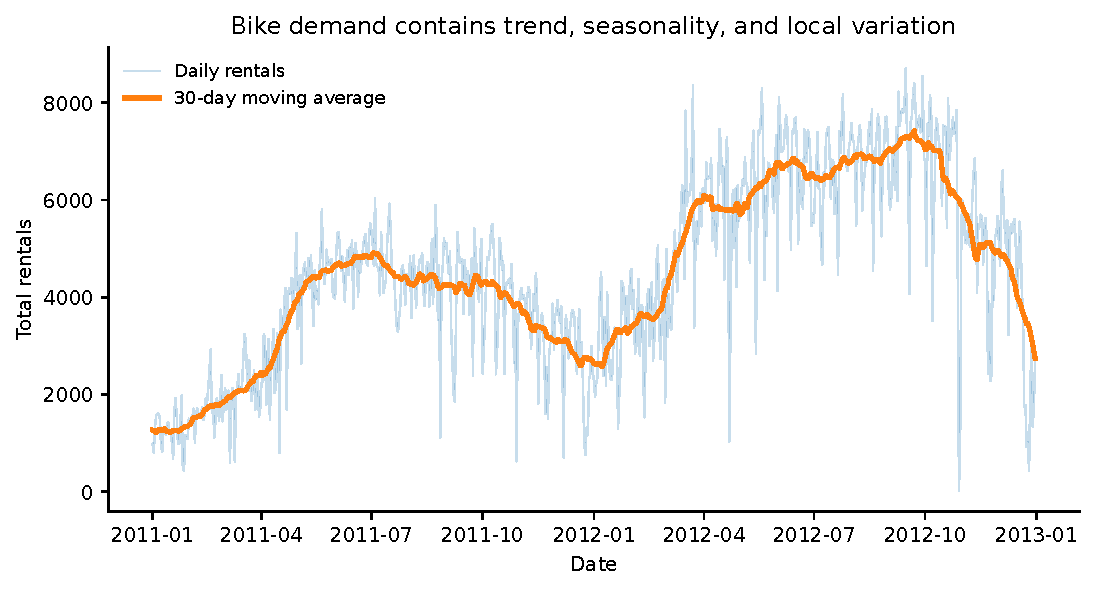
\includegraphics[width=0.88\linewidth]{figures/workflow_bike_daily_pattern.pdf}
\end{utpfig}

In this file, mean demand is about 4,504 rentals per day and normalized temperature has a correlation of about 0.63 with total demand. Neither number is a complete answer. Temperature changes with season, demand changes over calendar time, and working-day status changes the mix of casual and registered users. The workflow therefore moves from a first summary to progressively more careful questions rather than treating the first coefficient as the conclusion.

\begin{keyidea}
The first professional judgment is often not which model to fit, but which comparisons are legitimate given the unit of observation, time ordering, sampling process, and intended claim.
\end{keyidea}

\labsection{1}{Frame a question and build a reproducible data profile}{sec:lab01}

\begin{labproject}{Guided workflow: from question to evidence}
\textbf{Coverage.} Chapter~\ref{ch:workflow}.\\
\textbf{Goal.} By the end of the lab, you should be able to frame an estimable question, distinguish analytical roles of variables, construct a compact data profile, and document the computational environment that produced the result.\\
\textbf{Dataset.} \texttt{bike\_sharing\_dataset\_day.csv}.\\
\textbf{Scenario.} A bike-sharing operator wants a concise first assessment of daily demand. Before modelling anything, the analyst must define what one row means, identify the variables that can support the question, and produce an analysis another person can reproduce.

\textbf{Core workflow.}
\begin{enumerate}
  \item \textbf{Define the observational unit.} State precisely what one row represents. Classify \texttt{instant}, \texttt{dteday}, weather/context variables, \texttt{casual}, \texttt{registered}, and \texttt{cnt} as identifiers, context, predictors, component measures, or outcomes.
  \item \textbf{Audit before analysing.} Parse \texttt{dteday} as a date; report row/column counts, variable classes, missing values, and the date range. Confirm that \texttt{cnt = casual + registered} for every row.
  \item \textbf{Write three questions first.} Formulate one descriptive question, one comparative question, and one relational question. For each, name the quantity you will estimate before computing it.
  \item \textbf{Establish a baseline.} Summarise daily rental demand with center, spread, and range. Explain why a single mean is not an adequate description of a two-year time series.
  \item \textbf{Compare groups.} Contrast working and non-working days using both mean and median demand. Report group sizes so the comparison is interpretable.
  \item \textbf{Examine a relationship.} Quantify the association between normalised temperature and total rentals, then identify at least two variables that could partly explain that association.
  \item \textbf{Inspect time structure.} Plot demand over time and add a simple moving average. Identify trend, seasonal structure, abrupt changes, or periods that deserve further investigation.
  \item \textbf{Record reproducibility evidence.} Save the input path, analysis script, random seed if used, and \cmd{sessionInfo()} output. The result should be reproducible from a clean R session.
\end{enumerate}

\tcbbreak
\textbf{Executable experiment.} Run the file below from a clean R session, then modify it so your submitted questions and evidence are your own.
\lstinputlisting[style=utpr]{all_experiments/lab01_workflow.R}
\begin{verification}
\textbf{Required evidence.} Submit a one-page analysis note containing: the observational unit; the three questions; a compact data-profile summary; one time-series figure; two numerical findings; and one limitation. Every finding must be written as a complete evidence statement, not as raw console output.

\textbf{Decision checkpoint.} End with one recommendation for the \emph{next analysis step}. Examples include modelling seasonality, separating casual from registered users, or investigating weather effects. State what additional evidence would be needed before making an operational decision.
\end{verification}
\end{labproject}


\chapter{Data Types and Data Quality}
\label{ch:quality}
\chapterguide
  {You should be able to load a CSV and inspect its rows, columns, and summaries.}
  {classify variable roles; audit missingness, duplicates, validity, and consistency; and document defensible cleaning decisions.}

\section{Type means more than storage format}
R reports storage classes such as numeric or character, but analysis also depends on measurement meaning.

\begin{utptable}
\begin{tabularx}{\linewidth}{@{}>{\bfseries\leavevmode\color{UTPNavy}}m{2.7cm}D{4.1cm}Y@{}}
\toprule
\rowcolor{UTPPaleBlue!92}
\utpth{Analytical type} & \utpth{Example} & \utpth{Appropriate operations} \\
\midrule
Identifier & sample ID & matching, uniqueness checks; not averages \\
Nominal category & species, diagnosis & counts, proportions, group comparisons \\
Ordinal category & low / medium / high & ordered comparisons; spacing is not guaranteed equal \\
Numeric measurement & length, radius & summaries, differences, models \\
Target / outcome & malignant or benign & evaluation against predictions \\
\bottomrule
\end{tabularx}
\end{utptable}

\begin{pitfall}
A number is not automatically quantitative. Student ID 1042 plus Student ID 1043 does not create a meaningful sum. Analytical meaning determines what operations are valid.
\end{pitfall}


\section{Quality is fitness for a specific purpose}
There is no dataset that is simply ``clean'' in the abstract. Quality means that the data are sufficiently accurate, complete, consistent, timely, and appropriately sampled for a particular question. A missing measurement may be harmless for one summary and fatal for another model. A duplicated transaction may be legitimate if the unit of analysis is a transaction, but a serious error if the table is supposed to contain one row per customer.

\begin{utpfig}[Data quality is question-dependent]{The same table can be adequate for one task and inadequate for another because different questions depend on different fields and assumptions.}{fig:quality-purpose}
\begin{tikzpicture}[x=\linewidth,y=1cm,
  sourcecard/.style={draw=UTPBlue!75,fill=UTPPaleBlue,rounded corners=1.8mm,
    line width=0.75pt,text width=0.15\linewidth,
    minimum width=0.19\linewidth,minimum height=1.15cm,
    inner xsep=3mm,inner ysep=2.5mm,align=center,
    font=\scriptsize\color{UTPNavy}},
  taskcard/.style={draw=UTPBlue!65,fill=UTPPaleBlue,rounded corners=1.8mm,
    line width=0.7pt,text width=0.21\linewidth,
    minimum width=0.255\linewidth,minimum height=1.05cm,
    inner xsep=3.5mm,inner ysep=2mm,align=left,
    font=\scriptsize\color{UTPNavy}},
  qualityflow/.style={-{Stealth[length=2mm,width=1.5mm]},
    line width=0.85pt,draw=UTPTeal}]
\node[sourcecard] (data) at (0.12,0)
  {\textcolor{UTPBlue}{\textbf{SHARED INPUT}}\\[3pt]
   The same dataset};
\node[taskcard] (q1) at (0.43,0.80)
  {\textcolor{UTPBlue}{\textbf{QUESTION A}}\\[3pt]
   Requires a complete target.};
\node[taskcard] (q2) at (0.43,-0.80)
  {\textcolor{UTPBlue}{\textbf{QUESTION B}}\\[3pt]
   Requires reliable dates.};
\node[taskcard,draw=UTPTeal!80,fill=UTPPaleTeal] (a1) at (0.78,0.80)
  {\textcolor{UTPTeal}{\textbf{QUALITY CHECK}}\\[3pt]
   Is the target complete and reliable?};
\node[taskcard,draw=UTPTeal!80,fill=UTPPaleTeal] (a2) at (0.78,-0.80)
  {\textcolor{UTPTeal}{\textbf{QUALITY CHECK}}\\[3pt]
   Are the dates complete and valid?};
\coordinate (split) at (0.275,0);
\draw[draw=UTPTeal,line width=0.85pt] (data.east) -- (split);
\draw[qualityflow] (split) |- (q1.west);
\draw[qualityflow] (split) |- (q2.west);
\draw[qualityflow] (q1.east) -- (a1.west);
\draw[qualityflow] (q2.east) -- (a2.west);
\fill[UTPTeal] (split) circle (1.3pt);
\end{tikzpicture}
\end{utpfig}

\section{Four dimensions of a practical data audit}
\begin{utpfig}[Quality audit]{A quality audit asks whether the data are complete enough, internally valid, consistently represented, and uniquely recorded for the intended analysis.}{fig:quality-audit}
\begin{tikzpicture}[x=\linewidth,y=1cm,
  auditroot/.style={draw=UTPTeal!80,fill=UTPPaleTeal,rounded corners=5mm,
    line width=0.75pt,text width=0.17\linewidth,minimum height=0.90cm,
    inner xsep=3mm,inner ysep=2mm,align=center,
    font=\scriptsize\color{UTPNavy}},
  auditcard/.style={draw=UTPBlue!65,fill=UTPPaleBlue,rounded corners=1.8mm,
    line width=0.7pt,text width=0.235\linewidth,
    minimum width=0.29\linewidth,minimum height=1.15cm,
    inner xsep=4mm,inner ysep=2.5mm,align=left,
    font=\footnotesize\color{UTPNavy}},
  auditflow/.style={-{Stealth[length=2mm,width=1.5mm]},
    line width=0.8pt,draw=UTPTeal}]
\node[auditroot] (audit) at (0.50,0)
  {\textbf{QUALITY AUDIT}\\[3pt]
   \color{UTPMuted}fit for purpose};
\node[auditcard] (c) at (0.20,1.00)
  {\textcolor{UTPBlue}{\textbf{01  COMPLETENESS}}\\[4pt]
   Missing values};
\node[auditcard] (v) at (0.80,1.00)
  {\textcolor{UTPBlue}{\textbf{02  VALIDITY}}\\[4pt]
   Plausible ranges};
\node[auditcard] (s) at (0.20,-1.00)
  {\textcolor{UTPBlue}{\textbf{03  CONSISTENCY}}\\[4pt]
   Labels and units};
\node[auditcard] (u) at (0.80,-1.00)
  {\textcolor{UTPBlue}{\textbf{04  UNIQUENESS}}\\[4pt]
   Duplicate records};
\draw[auditflow] (audit.west) to[out=160,in=0] (c.east);
\draw[auditflow] (audit.east) to[out=20,in=180] (v.west);
\draw[auditflow] (audit.west) to[out=200,in=0] (s.east);
\draw[auditflow] (audit.east) to[out=-20,in=180] (u.west);
\end{tikzpicture}
\end{utpfig}


\begin{utpfig}[A row-level quality map]{The deliberately corrupted Iris dataset contains missing and invalid values. A map makes concentration and co-occurrence visible, which a single missing-value count cannot show.}{fig:quality-map}
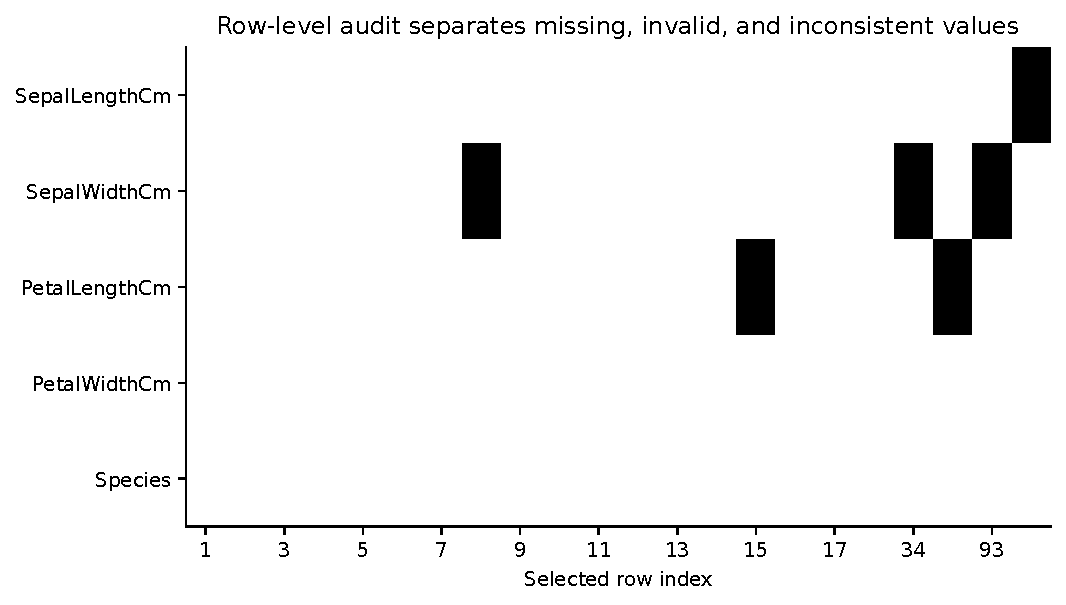
\includegraphics[width=0.93\linewidth]{figures/quality_missingness_map.pdf}
\end{utpfig}


Missingness is not just a count. Ask \emph{which variable is missing, for which records, and whether the absence itself could be informative}. A cleaning rule that is harmless for one question can bias another.

\section{Validity rules come from the domain}
A positive physical length cannot be negative. A probability must lie between 0 and 1. A date of discharge should not precede admission. These are semantic constraints, not software constraints.

\begin{lstlisting}[style=utpr]
invalid <- iris$SepalLengthCm <= 0 |
           iris$SepalWidthCm <= 0
sum(invalid, na.rm = TRUE)
\end{lstlisting}


\section{Missing-data mechanisms change what is defensible}
The cause of missingness matters. Three common conceptual cases are useful:
\begin{itemize}
  \item \textbf{Missing completely at random (MCAR):} absence is unrelated to measured or unmeasured values. Complete-case analysis may remain unbiased, although less precise.
  \item \textbf{Missing at random (MAR):} absence can be explained by observed variables. Conditional imputation or modelling may be defensible if those predictors are included.
  \item \textbf{Missing not at random (MNAR):} absence depends on the missing value itself or another unobserved factor. Sensitivity analysis and domain knowledge become important because the missingness process cannot be repaired mechanically from observed columns alone.
\end{itemize}
These labels are assumptions about the data-generating process, not properties that software can determine with certainty from the table.


\section{Missing data: deletion, imputation, or model explicitly}
There is no universally correct treatment.
\begin{itemize}
  \item \textbf{Delete} when missingness is small and plausibly unrelated to the outcome, and report how many rows were removed.
  \item \textbf{Impute} when preserving rows is important and a defensible replacement rule exists.
  \item \textbf{Model missingness} or add an indicator when the absence itself may carry information.
\end{itemize}

Simple median imputation is robust to extreme values but reduces apparent variability. It is suitable as a teaching method, not a reason to ignore why values are missing.


\begin{utpfig}[Cleaning changes the evidence]{Applying a validity rule can visibly change a distribution. The analyst should compare before and after, count affected rows, and document why the rule is justified.}{fig:quality-cleaning-change}
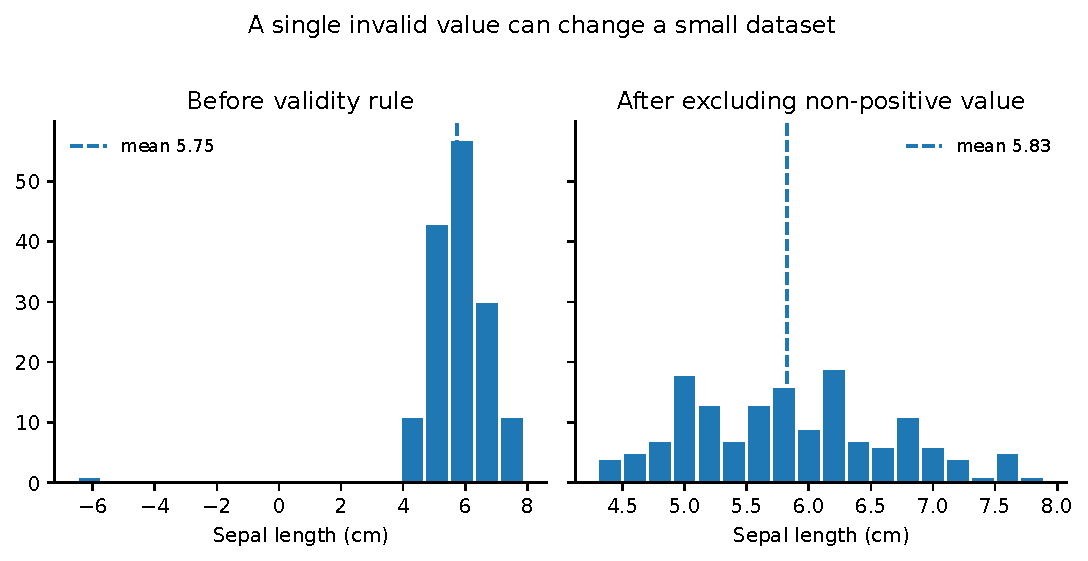
\includegraphics[width=0.82\linewidth]{figures/quality_cleaning_distribution.pdf}
\end{utpfig}

\section{Keys, duplicates, and unit-of-observation errors}
A duplicate is defined relative to an expected key. Exact duplicated rows are easy to find, but more important problems include duplicated identifiers with conflicting values and repeated observations that are legitimate but accidentally treated as independent entities. Before removing anything, determine the intended key and whether repeated keys are expected.

\begin{lstlisting}[style=utpr]
# Are IDs unique when they should be?
anyDuplicated(iris$Id)

# Which IDs repeat?
iris$Id[duplicated(iris$Id)]
\end{lstlisting}

\section{Duplicates and inconsistent categories}
Exact duplicates can inflate counts and train/test performance. Inconsistent labels such as \cmd{"Iris-setosa"}, \cmd{"iris setosa"}, and \cmd{"SETOSA"} represent one concept but appear as three categories until standardised.

\begin{workedexample}
A defensible cleaning log records the rule and the evidence:
\begin{utptable}
\begin{tabularx}{\linewidth}{@{}>{\bfseries\leavevmode\color{UTPNavy}}m{3.2cm}D{4.5cm}Y@{}}
\toprule
\rowcolor{UTPPaleBlue!92}
\utpth{Issue} & \utpth{Rule} & \utpth{Evidence retained} \\
\midrule
Duplicate row & keep first exact record & duplicate count before/after \\
Negative length & mark impossible value missing & row identifier and rule \\
Missing measurement & median within species & imputation method and affected count \\
Label variant & normalise case/spacing & original and standard labels \\
\bottomrule
\end{tabularx}
\end{utptable}
\end{workedexample}


\section{Measurement error and label quality}
Not every bad value is impossible. Measurements can be noisy even when they lie in a plausible range, and labels can be incorrect even when they use a valid category name. This distinction matters because a range check finds impossible values but not subtle measurement error.

For supervised learning, target quality is especially important. If diagnosis labels contain errors, the model is trained to reproduce those errors. Apparent model ``mistakes'' may sometimes reveal ambiguous or mislabeled examples rather than algorithm failure.


\section{Leakage: a quality problem for modelling}
\term{Data leakage} occurs when information unavailable at prediction time enters model training. Examples include using a final diagnosis to construct an input feature or scaling the entire dataset before the train/test split. Leakage produces optimistic evaluation, even when the code runs correctly.

\begin{keyidea}
Cleaning is an analytical decision. A good report states what changed, why it changed, how many records were affected, and what uncertainty the change creates.
\end{keyidea}


\begin{utpfig}[Leakage is information arriving from the future]{A modelling feature is legitimate only if it would be available at the moment a real prediction must be made. Post-outcome information can make validation look excellent while making deployment impossible.}{fig:leakage-timeline}
\begin{tikzpicture}[x=1cm,y=1cm]
\draw[-{Stealth[length=2.5mm]},thick,draw=UTPMuted] (-5,0)--(5,0);
\node[tagb] at (-4.1,0.6) {information available};
\node[tagb] at (0,0.65) {prediction time};
\node[tagb] at (4.0,0.6) {outcome known};
\draw[thick,UTPTeal] (0,-0.28)--(0,0.28);
\node[fcbox,text width=3.0cm] at (-2.8,-1.0) {valid features\\measurements before decision};
\node[cellbad,minimum width=4.0cm,minimum height=1.15cm,align=center] at (2.8,-1.0) {leaky features\\treatment or information created after outcome};
\end{tikzpicture}
\end{utpfig}

\begin{quickcheck}
\begin{enumerate}
  \item Why should identifiers usually be excluded from averages and predictive features?
  \item What makes a range check different from a missing-value check?
  \item Why can median imputation make a distribution look less variable than it really is?
  \item Give one example of data leakage.
\end{enumerate}
\end{quickcheck}

\section{Worked audit: two datasets, two different quality stories}

Quality problems should be described in the language of the data rather than reduced to a single ``percent missing'' number. The bundled Iris file and Titanic file illustrate two distinct situations.

\begin{utpfig}[Iris quality audit]{The Iris file is small enough to inspect manually. It contains a few missing measurements and one inconsistent species label, showing that category consistency and completeness are separate dimensions of quality.}{fig:quality-iris-audit}
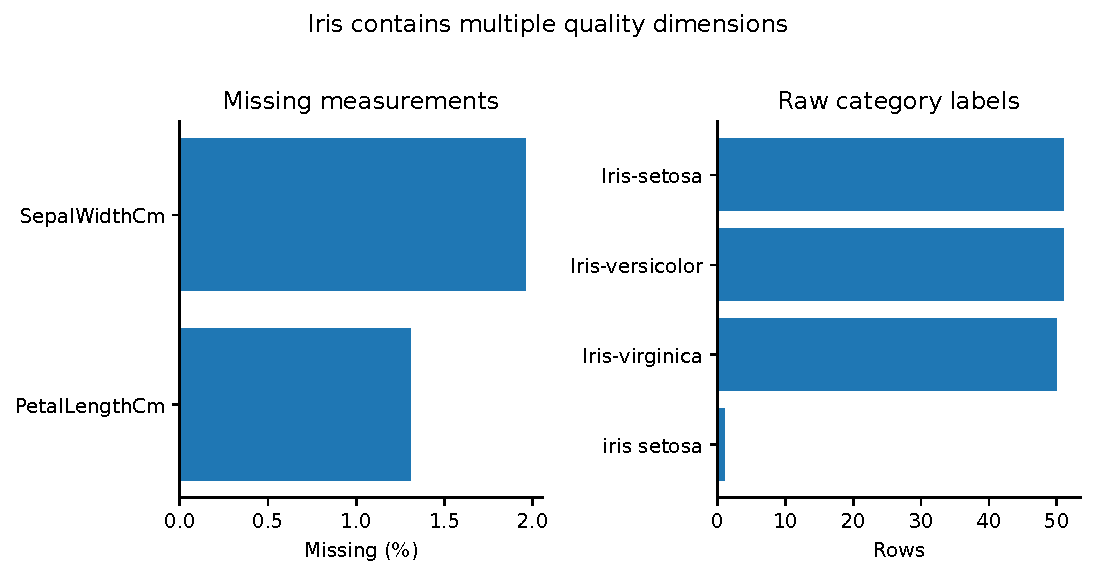
\includegraphics[width=0.88\linewidth]{figures/quality_iris_audit.pdf}
\end{utpfig}

The 153-row Iris file contains three missing \texttt{SepalWidthCm} values, two missing \texttt{PetalLengthCm} values, and a lower-case/space variant of the setosa label. Converting labels to a canonical form is usually low-risk because the intended semantic equivalence is clear. Imputing a flower measurement is a stronger analytical decision because it invents a value and can change correlations, group means, or downstream classification.

\begin{utpfig}[Titanic missingness is concentrated, not uniform]{About 77\% of \texttt{Cabin} and 20\% of \texttt{Age} are missing, whereas most variables are complete. This pattern calls for variable-specific reasoning rather than a blanket ``drop missing rows'' rule.}{fig:quality-titanic-missing}
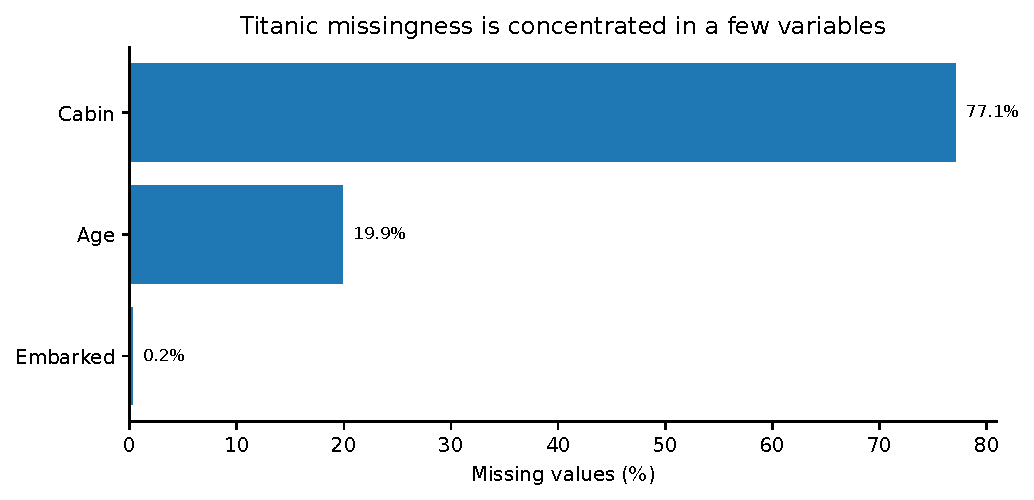
\includegraphics[width=0.82\linewidth]{figures/quality_titanic_missingness.pdf}
\end{utpfig}

Deleting every row with any missing value would discard most passengers because \texttt{Cabin} is frequently absent. A professional audit asks what ``missing'' means: was a cabin never recorded, not applicable, unreadable in the source, or simply lost during data assembly? The answer determines whether missingness is nuisance, information, or both.

\begin{workedexample}
A sensible teaching strategy for \texttt{Age} is to preserve the original column and create \cmd{Age\_imputed}. Group-median imputation by passenger class and sex is transparent and reproducible, but it still shrinks within-group variation. The report should therefore state how many values were imputed and avoid presenting the derived ages as observed facts.
\end{workedexample}


\section{Extended audit: structural missingness and duplicate semantics}

The Ames Housing and Red Wine Quality datasets show why a professional data-quality review must go beyond a generic missing-value function. In Ames, some variables are almost entirely missing, but the reason is often structural: a property without a pool has no meaningful pool-quality rating, and a property without an alley cannot have an alley type. Encoding those cases as ordinary numeric or categorical missingness without understanding the data dictionary can erase information.

\begin{utpfig}[Ames missingness has semantic structure]{The most incomplete fields are largely optional property attributes. A high missing percentage is therefore a prompt to investigate meaning, not an automatic instruction to drop the column.}{fig:quality-ames-missing}
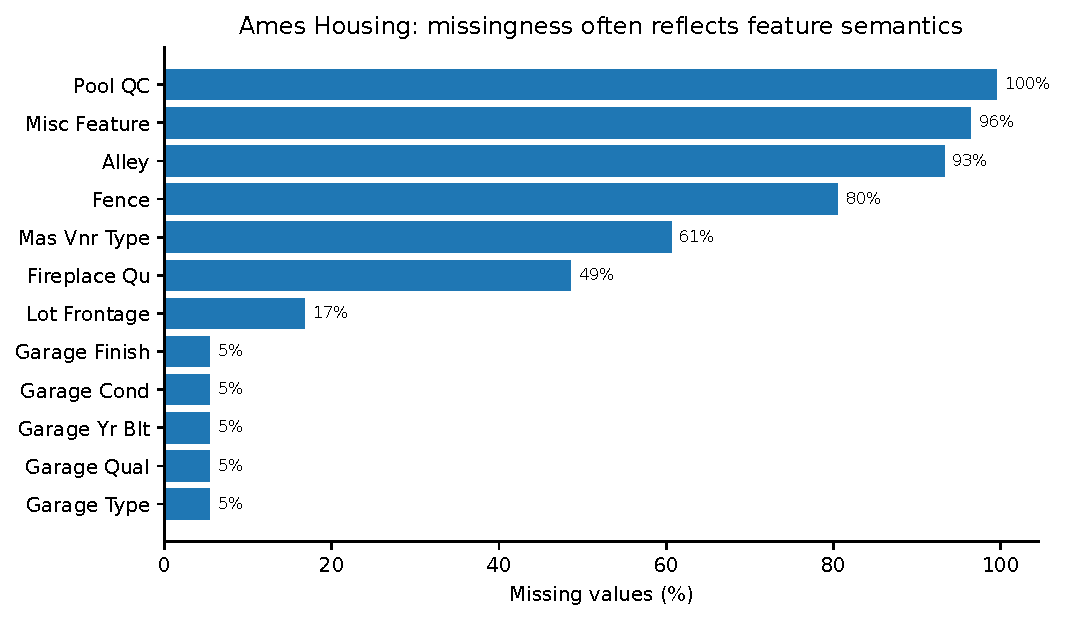
\includegraphics[width=0.86\linewidth]{figures/quality_ames_missingness.pdf}
\end{utpfig}

This distinction is useful in modelling. For a feature such as \texttt{Pool QC}, an explicit category such as ``No pool'' can carry different information from ``pool quality was not recorded.'' The analyst should preserve that distinction whenever the source permits it.

The Red Wine Quality file illustrates a different issue. It contains exact duplicate rows even though no unique wine identifier is supplied.

\begin{utpfig}[Duplicate rows require a definition of the observational unit]{The file has fewer unique rows than supplied rows. That fact alone does not establish an error: two wines can share the same measured chemistry and quality score, or the same record may have been repeated.}{fig:quality-wine-duplicates}
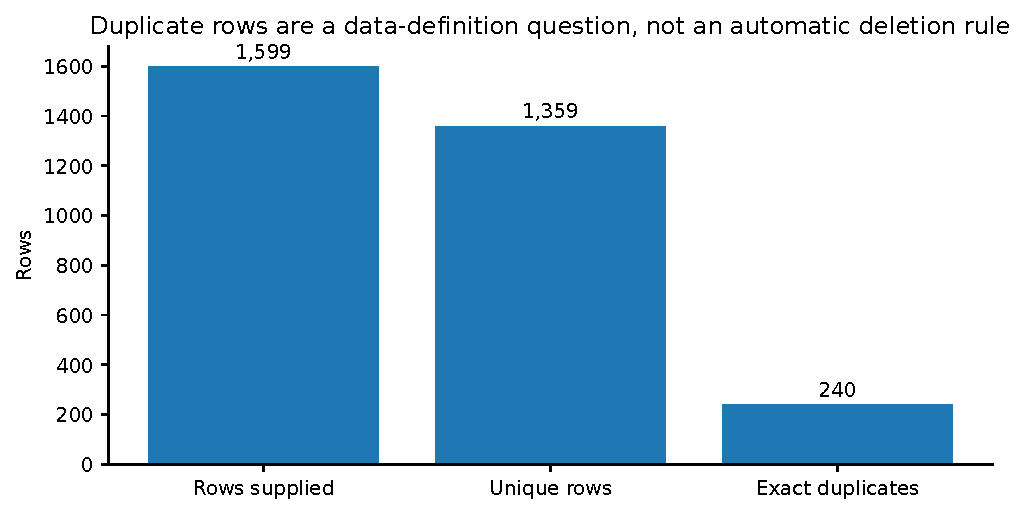
\includegraphics[width=0.72\linewidth]{figures/quality_wine_duplicates.pdf}
\end{utpfig}

\begin{keyidea}
Never write \cmd{distinct()} or \cmd{duplicated()} as a cleaning ritual. First state the expected key and the intended unit of observation, then explain why repeated rows are impossible, possible, or informative under that definition.
\end{keyidea}

\labsection{2}{Audit missingness, categories, and validity}{sec:lab02}

\begin{labproject}{Data-quality audit: define rules before cleaning}
\textbf{Coverage.} Chapter~\ref{ch:quality}.\\
\textbf{Goal.} You should be able to distinguish missingness, invalid values, inconsistent categories, duplicate records, and structural absence; then choose a defensible treatment based on variable meaning and analytical purpose.\\
\textbf{Datasets.} \texttt{iris\_dataset.csv} and \texttt{titanic\_dataset.csv}; Ames Housing and Red Wine Quality are used as extensions.\\
\textbf{Scenario.} You have received data from multiple sources and must decide whether it is fit for analysis. The objective is not to make the data ``look clean'', but to identify defects, document rules, and preserve an auditable record of every transformation.

\textbf{Core audit.}
\begin{enumerate}
  \item \textbf{Create a quality profile.} For both primary datasets, report dimensions, variable classes, key uniqueness, and missing count/percentage for every variable.
  \item \textbf{Define validity rules.} Write rules before testing them: positive flower measurements; valid Titanic class and survival codes; non-negative fares; and plausible identifier uniqueness.
  \item \textbf{Standardise categories safely.} Inspect raw Iris species labels, create a new cleaned label, and verify that accidental spelling/format variants collapse to the intended categories. Do not overwrite the raw field.
  \item \textbf{Investigate missingness.} For Titanic, compare the concentration of missing values across \texttt{Age}, \texttt{Cabin}, and \texttt{Embarked}. Explain why one treatment is not appropriate for all three variables.
  \item \textbf{Demonstrate transparent imputation.} Create \texttt{Age\_imputed} using a documented group-median rule while preserving \texttt{Age}. Report how many values were changed and which grouping variables determined the replacement.
  \item \textbf{Check consequences.} Compare the age distribution before and after imputation. State one benefit and one distortion that the chosen rule can introduce.
\end{enumerate}

\begin{tryit}
\textbf{Extension A---structural missingness.} In \texttt{ames\_housing\_dataset.csv}, inspect variables with the highest missingness. Identify at least three fields where missing may mean ``feature absent'' rather than ``measurement unknown''. Explain how that semantic distinction changes preprocessing.

\textbf{Extension B---duplicate semantics.} In \texttt{red\_wine\_quality\_dataset.csv}, count exact duplicate rows. Before removing any, define the intended observational unit and explain why identical measurements do not automatically prove that a row is erroneous.
\end{tryit}

\tcbbreak
\lstinputlisting[style=utpr]{all_experiments/lab02_data_quality.R}
\begin{verification}
\textbf{Required evidence.} Submit a data-quality log with each issue written as \emph{rule $\rightarrow$ evidence $\rightarrow$ action $\rightarrow$ consequence}. Include at least one issue you deliberately leave unchanged because the evidence is insufficient to justify a transformation.

\textbf{Professional standard.} A cleaning step is acceptable only when another analyst can determine what changed, why it changed, and whether the original value is still recoverable.
\end{verification}
\end{labproject}



\part{Working with Data and Finding Patterns}
\chapter{Data Wrangling and Feature Construction}
\label{ch:wrangling}
\chapterguide
  {You should understand observations, variables, data types, and data-quality checks.}
  {select and filter records, sort data, compute grouped summaries, and create features that preserve clear meaning.}

\section{Wrangling changes representation, not the question}
Data wrangling prepares the evidence needed for analysis. Common operations are selecting variables, filtering observations, ordering records, grouping categories, aggregating summaries, joining tables, and constructing derived features.

\begin{utpfig}[Wrangling pipeline]{Each operation should be explainable as a transformation from one table to another.}{fig:wrangling-pipeline}
\begin{tikzpicture}[x=\linewidth,y=1cm,
  stage/.style={draw=UTPBlue!65,fill=UTPPaleBlue,rounded corners=1.8mm,
    line width=0.7pt,text width=0.14\linewidth,
    minimum width=0.18\linewidth,minimum height=1.70cm,
    inner xsep=2.5mm,inner ysep=2.5mm,align=center,
    font=\scriptsize\color{UTPNavy}},
  endpoint/.style={stage,draw=UTPTeal!80,fill=UTPPaleTeal},
  flow/.style={-{Stealth[length=2mm,width=1.5mm]},
    line width=0.9pt,draw=UTPTeal}]
\node[endpoint] (raw) at (0.10,0)
  {\textcolor{UTPTeal}{\textbf{01  INPUT}}\\[5pt]
   \textbf{Raw table}\\[3pt]
   Original records\\and variables};
\node[stage] (sel) at (0.30,0)
  {\textcolor{UTPBlue}{\textbf{02  SCOPE}}\\[5pt]
   \textbf{Select and filter}\\[3pt]
   Relevant rows\\and columns};
\node[stage] (feat) at (0.50,0)
  {\textcolor{UTPBlue}{\textbf{03  DERIVE}}\\[5pt]
   \textbf{Create features}\\[3pt]
   Interpretable\\derived variables};
\node[stage] (grp) at (0.70,0)
  {\textcolor{UTPBlue}{\textbf{04  SUMMARISE}}\\[5pt]
   \textbf{Aggregate}\\[3pt]
   Summaries at\\the required grain};
\node[endpoint] (ana) at (0.90,0)
  {\textcolor{UTPTeal}{\textbf{05  OUTPUT}}\\[5pt]
   \textbf{Analysis table}\\[3pt]
   Evidence for\\the question};
\draw[flow] (raw.east) -- (sel.west);
\draw[flow] (sel.east) -- (feat.west);
\draw[flow] (feat.east) -- (grp.west);
\draw[flow] (grp.east) -- (ana.west);
\end{tikzpicture}
\end{utpfig}


\section{Think in verbs: each step should have one purpose}
A readable wrangling pipeline is a sequence of simple verbs: \emph{select}, \emph{filter}, \emph{mutate}, \emph{group}, \emph{summarise}, \emph{join}, and \emph{reshape}. Keeping transformations small makes intermediate row counts and assumptions easier to audit.

\begin{utpfig}[Table transformations as contracts]{Each transformation should preserve a clear contract: what one row represents, which variables are retained, and which new values were derived.}{fig:wrangle-contract}
\begin{tikzpicture}[node distance=0.14cm,
  stage/.style={draw=UTPBlue!65,fill=UTPPaleBlue,rounded corners=1.8mm,
    line width=0.7pt,text width=0.70\linewidth,
    minimum width=0.76\linewidth,minimum height=0.84cm,
    inner xsep=5mm,inner ysep=1.3mm,align=left,
    font=\scriptsize\color{UTPNavy}},
  endpoint/.style={stage,draw=UTPTeal!80,fill=UTPPaleTeal},
  flow/.style={-{Stealth[length=1.8mm,width=1.4mm]},
    line width=0.9pt,draw=UTPTeal},
  stagejoin/.style={line width=0.75pt,draw=UTPTeal}]
\node[endpoint] (a)
  {\textcolor{UTPTeal}{\textbf{01  INPUT CONTRACT}}\\[3pt]
   One row = one wine sample; 15 variables};
\node[stage,below=of a] (b)
  {\textcolor{UTPBlue}{\textbf{02  SELECT}}\\[3pt]
   Keep cultivar, alcohol, colour intensity, and proline};
\node[stage,below=of b] (c)
  {\textcolor{UTPBlue}{\textbf{03  FILTER}}\\[3pt]
   Retain records meeting a stated inclusion rule};
\node[stage,below=of c] (d)
  {\textcolor{UTPBlue}{\textbf{04  CREATE FEATURES}}\\[3pt]
   Add interpretable derived columns};
\node[endpoint,below=of d] (e)
  {\textcolor{UTPTeal}{\textbf{05  OUTPUT CONTRACT}}\\[3pt]
   One row still = one wine sample; analysis-ready variables};
\coordinate (r1) at ([xshift=-7mm]a.west);
\coordinate (r2) at ([xshift=-7mm]b.west);
\coordinate (r3) at ([xshift=-7mm]c.west);
\coordinate (r4) at ([xshift=-7mm]d.west);
\coordinate (r5) at ([xshift=-7mm]e.west);
\draw[flow] ([yshift=3mm]r1) -- ([yshift=-3mm]r5);
\foreach \rail/\card in {r1/a,r2/b,r3/c,r4/d,r5/e}{
  \draw[stagejoin] (\rail) -- (\card.west);
  \fill[UTPTeal] (\rail) circle (1.15pt);
}
\end{tikzpicture}
\end{utpfig}

\section{Select only what the question needs}
If the question concerns alcohol, colour intensity, and cultivar, carrying every available variable into every step increases cognitive load and opportunities for mistakes.

\begin{lstlisting}[style=utpr]
analysis <- wine[, c("cultivar", "alcohol",
                     "color_intensity", "proline")]
\end{lstlisting}

\section{Filter records with explicit conditions}
Filtering defines the population being analysed. That means every filter should be stated in the report.

\begin{lstlisting}[style=utpr]
high_alcohol <- wine[wine$alcohol >= 13.5, ]
\end{lstlisting}

\begin{pitfall}
Filtering after looking at the outcome can quietly turn exploration into cherry-picking. Define inclusion rules from the analytical question or domain constraints, and disclose post-hoc filters.
\end{pitfall}


\section{Aggregation changes the unit of observation}
When rows are grouped and summarised, the output table no longer represents individual observations. One row may now represent a cultivar, region, month, or customer. This is a fundamental change in the analytical unit and should be made explicit.

\begin{utpfig}[Grouped means with uncertainty]{The cultivar means differ, while the dashed line shows the overall mean. Error bars are approximate 95\% intervals for each group mean and remind us that summaries are estimates.}{fig:wrangle-group-summary}
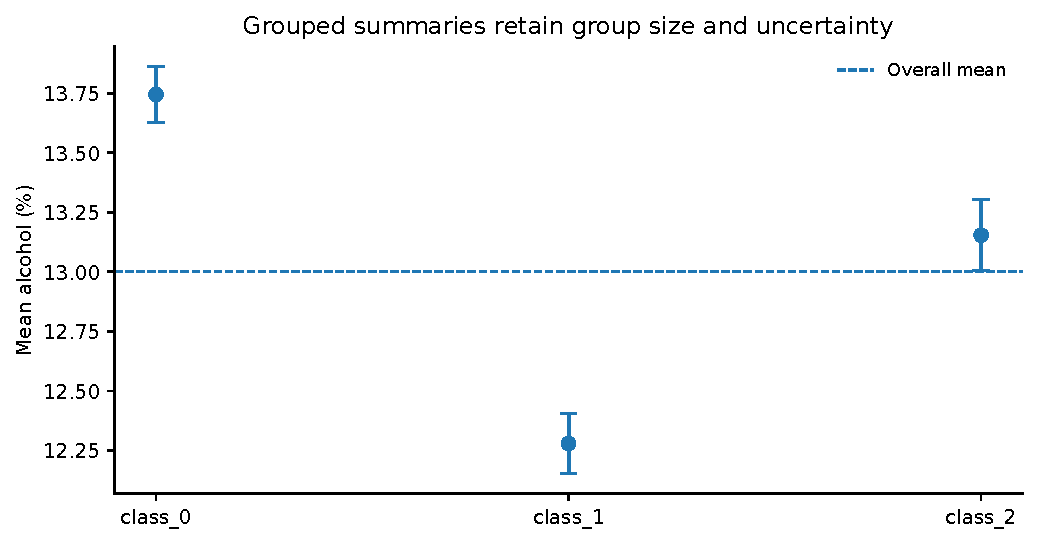
\includegraphics[width=0.80\linewidth]{figures/wrangling_group_summary.pdf}
\end{utpfig}


\begin{utpfig}[A transformation changes scale and shape]{The log transformation compresses large values more strongly than small values. It can make skewed data easier to visualise or model, but it also changes coefficient interpretation.}{fig:wrangle-transform}
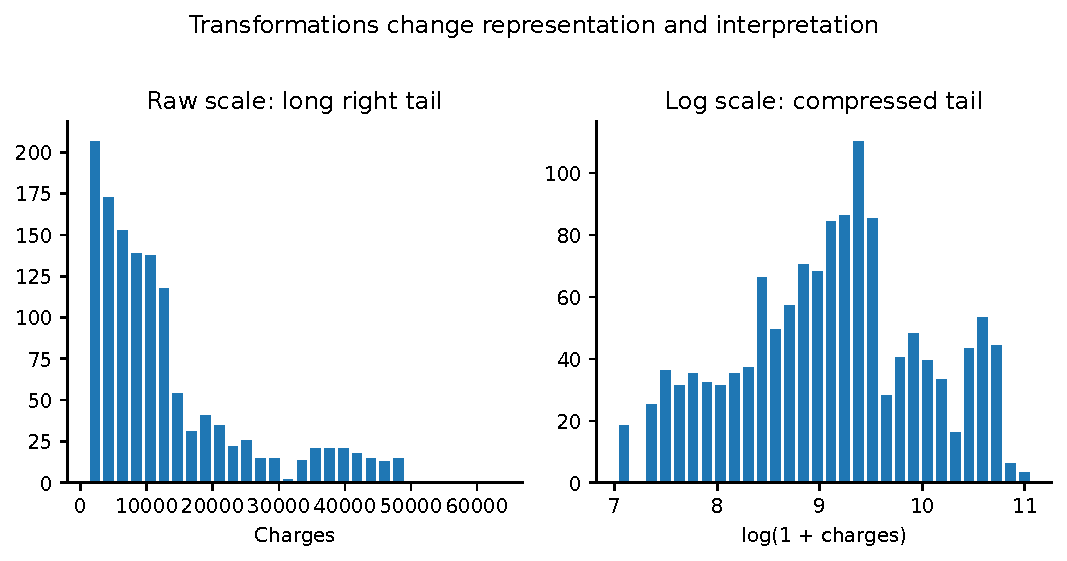
\includegraphics[width=0.82\linewidth]{figures/wrangling_transform.pdf}
\end{utpfig}

\begin{keyidea}
Always ask whether a grouped result is weighted correctly for the question. Averaging three group means is not generally the same as the overall mean when group sizes differ.
\end{keyidea}

\section{Grouped summaries reveal structured differences}
Overall averages can hide subgroup structure. The \cmd{aggregate()} function makes the comparison explicit:
\begin{lstlisting}[style=utpr]
aggregate(alcohol ~ cultivar, data = wine, FUN = mean)
\end{lstlisting}
A group summary should usually include both a center and a measure of spread or sample size.


\section{Reshaping: wide and long representations}
The same information can be represented in different table shapes. \term{Wide} data often place repeated measures in separate columns, while \term{long} data place the measurement name and value in rows. Long form is often convenient for grouped plotting and repeated-measures analysis; wide form can be convenient for modelling matrices.

\begin{utpfig}[Wide and long are representations of the same information]{Reshaping should change layout, not invent or discard measurements. The key columns must be sufficient to reconstruct the original representation.}{fig:wide-long}
\begin{tikzpicture}[x=\linewidth,y=1cm,
  tablecard/.style={draw=UTPBlue!65,fill=UTPPaleBlue,rounded corners=1.8mm,
    line width=0.7pt,text width=0.36\linewidth,
    minimum width=0.42\linewidth,minimum height=4.05cm,
    inner sep=3mm,align=center,font=\scriptsize\color{UTPNavy}},
  reshapebadge/.style={draw=UTPTeal!80,fill=UTPPaleTeal,
    rounded corners=4mm,line width=0.75pt,text width=0.075\linewidth,
    minimum height=0.78cm,inner xsep=2mm,inner ysep=1.5mm,
    align=center,font=\scriptsize\bfseries\color{UTPTeal}},
  reshape/.style={-{Stealth[length=2mm,width=1.5mm]},
    line width=0.85pt,draw=UTPTeal}]
\node[tablecard] (wide) at (0.22,0) {%
  \begin{minipage}[t][3.35cm][t]{\linewidth}
  \setlength{\parskip}{0pt}
  \centering
  \textcolor{UTPBlue}{\textbf{01  WIDE FORMAT}}\\[3pt]
  \textbf{One row per ID}\\[1pt]
  Repeated measures occupy columns\par\vspace{4pt}
  \fontsize{7.4}{8.8}\selectfont
  \renewcommand{\arraystretch}{1.02}
  \setlength{\tabcolsep}{5pt}
  \setlength{\extrarowheight}{0pt}
  \arrayrulecolor{UTPBlue!45}
  \begin{tabular}{@{}crr@{}}
  \rowcolor{UTPBlue!85}
  \textcolor{white}{\textbf{ID}} &
  \textcolor{white}{\textbf{Morning}} &
  \textcolor{white}{\textbf{Evening}} \\
  \rowcolor{white}
  01 & 21.4 & 26.1 \\
  \rowcolor{UTPBlue!5}
  02 & 20.9 & 25.6 \\
  \bottomrule
  \end{tabular}
  \end{minipage}};
\node[tablecard,draw=UTPTeal!80,fill=UTPPaleTeal] (long) at (0.78,0) {%
  \begin{minipage}[t][3.35cm][t]{\linewidth}
  \setlength{\parskip}{0pt}
  \centering
  \textcolor{UTPTeal}{\textbf{02  LONG FORMAT}}\\[3pt]
  \textbf{One row per ID and time}\\[1pt]
  Repeated measures occupy rows\par\vspace{4pt}
  \fontsize{7.4}{8.8}\selectfont
  \renewcommand{\arraystretch}{1.02}
  \setlength{\tabcolsep}{5pt}
  \setlength{\extrarowheight}{0pt}
  \arrayrulecolor{UTPTeal!45}
  \begin{tabular}{@{}clr@{}}
  \rowcolor{UTPTeal!85}
  \textcolor{white}{\textbf{ID}} &
  \textcolor{white}{\textbf{Time}} &
  \textcolor{white}{\textbf{Value}} \\
  \rowcolor{white}
  01 & morning & 21.4 \\
  \rowcolor{UTPTeal!5}
  01 & evening & 26.1 \\
  \rowcolor{white}
  02 & morning & 20.9 \\
  \rowcolor{UTPTeal!5}
  02 & evening & 25.6 \\
  \bottomrule
  \end{tabular}
  \end{minipage}};
\node[reshapebadge] (change) at (0.50,0)
  {RESHAPE};
\draw[reshape] (wide.east) -- (change.west);
\draw[reshape] (change.east) -- (long.west);
\node[font=\scriptsize\color{UTPMuted},align=center] at (0.50,-2.30)
  {same measurements \textbullet\ different layout};
\end{tikzpicture}
\end{utpfig}

\section{Feature engineering should add meaning}
A \term{feature} is an input variable used in analysis or modelling. New features can simplify relationships, encode domain knowledge, or make scales easier to compare.

\begin{utptable}
\begin{tabularx}{\linewidth}{@{}>{\bfseries\leavevmode\color{UTPNavy}}m{3.1cm}D{4.4cm}Y@{}}
\toprule
\rowcolor{UTPPaleBlue!92}
\utpth{Feature operation} & \utpth{Example} & \utpth{Reason} \\
\midrule
Binning & alcohol to lower/middle/higher & communicate broad ranges \\
Transformation & \(\log(1+x)\) & compress strongly right-skewed values \\
Ratio & cost per unit & represent relative rather than absolute size \\
Interaction & age \(\times\) treatment & allow one effect to vary with another \\
Indicator & missing = yes/no & preserve missingness as information \\
\bottomrule
\end{tabularx}
\end{utptable}

\begin{keyidea}
A good engineered feature has a sentence-level interpretation. If you cannot explain what the feature means without referring to the code that produced it, it is hard to defend analytically.
\end{keyidea}


\section{Join cardinality should be known before the join}
A join combines rows according to key matches. The expected relationship between keys is called \term{cardinality}. One-to-one joins should preserve row count; one-to-many joins deliberately repeat the ``one'' side; many-to-many joins can create a Cartesian multiplication and are frequently accidental.

\begin{utpfig}[Join cardinality]{Knowing the expected key relationship lets row-count changes become a diagnostic rather than a surprise.}{fig:join-cardinality}
\begin{tikzpicture}[x=\linewidth,y=1cm,
  relationship/.style={draw=UTPBlue!65,fill=UTPPaleBlue,
    rounded corners=1.8mm,line width=0.7pt,text width=0.235\linewidth,
    minimum width=0.29\linewidth,minimum height=2.70cm,
    inner xsep=4mm,inner ysep=3mm,
    align=center,font=\scriptsize\color{UTPNavy}}]
\node[relationship] (oneone) at (0.17,0)
  {\textcolor{UTPBlue}{\textbf{01  ONE-TO-ONE}}\\[5pt]
   {\fontsize{13}{15}\selectfont\bfseries 1 : 1}\\[6pt]
   One profile per ID\\One outcome per ID\\[6pt]
   \textcolor{UTPMuted}{\textbf{ROW COUNT}}\\[-1pt]
   Usually preserved};
\node[relationship,draw=UTPTeal!80,fill=UTPPaleTeal] (onemany) at (0.50,0)
  {\textcolor{UTPTeal}{\textbf{02  ONE-TO-MANY}}\\[5pt]
   {\fontsize{13}{15}\selectfont\bfseries 1 : many}\\[6pt]
   One customer\\Many transactions\\[6pt]
   \textcolor{UTPMuted}{\textbf{ROW COUNT}}\\[-1pt]
   Expected expansion};
\node[relationship,draw=UTPRed!80,fill=UTPPaleRed] (manymany) at (0.83,0)
  {\textcolor{UTPRed!85!black}{\textbf{03  MANY-TO-MANY}}\\[5pt]
   {\fontsize{13}{15}\selectfont\bfseries many : many}\\[6pt]
   Repeated keys\\on both sides\\[6pt]
   \textcolor{UTPRed!85!black}{\textbf{ROW COUNT}}\\[-1pt]
   Can multiply unexpectedly};
\end{tikzpicture}
\end{utpfig}

\section{Joining tables introduces a new failure mode}
When combining tables, the join key should be unique at the expected level. A many-to-many join can multiply rows and corrupt counts.

\begin{workedexample}
Before joining customer and transaction tables, verify whether customer ID is unique in the customer table and repeated in the transaction table. That expected one-to-many relationship is part of the data model, not an implementation detail.
\end{workedexample}

\begin{quickcheck}
\begin{enumerate}
  \item Why can an overall mean be misleading when groups differ strongly?
  \item What should be stated whenever rows are filtered out?
  \item Give one reason to log-transform a feature.
  \item What join problem can cause row counts to increase unexpectedly?
\end{enumerate}
\end{quickcheck}

\section{Worked case: from 17,379 hourly rows to an interpretable demand profile}

The hourly Bike Sharing file demonstrates why wrangling is analytical work rather than clerical preparation. One row represents one observed hour. The goal is not to make the table smaller for its own sake, but to create a representation matched to a question such as ``How does the daily demand pattern differ between working and non-working days?''

\begin{utpfig}[Aggregation exposes a behavioural pattern]{A grouped hourly summary reveals commuting peaks on working days and a broader daytime pattern on non-working days. The transformation changes the grain from individual observed hours to mean demand for each hour--day-type combination.}{fig:wrangle-bike-hours}
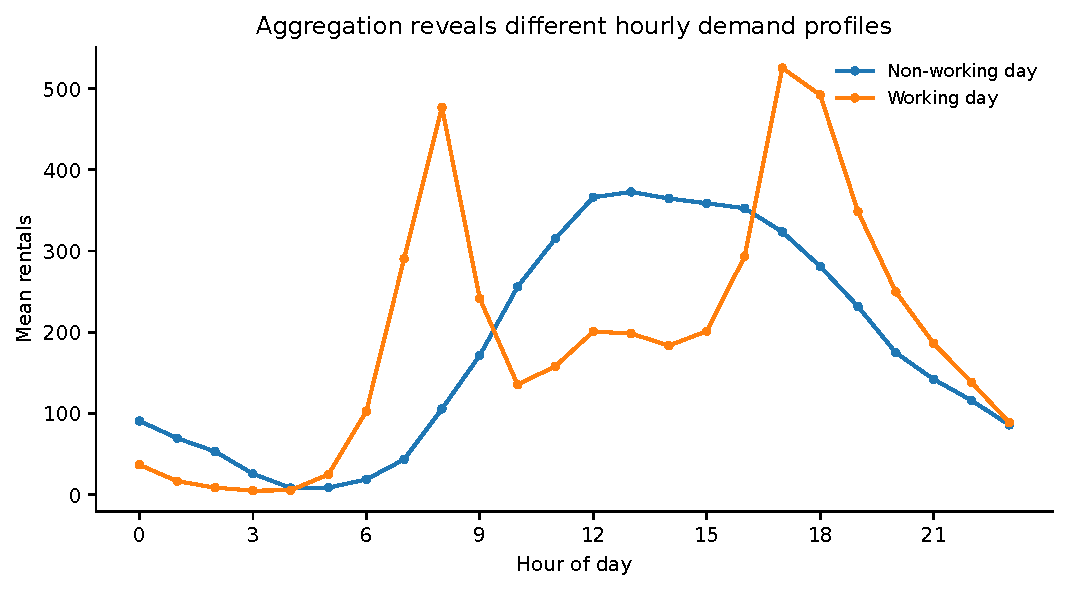
\includegraphics[width=0.86\linewidth]{figures/wrangling_bike_hourly_profiles.pdf}
\end{utpfig}

A useful feature engineering detail is that clock hour is cyclical. In ordinary numeric distance, hours 23 and 0 appear 23 units apart even though they are adjacent on the clock. A common encoding maps hour to the unit circle:
\[
  h_{\sin}=\sin(2\pi h/24), \qquad h_{\cos}=\cos(2\pi h/24).
\]
This representation preserves neighbourhood around midnight and gives models two smooth numeric variables instead of an arbitrary linear scale.

\begin{keyidea}
Every aggregation changes the unit of analysis. Before and after a \cmd{group}/\cmd{summarise} operation, state what one row represents. Many subtle data errors are actually grain errors.
\end{keyidea}

\labsection{3}{Reshape time-aware data and engineer defensible features}{sec:lab03}

\begin{labproject}{Wrangling and feature engineering: build an analysis-ready table}
\textbf{Coverage.} Chapter~\ref{ch:wrangling}.\\
\textbf{Goal.} You should be able to preserve observational grain, construct derived variables, aggregate intentionally, validate engineered features, and explain what information is lost when data are summarised.\\
\textbf{Dataset.} \texttt{bike\_sharing\_dataset\_hour.csv}.\\
\textbf{Scenario.} Hourly bike records are too granular for a manager who wants to understand commuting demand. Your task is to transform the source table into a compact, traceable analytical dataset without losing the meaning of the original measurements.

\textbf{Core workflow.}
\begin{enumerate}
  \item \textbf{State the grain.} Confirm that one row represents one observed hour on one date. Verify the date and hour ranges before any transformation.
  \item \textbf{Preserve raw variables.} Create readable day-type and hour labels as new fields rather than replacing coded source columns.
  \item \textbf{Engineer an operational feature.} Define peak-period categories with explicit hour boundaries. Explain why the chosen boundaries are analytical assumptions rather than facts stored in the data.
  \item \textbf{Represent cyclical time.} Create sine/cosine encodings for hour-of-day so that 23:00 is close to 00:00 in feature space. Verify the unit-circle identity numerically.
  \item \textbf{Aggregate for a question.} Produce mean rental profiles by hour and working-day status. State how the observational unit changes after aggregation.
  \item \textbf{Separate demand components.} Summarise \texttt{casual} and \texttt{registered} rentals by peak period and day type. Identify where the two user groups show materially different patterns.
  \item \textbf{Validate the transformation.} Check that group counts sum to the source row count, engineered categories contain no unexpected missing values, and total rentals remain consistent with their components.
\end{enumerate}

\begin{tryit}
\textbf{Extension.} Change one peak-period boundary and quantify how much the resulting group summaries change. Use the result to explain why feature engineering should be treated as a modelling decision that may require sensitivity analysis.
\end{tryit}

\tcbbreak
\lstinputlisting[style=utpr]{all_experiments/lab03_wrangling.R}
\begin{verification}
\textbf{Required evidence.} Submit the final analysis-ready column definitions, one grouped demand profile, and three validation checks. For every engineered variable, include a one-sentence definition precise enough for another analyst to reproduce it independently.

\textbf{Decision checkpoint.} Recommend one feature that should enter a future demand model and one feature that should \emph{not} be used without additional care. Justify both choices from the variable meaning and the risk of leakage or redundancy.
\end{verification}
\end{labproject}


\chapter{Exploratory Data Analysis}
\label{ch:eda}
\chapterguide
  {You should be able to prepare an analysis table and compute grouped summaries.}
  {use distribution, outlier, and relationship summaries to discover structure while separating exploration from confirmation.}

\section{EDA asks what the data are trying to tell you}
\term{Exploratory data analysis (EDA)} is a systematic search for distribution shape, unusual records, group differences, and relationships worth investigating. It is not a licence to report every pattern as a finding.

\begin{utpfig}[EDA lenses]{Move from one variable to pairs and then to conditional or multivariate structure.}{fig:eda-lenses}
\begin{tikzpicture}[x=\linewidth,y=1cm,
  lens/.style={draw=UTPBlue!65,fill=UTPPaleBlue,rounded corners=1.8mm,
    line width=0.7pt,text width=0.235\linewidth,
    minimum width=0.29\linewidth,minimum height=2.20cm,
    inner xsep=4mm,inner ysep=3mm,align=center,
    font=\scriptsize\color{UTPNavy}},
  flow/.style={-{Stealth[length=2mm,width=1.5mm]},
    line width=0.9pt,draw=UTPTeal}]
\node[lens] (u) at (0.17,0)
  {\textcolor{UTPBlue}{\textbf{01  DESCRIBE}}\\[5pt]
   {\footnotesize\textbf{UNIVARIATE}}\\[4pt]
   \textbf{One variable}\\[5pt]
   Shape, centre, and spread};
\node[lens] (b) at (0.50,0)
  {\textcolor{UTPBlue}{\textbf{02  RELATE}}\\[5pt]
   {\footnotesize\textbf{BIVARIATE}}\\[4pt]
   \textbf{Two variables}\\[5pt]
   Differences and relationships};
\node[lens,draw=UTPTeal!80,fill=UTPPaleTeal] (m) at (0.83,0)
  {\textcolor{UTPTeal}{\textbf{03  CONDITION}}\\[5pt]
   {\footnotesize\textbf{MULTIVARIATE}}\\[4pt]
   \textbf{Multiple variables}\\[5pt]
   Patterns within groups\\and joint structure};
\draw[flow] (u.east) -- (b.west);
\draw[flow] (b.east) -- (m.west);
\end{tikzpicture}
\end{utpfig}


\section{Start with shape before choosing a summary}
A mean and standard deviation are informative when the distribution is roughly symmetric and not dominated by extreme values. For skewed or multi-modal distributions, the median, quantiles, and plots often communicate structure more faithfully.

\begin{utpfig}[Three distribution shapes]{Symmetric, skewed, and bimodal distributions can require different summaries and different follow-up questions. Bimodality often suggests hidden groups or multiple data-generating processes.}{fig:eda-shapes}
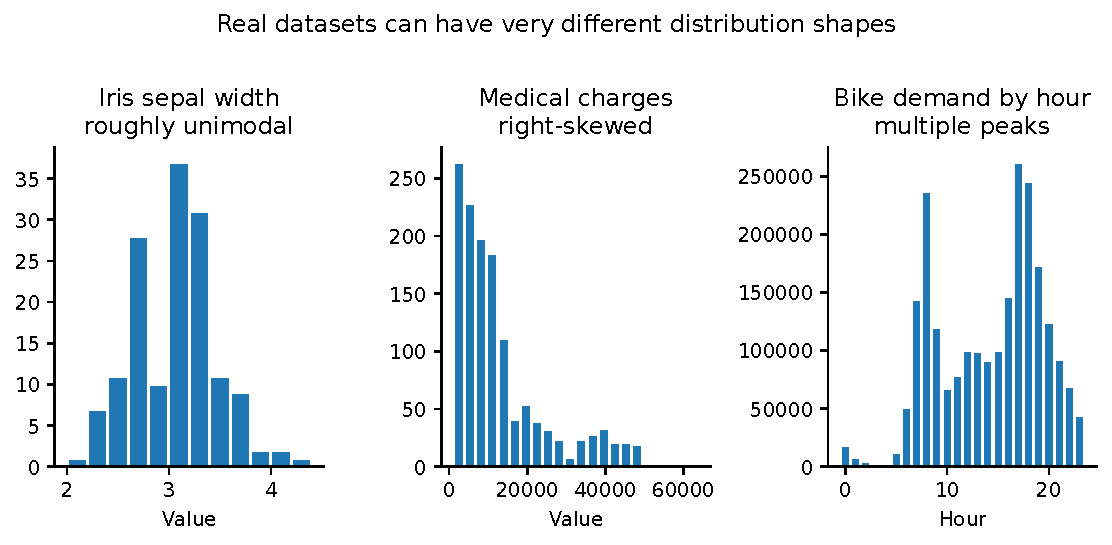
\includegraphics[width=0.90\linewidth]{figures/eda_distribution_shapes.pdf}
\end{utpfig}

A useful first pass records the minimum, lower quartile, median, upper quartile, maximum, mean, standard deviation, missing count, and sample size. The goal is not to report every number, but to notice when the numbers disagree in ways that suggest skew, extreme values, or subgroup structure.

\section{Center without spread is incomplete}
The mean is sensitive to extreme values; the median is more robust. Standard deviation describes typical distance from the mean; the interquartile range (IQR) describes the middle half of the data.

\begin{utptable}
\begin{tabularx}{\linewidth}{@{}>{\bfseries\leavevmode\color{UTPNavy}}m{4.0cm}Y>{\centering\arraybackslash}m{3.0cm}@{}}
\toprule
\rowcolor{UTPPaleBlue!92}
\utpth{Statistic} & \utpth{What it describes} & \utpth{\shortstack{Robust to\\extreme values?}} \\
\midrule
Mean & arithmetic center & no \\
Median & middle ordered value & yes \\
Standard deviation & spread around mean & no \\
IQR & spread of middle 50\% & yes \\
Range & minimum to maximum & no \\
\bottomrule
\end{tabularx}
\end{utptable}


\begin{utpfig}[Mean versus median under an outlier]{The mean shifts toward an extreme observation because every value contributes its magnitude. The median depends mainly on order and therefore moves much less.}{fig:eda-mean-median}
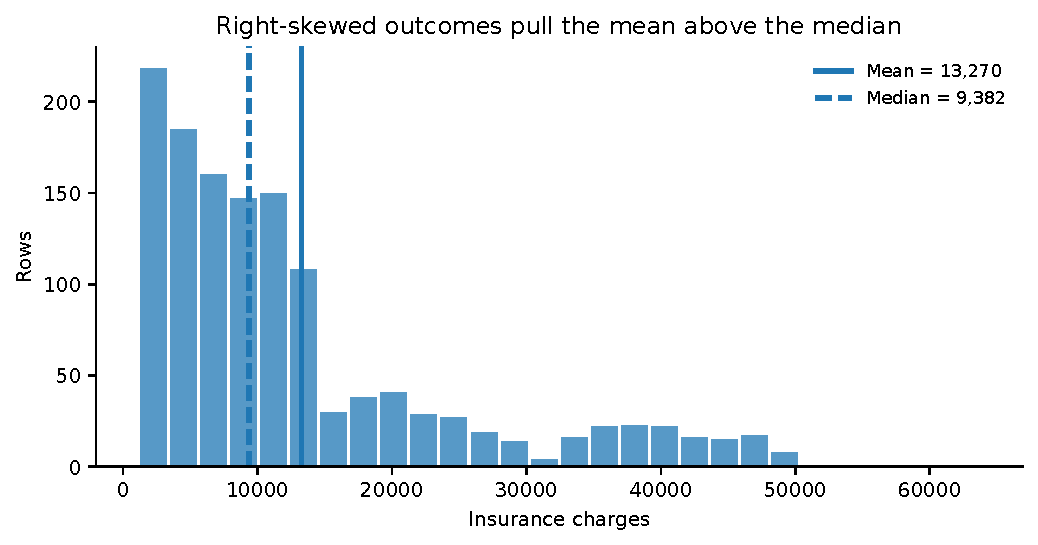
\includegraphics[width=0.84\linewidth]{figures/eda_mean_median_outlier.pdf}
\end{utpfig}

\section{Quantiles describe relative position}
The $p$th quantile is a value below which approximately $p$ proportion of observations fall. Quartiles divide ordered data into four parts; percentiles generalise the same idea. Quantiles are particularly useful for skewed variables because they describe position without assuming symmetry.


\section{Outliers are observations to investigate}
The common 1.5-IQR rule flags values outside
\[
[Q_1 - 1.5\,IQR,\; Q_3 + 1.5\,IQR].
\]
A flag is not a deletion instruction. An extreme observation may be a data error, a rare but valid case, or the most important record in the dataset.

\begin{pitfall}
Deleting outliers because they ``look wrong'' can manufacture a cleaner relationship than the population actually has. Investigate provenance and domain plausibility before removal.
\end{pitfall}


\section{Bivariate EDA depends on variable types}
Different pairs of variable types call for different evidence:
\begin{itemize}
  \item numeric--numeric: scatterplot, correlation, fitted trend, unusual points;
  \item numeric--categorical: side-by-side distributions, group medians/means and spread;
  \item categorical--categorical: contingency tables, conditional proportions, mosaic-style comparisons.
\end{itemize}
The main question is whether the second variable changes the distribution of the first, and whether that change is large enough to matter.


\section{Relationships need visual and numerical evidence}
Correlation summarizes linear association on a scale from -1 to 1. It does not establish causation and can be distorted by nonlinearity, outliers, restricted ranges, or confounding variables.


\begin{utpfig}[Correlation matrix for selected wine measurements]{The matrix summarises pairwise linear association. Strong blocks can reveal redundant features or groups of measurements that move together, but correlation alone does not identify causal relationships.}{fig:eda-corr-heatmap}
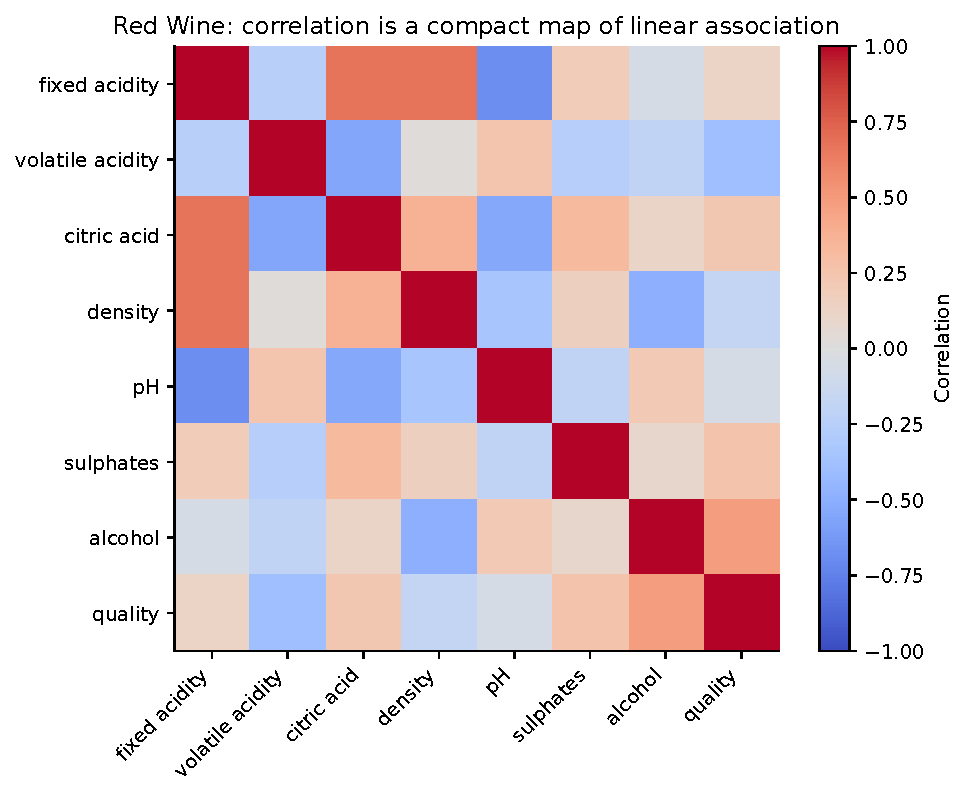
\includegraphics[width=0.74\linewidth]{figures/eda_correlation_heatmap.pdf}
\end{utpfig}

\section{Conditional patterns can reverse an overall pattern}
A relationship in aggregated data can weaken, disappear, or reverse after conditioning on a third variable. This is one reason to examine important relationships within meaningful subgroups. The phenomenon is often associated with \term{Simpson's paradox}: aggregation combines group composition with within-group relationships.

When an overall scatterplot or mean difference seems surprising, ask whether a grouping variable, time period, geography, or data-collection mechanism could be mixing distinct populations.


\begin{workedexample}
If alcohol and colour intensity are correlated in the wine data, plausible explanations include shared chemistry, cultivar differences, or another measured property. A scatterplot coloured or split by cultivar can reveal whether the overall association is partly a group effect.
\end{workedexample}

\section{Exploration versus confirmation}
EDA generates hypotheses. Confirmatory analysis evaluates a question that is sufficiently pre-specified to support formal uncertainty statements. Reusing the same dataset to discover and confirm a pattern tends to overstate certainty.

\begin{keyidea}
Write observations in evidence language: ``The median is higher in group A'' or ``the scatterplot shows a curved relationship.'' Avoid causal language unless the study design supports it.
\end{keyidea}

\section{A repeatable EDA checklist}
\begin{utpsteps}
  \item Verify row count, variable types, missingness, and plausible ranges.
  \item Examine each important numeric distribution and categorical frequency table.
  \item Compare the target or key outcome across relevant groups.
  \item Plot important numeric pairs and inspect correlations cautiously.
  \item Investigate unusual records and record any exclusions.
  \item Summarise three to five evidence-backed observations and open questions.
\end{utpsteps}

\begin{quickcheck}
\begin{enumerate}
  \item When is the median more informative than the mean?
  \item Why is an IQR outlier flag not sufficient reason to delete a row?
  \item Name two ways a correlation can be misleading.
  \item Why should exploratory and confirmatory analysis be distinguished?
\end{enumerate}
\end{quickcheck}

\section{Worked EDA: medical insurance charges}

The Medical Cost Personal dataset is useful because it contains a strongly right-skewed numeric outcome and a subgroup with a large distributional shift. It illustrates why EDA should combine distribution shape, robust summaries, and conditional comparisons.

\begin{utpfig}[Insurance charges: shape before model]{The overall distribution is right-skewed. Splitting by smoking status reveals a much larger shift than an overall histogram alone would communicate.}{fig:eda-medical-costs}
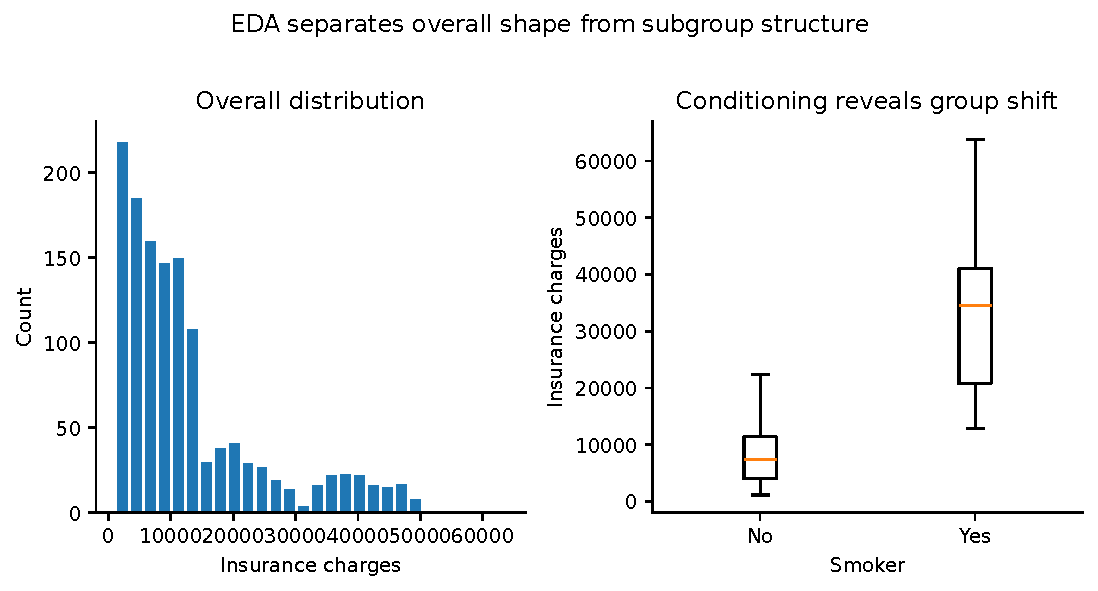
\includegraphics[width=0.90\linewidth]{figures/eda_medical_costs.pdf}
\end{utpfig}

In the bundled file, mean charges are roughly \$8,434 for non-smokers and \$32,050 for smokers; the corresponding medians are about \$7,345 and \$34,456. The difference between mean and median within each group is itself evidence about shape and tail behaviour. Meanwhile the overall BMI--charges correlation is only about 0.20, which does not imply BMI is unimportant: its association can differ by smoking status and age, and nonlinearities or interactions may matter.

\begin{pitfall}
A large group difference discovered during EDA should not be promoted directly to a causal story. Smoking status, age, BMI, and other measured or unmeasured factors are not randomly assigned in this observational dataset.
\end{pitfall}

\labsection{4}{Explore distributions, subgroups, and relationships}{sec:lab04}

\begin{labproject}{Exploratory analysis: develop a defensible EDA narrative}
\textbf{Coverage.} Chapter~\ref{ch:eda}.\\
\textbf{Goal.} You should be able to combine robust summaries and graphics, investigate subgroup structure, detect when aggregate relationships are misleading, and translate exploration into testable modelling questions.\\
\textbf{Dataset.} \texttt{medical\_cost\_personal\_dataset.csv}.\\
\textbf{Scenario.} An insurer wants to understand the structure of medical charges before any predictive model is considered. Your task is to discover patterns, identify plausible interactions, and separate observations that are unusual from observations that are invalid.

\textbf{Core workflow.}
\begin{enumerate}
  \item \textbf{Profile the target.} Describe \texttt{charges} using mean, median, quartiles, IQR, standard deviation, and a histogram. Explain what the gap between mean and median says about shape.
  \item \textbf{Flag, do not delete, extremes.} Use the $1.5\times\mathrm{IQR}$ rule to identify high-charge observations. Inspect their characteristics and explain why statistical extremeness alone is not a data-quality failure.
  \item \textbf{Compare an important subgroup.} Contrast smokers and non-smokers using group size, mean, median, spread, and a distribution plot. Decide whether the difference is large relative to within-group variability.
  \item \textbf{Check a weaker grouping variable.} Compare median charges across regions. Avoid ranking regions without considering sample size and overlap in the distributions.
  \item \textbf{Investigate a numeric relationship.} Examine BMI versus charges overall, then separately by smoking status. Compare the correlations and visible slopes.
  \item \textbf{Look for interaction.} Decide whether smoking status appears to modify the BMI--charge relationship. Express the finding as a modelling hypothesis rather than a causal claim.
  \item \textbf{Prioritise next steps.} Identify one pattern worth modelling, one variable requiring transformation or nonlinear treatment, and one plausible confounder or interaction.
\end{enumerate}

\begin{tryit}
\textbf{Extension.} Compare charges across age bands within smoking groups. Determine whether a pattern seen in the overall sample persists after conditioning on smoking status.
\end{tryit}

\tcbbreak
\lstinputlisting[style=utpr]{all_experiments/lab04_eda.R}
\begin{verification}
\textbf{Required evidence.} Submit an EDA brief containing three graphics and no more than six evidence statements. Each statement must include the comparison or relationship, its direction/magnitude, and an appropriate limitation.

\textbf{Professional standard.} Exploration is used to generate and refine hypotheses. Do not present a pattern discovered in the same data as if it were independently confirmed evidence.
\end{verification}
\end{labproject}


\chapter{Data Visualization and Communication}
\label{ch:visualization}
\chapterguide
  {You should understand distributions, grouped comparisons, outliers, and relationships.}
  {choose charts by analytical purpose; map variables to visual encodings; and write interpretations that do not overclaim.}

\section{Choose the chart from the question}
A chart is an argument made with visual encodings. The plot type should match the task rather than personal preference.

\begin{utptable}
\begin{tabularx}{\linewidth}{@{}>{\bfseries\leavevmode\color{UTPNavy}}m{4.0cm}D{4.1cm}Y@{}}
\toprule
\rowcolor{UTPPaleBlue!92}
\utpth{Analytical task} & \utpth{Useful chart} & \utpth{Read from the chart} \\
\midrule
Distribution & histogram / density / box plot & shape, center, spread, unusual values \\
Compare categories & bar chart / box plot & differences in counts or distributions \\
Numeric relationship & scatterplot & form, direction, strength, clusters, outliers \\
Change over ordered time & line chart & direction, rate, turning points \\
Part-to-whole & stacked bar (sparingly) & composition, preferably with common baselines \\
\bottomrule
\end{tabularx}
\end{utptable}

\section{Position is usually the strongest encoding}
Humans compare positions along a common axis more accurately than angles, areas, or 3D volumes. That is why a bar chart is often easier to read than a pie chart and why decorative 3D effects are rarely useful.

\begin{utpfig}[Visual encoding hierarchy]{Prefer encodings that support precise comparison when the analytical goal depends on small differences.}{fig:encoding-hierarchy}
\begin{tikzpicture}[x=\linewidth,y=1cm,
  encoding/.style={draw=UTPBlue!65,fill=UTPPaleBlue,rounded corners=1.8mm,
    line width=0.7pt,text width=0.14\linewidth,
    minimum width=0.18\linewidth,minimum height=1.70cm,
    inner xsep=2.5mm,inner ysep=2.5mm,align=center,
    font=\scriptsize\color{UTPNavy}},
  precision/.style={-{Stealth[length=2.2mm,width=1.6mm]},
    line width=1.0pt,draw=UTPTeal}]
\node[encoding,draw=UTPTeal!80,fill=UTPPaleTeal] (p) at (0.10,0)
  {\textcolor{UTPTeal}{\textbf{01}}\\[4pt]
   \textbf{POSITION}\\[5pt]
   Location on a\\common axis};
\node[encoding] (l) at (0.30,0)
  {\textcolor{UTPBlue}{\textbf{02}}\\[4pt]
   \textbf{LENGTH}\\[5pt]
   Extent along\\one dimension};
\node[encoding] (a) at (0.50,0)
  {\textcolor{UTPBlue}{\textbf{03}}\\[4pt]
   \textbf{ANGLE / SLOPE}\\[5pt]
   Angle or\\inclination};
\node[encoding] (ar) at (0.70,0)
  {\textcolor{UTPBlue}{\textbf{04}}\\[4pt]
   \textbf{AREA}\\[5pt]
   Size in\\two dimensions};
\node[encoding,draw=UTPOrange!75,fill=UTPPaleOrange] (c) at (0.90,0)
  {\textcolor{UTPOrange!85!black}{\textbf{05}}\\[4pt]
   \textbf{COLOUR}\\[5pt]
   Variation in\\intensity};
\draw[precision] (0.08,-1.12) -- (0.92,-1.12);
\foreach \x in {0.10,0.30,0.50,0.70,0.90}
  \draw[draw=UTPMuted!75,line width=0.65pt]
    (\x,-1.04) -- (\x,-1.20);
\node[anchor=north west,font=\scriptsize\bfseries\color{UTPTeal}]
  at (0.08,-1.27) {HIGHER PRECISION};
\node[anchor=north east,font=\scriptsize\bfseries\color{UTPOrange!85!black}]
  at (0.92,-1.27) {LOWER PRECISION};
\end{tikzpicture}
\end{utpfig}


\section{Every visual encoding consumes attention}
A chart encodes variables using position, length, colour, shape, size, angle, and sometimes texture. More encodings are not automatically better. Use the strongest channels for the variables most central to the question, and reserve colour or shape for secondary grouping only when it clarifies interpretation.

Direct labels, meaningful axis titles, and a descriptive caption often improve comprehension more than additional decoration. A chart should be understandable without requiring the reader to reverse-engineer arbitrary abbreviations.


\section{Histograms answer distribution questions}
Histogram appearance depends on bin boundaries. Too few bins hide structure; too many amplify noise. Use the chart to understand shape, then check conclusions across reasonable bin choices.

\begin{lstlisting}[style=utpr]
hist(wine$alcohol,
     breaks = 12,
     xlab = "Alcohol",
     main = "Distribution of alcohol measurements")
\end{lstlisting}


\begin{utpfig}[Histogram binning changes the visible story]{All three panels contain the same alcohol measurements. Few bins hide local structure; many bins can make random sample noise look important.}{fig:viz-bin-choice}
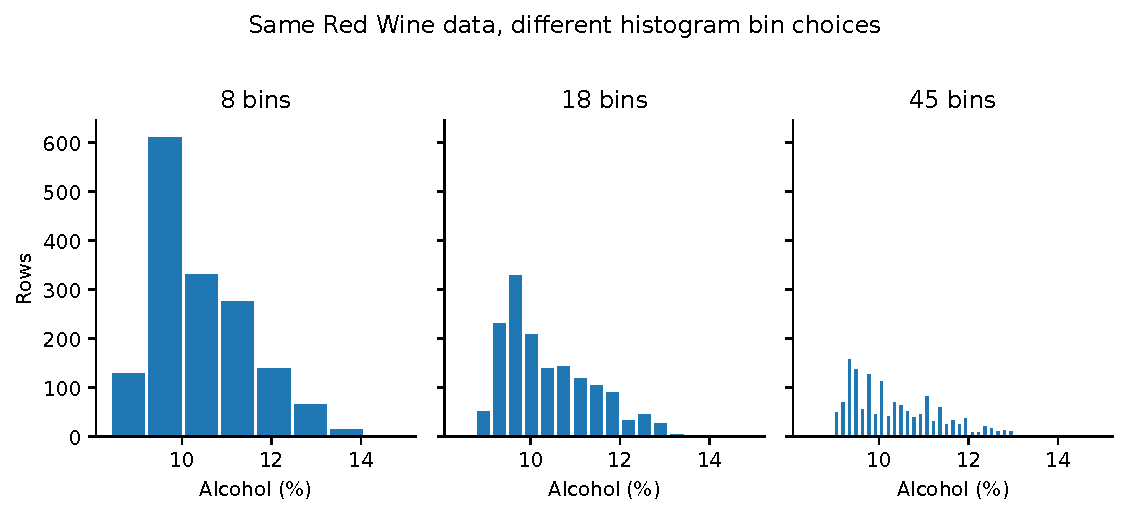
\includegraphics[width=0.91\linewidth]{figures/viz_histogram_bins.pdf}
\end{utpfig}

\section{Density, box, and violin-style views answer different questions}
A histogram or density estimate emphasises shape. A box plot emphasises median, quartiles, and outlier flags. A violin plot combines a density-like shape with a group comparison, but can suggest more precision than the sample supports when groups are small. Choose the representation that exposes the property the reader needs to compare.


\section{Box plots compare distributions compactly}
A box plot shows the median, quartiles, and potential outliers. It is effective for comparing several groups, but it hides detailed shape and sample-size differences unless additional context is provided.


\begin{utpfig}[Compact group comparison]{The same measurement can have overlapping but distinct group distributions. Box plots make medians and spread easy to compare, while the chapter's scatterplot will show within-group relationships.}{fig:viz-boxplot}
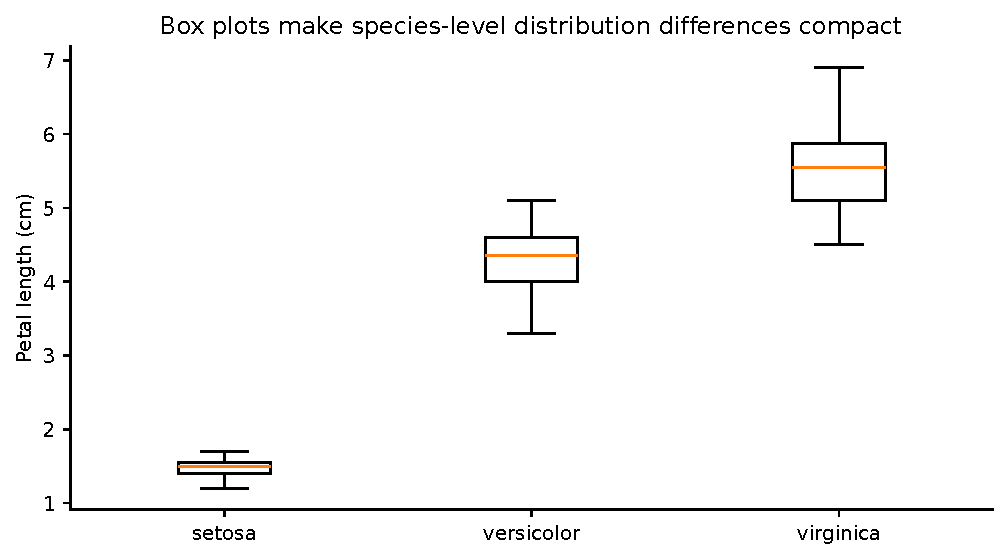
\includegraphics[width=0.77\linewidth]{figures/viz_boxplot_species.pdf}
\end{utpfig}


\section{Scatterplots are the default for two numeric variables}
A scatterplot can reveal linear or curved relationships, changing variance, distinct clusters, and influential points that one correlation coefficient cannot show.


\begin{utpfig}[Scatterplots reveal structure hidden by one coefficient]{Petal length and width have a strong overall relationship, but colour reveals three species-level groups and different local ranges.}{fig:viz-iris-scatter}
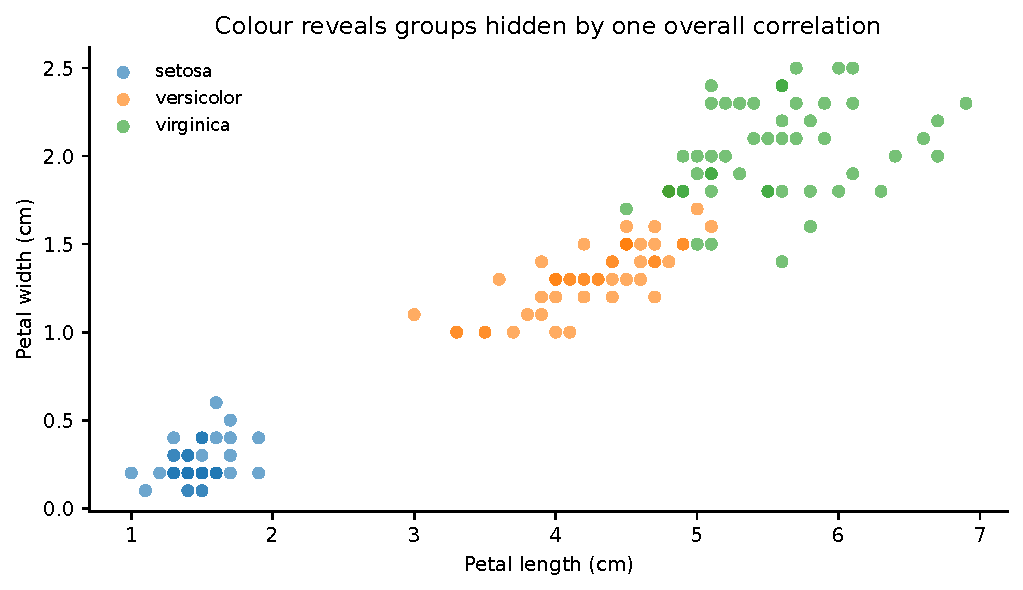
\includegraphics[width=0.76\linewidth]{figures/viz_iris_scatter.pdf}
\end{utpfig}

\section{Uncertainty should be visible when the claim is uncertain}
If a figure shows an estimated mean, fitted line, or model prediction, include an interval, error bar, distribution of resampled estimates, or another appropriate uncertainty display when possible. Showing only the point estimate can make an uncertain result appear exact.

\section{Design for comparison}
Good chart design places the values that need comparison on a common scale and close enough to compare. Small multiples are effective when several groups or time periods share the same axes. Sorting categories by a meaningful quantity can also reduce the mental work needed to find patterns.


\begin{pitfall}
Axis limits can exaggerate or conceal differences. Truncating a bar chart away from zero changes the perceived ratio of bar lengths; clipping a scatterplot can hide records that contradict the intended story. State and justify unusual scales.
\end{pitfall}

\section{A chart needs an evidence sentence}
Every figure should support a short interpretation that names the variables, describes the visible pattern, and separates observation from explanation.

\begin{workedexample}
Weak: ``The graph shows a relationship.''

Better: ``Petal length and petal width increase together, and the observations form visible species-level clusters. The plot establishes association and separation, not a biological causal mechanism.''
\end{workedexample}

\begin{keyidea}
Good visualisation reduces the distance between data and judgment. Remove decoration that does not encode information; keep labels, units, and context that make the evidence interpretable.
\end{keyidea}


\section{A visualisation review checklist}
Before publishing a chart, ask: Is the analytical question visible? Are units and population clear? Does the geometry match the variable type? Are scales honest and comparable? Is colour necessary and distinguishable? Are missing values or excluded groups acknowledged? Does the caption state the evidence rather than merely repeat the title? Could a reader misinterpret association as causation?


\begin{quickcheck}
\begin{enumerate}
  \item Why is position on a common axis easier to compare than area?
  \item What can a scatterplot reveal that correlation alone cannot?
  \item Why should histogram conclusions be checked across reasonable bin widths?
  \item What makes an interpretation sentence stronger than a chart title alone?
\end{enumerate}
\end{quickcheck}

\section{Worked visual design: red-wine quality}

The Red Wine Quality dataset contains 1,599 wines and an ordered quality score from 3 to 8. The outcome is numeric in storage but conceptually discrete and ordinal. That distinction affects chart design.

\begin{utpfig}[Alcohol content across ordered quality scores]{Boxplots preserve the discreteness of the quality score while showing a systematic shift in the alcohol distribution. The figure supports comparison without pretending that every one-unit quality change is exactly equivalent.}{fig:viz-redwine-alcohol}
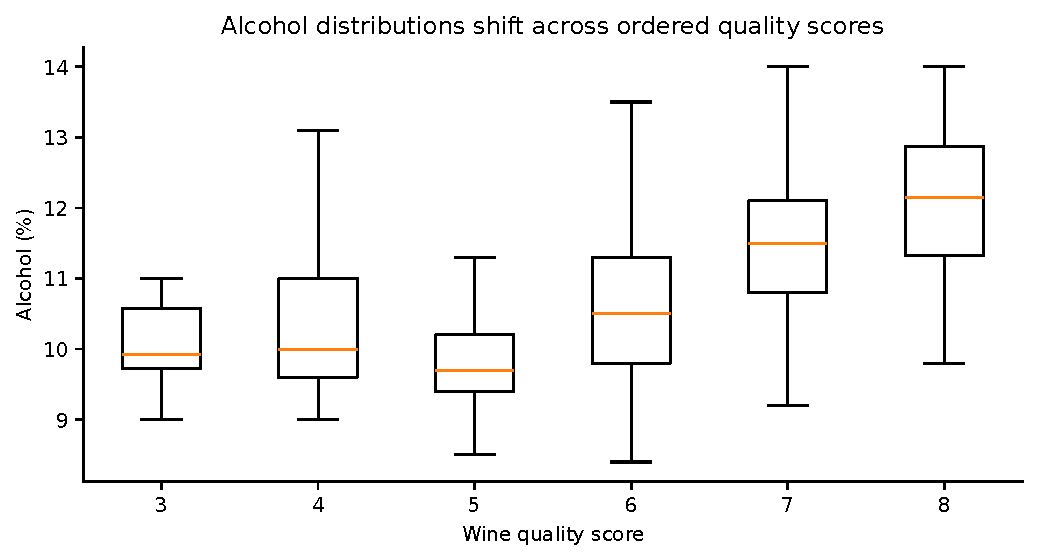
\includegraphics[width=0.82\linewidth]{figures/viz_wine_quality_alcohol.pdf}
\end{utpfig}

The correlation between alcohol and quality is about 0.48, but the boxplots communicate more: the quality groups overlap substantially and sample sizes are very unequal. Scores 5 and 6 dominate the dataset, whereas extreme scores are rare. A regression line alone would hide both facts.

\begin{keyidea}
The best chart is not the chart with the most aesthetics. It is the chart whose visual encoding makes the comparison required by the question easy and honest.
\end{keyidea}


\section{A second visual-design case: when two discrete dimensions interact}

The Bike Sharing hourly table contains two discrete coordinates that are easy to lose in a sequence of separate bar charts: hour of day and weekday. A heatmap uses position in two dimensions and colour for mean demand, allowing the reader to scan for recurring temporal structure.

\begin{utpfig}[Bike demand varies jointly by hour and weekday]{The heatmap makes morning/evening weekday peaks and broader weekend daytime use visible in one compact display. A one-dimensional average by hour would blur some of this structure.}{fig:viz-bike-heatmap}
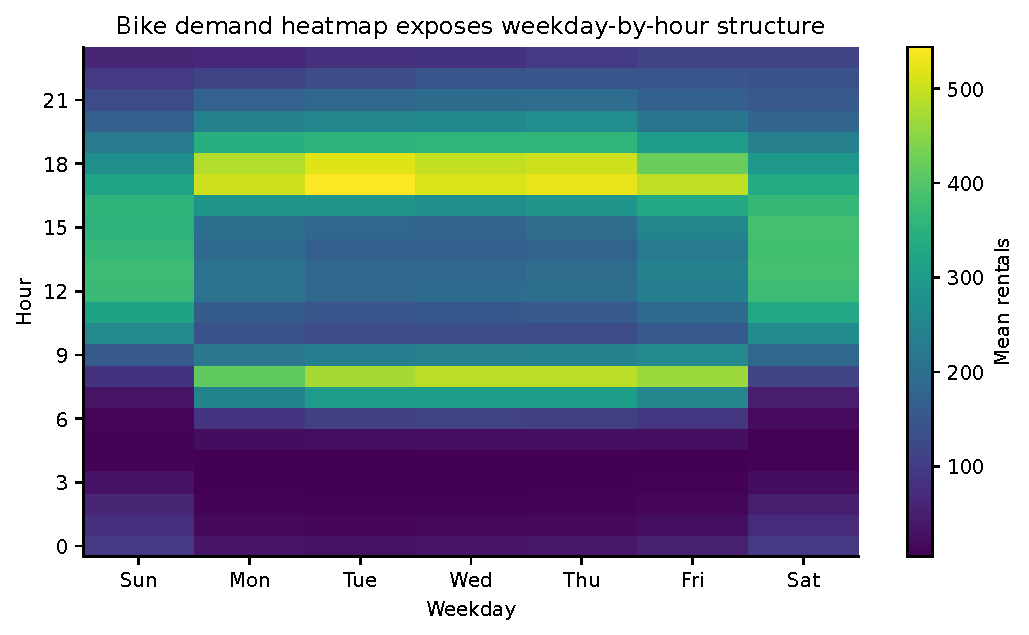
\includegraphics[width=0.80\linewidth]{figures/viz_bike_heatmap.pdf}
\end{utpfig}

This example also illustrates a design principle: aggregation should match the visual question. Each cell is a mean across many observed hours. The chart is therefore suitable for a recurring pattern, but not for showing day-to-day volatility, weather shocks, or uncertainty around each cell. A professional report should not ask one graphic to answer all of those questions simultaneously.

\labsection{5}{Design graphics that answer a question}{sec:lab05}

\begin{labproject}{Visual communication: turn analysis into evidence}
\textbf{Coverage.} Chapter~\ref{ch:visualization}.\\
\textbf{Goal.} You should be able to map analytical questions to chart forms, identify misleading encodings, write evidence-focused captions, and distinguish information revealed by raw and aggregated views.\\
\textbf{Datasets.} \texttt{red\_wine\_quality\_dataset.csv}; Bike Sharing hourly data are used for the extension.\\
\textbf{Scenario.} You are preparing figures for an analytical report. The objective is not decoration: each chart must answer a specific question, use an appropriate visual encoding, and make the intended comparison easy to see.

\textbf{Core design tasks.}
\begin{enumerate}
  \item \textbf{Distribution question.} Use a bar chart to show the frequency of the discrete wine-quality scores. Explain why a histogram is not the clearest default for this variable.
  \item \textbf{Group-comparison question.} Use side-by-side boxplots to compare alcohol content across quality scores. Support the figure with grouped numerical summaries.
  \item \textbf{Relationship question.} Use a scatterplot to examine volatile acidity and alcohol. Describe what can and cannot be inferred when neither variable is an outcome in the graphic.
  \item \textbf{Redesign by changing the question.} Create a second version of one figure that answers a genuinely different analytical question. Do not count changes in colour, font, or theme as a redesign.
  \item \textbf{Write analytical captions.} For each figure, state the data subset, visual encoding, main visible pattern, and one limitation or uncertainty.
  \item \textbf{Perform a visual integrity check.} Identify one choice that would exaggerate, hide, or confuse the pattern---for example, an inappropriate axis, unnecessary 3-D effect, excessive overplotting, or treating a discrete score as continuous without explanation.
\end{enumerate}

\begin{tryit}
\textbf{Extension---two-dimensional time structure.} Use \texttt{bike\_sharing\_dataset\_hour.csv} to create an hour-by-weekday heatmap of mean rentals. Explain what the heatmap reveals about commuting structure that a single hourly line cannot, and identify what variability is hidden by averaging.
\end{tryit}

\tcbbreak
\lstinputlisting[style=utpr]{all_experiments/lab05_visualization.R}
\begin{verification}
\textbf{Required evidence.} Submit a three-figure mini-report. Each figure must have a one-sentence question above it and a two-to-three sentence evidence caption below it. A reader should understand the analytical claim without seeing the R code.

\textbf{Professional standard.} Prefer the simplest chart that makes the required comparison accurately. Visual complexity is justified only when it reveals additional structure.
\end{verification}
\end{labproject}



\part{Uncertainty and Predictive Modelling}
\chapter{Sampling, Uncertainty, and Statistical Inference}
\label{ch:inference}
\chapterguide
  {You should be comfortable with descriptive statistics, distributions, and group comparisons.}
  {distinguish population from sample, explain sampling variability, construct bootstrap confidence intervals, and interpret hypothesis tests alongside effect size.}

\section{A sample is one possible view of a population}
A \term{population} is the set of cases the question concerns. A \term{sample} is the observed subset. Statistics computed from a sample vary from sample to sample, even when the underlying population is unchanged.

\begin{utpfig}[Sampling variability]{Different random samples produce different estimates. Statistical inference quantifies that uncertainty rather than pretending the observed sample is exact.}{fig:sampling-variability}
\begin{tikzpicture}[x=\linewidth,y=1cm,
  card/.style={draw=UTPBlue!70,fill=UTPPaleBlue,rounded corners=1.5mm,
    line width=0.6pt,text width=0.26\linewidth,minimum height=1.45cm,
    inner xsep=2.5mm,inner ysep=2mm,align=center,
    font=\scriptsize\color{UTPNavy}},
  connector/.style={line width=0.8pt,draw=UTPTeal,rounded corners=1.5mm},
  flow/.style={connector,-{Stealth[length=2mm,width=1.5mm]}}]
\node[card] (pop) at (0,0) {\textbf{Population}\\[4pt]
  Cases of interest\\Unknown parameter};
\node[card] (s1) at (0.335,1.05) {\textbf{Sample A}\\[4pt]
  Observed subset\\Estimate A};
\node[card] (s2) at (0.335,-1.05) {\textbf{Sample B}\\[4pt]
  Observed subset\\Estimate B};
\node[card,draw=UTPTeal!80,fill=UTPPaleTeal] (dist) at (0.670,0)
  {\textbf{Sampling distribution}\\[4pt]
   Estimates across samples\\Sampling uncertainty};
\coordinate (split) at (0.1675,0);
\coordinate (merge) at (0.5025,0);
\draw[connector] (pop.east) -- (split);
\draw[flow] (split) |- (s1.west);
\draw[flow] (split) |- (s2.west);
\draw[connector] (s1.east) -| (merge);
\draw[connector] (s2.east) -| (merge);
\draw[flow] (merge) -- (dist.west);
\node[font=\scriptsize\color{UTPMuted},align=center,
  text width=0.30\linewidth] at (0.335,2.05)
  {Illustrative repeated samples};
\end{tikzpicture}
\end{utpfig}


\begin{utpfig}[Sampling distribution of a mean]{Each simulated point in the histogram is a mean from a sample of 30 wine observations. The means vary from sample to sample but are more concentrated than individual measurements.}{fig:inference-sampling-dist}
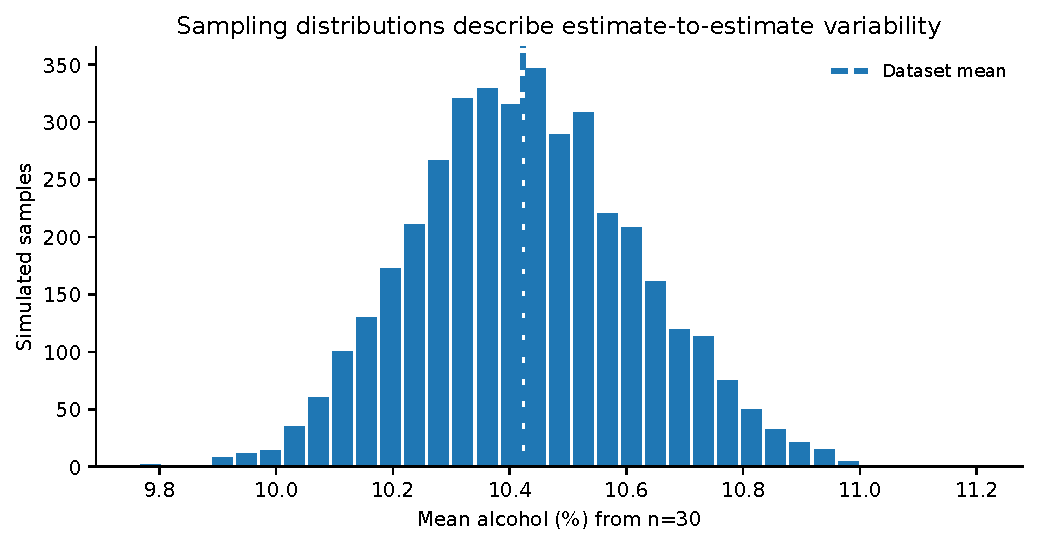
\includegraphics[width=0.84\linewidth]{figures/inference_sampling_distribution.pdf}
\end{utpfig}

\section{Standard error describes estimate-to-estimate variability}
The \term{standard error} is the standard deviation of a statistic's sampling distribution. For a sample mean under familiar assumptions,
\[
SE(\bar{x}) \approx \frac{s}{\sqrt{n}}.
\]
The square-root relationship is important: quadrupling sample size roughly halves the standard error, all else equal. This gain in precision does not remove bias from poor sampling or measurement.


\section{Bias and variability are different problems}
A large convenience sample can estimate the wrong population very precisely. More observations reduce random variability, but they do not automatically repair selection bias, measurement bias, or confounding.

\section{Bootstrap confidence intervals}
The bootstrap approximates sampling variability by repeatedly resampling the observed data with replacement.

\begin{utpsteps}
  \item Compute the statistic of interest on the observed sample.
  \item Resample the rows with replacement to create a bootstrap sample of the same size.
  \item Recompute the statistic and store it.
  \item Repeat many times; use the bootstrap distribution to form an interval.
\end{utpsteps}

\begin{lstlisting}[style=utpr]
set.seed(42)
boot_means <- replicate(
  2000,
  mean(sample(wine$alcohol, replace = TRUE))
)
quantile(boot_means, c(0.025, 0.975))
\end{lstlisting}


\begin{utpfig}[Bootstrap distribution]{Bootstrap resamples mimic repeated sampling from an empirical approximation to the population. The central 95\% of the resampled means gives a simple percentile interval.}{fig:inference-bootstrap}
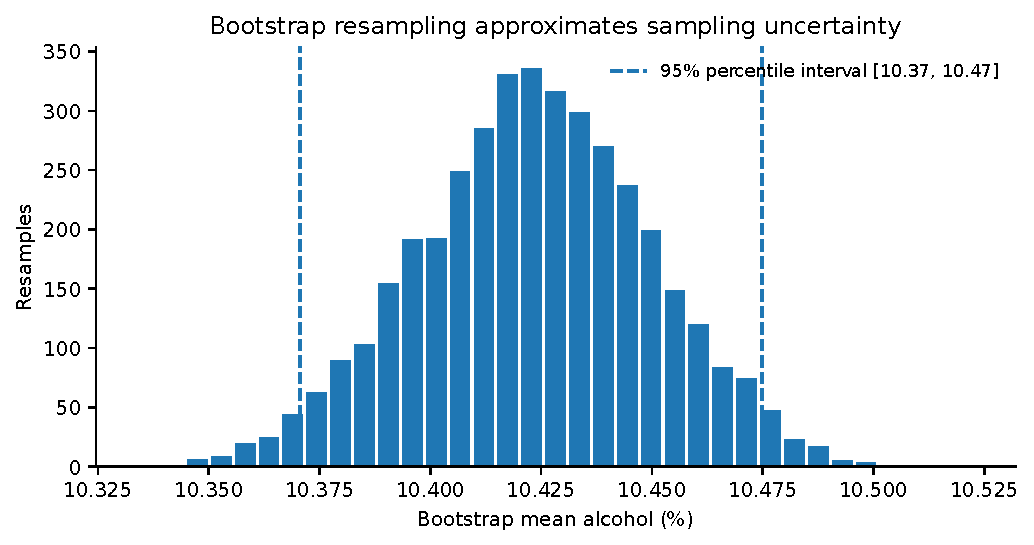
\includegraphics[width=0.84\linewidth]{figures/inference_bootstrap.pdf}
\end{utpfig}

\section{Confidence intervals quantify a range of compatible values}
A 95\% confidence interval is produced by a procedure designed to cover the target parameter about 95\% of the time under repeated sampling and the method's assumptions. Once a particular interval has been calculated, the parameter is fixed; the frequentist interpretation concerns the long-run procedure rather than a 95\% probability assigned to that fixed parameter.

\begin{utpfig}[Repeated-sampling interpretation of confidence intervals]{Most intervals in this simulation cross the dashed population mean; occasional intervals miss it. This long-run behaviour is what confidence level describes.}{fig:inference-ci-coverage}
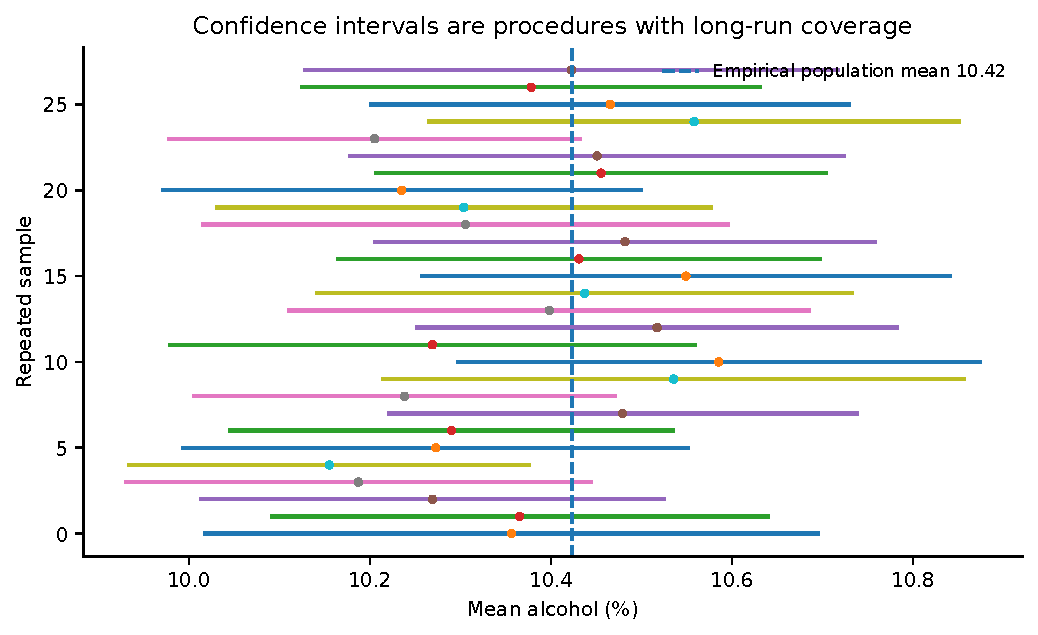
\includegraphics[width=0.82\linewidth]{figures/inference_ci_repeated.pdf}
\end{utpfig}

\section{Hypothesis tests compare data with a null model}
A p-value is the probability, under a specified null hypothesis and test assumptions, of obtaining a result at least as incompatible with the null as the observed result. It is not the probability that the null hypothesis is true.

\begin{pitfall}
``Statistically significant'' does not mean ``important'', ``large'', or ``causal''. With enough data, a tiny difference can have a small p-value. Always report the magnitude and practical meaning of the effect.
\end{pitfall}


\section{A hypothesis test has several moving parts}
A disciplined test states the null and alternative hypotheses, chooses a statistic, checks assumptions, computes the statistic's null reference distribution or approximation, and then interprets the p-value in context. The p-value is sensitive to both effect size and sample size, which is why it should not be used as a stand-alone measure of scientific importance.

For a two-group comparison, also inspect group distributions and report an effect such as a difference in means or medians in original units. If a standardised effect size is useful for comparison across scales, explain what its units mean.


\section{Effect size and uncertainty belong together}
For a difference in means, report the observed difference in original units and an interval or test that describes uncertainty. Readers can then judge both size and precision.

\begin{workedexample}
Suppose two wine cultivars differ in mean alcohol measurement. The t-test addresses compatibility with a zero-difference model; the actual difference in alcohol units tells the reader whether the magnitude is meaningful in context.
\end{workedexample}


\section{Multiple testing increases false discoveries}
If an analyst tests many unrelated hypotheses and reports only those with small p-values, some apparently ``significant'' results can arise by chance. Pre-specifying primary questions, correcting for multiplicity when appropriate, and validating exploratory findings on new data reduce this risk.

\begin{pitfall}
A confidence interval or p-value quantifies uncertainty conditional on assumptions. It does not automatically account for selection bias, measurement error, poor operational definitions, unrecorded exclusions, or the fact that the hypothesis was chosen after inspecting the same data.
\end{pitfall}


\section{Study design limits causal claims}
Randomised experiments can isolate treatment effects when implemented well. Observational data can describe associations and support prediction, but causal interpretation requires stronger assumptions and methods than correlation or regression alone.

\begin{keyidea}
Inference is not a machine for turning samples into certainty. It is a framework for expressing what the data say while keeping sampling and design uncertainty visible.
\end{keyidea}

\begin{quickcheck}
\begin{enumerate}
  \item What is the difference between sampling variability and selection bias?
  \item What does resampling with replacement accomplish in the bootstrap?
  \item What does a p-value \emph{not} tell you?
  \item Why should effect size accompany statistical significance?
\end{enumerate}
\end{quickcheck}

\section{Worked inference: student performance and observational uncertainty}

In the Student Performance dataset, mean final grade \texttt{G3} is about 12.28 among students who report an intention to pursue higher education and about 8.80 among those who do not---an observed difference of roughly 3.48 grade points.

\begin{utpfig}[Bootstrap distribution for a mean difference]{Resampling students within the observed groups approximates the sampling variability of the group mean difference under the empirical distribution. The interval describes uncertainty in the estimate, not uncertainty about unmeasured confounding.}{fig:inference-student-bootstrap}
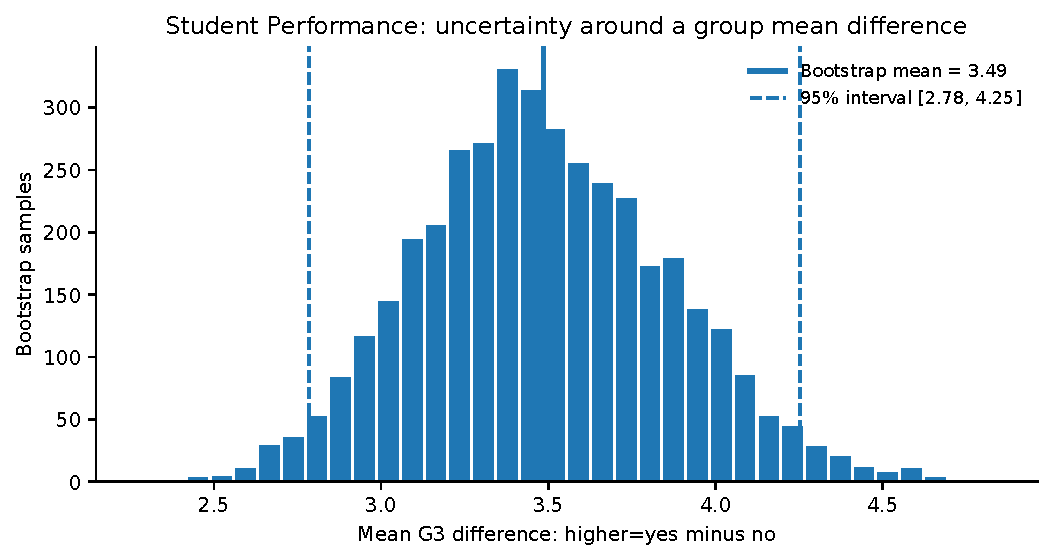
\includegraphics[width=0.86\linewidth]{figures/inference_student_bootstrap.pdf}
\end{utpfig}

This example separates three questions that students often merge. \textbf{Estimation} asks how large the observed difference is. \textbf{Sampling uncertainty} asks how much that estimate might vary under repeated sampling. \textbf{Causal interpretation} asks whether changing higher-education intention would change grades. Bootstrap intervals help with the second question; they do not solve the third.

Potential confounders include prior grades, study time, parental education, school support, failures, and socioeconomic context. Formal uncertainty can be numerically precise while the causal claim remains weak.


\section{Bootstrap and permutation answer different questions}

The Student Performance example is useful because two resampling procedures can be placed side by side. The bootstrap resamples within the observed groups and asks how much the estimated mean difference would vary if similar samples were collected again. A permutation procedure instead breaks the link between group label and outcome and asks how unusual the observed contrast is under an exchangeability-based no-association reference model.

\begin{utpfig}[Permutation inference creates a null reference distribution]{The shuffled-label distribution is centred near zero because the group labels have been deliberately detached from final grades. The observed difference is then compared with this reference distribution.}{fig:inference-student-permutation}
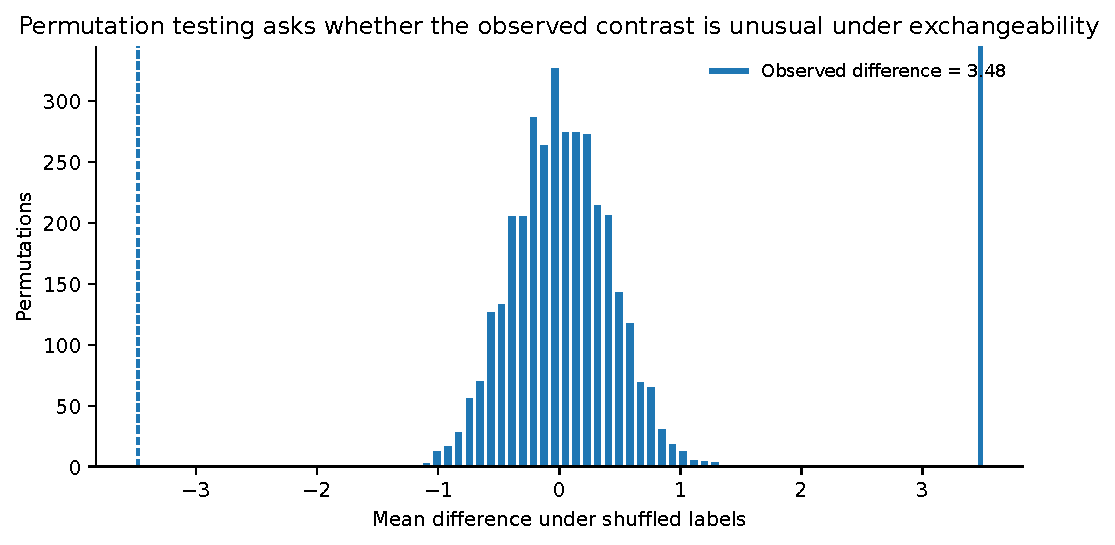
\includegraphics[width=0.82\linewidth]{figures/inference_student_permutation.pdf}
\end{utpfig}

The procedures are related but not interchangeable. The bootstrap is primarily an estimation tool here; the permutation distribution is a testing tool. Both inherit assumptions from the sampling process, and neither makes the observational comparison causal. This is why a complete inference statement should report the \textbf{effect size}, the \textbf{uncertainty or reference distribution}, and the \textbf{design limitation} in separate sentences.

\labsection{6}{Quantify uncertainty with bootstrap and permutation logic}{sec:lab06}

\begin{labproject}{Sampling and inference: estimate, quantify, challenge}
\textbf{Coverage.} Chapter~\ref{ch:inference}.\\
\textbf{Goal.} You should be able to define an estimand, construct a bootstrap interval, build a permutation reference distribution, report effect size, and separate statistical evidence from study-design limitations.\\
\textbf{Dataset.} \texttt{student\_performance\_dataset.csv}.\\
\textbf{Scenario.} A school analyst observes a grade difference between students who report intending higher education and those who do not. Your task is to quantify the difference, assess sampling uncertainty, and prevent statistical significance from being mistaken for a causal conclusion.

\textbf{Core workflow.}
\begin{enumerate}
  \item \textbf{Define the estimand.} Let the target be the difference in mean final grade \texttt{G3} between \texttt{higher=yes} and \texttt{higher=no}. Report group sizes and descriptive summaries before inference.
  \item \textbf{Estimate the observed effect.} Compute the mean difference and a standardised difference. Interpret direction and practical size in the units of the problem.
  \item \textbf{Bootstrap uncertainty.} Resample within groups, generate at least 5,000 bootstrap estimates, and construct a 95\% percentile interval for the mean difference.
  \item \textbf{Construct a null model.} Permute the group labels while keeping grades fixed. Use the resulting distribution to estimate a two-sided p-value for no group association.
  \item \textbf{Compare inferential quantities.} Explain what the point estimate, confidence interval, standardised effect, and p-value each contribute. Explicitly state what none of them establishes.
  \item \textbf{Audit design limitations.} Identify at least three available variables that may confound the association, such as prior grades, failures, study time, family education, or absences.
  \item \textbf{Write a defensible conclusion.} Separate the statistical conclusion from the causal conclusion in two distinct sentences.
\end{enumerate}

\begin{tryit}
\textbf{Extension.} Repeat the comparison after stratifying or adjusting descriptively for one plausible confounder. Do not claim that this single adjustment removes confounding; use it as a sensitivity check on the original result.
\end{tryit}

\tcbbreak
\lstinputlisting[style=utpr]{all_experiments/lab06_inference.R}
\begin{verification}
\textbf{Required evidence.} Submit the observed effect, 95\% interval, permutation p-value, one bootstrap distribution graphic, and a four-sentence interpretation covering magnitude, uncertainty, null evidence, and design limitation.

\textbf{Professional standard.} Report uncertainty and effect size together. A small p-value without a meaningful effect estimate is not a complete scientific result.
\end{verification}
\end{labproject}


\chapter{Regression for Numeric Prediction}
\label{ch:regression}
\chapterguide
  {You should understand relationships, sampling uncertainty, and the difference between exploration and validation.}
  {fit a multiple linear regression, interpret coefficients cautiously, evaluate predictions on held-out data, and diagnose residual errors.}

\section{Regression predicts a numeric target}
In supervised learning, the dataset includes an outcome to be predicted. \term{Regression} is used when that target is numeric, such as price, demand, temperature, or concentration.

A multiple linear model has the form
\[
\hat{y}=\beta_0 + \beta_1x_1 + \cdots + \beta_px_p.
\]
The coefficients describe modelled changes in the prediction while holding the other included features fixed. That is not automatically a causal effect.


\section{What a fitted line is minimising}
Ordinary least squares chooses coefficients to minimise the sum of squared residuals. In a one-feature model, each residual is the vertical difference between the observed target and the fitted line.

\begin{utpfig}[Regression geometry and residuals]{The vertical segments are residuals. Squaring them makes large errors contribute disproportionately to the least-squares objective.}{fig:regression-geometry}
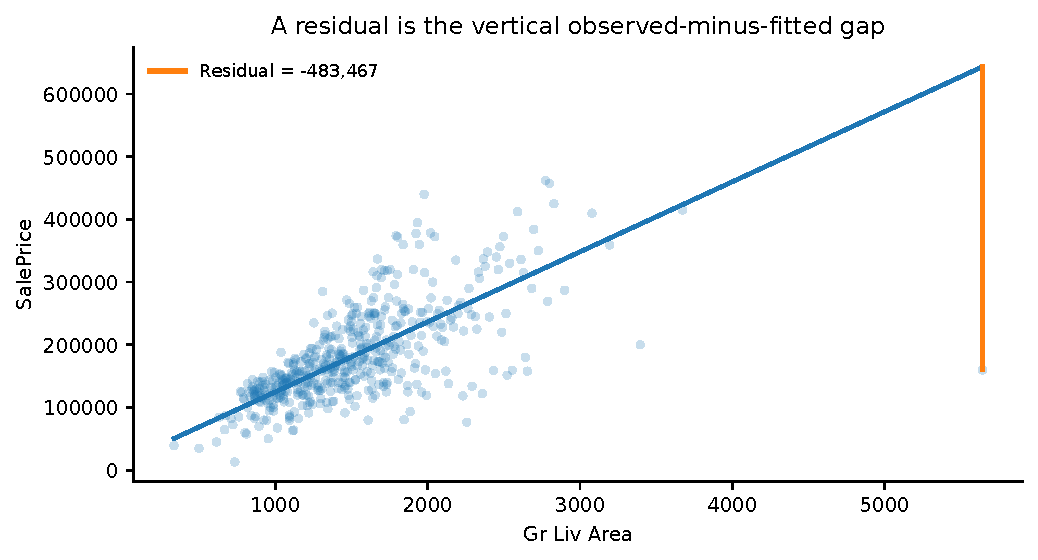
\includegraphics[width=0.80\linewidth]{figures/regression_residual_geometry.pdf}
\end{utpfig}

In multiple regression, the geometry lives in higher-dimensional feature space, but the interpretation is similar: predictions are linear combinations of the included features and residuals measure unexplained target variation.


\section{Training error is not enough}
A flexible model can fit patterns specific to the observed sample. To evaluate generalisation, split the data so some observations are not used to fit the model.

\begin{utpfig}[Train/test workflow]{Model parameters are learned from the training set. The test set is touched only after the model and preprocessing choices are fixed.}{fig:train-test-regression}
\begin{tikzpicture}[x=\linewidth,y=1cm,
  card/.style={draw=UTPBlue!65,fill=UTPPaleBlue,rounded corners=1.8mm,
    line width=0.7pt,text width=0.27\linewidth,
    minimum width=0.34\linewidth,minimum height=1.18cm,
    inner xsep=4mm,inner ysep=2mm,align=center,
    font=\scriptsize\color{UTPNavy}},
  flow/.style={-{Stealth[length=2.2mm,width=1.6mm]},
    line width=0.9pt,draw=UTPTeal},
  testflow/.style={-{Stealth[length=2.2mm,width=1.6mm]},
    line width=0.9pt,draw=UTPOrange!85!black},
  targetflow/.style={-{Stealth[length=2.2mm,width=1.6mm]},
    line width=0.8pt,draw=UTPOrange!85!black,dashed},
  flowlabel/.style={fill=white,rounded corners=1mm,
    inner xsep=2.5mm,inner ysep=1mm,
    font=\tiny\bfseries}]
\node[card,draw=UTPTeal!80,fill=UTPPaleTeal] (all) at (0.50,4.20)
  {\textcolor{UTPTeal}{\textbf{01  AVAILABLE DATA}}\\[4pt]
   Features and target\\before splitting};
\node[card] (train) at (0.28,0.85)
  {\textcolor{UTPBlue}{\textbf{02A  TRAINING PARTITION}}\\[4pt]
   Used to learn\\model parameters};
\node[card,draw=UTPOrange!80,fill=UTPPaleOrange] (test) at (0.72,0.85)
  {\textcolor{UTPOrange!85!black}{\textbf{02B  TEST PARTITION}}\\[4pt]
   Held out from\\model fitting};
\node[card] (model) at (0.28,-1.15)
  {\textcolor{UTPBlue}{\textbf{03A  FIT + FREEZE}}\\[4pt]
   Model and preprocessing\\are now fixed};
\node[card,draw=UTPOrange!80,fill=UTPPaleOrange] (features) at (0.72,-1.15)
  {\textcolor{UTPOrange!85!black}{\textbf{03B  TEST FEATURES}}\\[4pt]
   Apply frozen\\preprocessing only};
\node[card,draw=UTPTeal!80,fill=UTPPaleTeal] (pred) at (0.50,-3.15)
  {\textcolor{UTPTeal}{\textbf{04  TEST PREDICTIONS}}\\[4pt]
   Fixed model applied\\to test features};
\node[card,draw=UTPTeal!80,fill=UTPPaleTeal] (eval) at (0.50,-5.05)
  {\textcolor{UTPTeal}{\textbf{05  EVALUATE}}\\[4pt]
   MAE, RMSE, and\\residual diagnostics};
\coordinate (branch) at (0.50,2.45);
\draw[draw=UTPTeal,line width=0.9pt] (all.south) -- (branch);
\fill[UTPTeal] (branch) circle (1.2pt);
\node[flowlabel,text=UTPTeal] at (0.50,2.95)
  {TRAIN / TEST SPLIT};
\draw[flow] (branch) -| (train.north);
\draw[testflow] (branch) -| (test.north);
\draw[flow] (train.south) -- (model.north);
\draw[testflow] (test.south) -- (features.north);
\coordinate (merge) at (0.50,-2.15);
\draw[draw=UTPTeal,line width=0.9pt] (model.south) |- (merge);
\draw[draw=UTPOrange!85!black,line width=0.9pt] (features.south) |- (merge);
\fill[UTPTeal] (merge) circle (1.15pt);
\draw[flow] (merge) -- (pred.north);
\draw[flow] (pred.south) -- (eval.north);
\draw[targetflow] (test.east) -- ++(0.09\linewidth,0) |- (eval.east);
\node[flowlabel,text=UTPOrange!85!black] at (0.82,-4.78)
  {HELD-OUT TARGETS};
\end{tikzpicture}
\end{utpfig}


\section{Coefficient interpretation is conditional}
In a multiple linear model, $\beta_j$ describes the fitted change in the prediction associated with a one-unit increase in $x_j$ while the other included features are held fixed. This is a model-based conditional association. If features are strongly correlated, ``holding all others fixed'' may describe combinations that are rare in the data and coefficients can become unstable.

Categorical variables are represented through indicator variables relative to a reference group. Interactions allow the effect of one feature to change depending on another feature, which makes the fitted relationship more flexible but also changes how main coefficients should be interpreted.


\section{Error metrics answer different questions}
For residuals \(e_i=y_i-\hat{y}_i\):
\[
MAE=\frac{1}{n}\sum|e_i|,
\qquad
RMSE=\sqrt{\frac{1}{n}\sum e_i^2}.
\]
MAE is an average absolute miss in target units. RMSE penalises large misses more strongly. \(R^2\) compares squared error with a mean-only baseline but should not replace error in meaningful units.

\begin{utptable}
\begin{tabularx}{\linewidth}{@{}>{\bfseries\leavevmode\color{UTPNavy}}m{1.8cm}YD{5.8cm}@{}}
\toprule
\rowcolor{UTPPaleBlue!92}
\utpth{Metric} & \utpth{Useful interpretation} & \utpth{Limitation} \\
\midrule
MAE & typical absolute error & treats all misses linearly \\
RMSE & emphasises large errors & sensitive to extreme errors \\
\(R^2\) & fraction of baseline variance explained & less direct operational meaning \\
\bottomrule
\end{tabularx}
\end{utptable}


\begin{utpfig}[Observed versus predicted on held-out data]{Perfect predictions would fall on the dashed 45-degree line. Distance from that line is prediction error; systematic deviations suggest bias in some part of the target range.}{fig:regression-pred-actual}
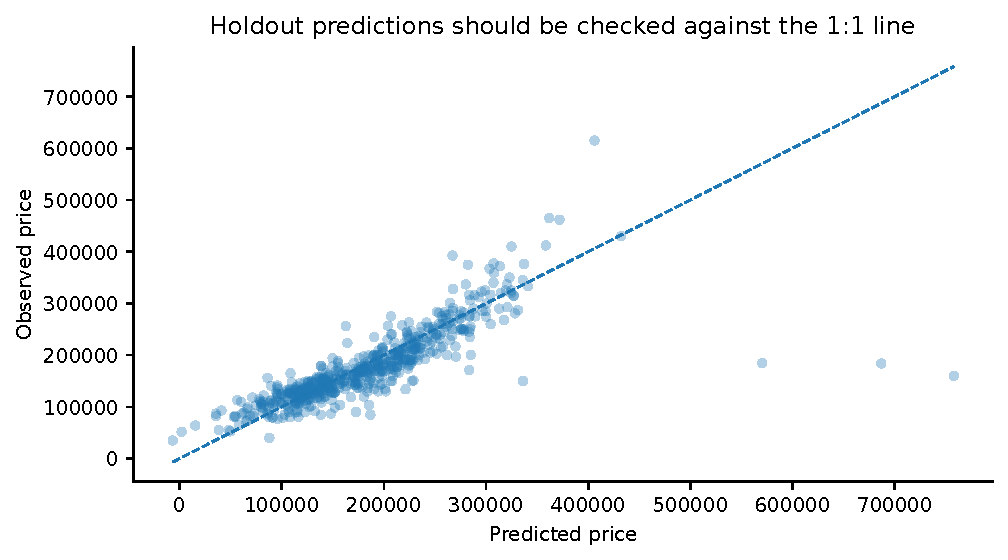
\includegraphics[width=0.66\linewidth]{figures/regression_predicted_actual.pdf}
\end{utpfig}

\section{Linear-model assumptions are diagnostic questions}
For inference on coefficients, common assumptions include approximate linearity of the conditional mean, independent errors, constant error variance, and an error distribution suitable for the inferential approximation. For prediction, the practical emphasis shifts toward whether residual patterns indicate systematic failure on cases like those to be predicted.

\begin{utpfig}[Residual diagnostic]{A useful residual plot looks roughly patternless around zero. Curvature, funnels, clusters, or isolated points suggest model misspecification or heterogeneous error.}{fig:regression-residual-plot}
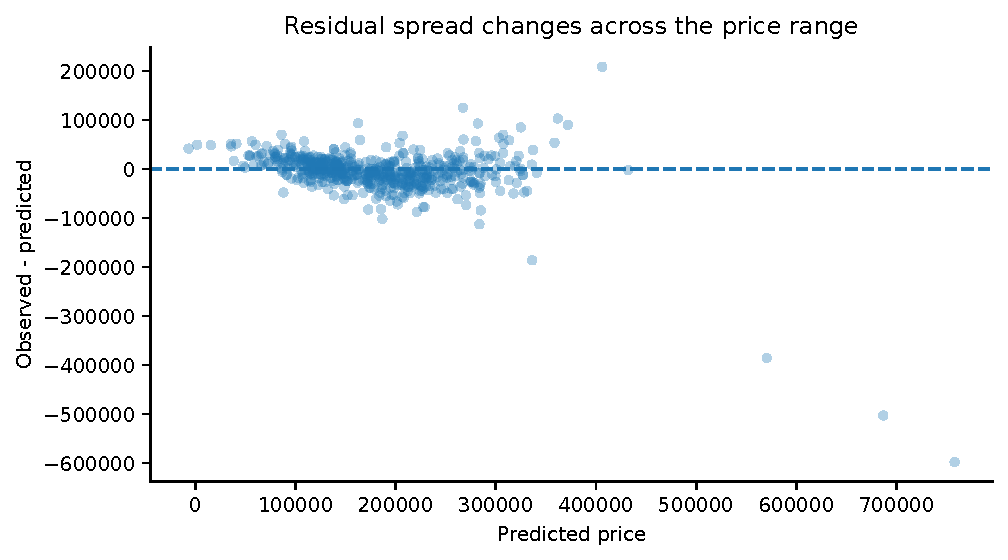
\includegraphics[width=0.79\linewidth]{figures/regression_residual_plot.pdf}
\end{utpfig}

\section{Residuals reveal model failures}
Residual plots can expose curvature, non-constant variance, influential observations, or systematic subgroup errors. A single average metric can hide all of these.

\begin{pitfall}
Evaluating the model on the same rows used for fitting answers ``How well did the model remember the training data?'' rather than ``How well might it generalise?''
\end{pitfall}


\section{Underfitting and overfitting are both prediction problems}
A model that is too rigid can miss genuine structure; a model that is too flexible can fit sample-specific noise. Training error usually decreases with complexity, so model selection must rely on held-out or cross-validated performance.

\begin{utpfig}[Conceptual model-complexity curve]{Training error can keep improving while validation error eventually worsens. The useful level of complexity is determined by generalisation, not by the lowest training error.}{fig:regression-complexity}
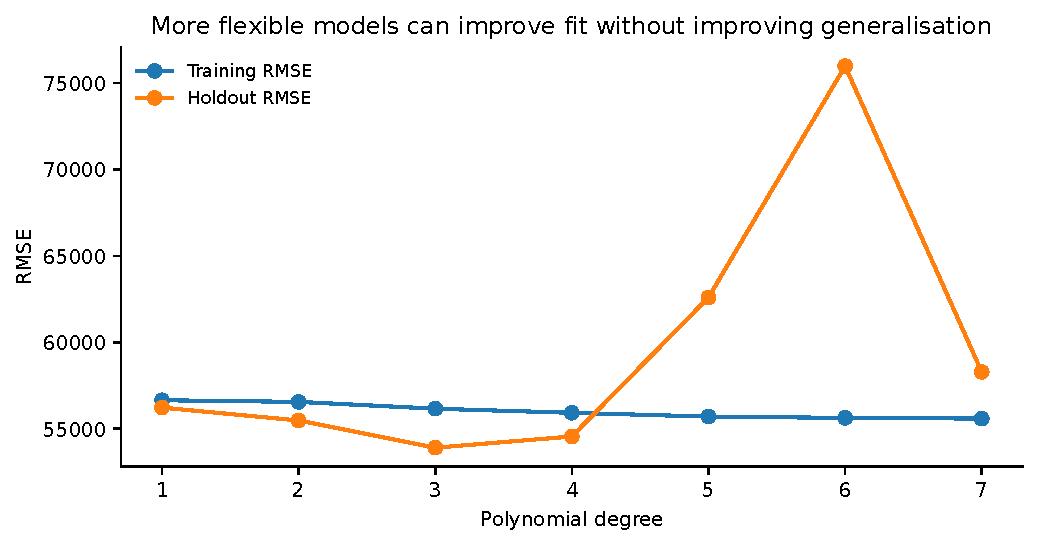
\includegraphics[width=0.80\linewidth]{figures/regression_complexity.pdf}
\end{utpfig}


\section{Baselines make metrics meaningful}
Compare the regression against a simple baseline such as predicting the training-set mean for every case. A model that cannot improve on a naive baseline is not useful merely because it produced coefficients.

\begin{workedexample}
In Lab 7, alcohol is predicted from several other chemical measurements. The point is not to claim a production-ready chemistry model; it is to practise the complete supervised workflow: define target and features, split, fit, predict, evaluate, and inspect residuals.
\end{workedexample}

\begin{keyidea}
A predictive model is an empirical claim about unseen cases. Its credibility comes from validation data and transparent error analysis, not from how impressive the training summary looks.
\end{keyidea}

\begin{quickcheck}
\begin{enumerate}
  \item Why can a low training error be misleading?
  \item How do MAE and RMSE differ in their treatment of large errors?
  \item What can residuals reveal that \(R^2\) cannot?
  \item Why is a simple baseline useful?
\end{enumerate}
\end{quickcheck}

\section{Worked regression context: Ames Housing}

Ames Housing is deliberately more realistic than a small textbook regression table: 2,930 properties, 82 columns, mixed variable types, and substantial missingness in some attributes. The median sale price is \$160,000. Two strong raw associations are \texttt{Overall Qual} with sale price (correlation about 0.80) and above-ground living area with sale price (about 0.71).

\begin{utpfig}[Size, quality, and sale price]{Living area is positively related to sale price, but colour by overall quality reveals that similarly sized homes can occupy very different price ranges. Multivariable regression is useful precisely because one predictor rarely carries the whole structure.}{fig:reg-ames-area}
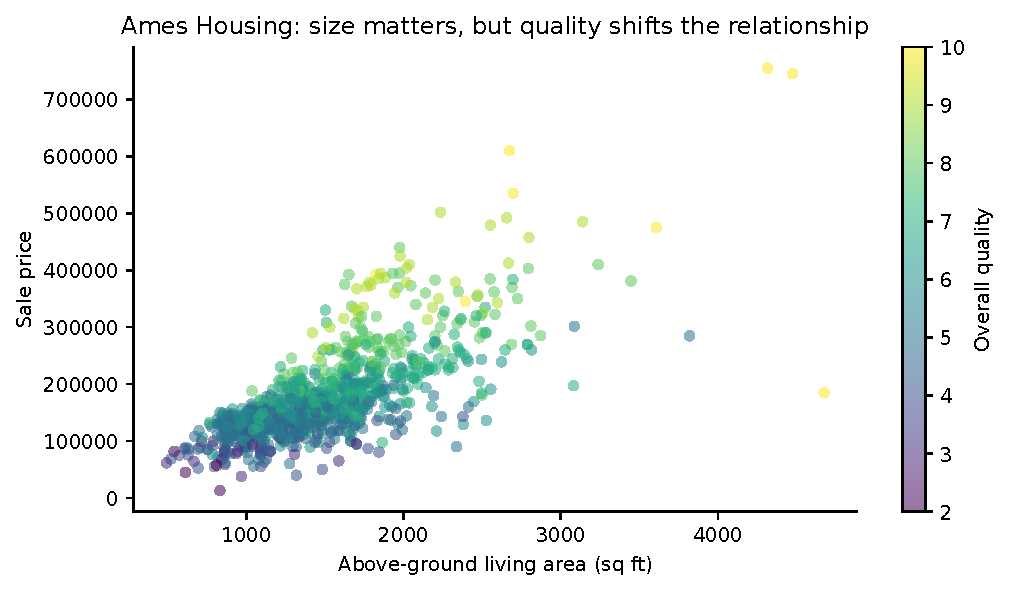
\includegraphics[width=0.86\linewidth]{figures/regression_ames_area_price.pdf}
\end{utpfig}

A model can report a respectable $R^2$ and still fail in patterned ways. Diagnostic plots are therefore part of the model, not optional decoration.

\begin{utpfig}[Residual structure in a simple Ames model]{Residuals are observed minus fitted sale price. Curvature, changing spread, or extreme vertical deviations indicate information not captured by a simple linear specification.}{fig:reg-ames-residuals}
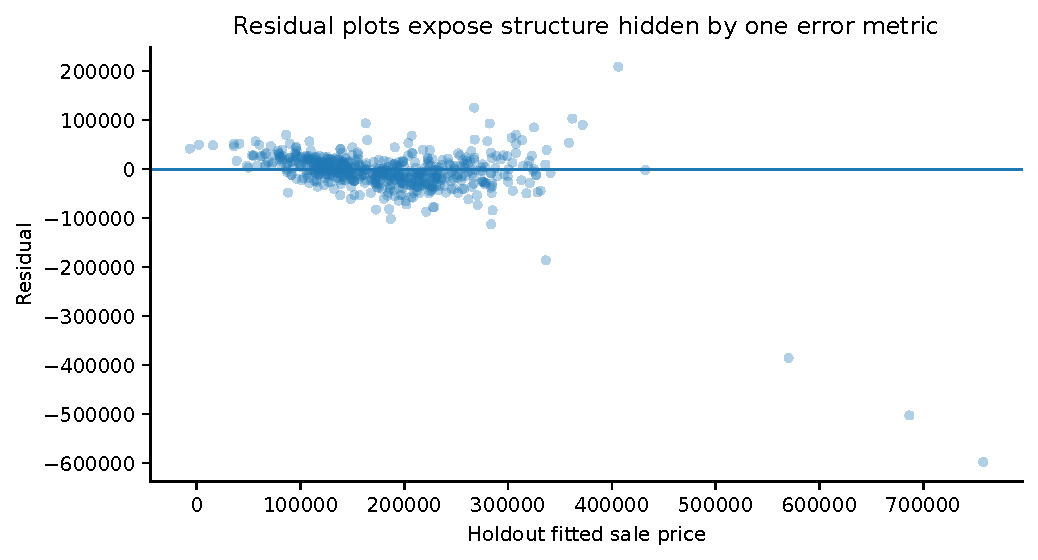
\includegraphics[width=0.82\linewidth]{figures/regression_ames_residuals.pdf}
\end{utpfig}

Ames also introduces an important modelling decision: many categorical variables such as neighbourhood, building type, and exterior quality may be predictive, but including them requires careful encoding and stronger validation. The Lab 7 model starts with a small interpretable subset so students can diagnose the workflow before increasing complexity.


\section{Categorical predictors can carry structure that numeric summaries miss}

Ames Housing contains many categorical variables whose levels represent location, construction, or condition. Neighbourhood is a useful example because it produces clear price differences while also raising modelling questions about sparse levels, interpretation, and generalisation to future properties.

\begin{utpfig}[Neighbourhood groups have different price distributions]{The figure shows median sale price for neighbourhoods with at least 40 observations. The labels report group size so that a large median difference is not interpreted without knowing how much evidence supports it.}{fig:reg-ames-neighborhood}
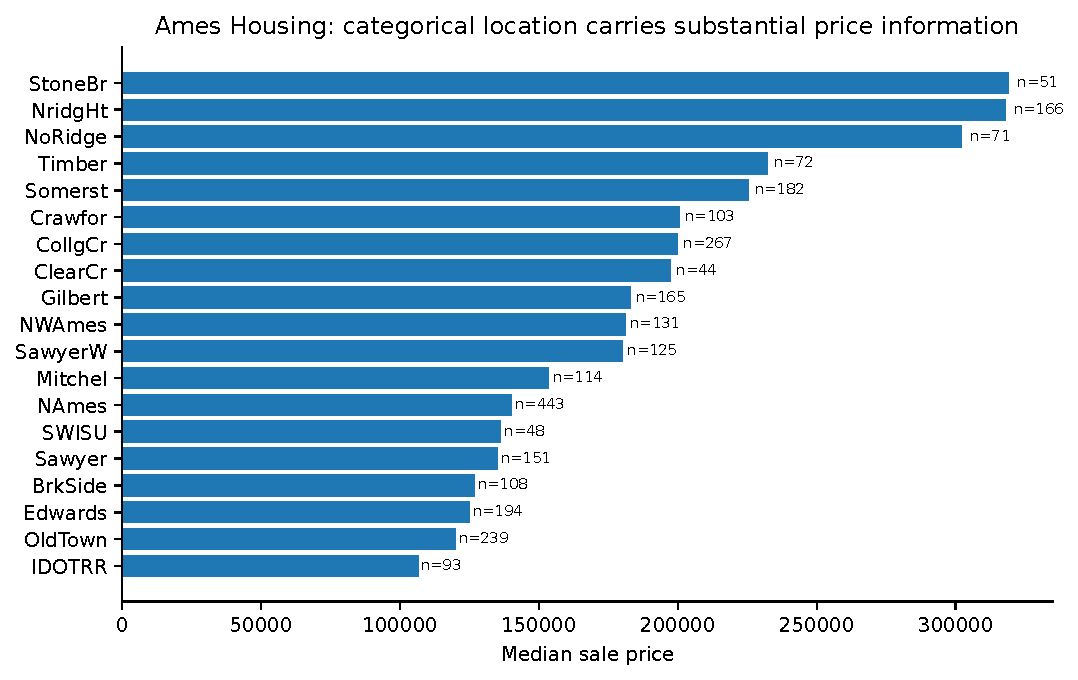
\includegraphics[width=0.88\linewidth]{figures/regression_ames_neighborhood.pdf}
\end{utpfig}

A regression model cannot consume neighbourhood names as unordered text. Common approaches create indicator variables, combine rare levels, or use regularised encodings learned only from the training set. Whatever representation is chosen becomes part of the preprocessing pipeline and must therefore be reproduced exactly at prediction time.

\begin{pitfall}
Encoding a category using the target mean calculated from the full dataset is leakage. If target encoding is used, the encoding itself must be learned inside the training fold and applied to the corresponding validation fold without using its outcomes.
\end{pitfall}

\labsection{7}{Build and diagnose a regression model}{sec:lab07}

\begin{labproject}{Regression: predict, benchmark, and diagnose}
\textbf{Coverage.} Chapter~\ref{ch:regression}.\\
\textbf{Goal.} You should be able to construct a leakage-safe train/test workflow, compare a model with a baseline, interpret holdout metrics, inspect residual structure, and evaluate whether a categorical predictor adds useful generalisable information.\\
\textbf{Dataset.} \texttt{ames\_housing\_dataset.csv}.\\
\textbf{Scenario.} You are building a first house-price prediction model. The goal is not to maximise fit on the available data, but to establish a transparent baseline, estimate performance on unseen records, and identify where the model fails.

\textbf{Core workflow.}
\begin{enumerate}
  \item \textbf{Define target and predictors.} Use \texttt{SalePrice} as the target and begin with living area, overall quality, year built, garage capacity, and basement area. Explain why each predictor is available before the sale outcome.
  \item \textbf{Handle missingness transparently.} Report the original row count, the rows removed or modified for selected variables, and the final modelling sample.
  \item \textbf{Split before fitting.} Create a reproducible 80/20 train/test split. Keep the test set untouched until model evaluation.
  \item \textbf{Establish a baseline.} Predict the training-set median sale price for every test record. Compute baseline MAE and RMSE before evaluating the regression model.
  \item \textbf{Fit multiple regression.} Fit the specified linear model on training data only. Interpret coefficient signs conditionally and avoid causal language.
  \item \textbf{Evaluate generalisation.} On the test set, report MAE, RMSE, and $R^2$, then quantify improvement over the baseline.
  \item \textbf{Diagnose failure modes.} Inspect predicted-versus-observed and residual-versus-fitted plots. Identify nonlinearity, changing variance, systematic under/overprediction, or influential extreme errors.
  \item \textbf{Inspect segment error.} Compare absolute error across sale-price bands or another meaningful subgroup. Determine whether a good average metric hides poor performance for a subset of homes.
\end{enumerate}

\textbf{Model-development extension.} Examine neighbourhood sample sizes and median prices before adding \texttt{Neighborhood} as a categorical predictor. Refit using the same split and report whether holdout error improves. Explain why any target-derived encoding must be learned from training data only.

\tcbbreak
\lstinputlisting[style=utpr]{all_experiments/lab07_regression.R}
\begin{verification}
\textbf{Required evidence.} Submit baseline and model metrics, two diagnostic plots, one subgroup error summary, and a short model card stating intended use, strongest observed limitation, and one next improvement to test.

\textbf{Professional standard.} A model is useful only relative to a baseline and an intended decision. Training $R^2$ alone is not evidence of predictive performance.
\end{verification}
\end{labproject}


\chapter{Classification and Decision Thresholds}
\label{ch:classification}
\chapterguide
  {You should understand train/test evaluation and numeric prediction metrics.}
  {fit a binary logistic model, convert probabilities to decisions, construct a confusion matrix, and explain accuracy, precision, sensitivity, and specificity.}

\section{Classification predicts categories}
A binary classifier estimates evidence for one of two outcomes, such as fraud/not fraud, churn/stay, or malignant/benign. Many classifiers first produce a probability-like score and then apply a threshold to make a class decision.

For logistic regression,
\[
P(Y=1\mid x)=\frac{1}{1+e^{-\eta}},
\qquad
\eta=\beta_0+\beta_1x_1+\cdots+\beta_px_p.
\]


\section{Logistic regression models log-odds linearly}
The logistic curve converts the unconstrained linear predictor $\eta$ into a value between zero and one. Equivalently,
\[
\log\left(\frac{p}{1-p}\right)=\beta_0+\beta_1x_1+\cdots+\beta_px_p,
\]
so each coefficient changes the \term{log-odds} of the positive class conditionally on the other included variables. Exponentiating a coefficient gives an odds ratio for a one-unit feature change, but this remains an associational model unless the design supports causal interpretation.

\begin{utpfig}[Logistic transformation]{The S-shaped logistic function compresses extreme linear scores toward probabilities near 0 and 1 while mapping a score of zero to probability 0.5.}{fig:classification-sigmoid}
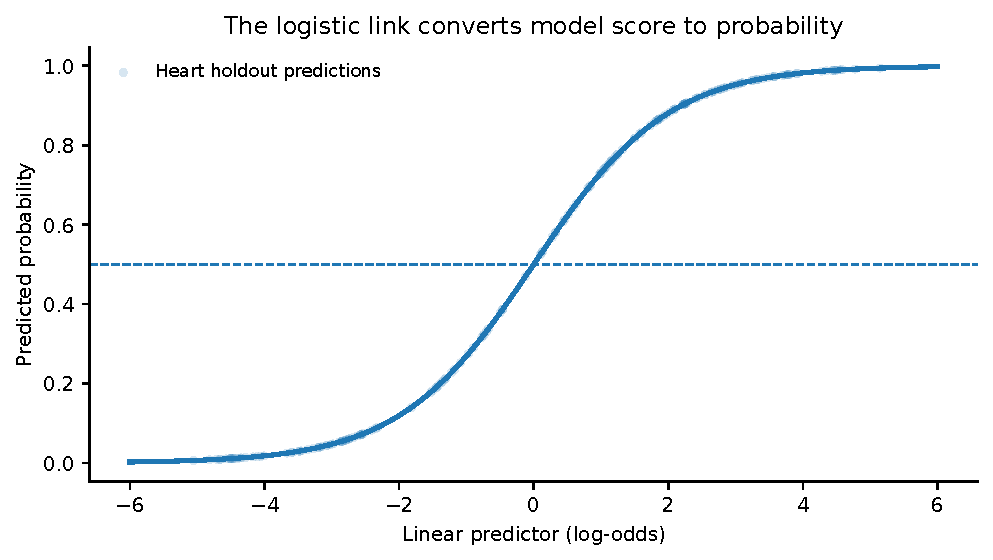
\includegraphics[width=0.80\linewidth]{figures/classification_sigmoid.pdf}
\end{utpfig}

\section{The confusion matrix is the evaluation foundation}
\begin{utptable}
\begin{tabularx}{\linewidth}{@{}>{\bfseries\leavevmode\color{UTPNavy}}m{2.8cm}YD{5.5cm}@{}}
\toprule
\rowcolor{UTPPaleBlue!92}
\utpth{Outcome} & \utpth{Meaning} & \utpth{Example in a medical screening context} \\
\midrule
True positive & predicted positive, actually positive & malignant case flagged \\
False positive & predicted positive, actually negative & benign case flagged \\
True negative & predicted negative, actually negative & benign case not flagged \\
False negative & predicted negative, actually positive & malignant case missed \\
\bottomrule
\end{tabularx}
\end{utptable}

From these counts:
\[
\text{Sensitivity}=\frac{TP}{TP+FN},\qquad
\text{Specificity}=\frac{TN}{TN+FP},\qquad
\text{Precision}=\frac{TP}{TP+FP}.
\]
Accuracy is \((TP+TN)/N\).


\begin{utpfig}[Confusion matrix from a held-out teaching split]{Counts retain the direction of each mistake. Reporting only accuracy would hide whether errors are mostly false positives or false negatives.}{fig:classification-cm}
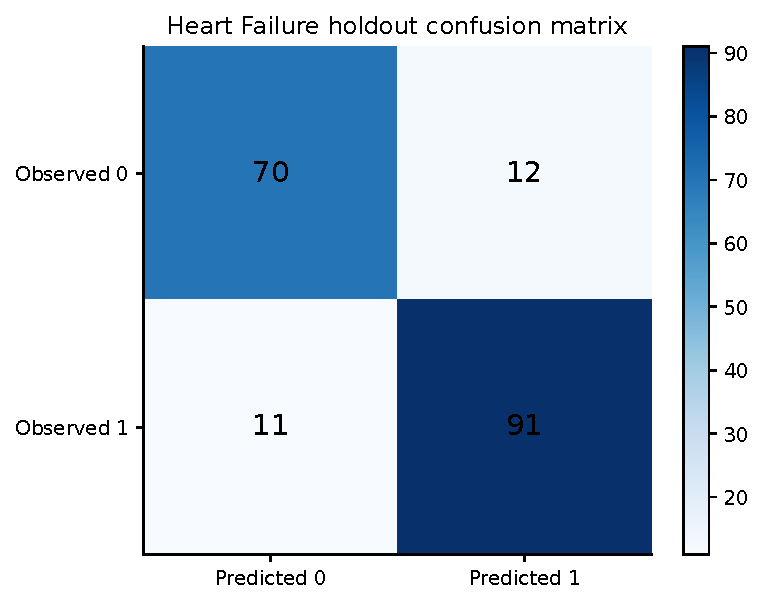
\includegraphics[width=0.58\linewidth]{figures/classification_confusion_matrix.pdf}
\end{utpfig}

\section{Metrics answer different operational questions}
Sensitivity asks, ``Of the actual positives, how many did we find?'' Specificity asks the corresponding question for negatives. Precision asks, ``Of the cases we flagged positive, how many were actually positive?'' These denominators differ, so the metrics answer different questions.

Precision is especially sensitive to prevalence. A classifier can have similar sensitivity and specificity in two populations but very different precision if the event is much rarer in one population.


\section{Accuracy can fail on imbalanced data}
If 99\% of cases are negative, predicting ``negative'' every time yields 99\% accuracy and zero ability to find positives. Metric choice must reflect the operational cost of mistakes.

\begin{pitfall}
There is no universally correct threshold of 0.5. Lowering the threshold usually catches more positives but also creates more false positives. The right trade-off depends on consequences, prevalence, and downstream capacity.
\end{pitfall}


\begin{utpfig}[Where classification errors come from]{Predicted-score distributions for the two classes overlap. Moving the threshold changes which part of the overlap becomes false positive or false negative.}{fig:classification-overlap}
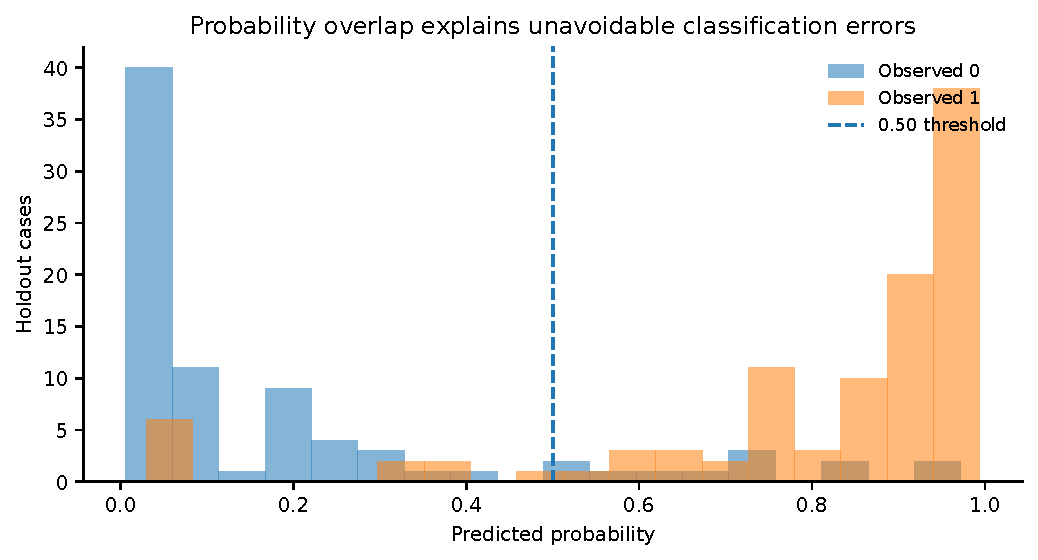
\includegraphics[width=0.82\linewidth]{figures/classification_score_overlap.pdf}
\end{utpfig}


\begin{utpfig}[Threshold trade-off]{The probability model and the decision rule are separate. Changing the threshold can change false-negative and false-positive rates without refitting the model.}{fig:threshold-tradeoff}
\begin{tikzpicture}[x=\linewidth,y=1cm,
  stage/.style={draw=UTPBlue!65,fill=UTPPaleBlue,rounded corners=1.8mm,
    line width=0.7pt,text width=0.14\linewidth,
    minimum width=0.19\linewidth,minimum height=1.70cm,
    inner xsep=3mm,inner ysep=2.5mm,align=center,
    font=\scriptsize\color{UTPNavy}},
  flow/.style={-{Stealth[length=2.2mm,width=1.6mm]},
    line width=0.9pt,draw=UTPTeal}]
\node[stage,draw=UTPTeal!80,fill=UTPPaleTeal] (p) at (0.11,0)
  {\textcolor{UTPTeal}{\textbf{01  SCORE}}\\[5pt]
   \textbf{Model outputs}\\[4pt]
   Scores or probabilities};
\node[stage,draw=UTPOrange!80,fill=UTPPaleOrange] (t) at (0.37,0)
  {\textcolor{UTPOrange!85!black}{\textbf{02  THRESHOLD}}\\[5pt]
   \textbf{Choose cutoff}\\[4pt]
   Set the decision rule};
\node[stage] (d) at (0.63,0)
  {\textcolor{UTPBlue}{\textbf{03  DECIDE}}\\[5pt]
   \textbf{Class decisions}\\[4pt]
   Positive or negative};
\node[stage,draw=UTPTeal!80,fill=UTPPaleTeal] (c) at (0.89,0)
  {\textcolor{UTPTeal}{\textbf{04  EVALUATE}}\\[5pt]
   \textbf{Measure errors}\\[4pt]
   Confusion matrix and costs};
\draw[flow] (p.east) -- (t.west);
\draw[flow] (t.east) -- (d.west);
\draw[flow] (d.east) -- (c.west);
\end{tikzpicture}
\end{utpfig}


\begin{utpfig}[Metrics change with the threshold]{Sensitivity, specificity, and precision move differently as the same fitted model is evaluated at different decision thresholds. The choice must be connected to real error costs.}{fig:classification-threshold-metrics}
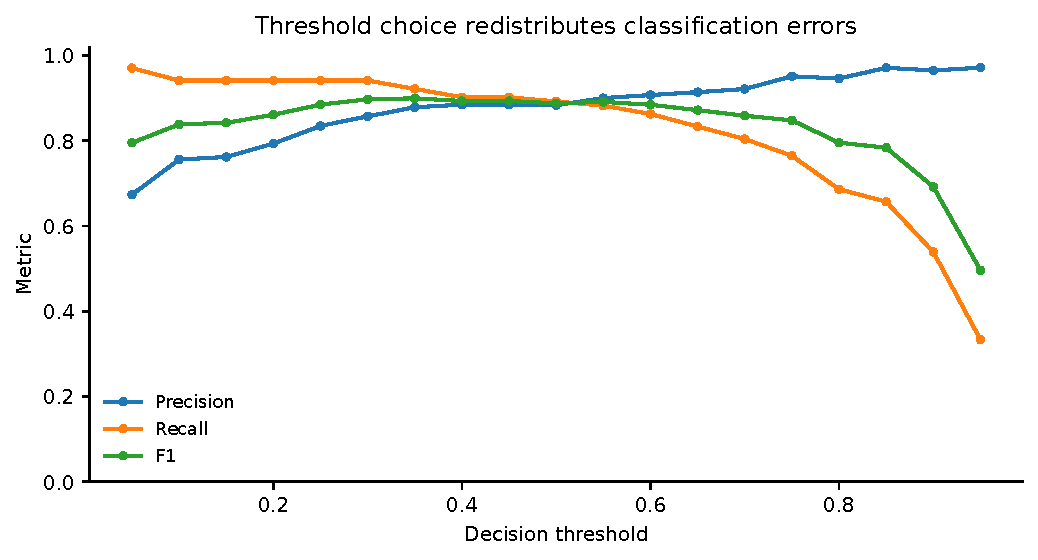
\includegraphics[width=0.84\linewidth]{figures/classification_threshold_metrics.pdf}
\end{utpfig}

\section{Ranking, discrimination, and calibration are different}
A model can rank positive cases above negative cases well but still produce poorly calibrated probabilities. Conversely, a model can be reasonably calibrated overall yet weak at separating individual cases. Receiver-operating-characteristic and precision--recall curves summarise threshold behaviour across many cutoffs, while calibration plots compare predicted probabilities with observed event frequencies.

No single curve removes the need to choose an operating point when the system must ultimately make decisions.


\section{Probabilities need interpretation, not just labels}
A probability output lets analysts rank cases and choose thresholds. It should still be checked for calibration: among cases assigned around 0.8 risk, does the event occur roughly 80\% of the time? Calibration is distinct from classification accuracy.

\begin{workedexample}
In Lab 8 the target is \texttt{HeartDisease} in the bundled heart-failure dataset. The exercise demonstrates probability estimation and error metrics. It is not a clinical diagnostic system and should not be interpreted as one.
\end{workedexample}

\begin{keyidea}
Classification performance is multi-dimensional. Always ask which error matters, for whom, and under what prevalence and deployment conditions.
\end{keyidea}

\begin{quickcheck}
\begin{enumerate}
  \item Why can accuracy be misleading with rare positive cases?
  \item What does sensitivity measure?
  \item What happens to false positives and false negatives when a threshold changes?
  \item Why is calibration different from accuracy?
\end{enumerate}
\end{quickcheck}

\section{Two classification datasets, two different lessons}

The Heart Failure and Breast Cancer datasets both have binary outcomes, but they illustrate different modelling issues.

\begin{utpfig}[Heart-disease classes overlap in ordinary measurements]{Age and maximum heart rate provide useful signal but no clean separating boundary. Logistic regression therefore estimates a probability rather than claiming that one measurement combination deterministically defines disease.}{fig:class-heart}
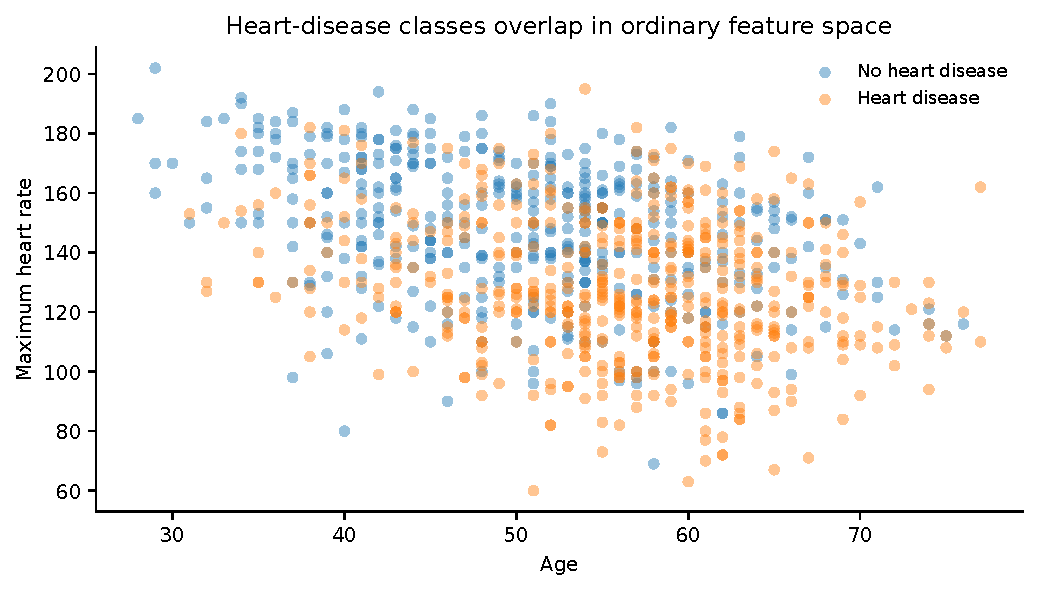
\includegraphics[width=0.80\linewidth]{figures/classification_heart_age_maxhr.pdf}
\end{utpfig}

Heart disease is present in about 55.3\% of the 918 records. Mean maximum heart rate is lower in the labelled heart-disease group (about 128) than in the non-disease group (about 148), but the distributions overlap. Categorical predictors such as chest-pain type and ST slope contribute information that cannot be represented by this two-dimensional picture.

\begin{utpfig}[Breast-cancer measurements show partial separation]{Mean radius and mean texture separate many benign and malignant records, yet overlap remains. The full dataset includes many related measurements, creating both predictive opportunity and redundancy.}{fig:class-breast}
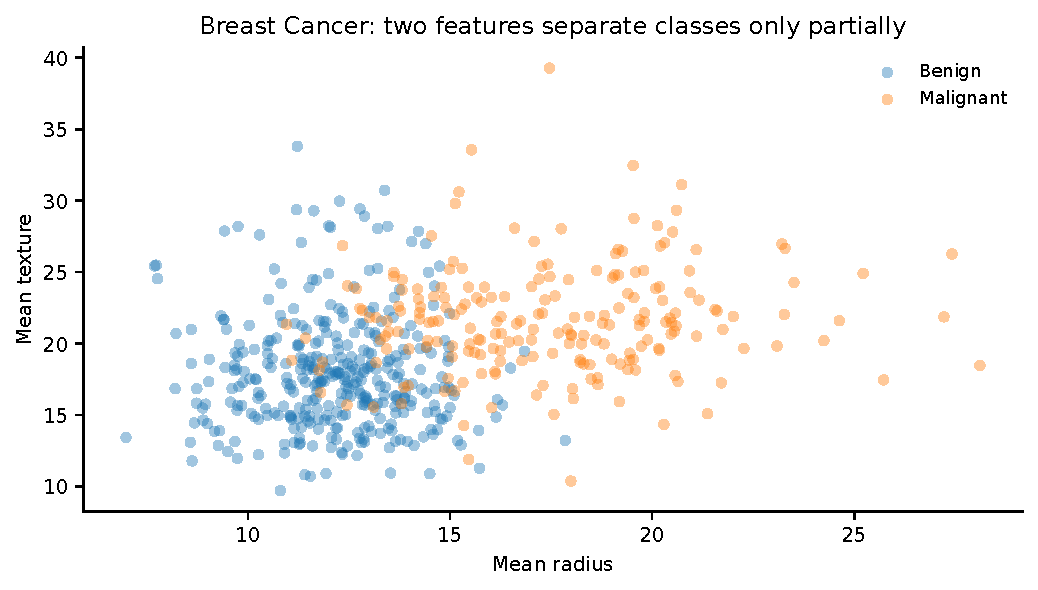
\includegraphics[width=0.80\linewidth]{figures/classification_breast_features.pdf}
\end{utpfig}

In the Breast Cancer file, about 37.3\% of records are malignant. Mean radius averages about 17.46 for malignant records versus 12.15 for benign records. A classifier can exploit such differences, but evaluation must be performed on unseen data and should report error types that match the decision context.

\section{High-dimensional extension: handwritten digits}

The bundled \texttt{optical\_recognition\_handwritten\_digits.zip} contains a training file with 3,823 examples and a test file with 1,797 examples. Each observation contains 64 pixel-intensity features arranged conceptually as an $8\times8$ image plus a digit label from 0 to 9. The values range from 0 to 16 and describe local pixel density rather than a photograph stored as an image file.

\begin{utpfig}[A table row can still represent an image]{The ten panels reconstruct one example of each digit from the 64 numeric feature values. The classifier receives a vector of numbers; the image layout is domain knowledge that helps humans understand what those numbers mean.}{fig:class-digits-examples}
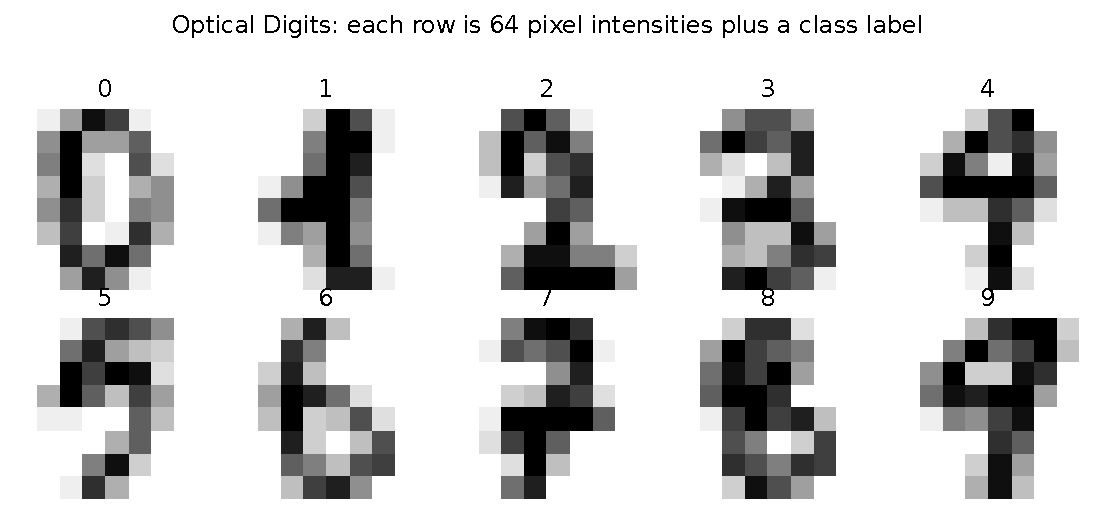
\includegraphics[width=0.86\linewidth]{figures/classification_digits_examples.pdf}
\end{utpfig}

This dataset extends binary classification in three important ways. First, the outcome has ten classes, so evaluation needs a $10\times10$ confusion matrix or per-class metrics rather than one sensitivity/specificity pair. Second, 64 dimensions make direct visualisation impossible. Third, the supplied train/test split reflects different writers, which can be more demanding than randomly mixing records from the same writer across both sets.

\begin{utpfig}[Two dimensions cannot preserve all multiclass structure]{PCA compresses the 64 standardised pixel features into two directions for visual inspection. Some digits form visible regions, but extensive overlap remains; a two-dimensional plot is an interpretation tool, not the classifier itself.}{fig:class-digits-pca}
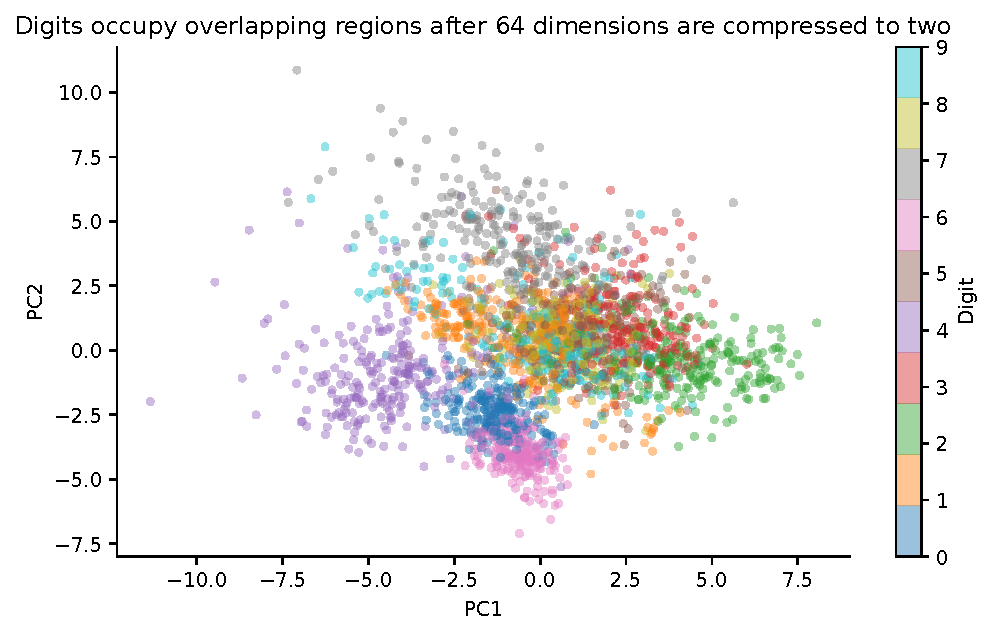
\includegraphics[width=0.80\linewidth]{figures/classification_digits_pca.pdf}
\end{utpfig}

Multiclass performance should be reported at more than one level. Overall accuracy answers ``how often is the label correct?'' while a confusion matrix reveals which digits are confused. Macro-averaged metrics give each digit equal weight; frequency-weighted metrics emphasise common digits. These choices matter whenever class frequencies differ.

\begin{keyidea}
High dimensionality is not only ``many columns.'' It changes distance, visualisation, model complexity, and validation. The digits data provide a bridge from classification to PCA and representation learning while also showing why the data-generating split matters.
\end{keyidea}

\labsection{8}{Evaluate probabilistic classification}{sec:lab08}

\begin{labproject}{Classification: preserve probabilities and make error trade-offs explicit}
\textbf{Coverage.} Chapter~\ref{ch:classification}.\\
\textbf{Goal.} You should be able to create a stratified split, fit logistic regression, evaluate confusion-matrix metrics, compare thresholds, and distinguish binary from multiclass evaluation.\\
\textbf{Datasets.} \texttt{heart\_failure\_dataset.csv}; Breast Cancer and Optical Digits are used as extensions.\\
\textbf{Scenario.} You are evaluating a binary risk classifier. The purpose is to understand probabilistic output, threshold-dependent decisions, and asymmetric errors---not to treat a statistical exercise as a clinical diagnostic system.

\textbf{Core workflow.}
\begin{enumerate}
  \item \textbf{Define the target and prevalence.} Identify the positive class, report its prevalence, and explain why class balance matters for interpretation of accuracy.
  \item \textbf{Prepare predictors.} Convert categorical variables to factors and document any exclusions. Use a stratified 80/20 split so class prevalence is comparable across train and test sets.
  \item \textbf{Fit a probabilistic model.} Train logistic regression on the training set and generate probabilities for the held-out records. Do not convert probabilities to labels prematurely.
  \item \textbf{Evaluate a reference threshold.} At 0.50, construct the confusion matrix and report accuracy, sensitivity, specificity, precision, and the number of false positives/false negatives.
  \item \textbf{Change the decision rule.} Evaluate at least one lower threshold and one higher threshold. Describe which error decreases and which error increases.
  \item \textbf{Inspect score overlap.} Plot or summarise predicted-probability distributions for observed classes. Explain why imperfect separation makes threshold choice unavoidable.
  \item \textbf{Write a use-limitation statement.} State what additional validation, clinical governance, and data-quality evidence would be required before any medical deployment.
\end{enumerate}

\begin{tryit}
\textbf{Extension A---second binary geometry.} In the Breast Cancer dataset, compare \texttt{radius\_mean} and \texttt{texture\_mean} by diagnosis. Identify whether these two features alone visually separate the classes and why visual separation is not a substitute for holdout evaluation.

\textbf{Extension B---multiclass data.} Read the supplied Optical Digits training/test files and reconstruct at least one $8\times8$ digit from its 64 pixel features. Explain how a $10\times10$ confusion matrix, per-class recall, and macro-averaged metrics extend the binary framework.
\end{tryit}

\tcbbreak
\lstinputlisting[style=utpr]{all_experiments/lab08_classification.R}
\begin{verification}
\textbf{Required evidence.} Submit one holdout confusion matrix, a threshold comparison, one probability-distribution view, and a short decision note explaining which error would be more costly in a stated hypothetical use case.
\end{verification}
\end{labproject}


\chapter{Model Validation, Preprocessing, and Responsible Evaluation}
\label{ch:validation}
\chapterguide
  {You should be able to fit and evaluate a supervised model on a held-out test set.}
  {explain cross-validation, avoid preprocessing leakage, compare thresholds, recognise overfitting, and report model limitations responsibly.}

\section{One split is one random experiment}
A single train/test split can produce an optimistic or pessimistic estimate depending on which rows happen to land in the test set. \term{Cross-validation} repeats the evaluation across several held-out folds.

\begin{utpfig}[Five-fold cross-validation]{Each fold acts as validation once while the remaining folds train the model. The final performance summary combines the held-out results.}{fig:five-fold}
\begin{tikzpicture}[x=\linewidth,y=1cm,
  foldcell/.style={draw=UTPBlue!70,fill=UTPPaleBlue,rounded corners=1mm,
    line width=0.6pt,text width=0.13\linewidth,minimum height=0.62cm,
    inner xsep=1mm,inner ysep=1mm,align=center,
    font=\scriptsize\color{UTPNavy}},
  heldout/.style={foldcell,draw=UTPTeal!80,fill=UTPPaleTeal,
    font=\scriptsize\bfseries\color{UTPNavy}},
  heading/.style={font=\scriptsize\bfseries\color{UTPNavy},inner sep=0pt}]
\node[heading,anchor=east] at (0.095,0.65) {Run};
\foreach \c in {0,...,4}{
  \pgfmathtruncatemacro{\foldnumber}{\c+1}
  \node[heading] at (0.20+\c*0.16,0.65) {Fold \foldnumber};
}
\foreach \r in {0,...,4}{
  \pgfmathtruncatemacro{\runnumber}{\r+1}
  \node[heading,anchor=east] at (0.095,-\r*0.78) {\runnumber};
  \foreach \c in {0,...,4}{
    \ifnum\r=\c
      \node[heldout] at (0.20+\c*0.16,-\r*0.78) {Validate};
    \else
      \node[foldcell] at (0.20+\c*0.16,-\r*0.78) {Train};
    \fi
  }
}
\node[font=\scriptsize\color{UTPMuted},align=center,
  text width=0.86\linewidth] at (0.50,-3.85)
  {Each run uses four training folds and one held-out validation fold.};
\end{tikzpicture}
\end{utpfig}


\begin{utpfig}[Cross-validation reveals split variation]{Each bar is held-out accuracy from a different fold of the same five-fold procedure. The variation is part of the uncertainty in generalisation performance.}{fig:validation-fold-variation}
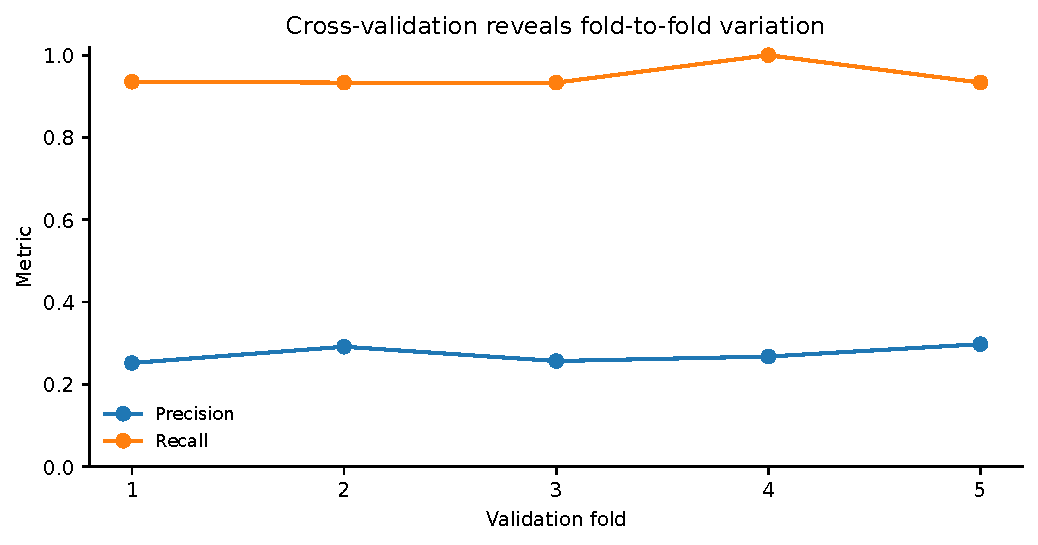
\includegraphics[width=0.79\linewidth]{figures/validation_fold_variation.pdf}
\end{utpfig}

\section{Cross-validation estimates a process, not one final model}
In $k$-fold cross-validation, $k$ temporary models are fitted to estimate how the training procedure generalises. After model choices are fixed, a final model can be refit on all available training data. The fold models are therefore evaluation instruments rather than necessarily the models that will be deployed.

Stratification is useful for classification because it keeps class proportions more consistent across folds. Grouped cross-validation is needed when observations from the same entity must stay together, such as multiple visits from one patient. Time-series data often require forward-chaining splits rather than random folds because future observations must not train models evaluated on the past.


\section{Preprocessing is learned from data}
Centering, scaling, imputation, feature selection, and encoding all estimate information from data. Therefore they belong inside the training process.

Correct order:
\begin{utpsteps}
  \item Split training and validation/test observations.
  \item Estimate preprocessing parameters from training observations only.
  \item Apply those fixed parameters to validation/test observations.
  \item Fit the model on processed training data and evaluate on processed held-out data.
\end{utpsteps}


\begin{utpfig}[Correct versus leaky preprocessing]{Any step that estimates information from data must be fitted inside the training portion of each fold. The validation rows receive parameters learned elsewhere; they do not help create them.}{fig:validation-pipeline}
\begin{tikzpicture}[x=\linewidth,y=1cm,
  card/.style={draw=UTPBlue!70,fill=UTPPaleBlue,rounded corners=1.5mm,
    line width=0.6pt,text width=0.26\linewidth,minimum height=1.45cm,
    inner xsep=2.5mm,inner ysep=2mm,align=center,
    font=\scriptsize\color{UTPNavy}},
  warning/.style={card,draw=UTPRed!80,fill=UTPPaleRed},
  flow/.style={-{Stealth[length=2mm,width=1.5mm]},
    line width=0.8pt,draw=UTPTeal,rounded corners=1.5mm},
  heading/.style={font=\scriptsize\bfseries\color{UTPNavy},anchor=west}]
\node[heading,text=UTPTeal!85!black] at (-0.145,1.1)
  {Correct: learn preprocessing from training rows only};
\node[card] (tr) at (0,0) {\textbf{Training fold}\\[4pt]
  Training observations\\only};
\node[card] (fit) at (0.335,0) {\textbf{Fit preprocessing}\\[4pt]
  Imputer, scaler,\\and feature selector};
\node[card,draw=UTPOrange!80,fill=UTPPaleOrange] (va) at (0.335,-1.8)
  {\textbf{Validation fold}\\[4pt]
   Held-out observations\\Never used for fitting};
\node[card,draw=UTPTeal!80,fill=UTPPaleTeal] (ev) at (0.670,0)
  {\textbf{Transform / evaluate}\\[4pt]
   Apply fixed training rules\\to held-out data};
\draw[flow] (tr.east) -- (fit.west);
\draw[flow] (fit.east) -- (ev.west);
\draw[flow] (va.east) -- (0.670,-1.8) -- (ev.south);
\draw[UTPMuted!35,line width=0.5pt] (-0.145,-2.9) -- (0.815,-2.9);
\node[heading,text=UTPRed!85!black] at (-0.145,-3.3)
  {Leaky: validation rows influence preprocessing};
\node[warning] (all) at (0,-4.4) {\textbf{All observations}\\[4pt]
  Training and validation\\rows combined};
\node[warning] (leakyfit) at (0.335,-4.4) {\textbf{Fit preprocessing}\\[4pt]
  Learn parameters\\from all rows};
\node[warning] (split) at (0.670,-4.4) {\textbf{Split / validate}\\[4pt]
  Held-out information\\has already leaked};
\draw[flow,draw=UTPRed!80] (all.east) -- (leakyfit.west);
\draw[flow,draw=UTPRed!80] (leakyfit.east) -- (split.west);
\end{tikzpicture}
\end{utpfig}

\begin{pitfall}
Scaling the full dataset before cross-validation lets each validation fold influence its own preprocessing. The leakage may be small in some datasets, but the evaluation principle is still broken.
\end{pitfall}

\section{Standardisation aligns feature scales}
For feature \(x\), standardisation uses
\[
z=\frac{x-\mu_{train}}{\sigma_{train}}.
\]
This is important for distance-based and regularised methods. Tree-based models are much less sensitive to monotonic scaling, which is why preprocessing should match the algorithm rather than be applied ritualistically.


\begin{utpfig}[Why scaling changes geometry]{Raw features can have completely different numerical ranges. Standardisation places them in standard-deviation units, which matters when distances or coefficient penalties compare features directly.}{fig:validation-scaling}
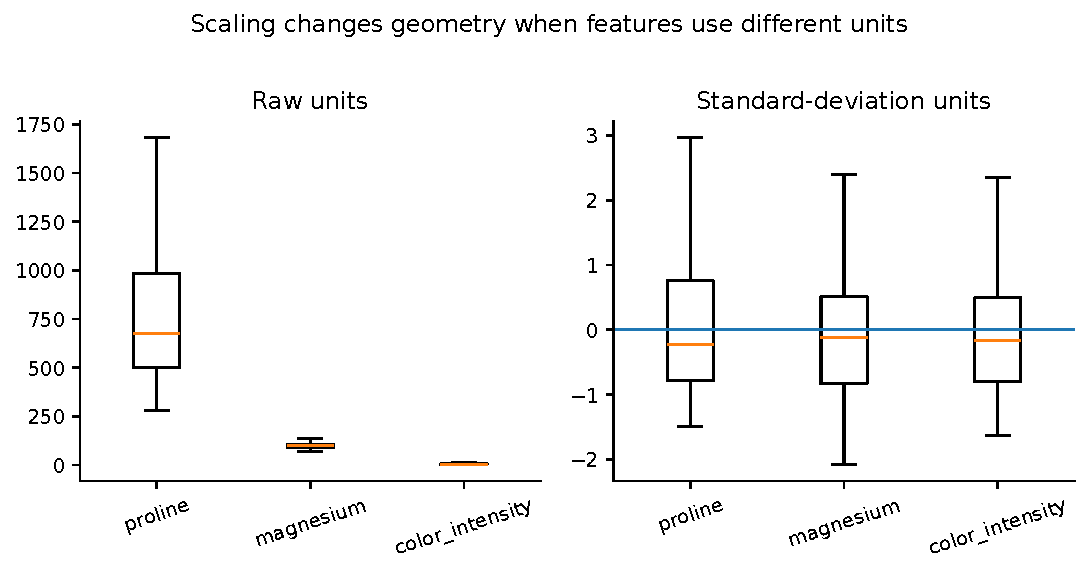
\includegraphics[width=0.92\linewidth]{figures/validation_scaling.pdf}
\end{utpfig}

\begin{utpfig}[Scaling does not make distributions identical]{After standardisation the selected features share center and scale units, but their shapes remain different. Preprocessing changes representation; it does not make the data Gaussian or remove outliers.}{fig:validation-scaled-shapes}
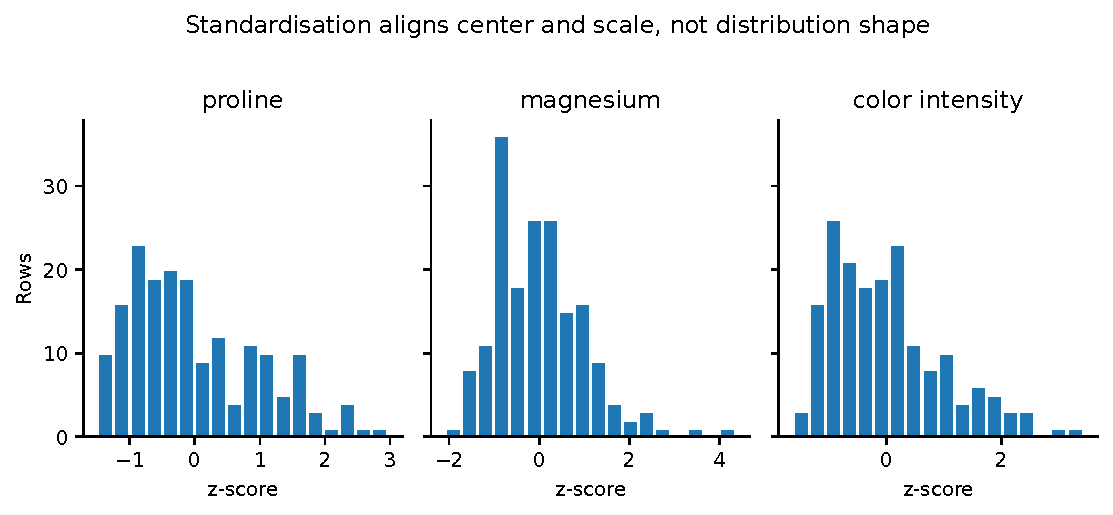
\includegraphics[width=0.80\linewidth]{figures/validation_scaled_distributions.pdf}
\end{utpfig}

\section{Hyperparameter tuning needs its own validation logic}
When cross-validation is used repeatedly to choose model complexity, features, or hyperparameters, the chosen configuration can become optimistic with respect to those same folds. A separate final test set or nested cross-validation provides a cleaner estimate of performance after tuning.

This principle generalises: any choice influenced by evaluation data---including threshold selection, feature selection, and architecture choice---has consumed some information from those data.


\section{Overfitting is a gap between fit and generalisation}
Overfitting occurs when a model captures training-specific noise or idiosyncrasy. Symptoms include excellent training performance with substantially poorer held-out performance and unstable results across folds.

\section{Thresholds, metrics, and stakeholder costs}
Different thresholds produce different confusion matrices. Model evaluation should include the metrics relevant to the actual action: detecting positives, avoiding false alarms, controlling workload, or balancing costs.


\section{Report the distribution of performance, not only the mean}
A mean cross-validation score can hide instability. Report fold scores, their spread, and any unusually weak fold. If performance depends strongly on one split, investigate whether data scarcity, subgroup imbalance, temporal drift, or duplicated entities are responsible.

\section{Subgroup evaluation needs careful denominators}
When performance is compared across groups, show group sample sizes and uncertainty as well as point metrics. A large difference in estimated error rates can be mostly sampling noise when a subgroup is small. Conversely, a good overall score can hide systematic failure in an important subgroup.


\section{Responsible evaluation goes beyond a single metric}
Check performance by meaningful subgroups when appropriate, report data provenance and exclusions, disclose uncertainty, and distinguish a teaching exercise from a deployable system. Protected or sensitive attributes require particularly careful governance and fairness analysis.

\begin{keyidea}
A model report should make failure visible: where the data came from, what preprocessing was learned, how validation was performed, which errors remain, and where the model should not be used.
\end{keyidea}

\begin{workedexample}
Lab 9 estimates scaling parameters separately inside each fold before fitting logistic regression. This small implementation detail is a core scientific principle: held-out data must remain genuinely held out.
\end{workedexample}

\begin{quickcheck}
\begin{enumerate}
  \item What does cross-validation improve compared with one random split?
  \item Which data should determine the scaling mean and standard deviation?
  \item Name one symptom of overfitting.
  \item Why might two stakeholders choose different classification thresholds for the same model?
\end{enumerate}
\end{quickcheck}

\section{Worked validation problem: rare-event fraud detection}

Credit-card fraud is a classic example of why validation metrics must match the data-generating problem. In the bundled 10,000-transaction file, only 151 records are labelled fraud---a prevalence of 1.51\%.

\begin{utpfig}[Rare classes make accuracy deceptive]{A classifier that predicts every transaction as legitimate would already achieve 98.49\% accuracy. The right panel shows that some features nevertheless differ sharply between fraud and legitimate transactions.}{fig:val-fraud-imbalance}
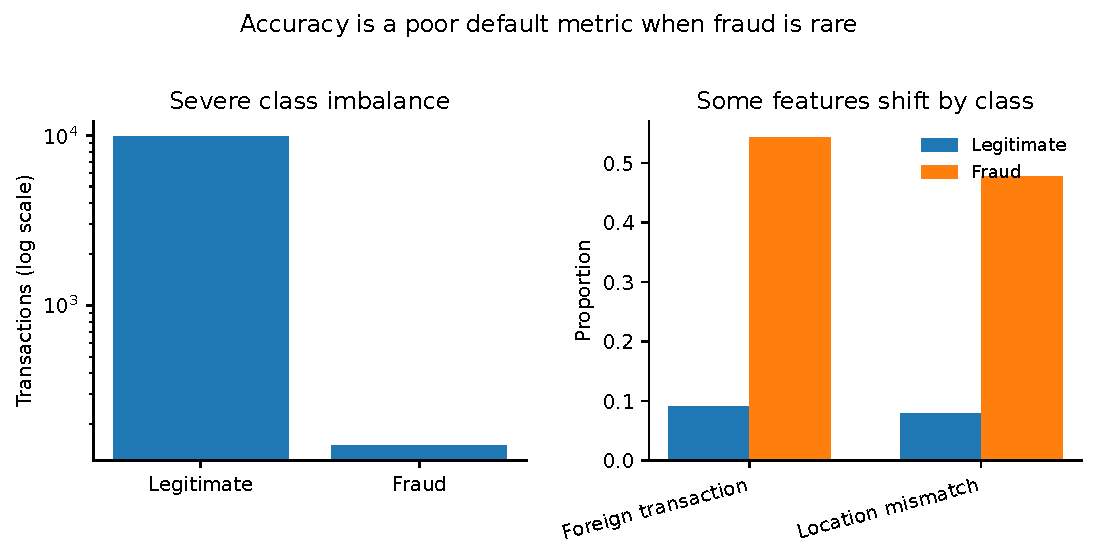
\includegraphics[width=0.90\linewidth]{figures/validation_fraud_imbalance.pdf}
\end{utpfig}

This is why precision, recall/sensitivity, specificity, false-positive rate, and threshold choice must be considered together. The best operating point depends on the relative cost of interrupting a legitimate customer versus missing a fraudulent transaction.

\begin{utpfig}[A threshold converts probabilities into operational decisions]{Changing the decision threshold moves the model along a precision--recall trade-off. Validation should compare thresholds on held-out data rather than selecting a threshold from training performance.}{fig:val-fraud-threshold}
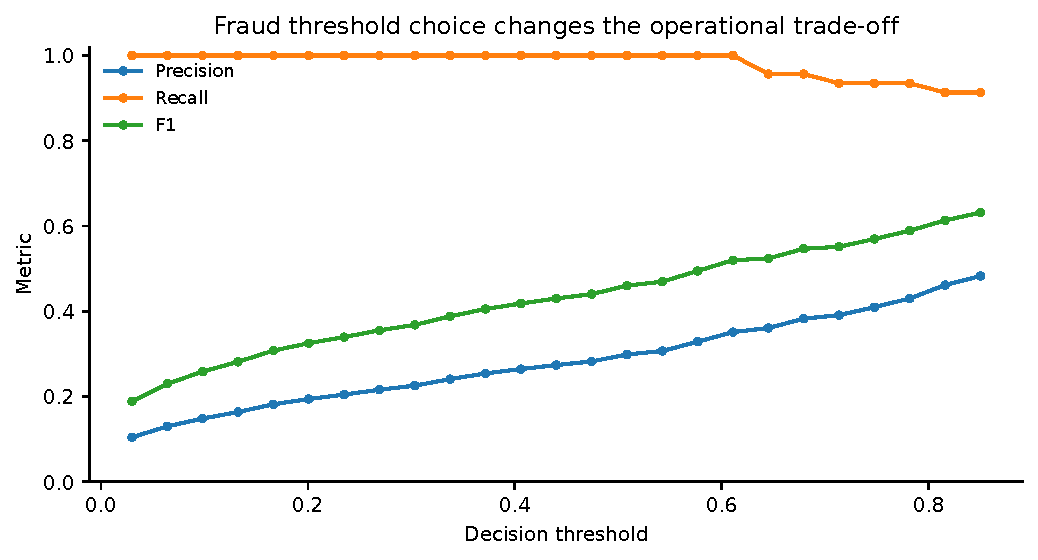
\includegraphics[width=0.82\linewidth]{figures/validation_fraud_thresholds.pdf}
\end{utpfig}

Fraud examples also make preprocessing leakage easier to understand. If scaling parameters, category encodings, resampling rules, or threshold choices are tuned using the full dataset before cross-validation, information from validation folds has influenced the training pipeline even if the final model never directly sees their labels.


\section{Calibration is a validation target when probabilities drive action}

A classifier can rank cases well while producing probabilities that are systematically too high or too low. This distinction matters when a probability is used for triage, pricing, resource allocation, or threshold selection. Calibration compares predicted probability with observed event frequency among cases receiving similar scores.

\begin{utpfig}[Heart-disease probability calibration on held-out data]{Points near the diagonal indicate agreement between predicted probability and observed positive frequency within score bins. Departures from the diagonal are a reason to investigate calibration, sample size, model specification, or distribution shift.}{fig:validation-heart-calibration}
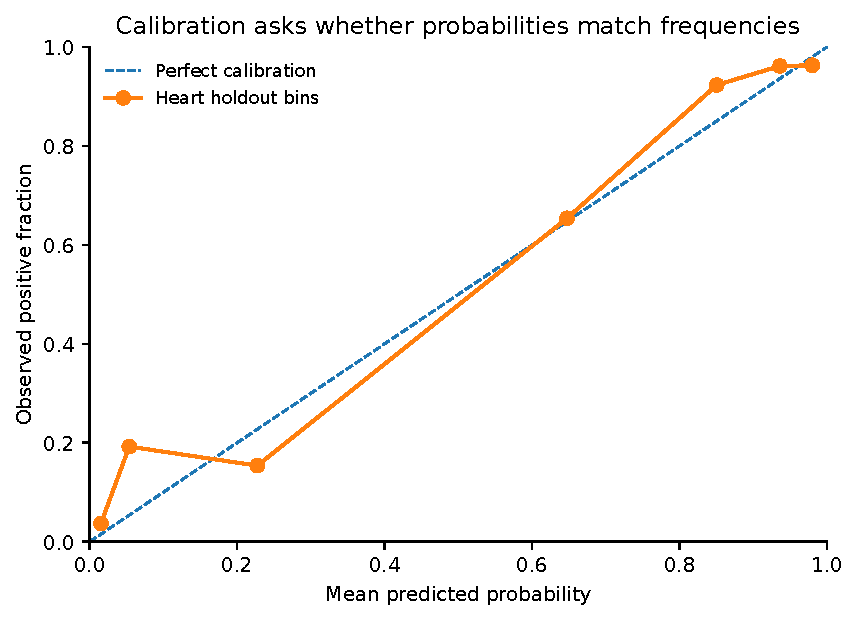
\includegraphics[width=0.68\linewidth]{figures/validation_heart_calibration.pdf}
\end{utpfig}

Calibration should be estimated on data that did not fit the model. If a separate calibration method is learned, it needs its own validation discipline as well. A well-calibrated probability is still not a causal probability, and good calibration in one population does not guarantee calibration after deployment conditions change.

\labsection{9}{Validate an imbalanced classifier without leakage}{sec:lab09}

\begin{labproject}{Validation and preprocessing: evaluate the process, not one lucky split}
\textbf{Coverage.} Chapter~\ref{ch:validation}.\\
\textbf{Goal.} You should be able to construct stratified folds, prevent preprocessing leakage, compare thresholds across folds, quantify metric variability, and distinguish discrimination from calibration.\\
\textbf{Datasets.} \texttt{credit\_card\_fraud\_dataset.csv}; Heart Failure is used for a calibration extension.\\
\textbf{Scenario.} Fraud is rare, so a superficially high accuracy can be operationally useless. You must evaluate a complete modelling process with stratified cross-validation, fold-local preprocessing, and threshold-sensitive metrics.

\textbf{Core workflow.}
\begin{enumerate}
  \item \textbf{Measure the class imbalance.} Report fraud prevalence and the accuracy of an ``always legitimate'' classifier. Treat this as the minimum baseline any useful model must beat.
  \item \textbf{Create stratified folds.} Build five folds that each contain fraud and legitimate transactions. Report the class count in every fold.
  \item \textbf{Keep preprocessing inside the fold.} For each validation fold, estimate scaling parameters from the corresponding training folds only, then apply those parameters to validation data.
  \item \textbf{Fit and retain probabilities.} Train logistic regression inside each fold and store validation probabilities so the same predictions can be evaluated at multiple thresholds.
  \item \textbf{Evaluate decision thresholds.} Compare 0.10, 0.25, and 0.50 using accuracy, precision, recall, and specificity. Include false-positive and false-negative counts where useful.
  \item \textbf{Report variability.} Summarise both the mean and fold-to-fold spread of the metrics. Identify whether recall is stable enough to support a reliable operational claim.
  \item \textbf{Choose a threshold from a stated cost.} Define a hypothetical relative cost for missed fraud versus false alarms, then select the threshold that best reflects that priority. Make clear that the cost assumption is external to the model.
\end{enumerate}

\textbf{Calibration extension.} Reuse the Heart Failure modelling workflow, bin held-out predicted probabilities, and compare mean predicted probability with observed event rate. Explain why a model can rank cases well yet still produce poorly calibrated probabilities.

\tcbbreak
\lstinputlisting[style=utpr]{all_experiments/lab09_validation.R}
\begin{verification}
\textbf{Required evidence.} Submit the majority-class baseline, five-fold metric summary, one variability result, and a threshold recommendation tied to an explicit error-cost assumption. Include one sentence identifying where leakage would occur if global scaling were applied before cross-validation.

\textbf{Professional standard.} Validation must reproduce the full future prediction process. Any transformation learned from all records before validation contaminates the estimate of generalisation performance.
\end{verification}
\end{labproject}



\part{Unsupervised Learning and Integration}
\chapter{Unsupervised Learning: Clustering and PCA}
\label{ch:unsupervised}
\chapterguide
  {You should understand feature scaling, validation, and supervised targets.}
  {distinguish supervised from unsupervised learning; run k-means clustering; interpret cluster limitations; and use PCA to represent correlated numeric features in fewer dimensions.}

\section{Unsupervised learning has no target label during fitting}
Supervised learning asks how features predict a known outcome. Unsupervised learning searches for structure in the feature space itself. Common tasks include clustering, dimensionality reduction, anomaly detection, and representation learning.

\section{K-means searches for compact groups}
K-means chooses \(k\) cluster centres and assigns each observation to the nearest centre, repeating assignment and centre updates to reduce within-cluster squared distance.

\begin{utpfig}[K-means loop]{K-means alternates between assigning observations and recomputing centres until assignments stabilise or improvement becomes negligible.}{fig:kmeans-loop}
\begin{tikzpicture}[x=\linewidth,y=1cm,
  stage/.style={draw=UTPBlue!70,fill=UTPPaleBlue,rounded corners=1.5mm,
    line width=0.6pt,text width=0.26\linewidth,minimum height=1.55cm,
    inner xsep=2.5mm,inner ysep=2mm,align=center,
    font=\scriptsize\color{UTPNavy}},
  flow/.style={-{Stealth[length=2mm,width=1.5mm]},
    line width=0.8pt,draw=UTPTeal},
  repeatflow/.style={flow,draw=UTPMuted,rounded corners=2mm}]
\node[stage] (init) at (0,0) {\textbf{1. Initialise}\\[4pt]
  Choose $k$\\initial centres};
\node[stage] (assign) at (0.335,0) {\textbf{2. Assign}\\[4pt]
  Assign each observation\\to its nearest centre};
\node[stage,draw=UTPTeal!80,fill=UTPPaleTeal] (update) at (0.670,0)
  {\textbf{3. Update}\\[4pt]
   Recompute the\\cluster centres};
\draw[flow] (init.east) -- (assign.west);
\draw[flow] (assign.east) -- (update.west);
\draw[repeatflow] (update.south) -- (0.670,-1.4) --
  node[midway,below=3pt,font=\scriptsize\color{UTPMuted}]
    {Repeat until convergence}
  (0.335,-1.4) -- (assign.south);
\end{tikzpicture}
\end{utpfig}


\begin{utpfig}[K-means clusters in petal space]{The algorithm partitions observations according to distance from learned centres. The labels ``cluster 1'' etc. are arbitrary; only the geometry matters during fitting.}{fig:unsup-kmeans-example}
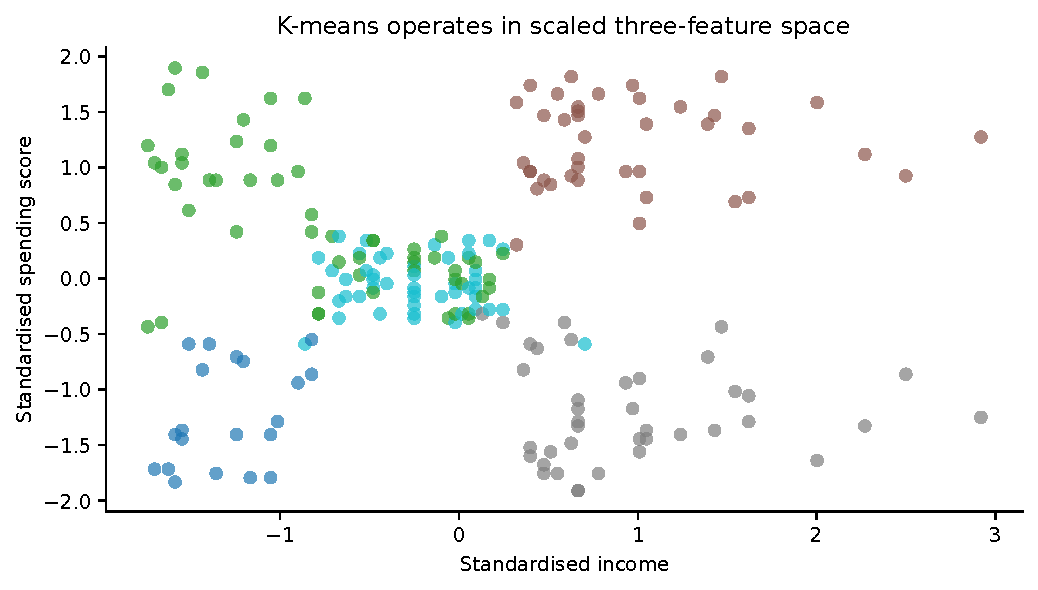
\includegraphics[width=0.76\linewidth]{figures/unsupervised_kmeans_clusters.pdf}
\end{utpfig}

\section{Distance defines what ``similar'' means}
K-means uses squared Euclidean distance, so its notion of similarity is geometric and roughly spherical around cluster centres. If meaningful groups differ by density, curved shape, categorical structure, or another distance notion, k-means may be a poor representation even when it returns a numerically stable solution.

Standardisation is therefore not a routine cosmetic step: it changes the geometry on which clusters are defined.


\section{Scale before distance-based clustering}
If one feature ranges from 0 to 1000 and another from 0 to 1, Euclidean distance is dominated by the larger scale. Standardisation makes distances reflect standard-deviation units rather than raw measurement magnitude.

\begin{pitfall}
Clusters are not automatically ``real'' categories. K-means will return \(k\) clusters even when the data have no natural grouping. Interpret clusters using stability, separation, domain meaning, and external information when available.
\end{pitfall}


\section{Initialisation and stability matter}
K-means can converge to different local solutions from different starting centres. Using multiple random initialisations and comparing the best within-cluster objective reduces this instability. More importantly, analysts should check whether broad cluster assignments persist across seeds or modest perturbations of the data.

\begin{utpfig}[Elbow curve for standardised Iris measurements]{Within-cluster sum of squares must decrease as more clusters are added. The useful question is whether there is a practically meaningful bend before improvements become small.}{fig:unsup-elbow}
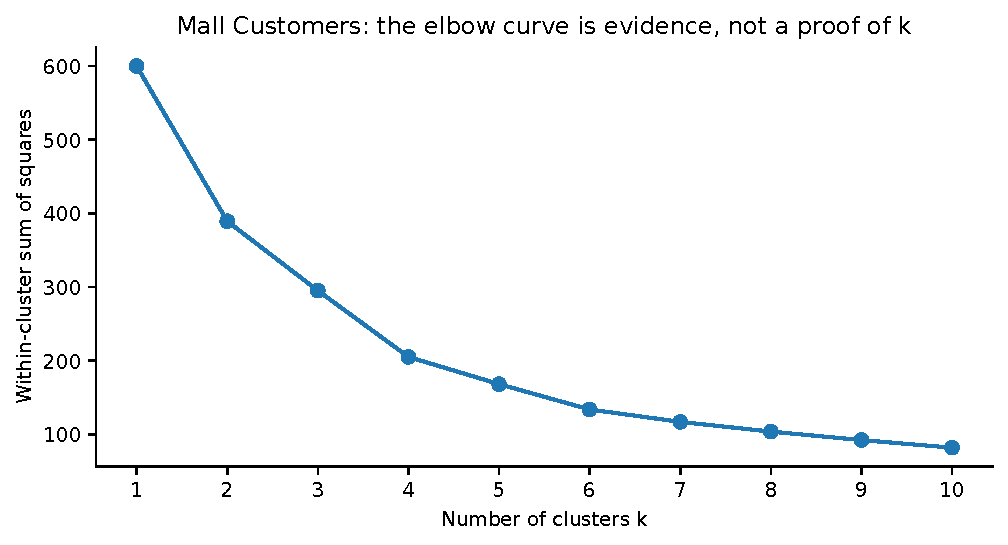
\includegraphics[width=0.78\linewidth]{figures/unsupervised_elbow.pdf}
\end{utpfig}

\section{Choosing \(k\) is a modelling decision}
Use several forms of evidence: within-cluster sum of squares, silhouette-style separation, stability across random starts or resamples, and domain usefulness. No elbow plot can replace interpretation.


\section{PCA is a rotation of the numeric feature space}
After centering the features---and often scaling them when units differ---PCA finds a first direction with maximum variance. The second direction is constrained to be perpendicular to the first and captures the greatest remaining variance, and so on. Because the directions are linear combinations of the original features, PCA is most useful when correlation creates redundancy.

\begin{utpfig}[Iris observations in the first two principal components]{The first two components retain most of the variance and reveal strong separation for setosa plus overlap between the other species. Species labels are shown only for interpretation.}{fig:unsup-pca-scores}
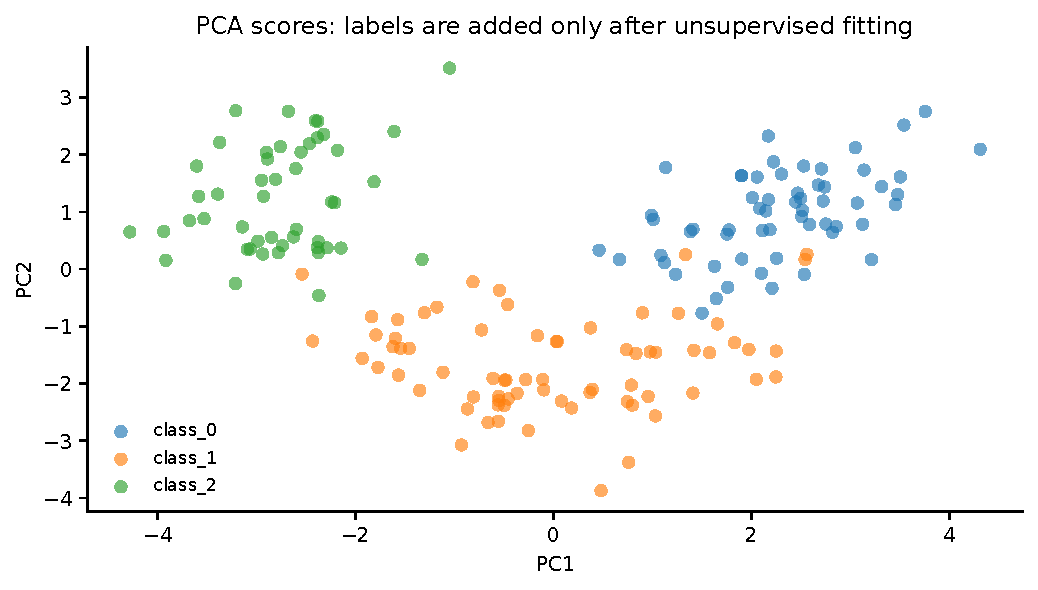
\includegraphics[width=0.76\linewidth]{figures/unsupervised_pca_scores.pdf}
\end{utpfig}

\begin{utpfig}[Explained variance by component]{The bars show variance captured by each component, while the cumulative line shows how quickly information is retained as more components are kept.}{fig:unsup-pca-variance}
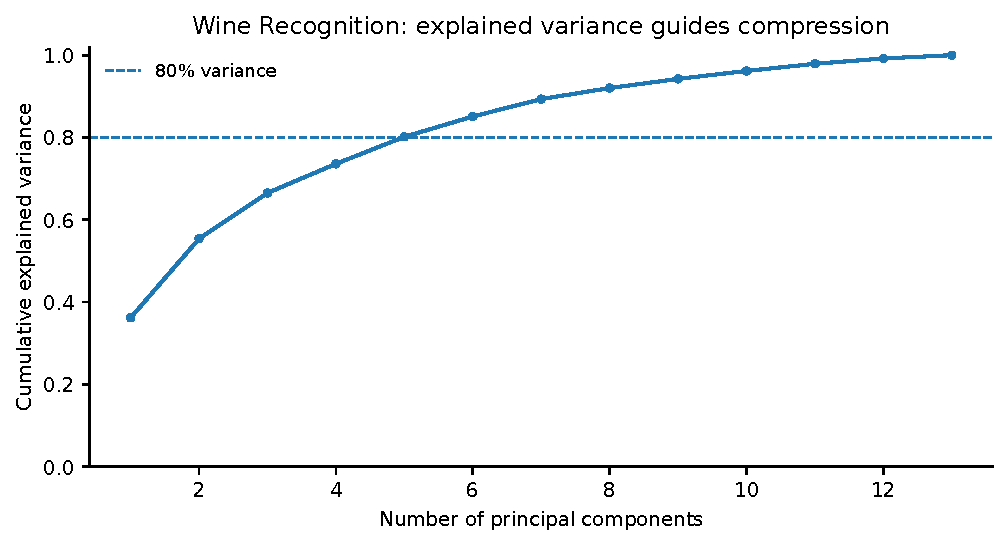
\includegraphics[width=0.78\linewidth]{figures/unsupervised_explained_variance.pdf}
\end{utpfig}

\section{Principal component analysis compresses correlated features}
\term{PCA} creates orthogonal linear combinations of the original numeric variables. The first component captures the greatest possible variance; later components capture remaining orthogonal variance.

\begin{utptable}
\begin{tabularx}{\linewidth}{@{}>{\bfseries\leavevmode\color{UTPNavy}}m{3.2cm}YD{4.1cm}@{}}
\toprule
\rowcolor{UTPPaleBlue!92}
\utpth{PCA object} & \utpth{Meaning} & \utpth{Use} \\
\midrule
Scores & coordinates of observations on components & plotting or modelling \\
Loadings & contribution of original features to components & interpretation \\
Explained variance & fraction of variability per component & decide dimensionality \\
\bottomrule
\end{tabularx}
\end{utptable}


\section{Loadings connect components back to original variables}
A principal-component score is difficult to interpret until the corresponding \term{loadings} are inspected. Large absolute loadings indicate variables that contribute strongly to that direction; signs indicate which variables move together or oppose one another along the component.

\begin{utpfig}[PCA loading directions]{Arrows show how the four standardised Iris measurements contribute to the first two principal components. Variables pointing in similar directions are positively related in this reduced space.}{fig:unsup-pca-loadings}
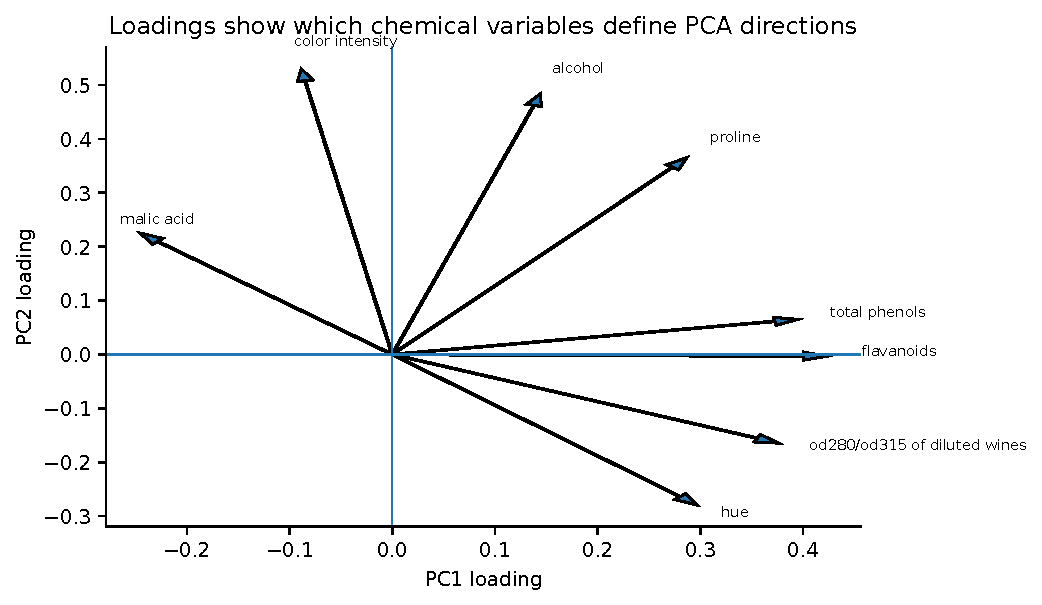
\includegraphics[width=0.70\linewidth]{figures/unsupervised_pca_loadings.pdf}
\end{utpfig}

\begin{pitfall}
PCA maximises variance, not predictive usefulness or interpretability. A low-variance direction can still be important for a specific target, and a high-variance component can reflect nuisance variation. Dimensionality reduction must be evaluated against the downstream purpose.
\end{pitfall}


\section{Labels can be used after clustering for interpretation}
In the Iris lab, species labels are excluded from k-means fitting. After the clusters are created, comparing cluster assignment with species can help interpret discovered structure. This is evaluation after fitting, not supervision during fitting.

\begin{keyidea}
Unsupervised methods discover mathematical structure. Human judgment is still required to decide whether that structure is stable, meaningful, actionable, or merely an artefact of scaling and algorithm choices.
\end{keyidea}

\begin{quickcheck}
\begin{enumerate}
  \item What information is missing in unsupervised learning compared with supervised learning?
  \item Why should numeric features often be standardised before k-means?
  \item Why does requesting three clusters not prove that three natural groups exist?
  \item What is the difference between PCA scores and loadings?
\end{enumerate}
\end{quickcheck}

\section{Beyond Iris: customer segmentation and chemical profiles}

Different unsupervised methods answer different structural questions. Mall Customers asks whether observations form useful geometric segments; Wine Recognition asks whether many correlated chemical measurements can be represented in fewer dimensions.

\begin{utpfig}[Mall-customer k-means segmentation]{K-means partitions customers in income--spending space around learned centres. The five colours are algorithmic clusters, not pre-existing customer categories.}{fig:unsup-mall}
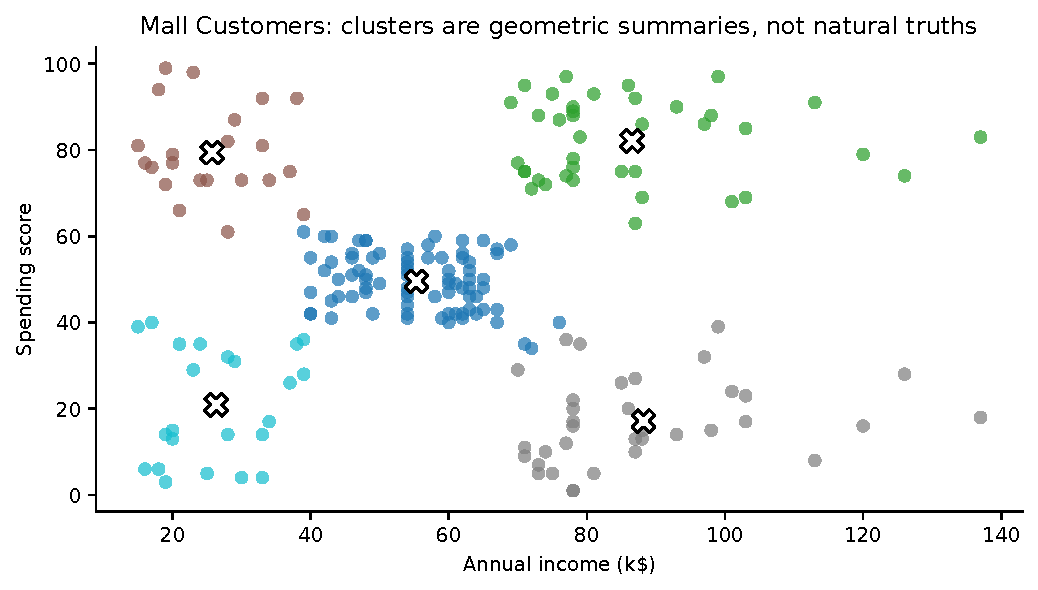
\includegraphics[width=0.78\linewidth]{figures/unsupervised_mall_clusters.pdf}
\end{utpfig}

The Mall Customers file has only 200 rows, but it is pedagogically useful because cluster meaning can be inspected in original units. Adding age changes the geometry even when the displayed plot uses only income and spending score; this reminds students that a two-dimensional visualisation can omit variables used by the algorithm.

\begin{utpfig}[Wine PCA compresses 13 standardised chemical measurements]{The cultivar labels are shown only after PCA has been fitted. Separation in score space helps interpret whether the unsupervised representation captures known chemical structure.}{fig:unsup-wine}
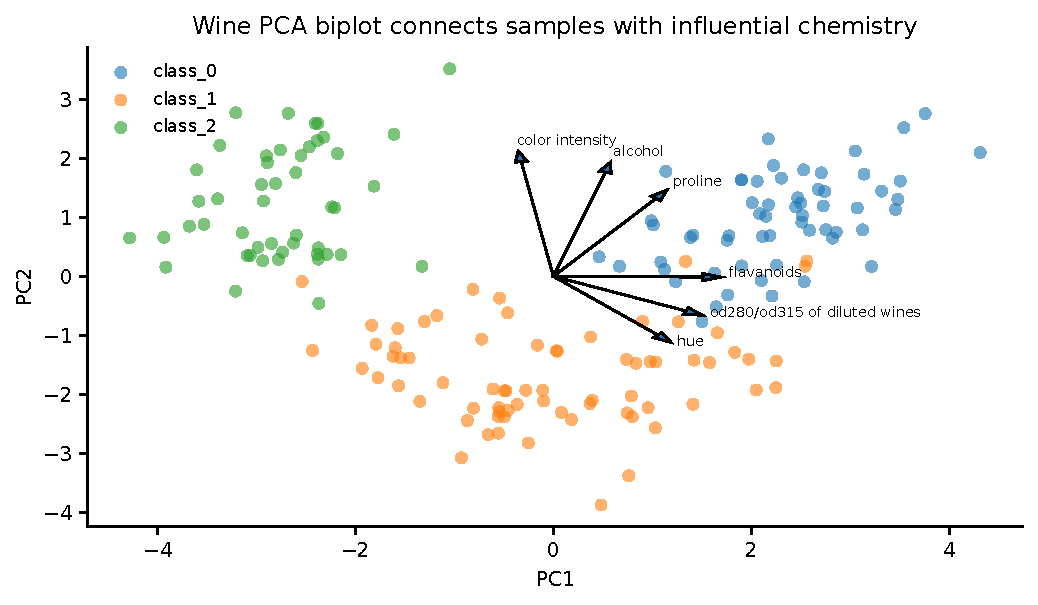
\includegraphics[width=0.80\linewidth]{figures/unsupervised_wine_pca.pdf}
\end{utpfig}

PCA is particularly appropriate here because the numeric variables are measured on different scales and many describe related chemical properties. Standardisation prevents variables with large raw units, such as proline or magnesium, from dominating simply because of their measurement scale.

\labsection{10}{Discover structure with clustering and PCA}{sec:lab10}

\begin{labproject}{Unsupervised learning: discover structure without inventing meaning}
\textbf{Coverage.} Chapter~\ref{ch:unsupervised}.\\
\textbf{Goal.} You should be able to standardise features for distance-based methods, assess cluster stability and choice of $k$, profile clusters in original units, fit PCA without label leakage, and interpret explained variance and loadings.\\
\textbf{Datasets.} \texttt{mall\_customers\_dataset.csv} and \texttt{wine\_recognition\_dataset.csv}.\\
\textbf{Scenario.} You have two unsupervised tasks: identify potentially useful customer groupings and compress correlated chemical measurements. In both cases, the algorithm returns mathematical structure; interpretation must be earned through diagnostics and domain context.

\textbf{Part A---k-means clustering.}
\begin{enumerate}
  \item Select age, annual income, and spending score; exclude identifiers. Standardise the features and explain why scale matters for Euclidean distance.
  \item Fit k-means for several candidate values of $k$ using multiple random starts. Record total within-cluster sum of squares and inspect whether an elbow is visible.
  \item Choose one $k$ as a working solution and rerun it with a large \texttt{nstart}. Report cluster sizes and centroids in the \emph{original units}.
  \item Plot income against spending score by cluster and explain what information is omitted because age is the third clustering dimension.
  \item Test stability by repeating the fit with different random seeds. Distinguish stable broad structure from assignments that change easily.
\end{enumerate}

\textbf{Part B---principal component analysis.}
\begin{enumerate}
  \item Exclude \texttt{sample\_id} and \texttt{cultivar} before PCA. Standardise all 13 chemical measurements.
  \item Report explained variance for the leading components and determine how many components are needed to capture a substantial proportion of total variance.
  \item Inspect the largest absolute loadings on PC1 and PC2 and describe which original chemical measurements drive those directions.
  \item Plot PC1 against PC2 without using cultivar labels during fitting. Introduce cultivar only afterward to assess whether known classes align with the unsupervised representation.
\end{enumerate}

\tcbbreak
\lstinputlisting[style=utpr]{all_experiments/lab10_unsupervised.R}
\begin{verification}
\textbf{Required evidence.} Submit one cluster-selection diagnostic, one cluster profile, one PCA explained-variance summary, and one score plot. For each task, write a two-sentence interpretation that separates the algorithmic result from the substantive meaning you are assigning to it.

\textbf{Professional standard.} Do not name clusters as customer ``types'' unless the labels are supported by stable feature profiles and a real decision context. Do not describe a principal component as a latent concept unless its loading pattern and domain meaning justify that interpretation.
\end{verification}
\end{labproject}



\part{Capstone}
\chapter{Capstone: An End-to-End Data-Science Analysis}
\label{ch:capstone}
\chapterguide
  {You should have completed the ten labs and be able to audit, explore, model, validate, and communicate tabular data.}
  {produce a compact, reproducible analysis in which every technical choice is connected to a question and every conclusion is connected to evidence.}

\section{The capstone is a workflow, not a bigger coding exercise}
Choose one bundled dataset or an instructor-approved external dataset. The goal is to demonstrate analytical judgment across the full lifecycle.

\begin{utpfig}[Capstone evidence chain]{A professional analysis keeps a visible line from the original question to the final limitations.}{fig:capstone-chain}
\begin{tikzpicture}[x=\linewidth,y=1cm,
  stage/.style={draw=UTPBlue!70,fill=UTPPaleBlue,rounded corners=1.5mm,
    line width=0.6pt,text width=0.155\linewidth,minimum height=1.55cm,
    inner xsep=1.8mm,inner ysep=2mm,align=center,
    font=\scriptsize\color{UTPNavy}},
  flow/.style={-{Stealth[length=2mm,width=1.5mm]},
    line width=0.8pt,draw=UTPTeal}]
\node[stage] (q) at (0,0) {\textbf{Question}\\[4pt]
  Define the goal\\and population};
\node[stage] (d) at (0.205,0) {\textbf{Data audit}\\[4pt]
  Check quality\\and provenance};
\node[stage] (e) at (0.410,0) {\textbf{EDA}\\[4pt]
  Explore patterns\\and relationships};
\node[stage] (m) at (0.615,0) {\textbf{Method}\\[4pt]
  Model or infer\\with justification};
\node[stage,draw=UTPTeal!80,fill=UTPPaleTeal] (v) at (0.820,0)
  {\textbf{Validation}\\[4pt]
   Assess evidence\\and state limits};
\draw[flow] (q.east) -- (d.west);
\draw[flow] (d.east) -- (e.west);
\draw[flow] (e.east) -- (m.west);
\draw[flow] (m.east) -- (v.west);
\end{tikzpicture}
\end{utpfig}


\section{Build the report around an evidence chain}
A capstone becomes easier to follow when every section answers one question. The introduction defines the target population and analytical goal. The data section establishes whether the observations are fit for purpose. EDA develops evidence and candidate explanations. The method section describes how uncertainty or generalisation is quantified. The conclusion states only what the design and validation support.

\begin{utpfig}[Recommended capstone report architecture]{The figure or table in each stage should answer a specific analytical question rather than exist merely to demonstrate a technique.}{fig:capstone-report-architecture}
\begin{tikzpicture}[node distance=0.24cm,
  stage/.style={draw=UTPBlue!70,fill=UTPPaleBlue,rounded corners=1.5mm,
    line width=0.6pt,text width=0.68\linewidth,minimum height=0.90cm,
    inner xsep=3mm,inner ysep=1.5mm,align=center,
    font=\scriptsize\color{UTPNavy}},
  endpoint/.style={stage,draw=UTPTeal!80,fill=UTPPaleTeal},
  flow/.style={-{Stealth[length=1.6mm,width=1.3mm]},
    line width=0.8pt,draw=UTPTeal}]
\node[endpoint] (q) {\textbf{1. Question and scope}\\[2pt]
  Target population and unit of observation};
\node[stage,below=of q] (audit) {\textbf{2. Data audit}\\[2pt]
  Data dictionary, quality checks, and exclusions};
\node[stage,below=of audit] (eda) {\textbf{3. Exploratory analysis}\\[2pt]
  3--5 purposeful figures with evidence sentences};
\node[stage,below=of eda] (method) {\textbf{4. Method and justification}\\[2pt]
  Inference, prediction, or structure discovery};
\node[stage,below=of method] (val) {\textbf{5. Validation}\\[2pt]
  Error analysis and sensitivity checks};
\node[endpoint,below=of val] (claim) {\textbf{6. Finding and implications}\\[2pt]
  Practical meaning, limitations, and next evidence};
\draw[flow] (q.south) -- (audit.north);
\draw[flow] (audit.south) -- (eda.north);
\draw[flow] (eda.south) -- (method.north);
\draw[flow] (method.south) -- (val.north);
\draw[flow] (val.south) -- (claim.north);
\end{tikzpicture}
\end{utpfig}

\section{Required components}
\begin{utpsteps}
  \item \textbf{Problem framing.} State the analytical question, target population, unit of observation, and why the answer would matter.
  \item \textbf{Data understanding.} Provide a data dictionary for variables used, source/provenance, shape, missingness, and quality constraints.
  \item \textbf{Preparation.} Show filters, cleaning rules, transformations, and feature engineering with counts of affected records.
  \item \textbf{EDA.} Include at least three purposeful visualisations and concise evidence sentences.
  \item \textbf{Method.} Use an appropriate inferential, supervised, or unsupervised method and justify why it matches the question.
  \item \textbf{Validation.} Use held-out data, cross-validation, uncertainty intervals, or stability checks appropriate to the method.
  \item \textbf{Communication.} State the main result, practical meaning, limitations, and a next step without overclaiming causality.
\end{utpsteps}


\section{Minimum visual standard}
Use at least three analytical figures, not including decorative diagrams. A strong submission normally includes one distribution or group-comparison view, one relationship or multivariate view, and one method-specific diagnostic such as a residual plot, confusion matrix, validation-fold chart, cluster view, or PCA projection.

Every figure should have a title or caption that answers: \emph{what should the reader notice, and why does it matter for the question?} Figures with no analytical interpretation do not strengthen the report.


\section{Suggested capstone directions}
\begin{utptable}
\begin{tabularx}{\linewidth}{@{}>{\bfseries\leavevmode\color{UTPNavy}}m{3.2cm}YD{5.0cm}@{}}
\toprule
\rowcolor{UTPPaleBlue!92}
\utpth{Dataset} & \utpth{Possible question} & \utpth{Suitable methods} \\
\midrule
Iris & Which measurements separate species and how does unsupervised structure compare? & EDA, PCA, k-means, classification extension \\
Wine recognition & Which chemical measurements are most associated with cultivar or alcohol? & EDA, inference, regression, multiclass extension \\
Breast cancer diagnostic & How do selected measurements separate diagnostic labels? & EDA, logistic classification, cross-validation \\
\bottomrule
\end{tabularx}
\end{utptable}

\begin{pitfall}
Do not choose a model first and then invent a question that fits it. The capstone is assessed on coherence of the evidence chain, not algorithm complexity.
\end{pitfall}


\section{Recommended checks before submission}
\begin{utpsteps}
  \item Restart R and run the analysis script from top to bottom using relative paths.
  \item Confirm that raw data files are not modified by the script.
  \item Compare row counts before and after every major filter or join.
  \item Verify that test or validation data do not influence learned preprocessing.
  \item Check that every reported number and figure can be reproduced from code.
  \item Read every claim and ask whether it is descriptive, predictive, or causal; revise wording that exceeds the design.
  \item State at least two limitations that could materially change the conclusion.
\end{utpsteps}


\section{Submission structure}
Submit one analysis script, one concise report, and any generated figures or derived data required to reproduce the result. The script should run from a clean session with local relative paths. The report should be readable without executing code.

\begin{keyidea}
A strong capstone makes uncertainty and limitations easy to find. Professional data science is credible because it exposes what could be wrong as clearly as what appears to be true.
\end{keyidea}


\end{document}
